%% LaTeX2e class for student theses
%% sections/apendix.tex
%% 
%% Karlsruhe Institute of Technology
%% Institute for Program Structures and Data Organization
%% Chair for Software Design and Quality (SDQ)
%%
%% Dr.-Ing. Erik Burger
%% burger@kit.edu
%%
%% Version 1.3.6, 2022-09-28

\iflanguage{english}
{\chapter{Appendix}}    % english style
{\chapter{Anhang}}      % german style
\label{chap:appendix}


%% -------------------
%% | Example content |
%% -------------------
\section{Proof of Data points trained using Active Learning}
\label{sec:appendix:FirstSection}
\begin{theorem}
Let $X$ be a set of data points of size $n$, $b < n, n \mod b = 0$ be the batch size. Then a machine learning model trained
using pool-based Active Learning is trained $\frac{n}{b}$ times on the current labeled pool of data points. Overall, the model
is trained on $\frac{n(n+b)}{2b}$ data points
\end{theorem}
\begin{proof}
    The first part is trivial, given that the model is trained until the labeled pool is exhausted and in each iteration $b$
    points are queried for their label. To determine the total number of points used, we need to sum up the number of points
    used in each iteration. 
    \begin{equation}
        \sum_{i=1}^{\frac{n}{b}} i \cdot b
    \end{equation}
    Using the formula for the sum of the first $n$ natural numbers, we get
    \begin{equation}
        \sum_{i=1}^{\frac{n}{b}} i \cdot b = b \cdot \sum_{i=1}^{\frac{n}{b}} i = b \cdot \frac{\frac{n}{b} (\frac{n}{b} + 1)}{2}
        = \frac{n (\frac{n}{b} + 1)}{2} = \frac{n(n+b)}{2b}
    \end{equation}
\end{proof}

\section{Experiment Setup}
\label{sec:Appendix:Setup}
In this section, we will list tables and figures containing the specifications of the hardware and software used in our experiments.

\subsection{Hardware}
\label{sec:Appendix:Hardware}
Since we run our experiments on BwUnicluster2.0, we provide a detailed list of the hardware specifications of the nodes we used. Please
note that this table only contains the nodes we used in our experiments. For a more detailed list of all nodes as well as all further
information, see \cite{bwUniclusterHardware}

\newpage

\begin{table}[!htb]
    \begin{tabularx}{\textwidth}{|X || X | X | X|} 
        \hline
         & GPU x4 & GPU x8 & GPU x4 A100 \\ 
        \hline
        \hline 
        Processors & Intel Xeon Gold 6230 & Intel Xeon Gold 6248 & Intel Xeon Platinum 8358  \\ 
        \hline
        Number of sockets & 2 & 2 & 2  \\ 
        \hline
        Processor frequency (GHz) & 2.1 & 2.6 & 2.5  \\ 
        \hline
        Total number of cores & 40 & 40 & 64  \\ 
        \hline
        Main memory & 384 GB & 768 GB & 512 GB  \\ 
        \hline
        Local SSD & 3.2 TB NVMe & 15TB NVMe & 6.4 TB NVMe  \\ 
        \hline
        GPUs & 4x NVIDIA Tesla V100 & 8x NVIDIA Tesla V100 & 4x NVIDIA A100  \\ 
        \hline
        GPU Memory & 32 GB  & 32 GB & 80 GB  \\ 
        \hline
        Interconnect & IB HDR & IB HDR & IB HDR200  \\ 
        \hline
    \end{tabularx}
    \caption{Hardware configuration for the three nodes used on BWUniCluster2.0. }
    \label{fig:HardwareSpec}
\end{table}


\subsection{Software}
\label{sec:Appendix:Software}
In this section, we provide a comprehensive list of the libraries we used in our experiments as well as their version
and a link to their documentation.

\begin{table}[!htb]
    \centering
    \begin{tabular}{|l || l | l |} 
        \hline
        Library Name & Version & Link \\ 
        \hline 
        \hline
        numpy & 1.23.0 & \url{https://numpy.org/} \\
        \hline
        tqdm & 4.64.1 & \url{https://tqdm.github.io/}  \\
        \hline
        torchvision & 0.14.1 & \url{https://pytorch.org/vision/stable/index.html} \\ 
        \hline
        torch & 1.13.1 & \url{https://pytorch.org/} \\
        \hline
        PyYAML & 6.0 & \url{https://pyyaml.org/} \\
        \hline
        scipy & 1.10.1 & \url{https://scipy.org/} \\
        \hline
        scikit-learn & 1.2.1 & \url{https://scikit-learn.org/stable/index.html} \\
        \hline
        wget & 3.2 & \url{https://pypi.org/project/wget/} \\
        \hline
    \end{tabular}
    \caption{Software Libraries used for the experiments}
    \label{fig:Libraries}
\end{table}

\subsection{Continual Learning strategies}
\label{sec:Appendix:CLStrategies}
In this section, we extend the parameter description of the Continual Learning strategies given in section 
\ref{sec:ExperimentSetup:CLStrategies} by presenting a table for with the exact hyperparameter configuration
used in the experiments.

\begin{table}[!htb]
    \begin{tabularx}{\textwidth}{|l | X | l |} 
        \hline
        Hyperparameter & Description & Value \\ 
        \hline 
        \hline
        $\lambda$ & Balances between old and new tasks. A higher value indicates more focus 
        on preserving knowledge from the old task & 1.0  \\ 
        \hline
        Sample size & Relative size of the sample compared to the full training set that is used to 
        compute the Fisher Matrix & 0.05  \\ 
        \hline
        Gradient Clip & Maximum Value of the $l2$-Norm of the gradient. If the current norm is larger,
        the gradient is clipped to that value & 20.0 \\ 
        \hline
    \end{tabularx}
    \caption{Hyperparameter configuration for \gls{ewc}.}
    \label{fig:EWCparams}
\end{table}

\begin{table}[!htb]
    \begin{tabularx}{\textwidth}{| l | X | l |} 
        \hline
        Hyperparameter & Description & Value \\ 
        \hline 
        \hline
        $\lambda$ & Balances between old and new tasks. A higher value indicates more focus
        on preserving knowledge \newline from the old task & 1.0  \\ 
        \hline
        Gradient Clip & Maximum Value of the $l2$-Norm of the gradient. If the current norm is larger, the
        gradient is clipped to that value & 2.0 \\ 
        \hline
    \end{tabularx}
    \caption{Hyperparameter configuration for \gls{mas}.}
    \label{fig:MASparams}
\end{table}

\begin{table}[!htb]
    \begin{tabularx}{\textwidth}{| l | X | l |} 
        \hline
        Hyperparameter & Description & Value \\ 
        \hline 
        \hline
        $\lambda$ & Balances between old and new tasks. A higher value indicates more focus
        on preserving knowledge from the old task & 1.0  \\ 
        \hline
        Gradient Clip & Maximum Value of the $l2$-Norm of the gradient. If the current norm is larger, the
        gradient is clipped to that value & 20.0 \\ 
        \hline
        $\alpha$ & Weights the importance of the previous tasks. The sum of all $\alpha$ values must be 1.0 & 0.45,0.55 \\
        \hline
    \end{tabularx}
    \caption{Hyperparameter configuration for \gls{imm}.}
    \label{fig:IMMparams}
\end{table}

\begin{table}[!htb]
    \centering
    \begin{tabularx}{\textwidth}{| l | X | l |} 
        \hline
        Hyperparameter & Description & Value \\ 
        \hline 
        \hline
        $a$ & Balances between old and new tasks. A higher value indicates more focus
        on preserving knowledge from the old task & 0.5  \\ 
        \hline
        $a'$ & Used to update parameter importances in Equation \hyperref[eq:ALASSO_Small_Omega]{3.23} & 0.25  \\
        \hline
        Gradient Clip & Maximum Value of the $l2$-Norm of the gradient. If the current norm is larger, the
        gradient is clipped to that value & 2.0 \\ 
        \hline
        $c$ & Determines the overestimation of the loss on the unobserved side & 3.0 \\
        \hline
        $c'$ & Used to update parameter importances in Equation \hyperref[eq:ALASSO_Small_Omega]{3.23} & 1.5 \\
        \hline
    \end{tabularx}
    \caption{Hyperparameter configuration for \gls{alasso}.}
    \label{fig:AlassoParams}
\end{table}

\subsection{Datasets}
\label{sec:Appendix:Datasets}

\begin{table}[!htb]
    \centering
    \begin{tabularx}{\textwidth}{|X || X | X | X | X|} 
        \hline
         & MNIST & CIFAR-10 & Tiny \newline ImageNet & Small \newline ImageNet \\ 
        \hline 
        \hline
        Size of training set & 60000 & 50000 & 100000 & 128116 \\ 
        \hline
        Size of validation set & 10000 & 10000 & 10000 & 50000\\
        \hline
        Number of classes & 10 & 10 & 200 & 1000 \\
        \hline
        Image Dimension & 28x28 & 32x32 & 64x64& 32x32\\
        \hline
        Number of channels & 1 & 3 & 3 & 3 \\
        \hline
        Source & torchvision & torchvision & {\small \url{http://cs231n.stanford.edu/tiny-imagenet-200.zip}} & {\small \url{http://www.image-net.org/data/downsample/Imagenet32_32.zip}} \\
        \hline
    \end{tabularx}
    \caption{Information on the datasets used for the experiments.}
    \label{fig:DatasetInformtion}
\end{table}

\subsection{Neural Network Architectures}
\label{sec:Appendix:Architectures}
In our experiments with Model Stealing, we use the same architectures as proposed in \cite{pal2020activethief}. Pal et al. propose a proprietary
\gls{cnn} architecture family which consists of $l$ convolution blocks followed by a single fully connected layer. Each convolution block consists
of 
\begin{enumerate}
    \item a convolutional layer with $k$ filters size $3 \times 3$,
    \item a ReLU activation layer,
    \item a batch normalization layer,
    \item a convolutional layer with $k$ filters size $3 \times 3$,
    \item a ReLU activation layer,
    \item a batch normalization layer,
    \item a max pooling layer with kernel size $2 \times 2$,
\end{enumerate}
where $k=32 \cdot 2^{i-1}$ is the number of filters for block number $i \in \{1,\ldots,l\}$.

\begin{figure}[!htb]
    \centering
    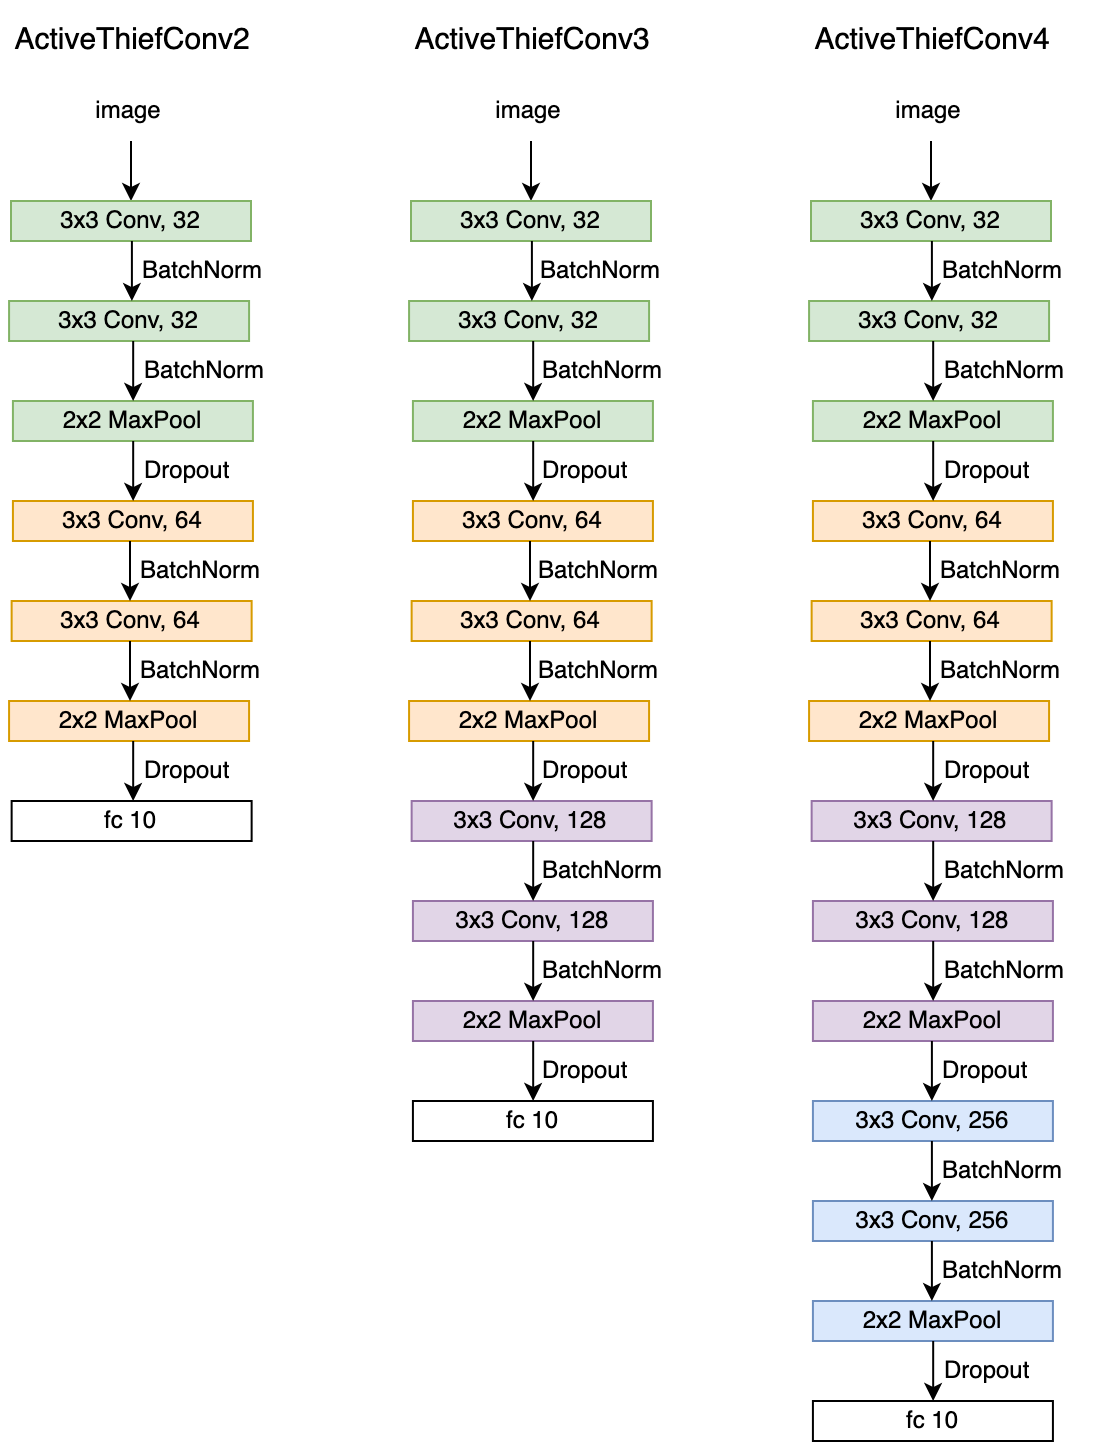
\includegraphics[width=\linewidth]{images/ActiveThiefConvs.png}
    \caption[ActiveThiefConv Architectures]{Example Network Architectures for CIFAR-10.}
    \label{fig:ActiveThiefArchitectures}
\end{figure}



\section{Continual Active Learning}
\label{sec:Appendix:ContinualActiveLearning}
In figure \ref{fig:Evaluation:Results:CAL:Random1000} we present the results of running the Active Learning strategy Random with the Continual Learning strategies Naive, \gls{ewc}, \gls{mas}, \gls{alasso} and \gls{imm}
as well as the baseline of running pure Active Learning. We use a batch size of 1000 for these experiments. In terms of runtime, all strategies are significantly faster than the classic Active
Learning approach. \gls{mas}, \gls{imm}, \gls{ewc} and Naive all are approximately 50 times as fast as the classic Active Learning approach. \gls{alasso} is slightly slower than the other Continual Learning strategies,
but still about 25 times faster than the baseline. However, there is a notable gap in validation accuracy between Active Learning and all Continual Active Learning strategies. \gls{imm} is the only
Continual Learning strategy to outperform the Naive approach. \gls{ewc} performs slightly worse Naive while \gls{mas} and \gls{alasso} perform significantly worse. While the validation accuracy of \gls{mas} increases only
slightly with an increasing size of the labeled pool, \gls{alasso} has an erratic validation curve which does not seem to stabilize until the end of the experiment. \par

Next, we run the same experiment setup with the Active Learning strategy \gls{lc}. Results can be found in figure \ref{fig:Evaluation:Results:CAL:LC1000}. Again, all Continual Learning strategies
are significantly outperform the baseline in terms of execution time. \gls{alasso} is the slowest Continual Learning strategy, albeit being roughly 25 times faster than the baseline. The remaining Continual
Learning strategies, \gls{imm}, \gls{mas}, CoreSet and \gls{ewc}, are all about 50 times faster than the baseline. The gap in validation accuracy between Active Learning and all Continual Active Learning strategies
remains similar to the gap observed with Random. \gls{imm} and Naive perform similarly, outperforming the remaining Continual Learning strategies in the first half of the experiment. \gls{ewc} picks up on their
performance in the after 25000 sampled data. \gls{mas} and \gls{alasso} fall behind in terms of performance, with \gls{alasso} experiencing significant accuracy drops. \gls{mas}' validation accuracy remain stable throughout
the whole experiment, catching up to the other Continual Learning strategies in the end. \par


\gls{bald} is the third Active Learning strategy we evaluate. Again, we use the same experiments setup as in the previous two experiments, changing only the Active Learning strategy but leaving every-
thing else as-is. The results of these experiments can be found in figure \ref{fig:Evaluation:Results:CAL:BALD1000}. In terms of runtime, the pattern established using \gls{lc} and Random continues.
\gls{mas}, \gls{imm}, \gls{ewc} and Naive are approximately 50 times as fast as the baseline, while \gls{alasso} is about 25 times as fast. Considering validation accuracy, all Continual Learning strategies perform significantly
worse than the baseline. Establishing a ranking between the Continual Learning strategies is difficult however, because they are all very erratic. \gls{alasso} stands out with the best and worst validation
accuracy, depending on the number of labeled samples. \gls{imm}, \gls{mas}, Naive and \gls{ewc} all have similar validaiton accuracy curves, although they are less erratic than \gls{alasso}. \par


After running our experiment with \gls{bald}, we re-run it using the Active Learning strategy CoreSet. We present the results in figure \ref{fig:Evaluation:Results:CAL:CoreSet1000}. The runtime of the 
Continual Learning strategies is again significantly lower than that of the baseline, however it is higher than in the previous experiments. \gls{alasso} is the slowest Continual Learning strategy, being
around 12 times as fast as the baseline. \gls{imm}, \gls{mas}, \gls{ewc} and Naive have a similar execution time and are approximately 15 times as fast as Active Learning using CoreSet. Just as in the previous experiments,
there is a significant gap in validation accuracy between the baseline and all Continual Learning strategies. \gls{imm}, \gls{ewc} and Naive perform almost similarly while \gls{mas} and \gls{alasso} fall behind. While \gls{mas} demon-
strates a marginally increasing validation accuracy, the validation accuracy curve of \gls{alasso} is unstable with significant drops and jumps in accuracy as the number of labeled data increases. \par


In our final experiment with batch size 1000, we use the Active Learning strategy \gls{badge}. The results are shown in figure \ref{fig:Evaluation:Results:CAL:Badge1000}. All Continual Learning strategies
outperform the baseline in terms of runtime by a large margin. Between the Continual Learning strategies, there are only marginal differences in execution time. The validation accuracy of all Continual
Learning strategies is irregular and all of them leave a significant gap to the baseline. There is no Continual Learning strategy which demonstrates a significantly higher or lower validation accuracy
than the others. However, \gls{mas} and \gls{alasso} fall behind the other Continual Learning strategies at around 25000 samples but manage to catch up in the end. \par


After running the experiment with \gls{badge}, CoreSet, \gls{lc}, \gls{bald} and Random, we perform the same experiment with Random but increase the batch size from 1000 to 2000. We present the results in
Figure \ref{fig:Evaluation:Results:CAL:Random2000}. The execution time remains significantly lower for all Continual Learning strategies compared to the baseline, however, the gap has decreased. 
\gls{alasso} is the slowest Continual Learning Strategy, being about 8 times as fast as the baseline. \gls{mas}, \gls{imm}, \gls{ewc} and Naive have similar execution times, being about 10 times as fast as the baseline. 
The gap in validation accuracy between the baseline and the Continual Learning strategies is still significant, however, it has decreased compared the experiment with a batch size of 1000.
\gls{ewc} outperforms all Continual Learning strategies, including Naive, although the gap between the two is marginal. \gls{alasso}, \gls{imm} and \gls{mas} perform show similar overall performance although the course
of their validation accuracy curves differ greatly. \gls{imm} starts worst and ends best. \gls{mas} shows similar performance to \gls{alasso} but is outperformed within the final 5000 samples. \par


Second, we run the experiment with batch size 2000 for the Active Learning strategy \gls{lc}. Our results can be found in figure \ref{fig:Evaluation:Results:CAL:LC2000}. Like in the previous experiment,
the gap in execution time between the baseline and the Continual Learning strategies has shrunk compared to the experiment with a batch size of 1000. Again, \gls{alasso} is the slowest Continual Learning
strategy, being approximately 9 times as fast as the baseline. \gls{ewc} is the second slowest strategy, being only marginally slower than \gls{mas}, \gls{imm} and Naive, who have a very similar execution time.
In terms of validation accuracy, there is still a significant gap between the baseline and the Continual Learning strategies. \gls{imm}, \gls{ewc} and Naive perform similar for the first 35000 samples, outperforming
\gls{mas} and \gls{alasso}. In the final 15000 samples, all \gls{imm}, \gls{ewc} and Naive experience a drop in validation accuracy, which is most significant for \gls{ewc}. The accuracy of \gls{mas} increases modestly until the labeled
pool contains 40000 samples, before dropping of by about 10\%. The validation accuracy curve of \gls{alasso} is again unstable, showing a slight downward trend over the course of the experiment. \par


We follow up with the experiment using the Active Learning strategy \gls{bald}, all other parameters being equal. The results can be found in figure \ref{fig:Evaluation:Results:CAL:BALD2000}. The gap in
execution time between the baseline and the Continual Learning strategies has declined compared to the experiment with \gls{bald} and batch size 1000. Naive and \gls{imm} are the fastest Continual Learning strategies,
closely followed \gls{ewc} and \gls{mas}. \gls{alasso} follows last, but is still about 10 times as fast as the baseline. The validation accuracy curves of most Continual Learning strategies are similar, with \gls{alasso} falling 
out of line. \gls{ewc}, \gls{imm} and Naive perform similar across the whole experiment with \gls{mas} starting off better but falling behind after approximately 15000 samples. \gls{alasso} performs on par with the remaining strategies
at first, but suffers from a heavy decrease in validation accuracy at around 15000 samples. All Continual Learning strategies leave a large gap to the baseline in terms of validation accuracy. \par

Next, we run the experiment with CoreSet and a batch size of 2000. We present our results in figure \ref{fig:Evaluation:Results:CAL:CoreSet2000}. The gap in execution time between the baseline and the
Continual Learning strategies has again decreased. \gls{imm} is the fastest Continual Learning strategy, closely followed by \gls{ewc}. \gls{ewc} is followed by Naive and \gls{mas}, who have similar execution times. \gls{alasso} is
the slowest approach, albeit being about 6.5 times as fast as the baseline. Regarding validation accuracy, all Continual Learning strategies are significantly outperformed by the baseline. Naive performs best
in the first half of the experiment, followed by \gls{ewc}, \gls{imm} and \gls{mas}. At around 25000 samples, the validation accuracy of \gls{imm}, \gls{ewc} and Naive suddenly becomes erratic, followed by a moderate increase in validation
accuracy and a drop in the final 10000 samples. \gls{mas} performs consistent but worse than \gls{imm}, \gls{ewc} and Naive, experiencing a moderate drop in validation accuracy in the final 10000 samples. \gls{alasso} performs worst,
with its validation accuracy decreasing over the course of the experiment. \par


Finally, we run the same experiment with the Active Learning strategy \gls{badge}. Our results can be found in figure \ref{fig:Evaluation:Results:CAL:Badge2000}. The margin in execution time between the baseline
and the Continual Learning strategies has decreased which is mainly due to the large decrease in runtime of the baseline, compared to the experiment with 1000 batch size. Nevertheless, the Continual
Learning strategies are about 3.5 times as fast as the baseline. Within the Continual Learning strategies there is only a minor runtime difference, with \gls{imm} being the fastest and \gls{alasso} the slowest. In terms of 
validation accuracy, the gap between the baseline as the Continual Learning strategies has decreased. More notably though, the validation accuracy curves of all Continual Learning strategies more consistent than
in the previous experiment with 1000 batch size. \gls{imm}, \gls{ewc} and Naive perform similar, followed by \gls{mas}. \gls{alasso} is the worst performing strategy, falling behind the others after bout 10000 samples. \par

\begin{figure}[h]
    \centering
    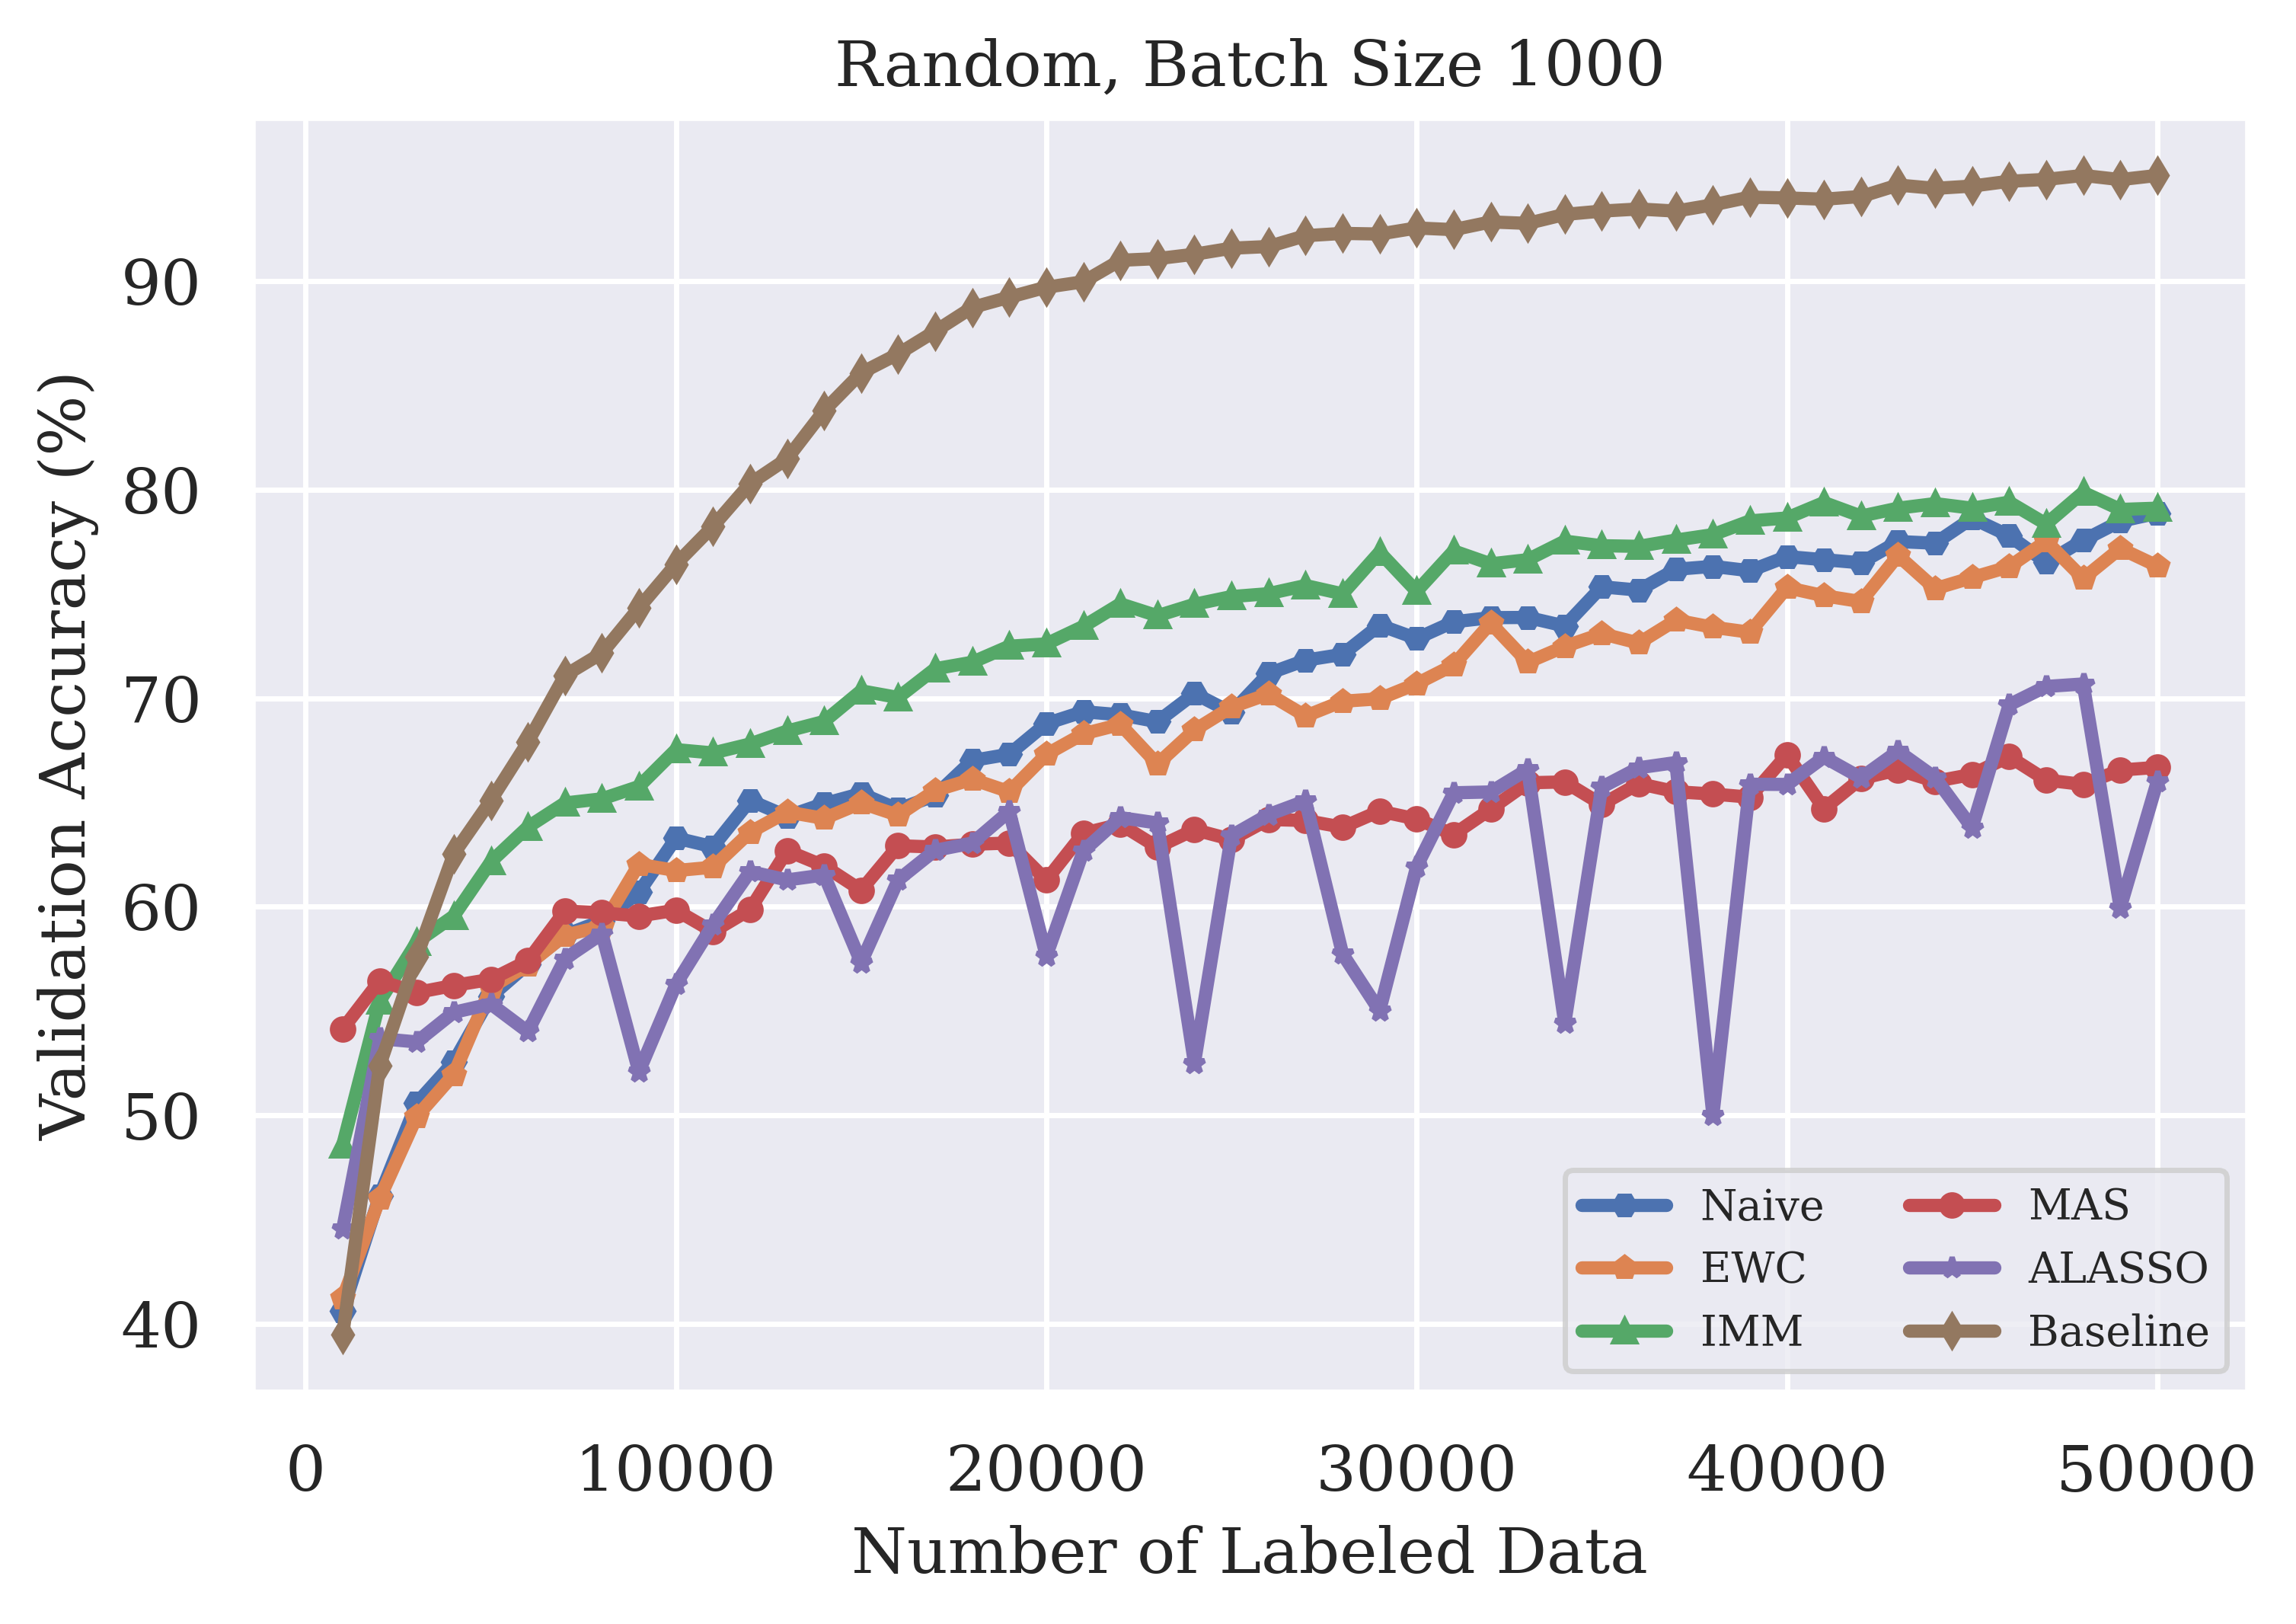
\includegraphics[width=0.32\linewidth]{images/results_CAL/random_1000b_acc.png} \hfill
    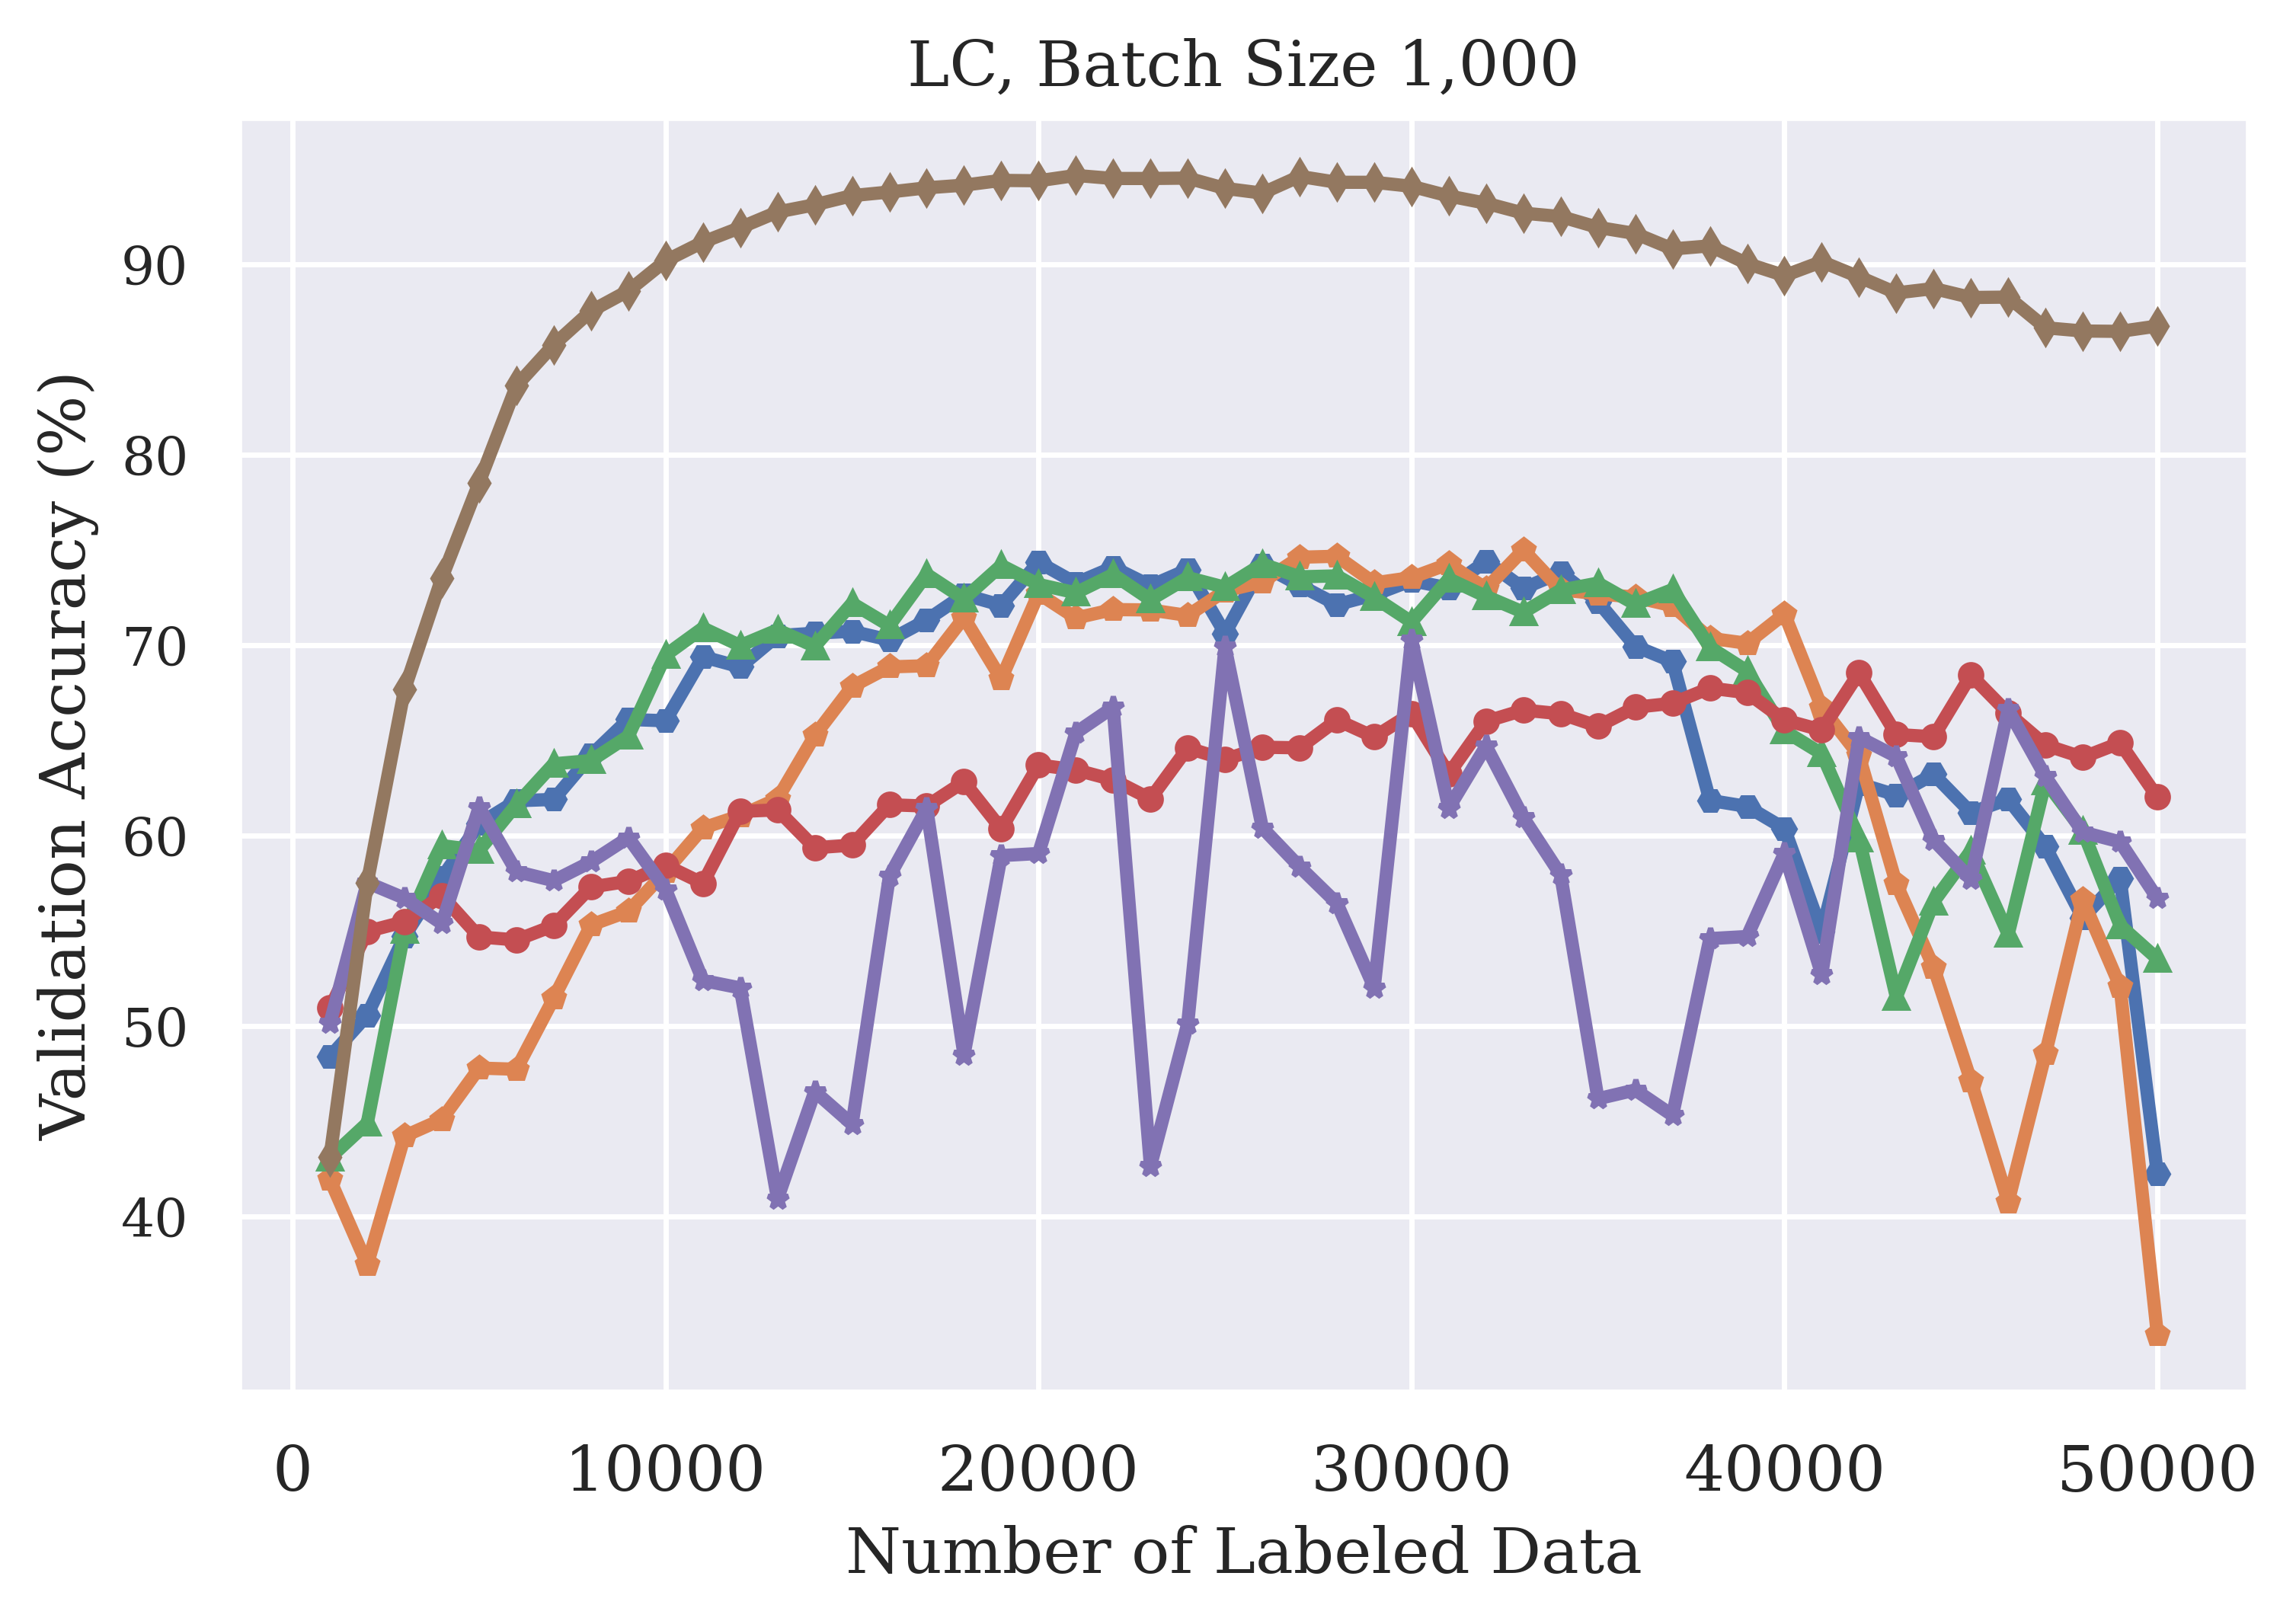
\includegraphics[width=0.32\linewidth]{images/results_CAL/lc_1000b_acc.png} \hfill
    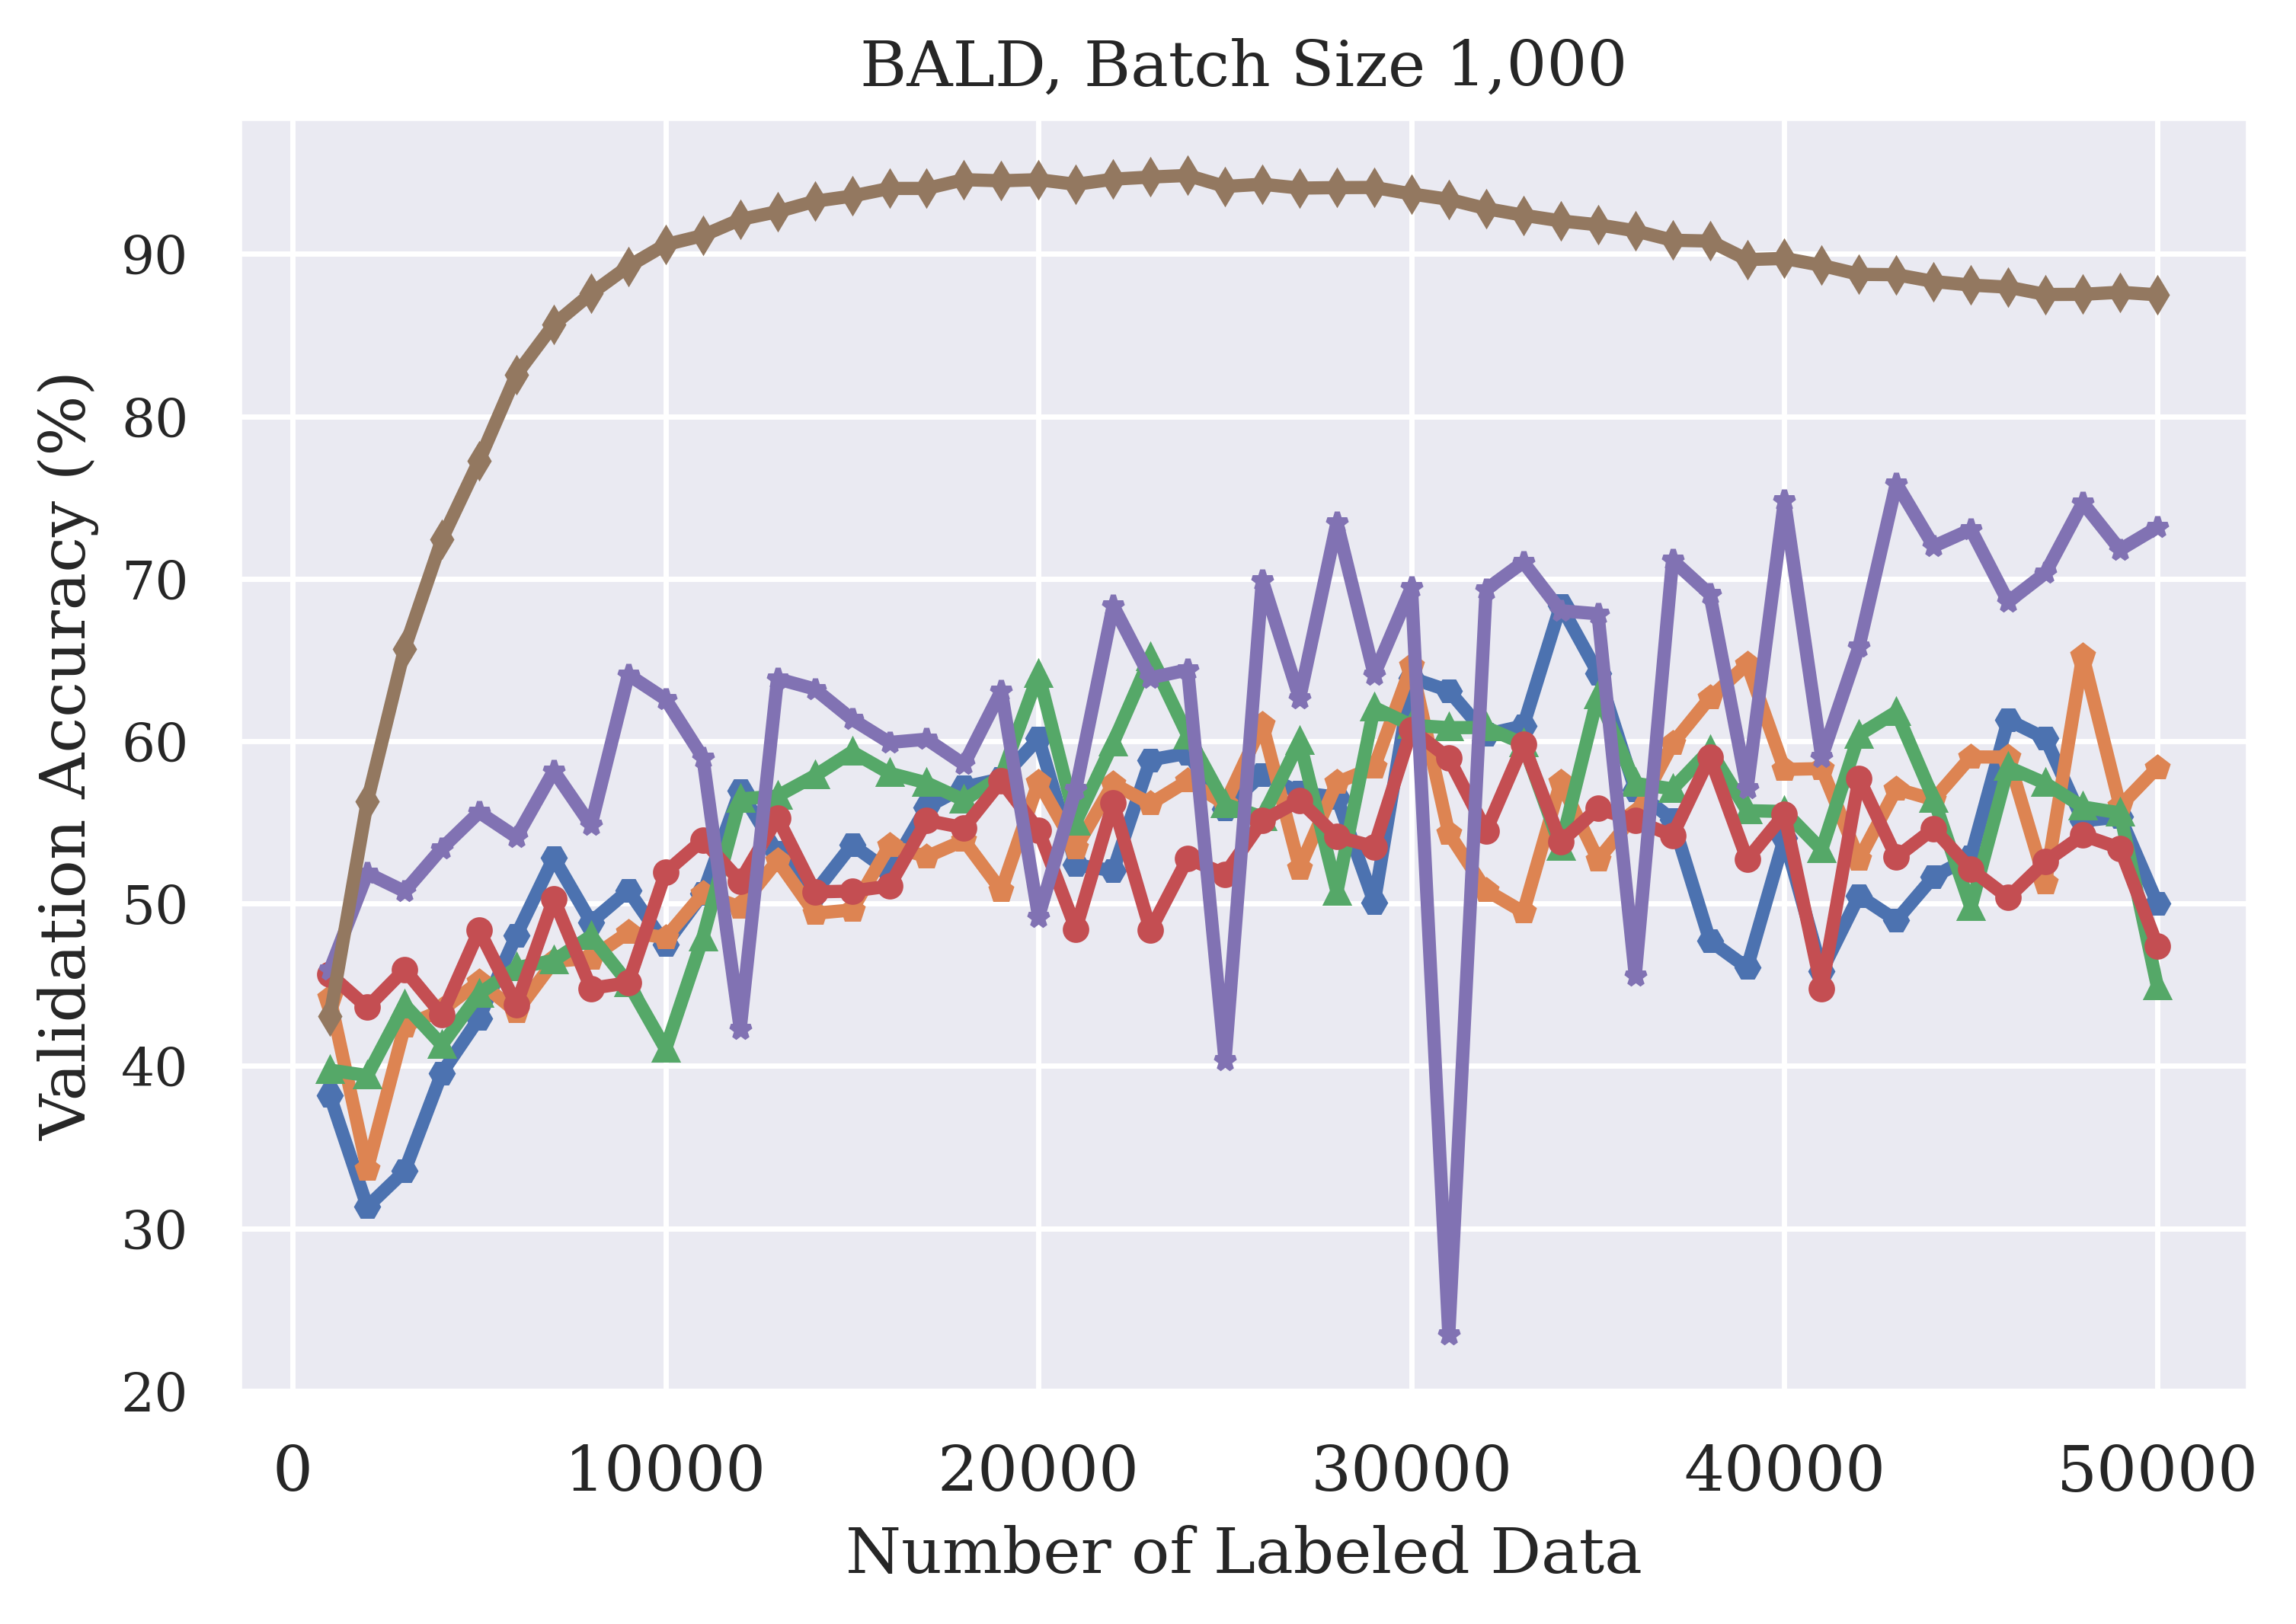
\includegraphics[width=0.32\linewidth]{images/results_CAL/bald_1000b_acc.png}
    \\[\smallskipamount]
    \hfill 
    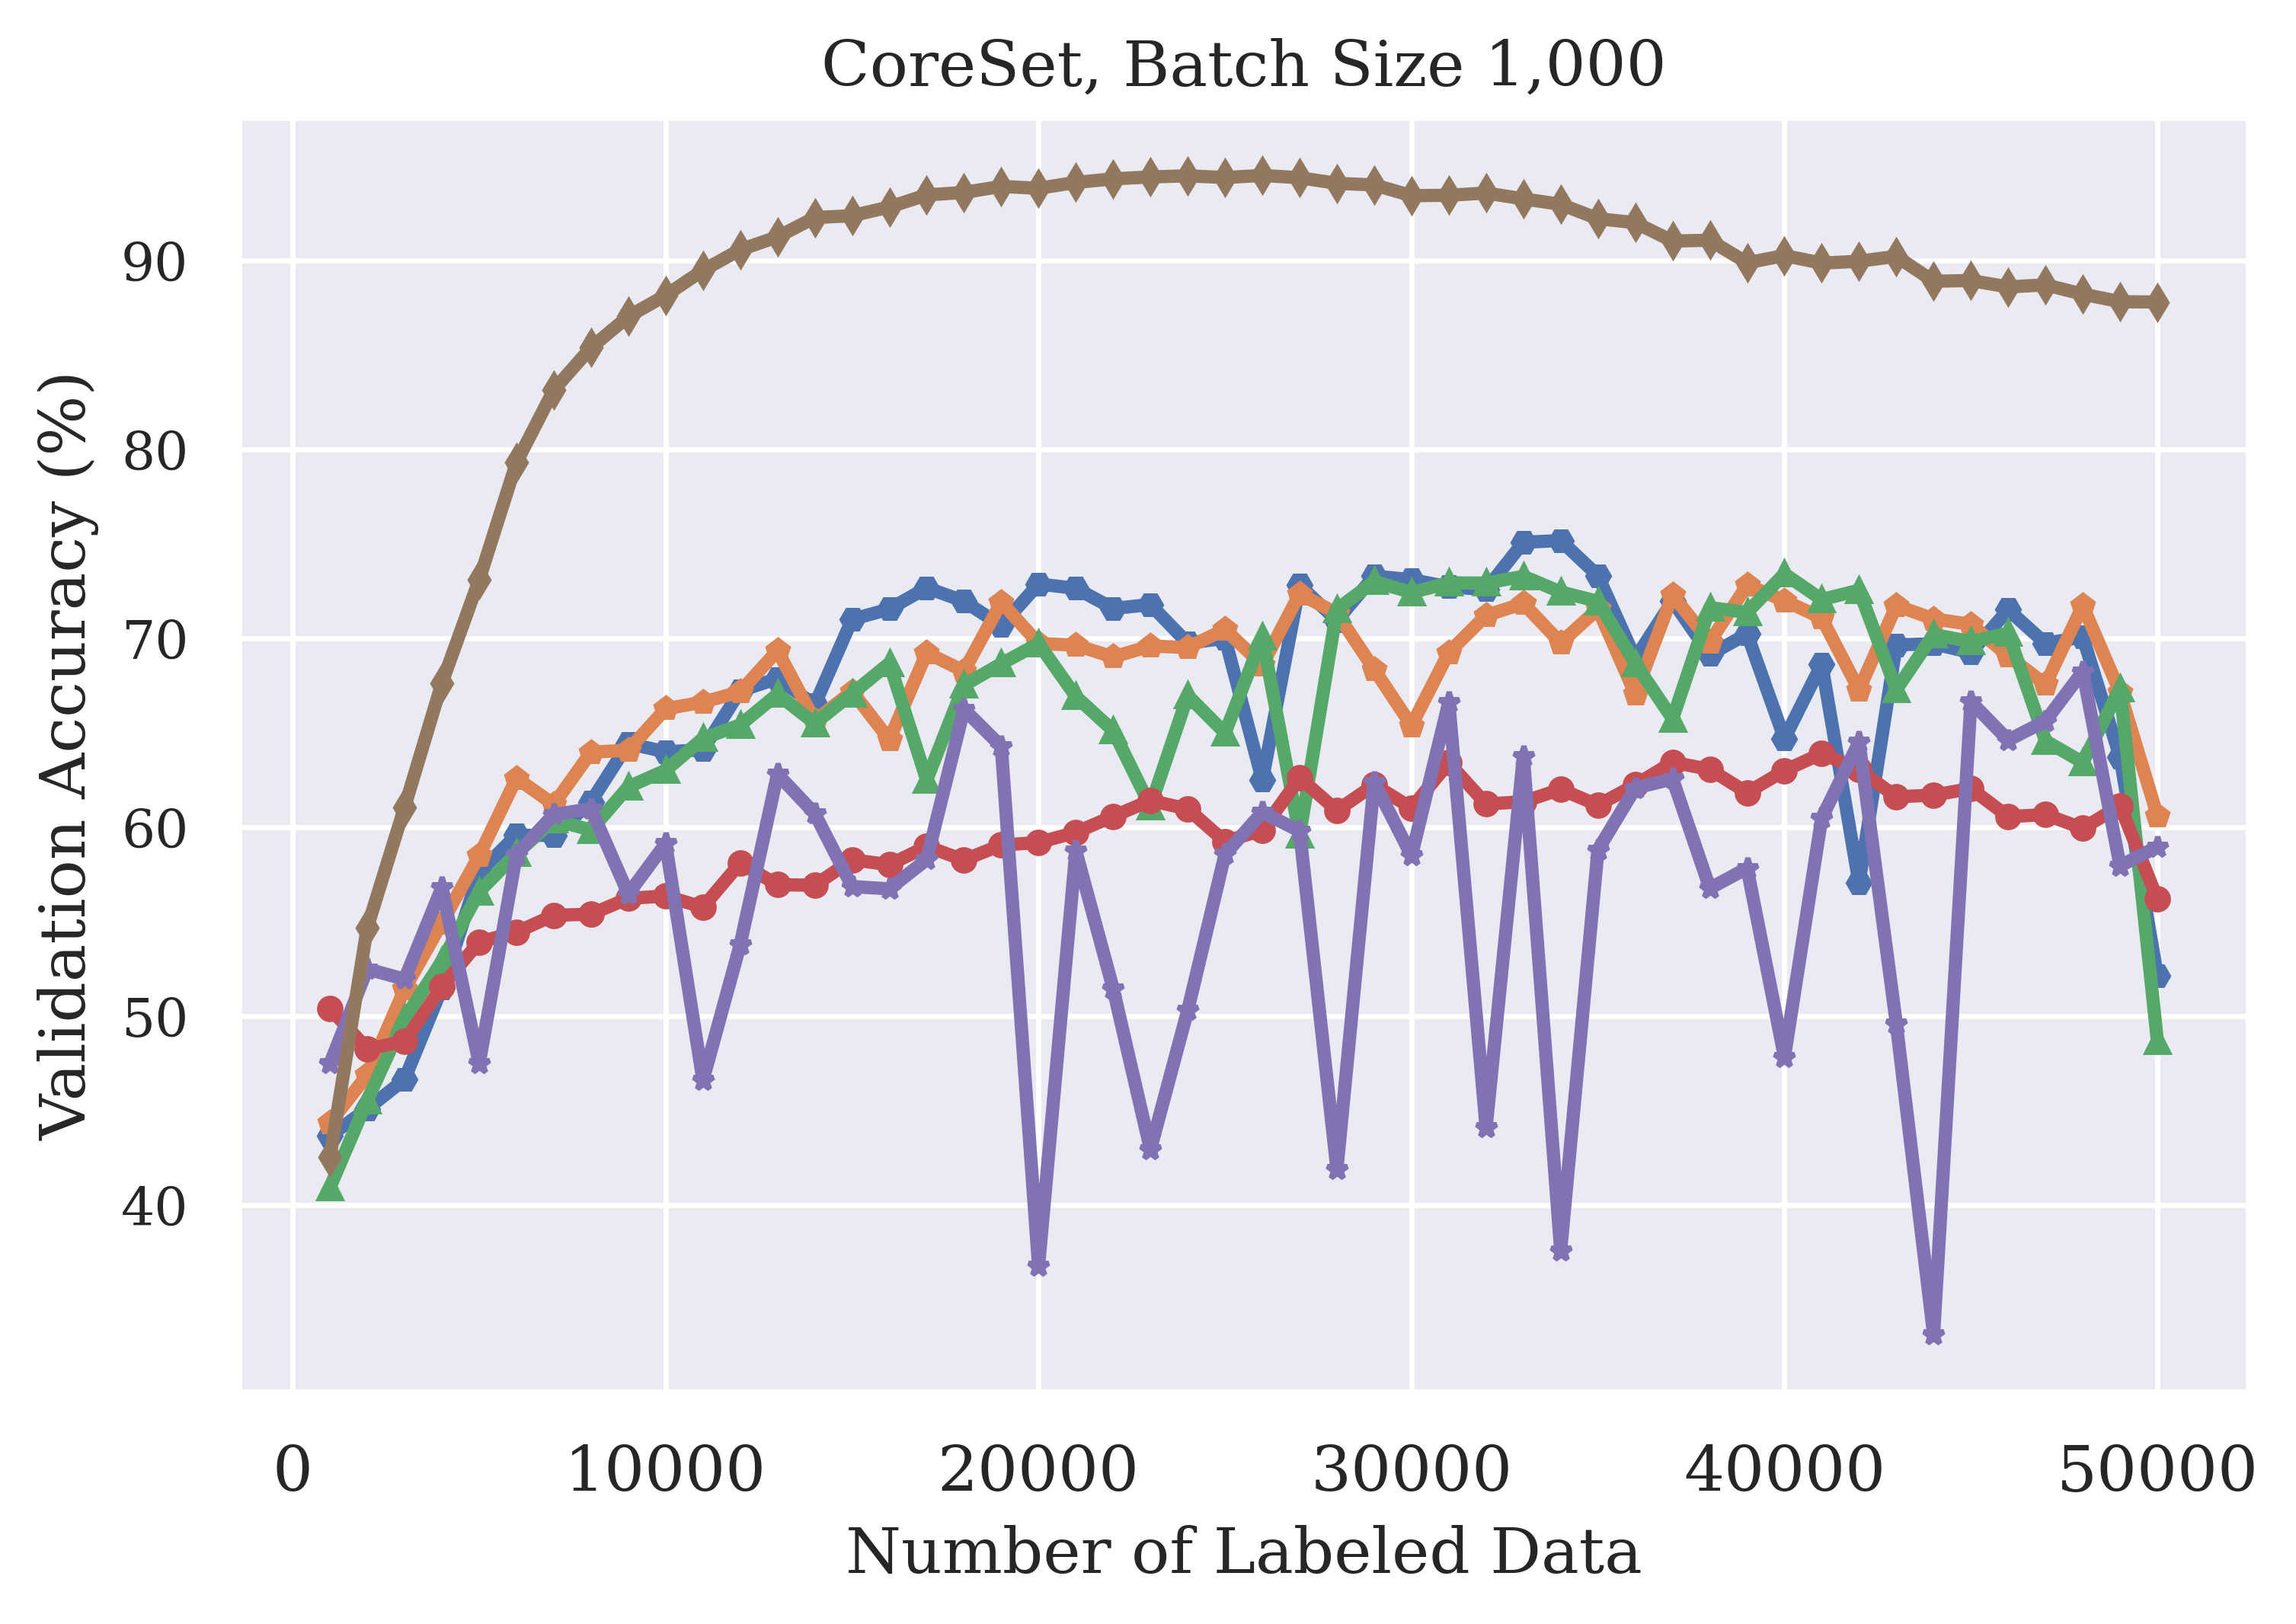
\includegraphics[width=0.32\linewidth]{images/results_CAL/coreset_1000b_acc.png} \hfill
    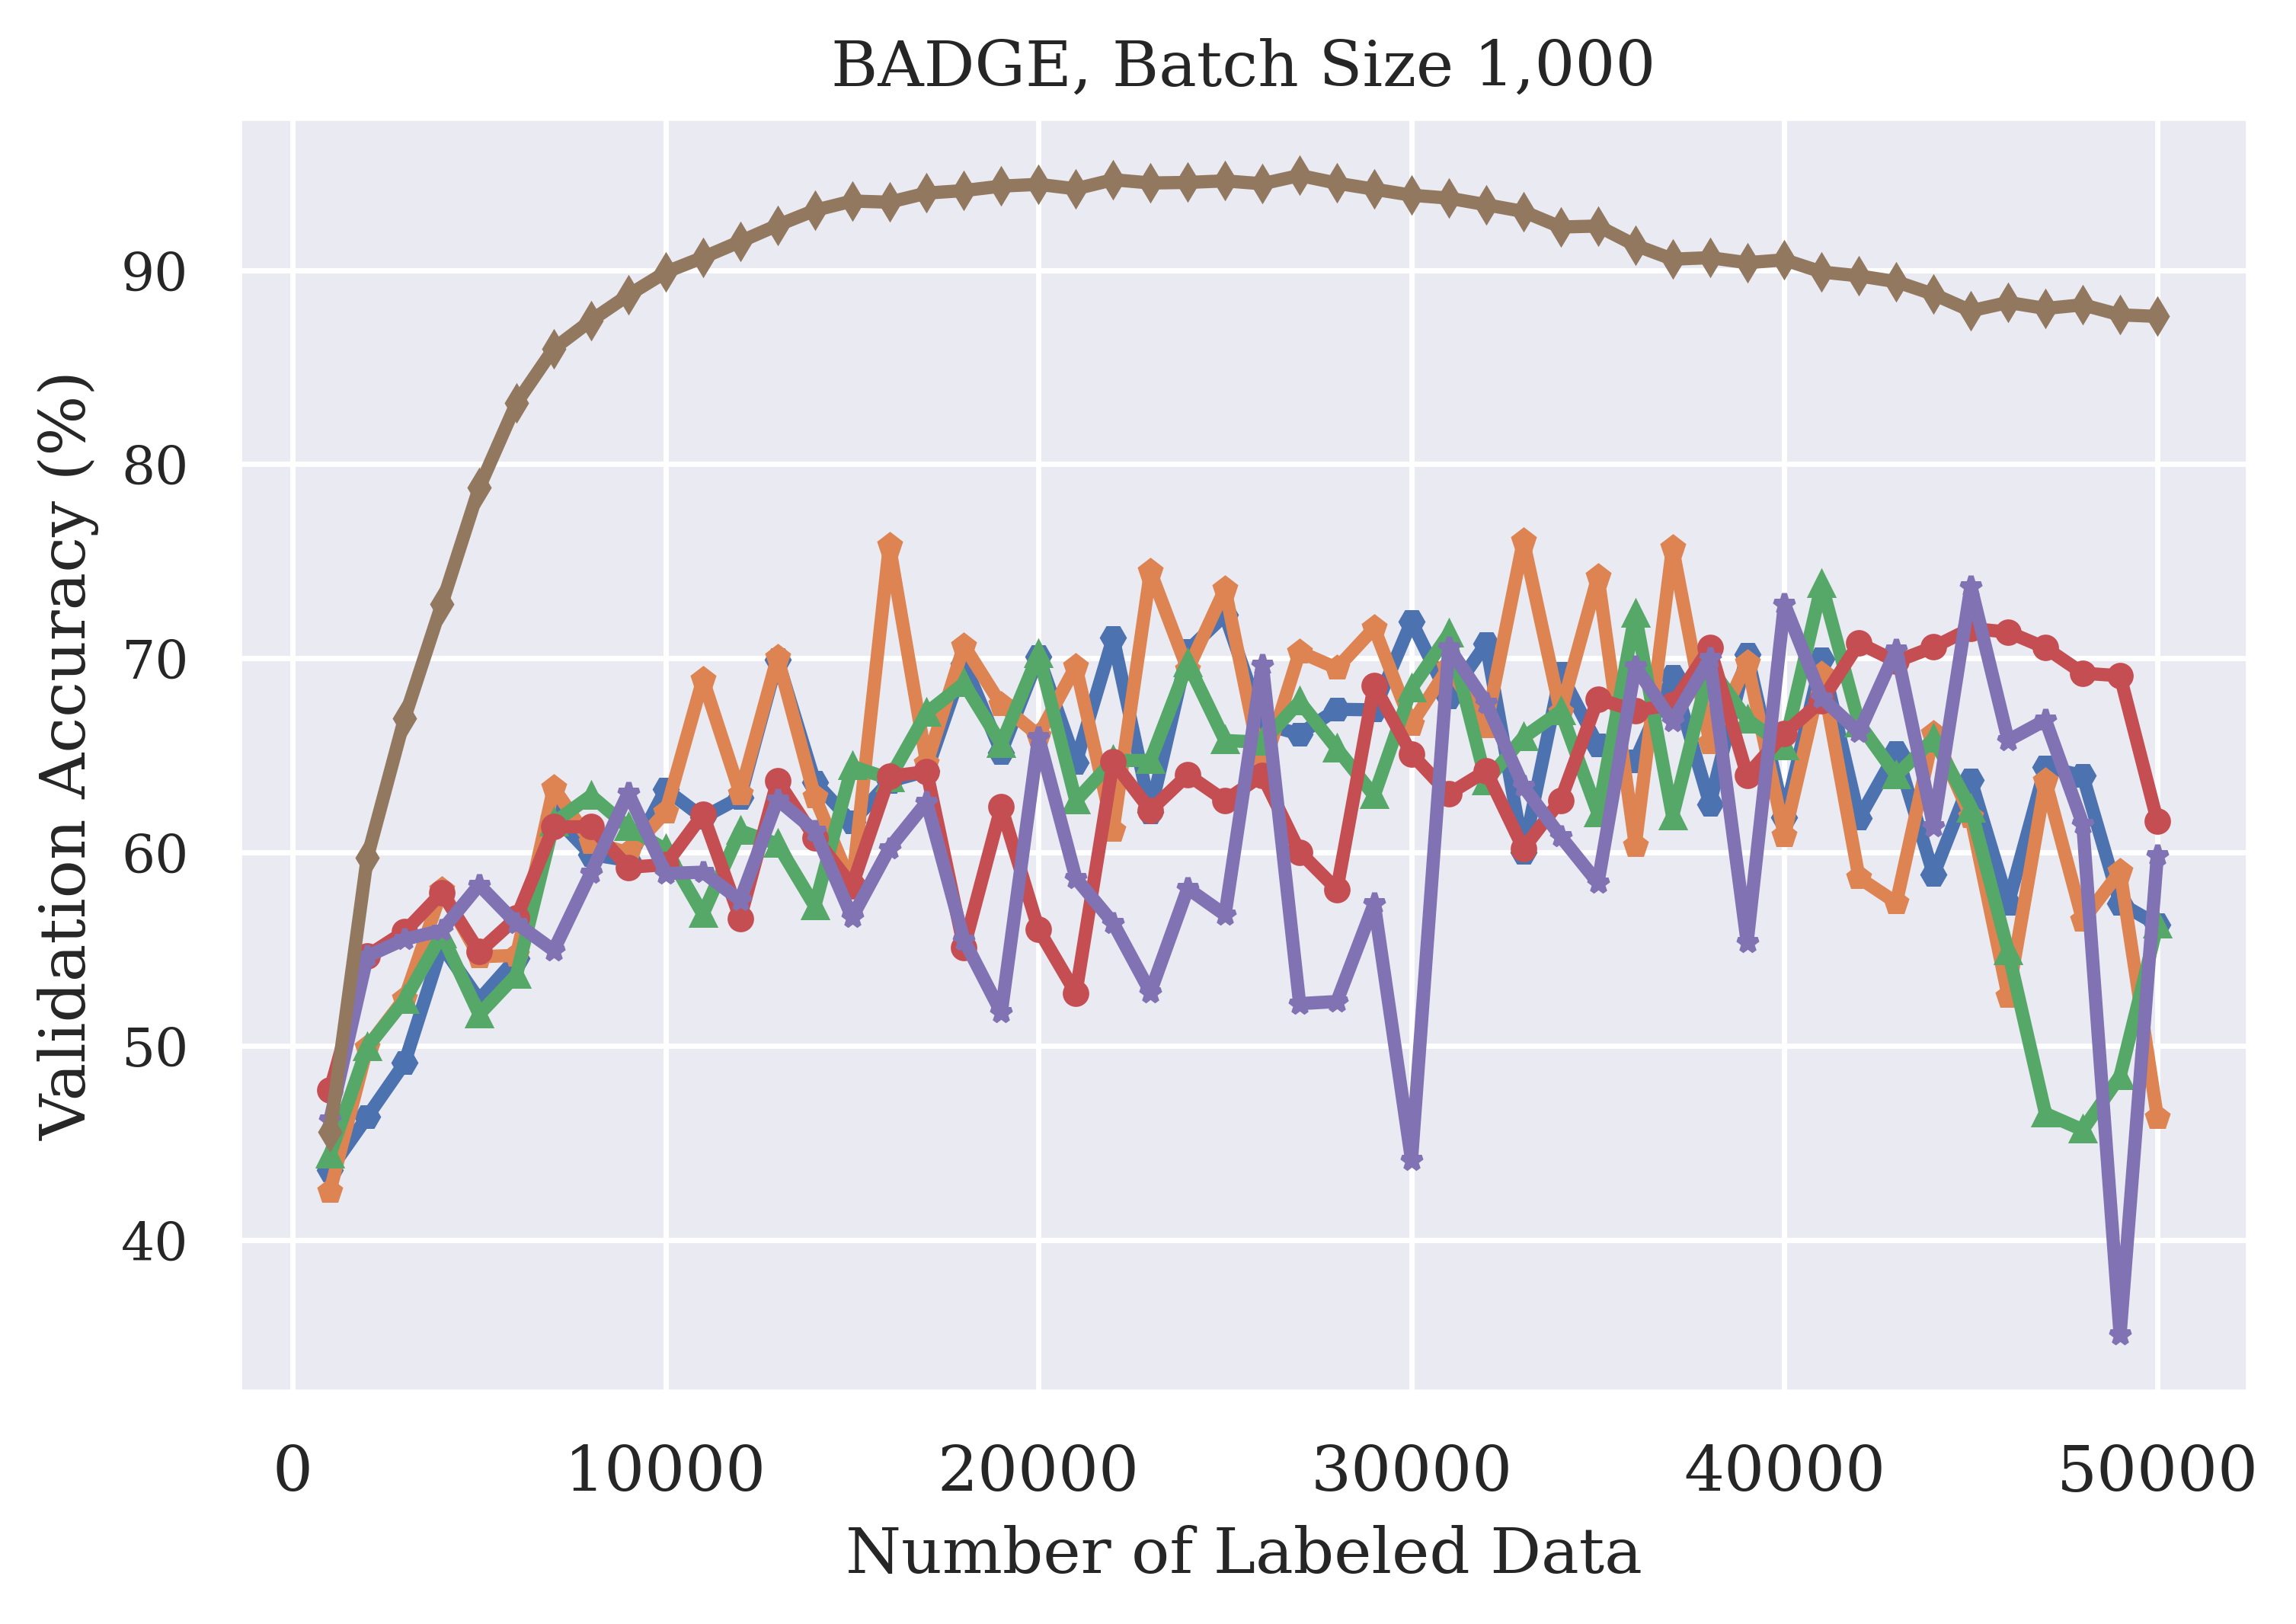
\includegraphics[width=0.32\linewidth]{images/results_CAL/badge_1000b_acc.png} \hfill
    \caption[Continual Active Learning with \gls{badge} with varying batch size]{Comparison of validation accuracy of Continual Learning and Active Learning strategies
    with batch size 1000.}
    \label{fig:Evaluation:Results:CAL:1000bAcc}
\end{figure}

% \begin{figure}[h]
%     \centering
%     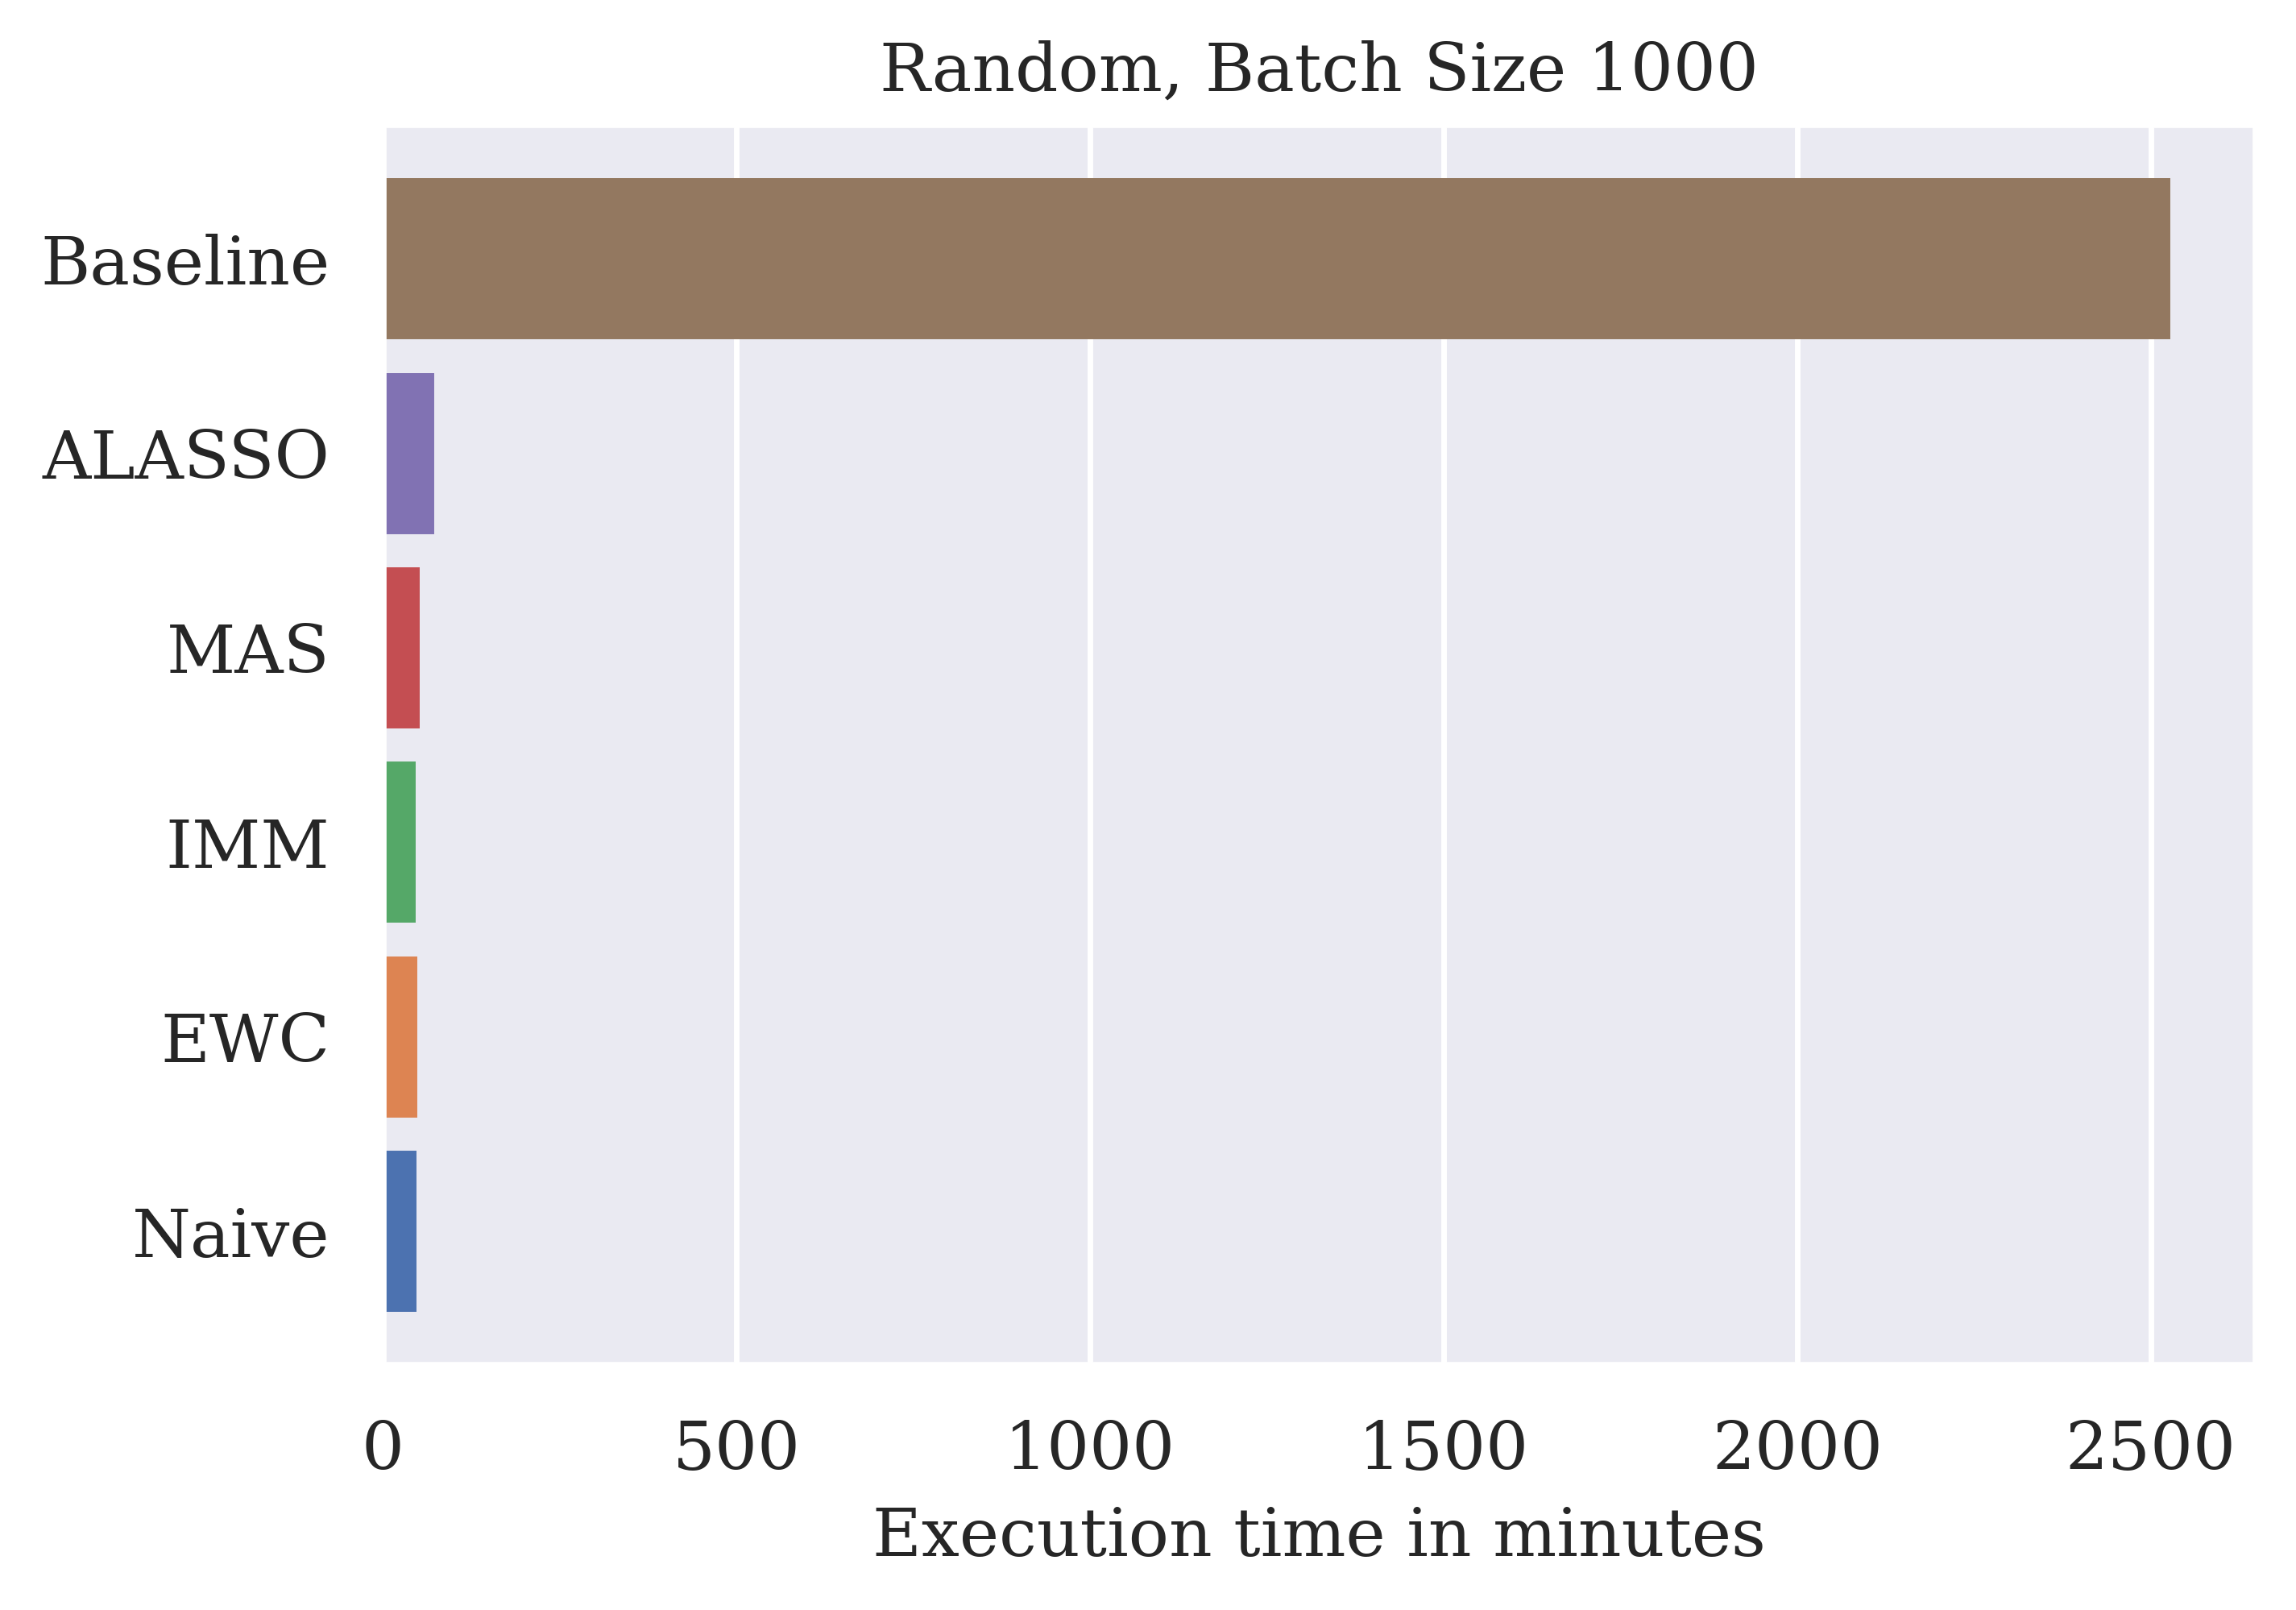
\includegraphics[width=0.32\linewidth]{images/results_CAL/random_1000b_time.png} \hfill
%     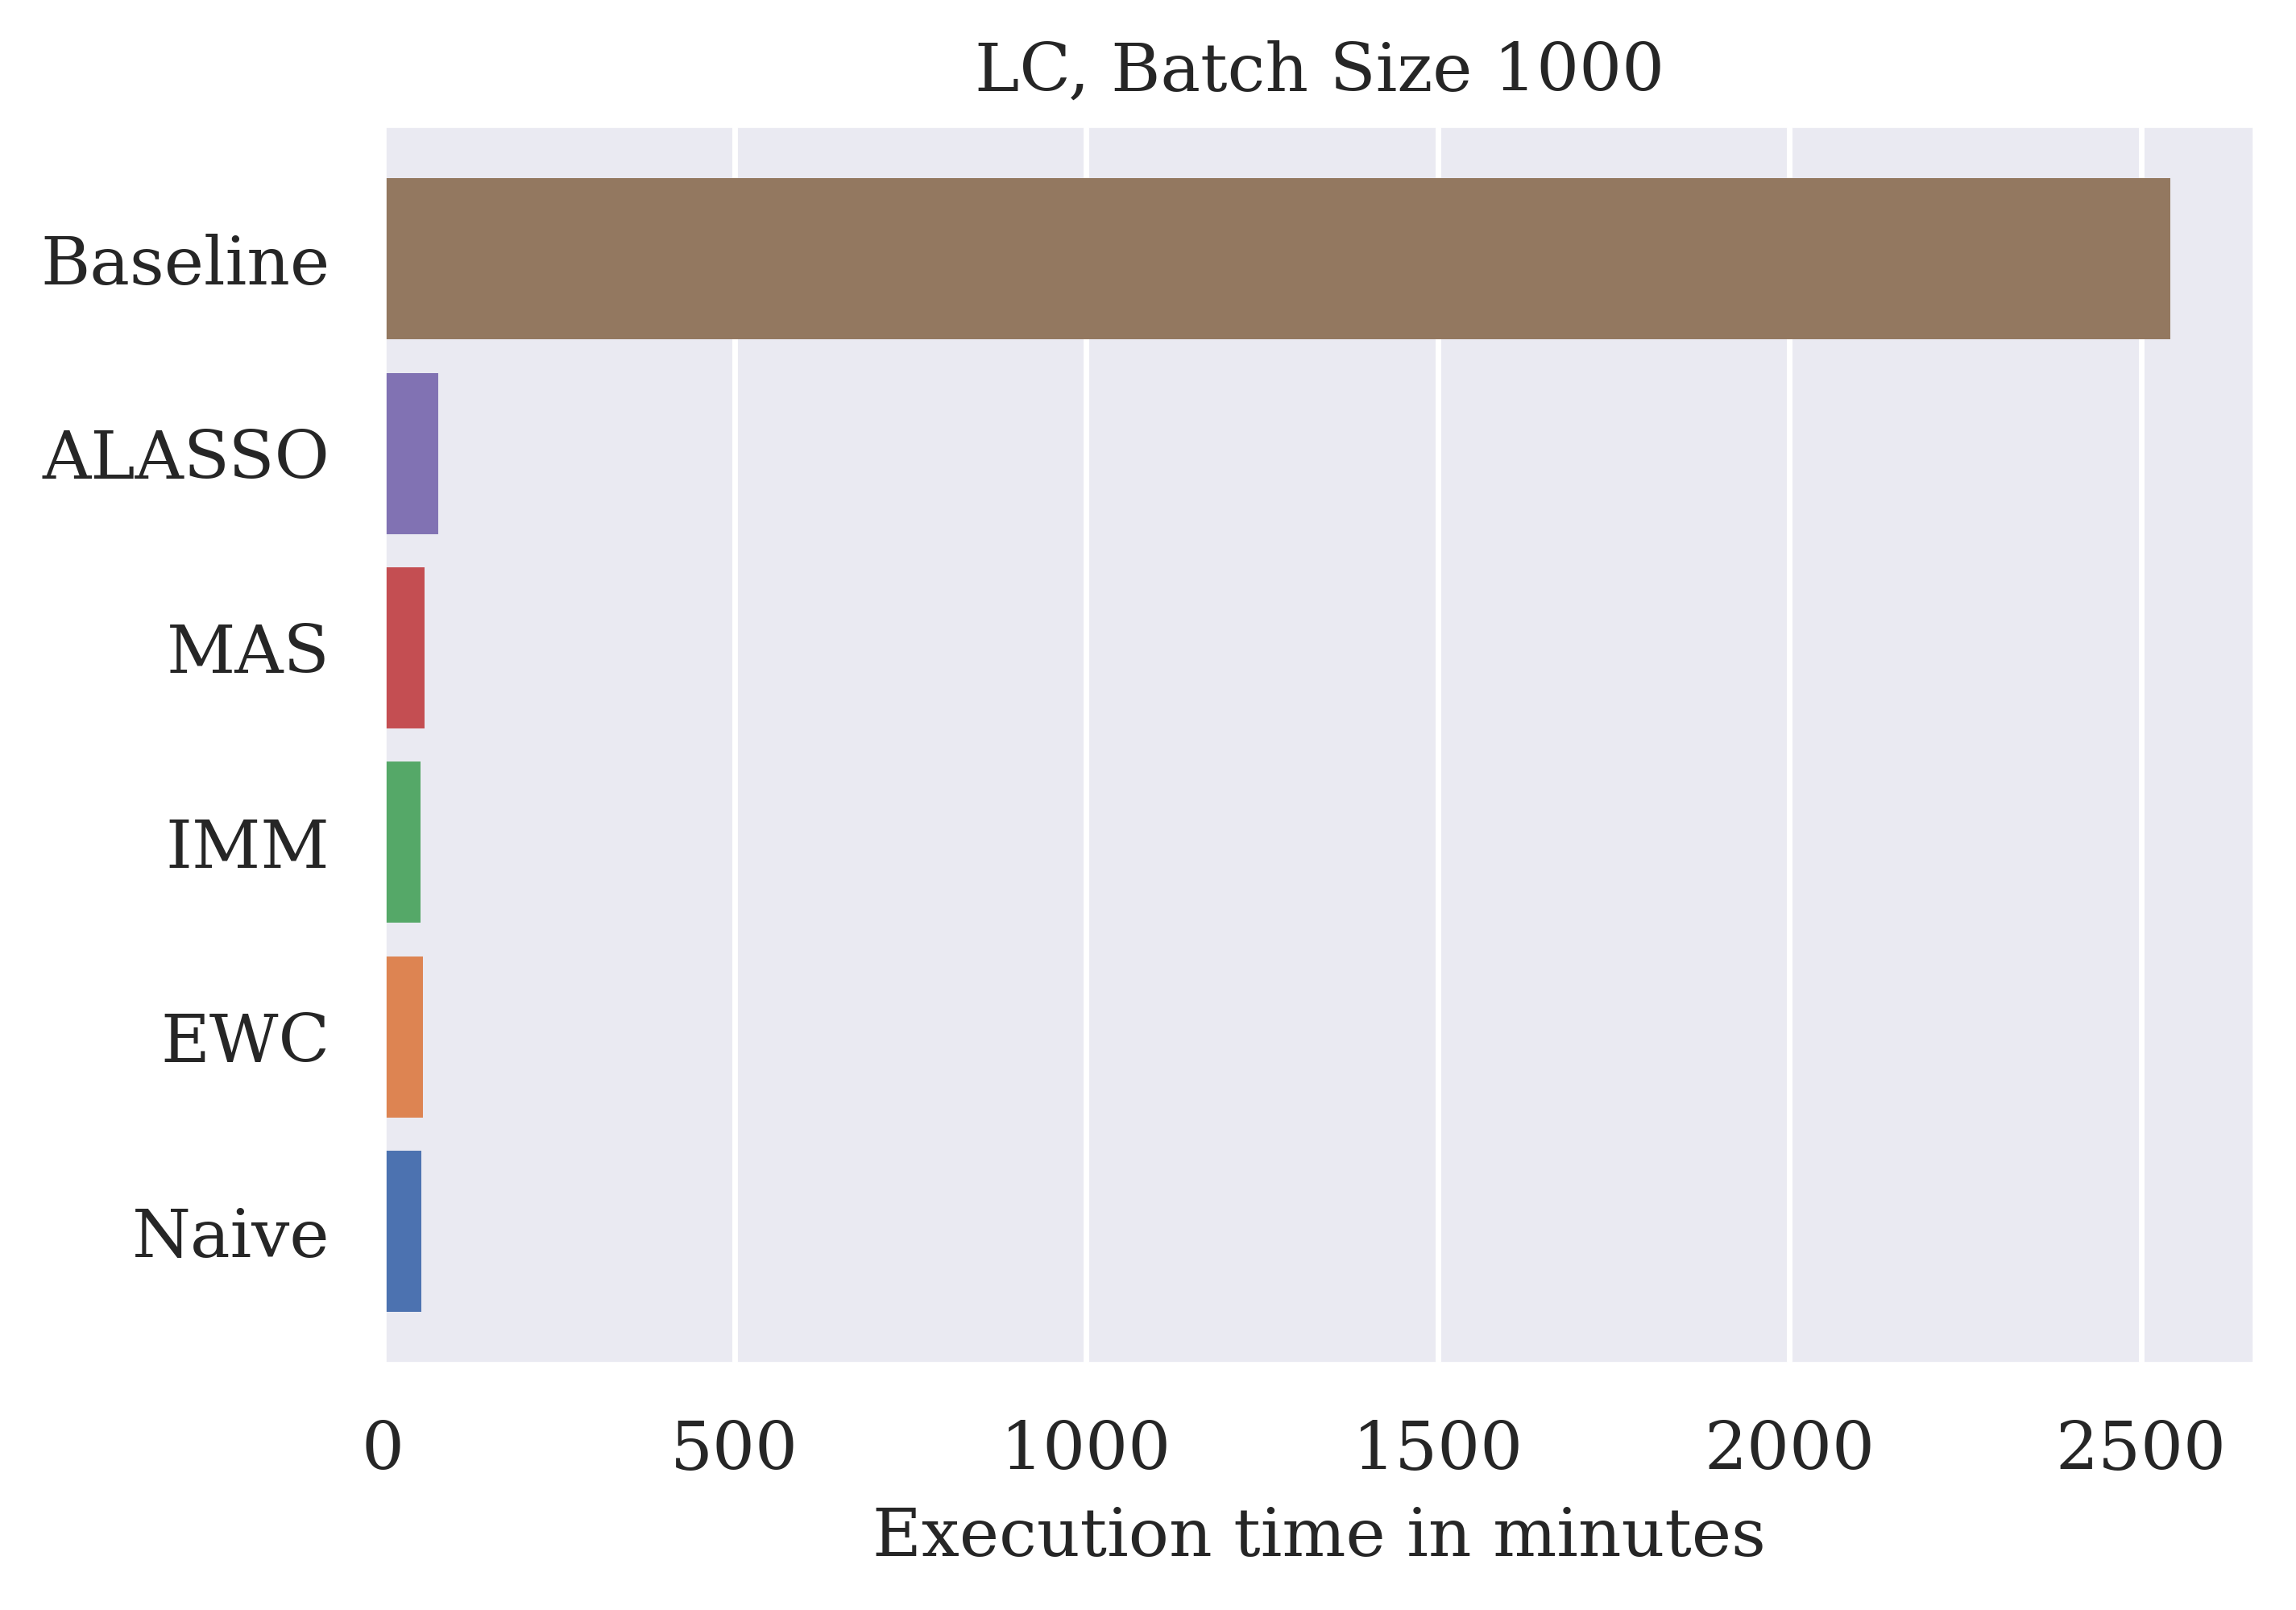
\includegraphics[width=0.32\linewidth]{images/results_CAL/lc_1000b_time.png} \hfill
%     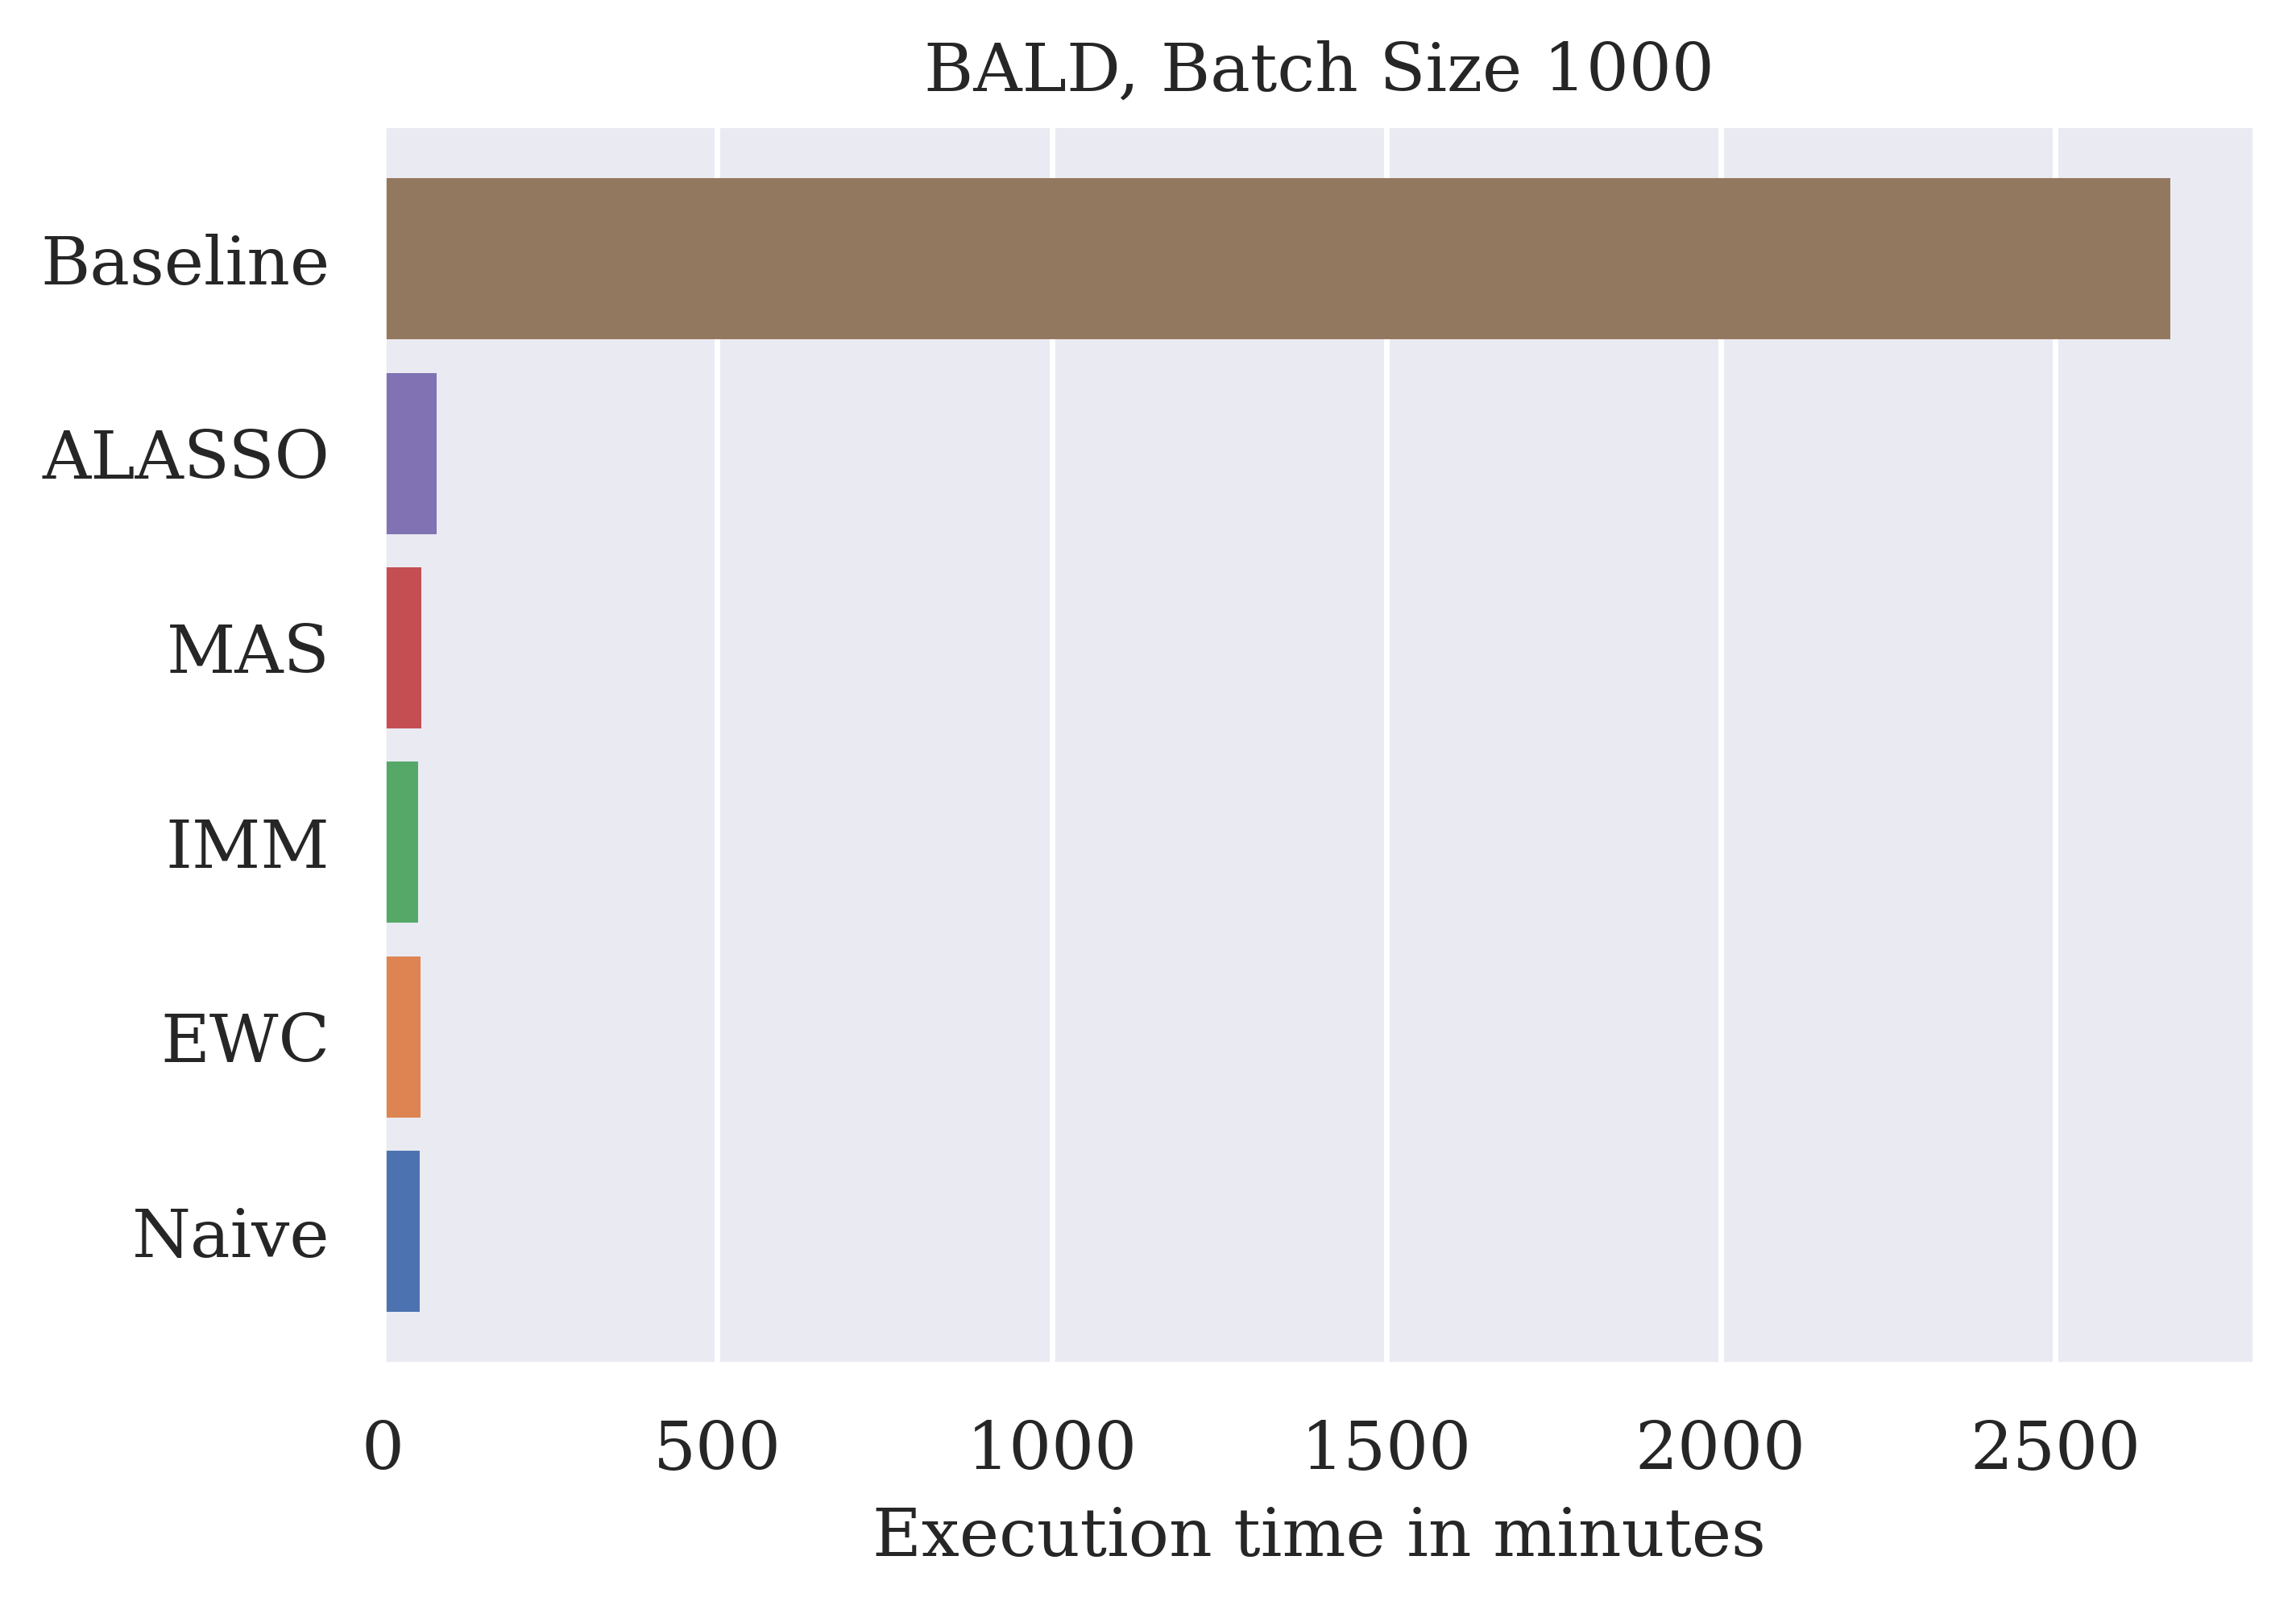
\includegraphics[width=0.32\linewidth]{images/results_CAL/bald_1000b_time.png}
%     \\[\smallskipamount]
%     \hfill 
%     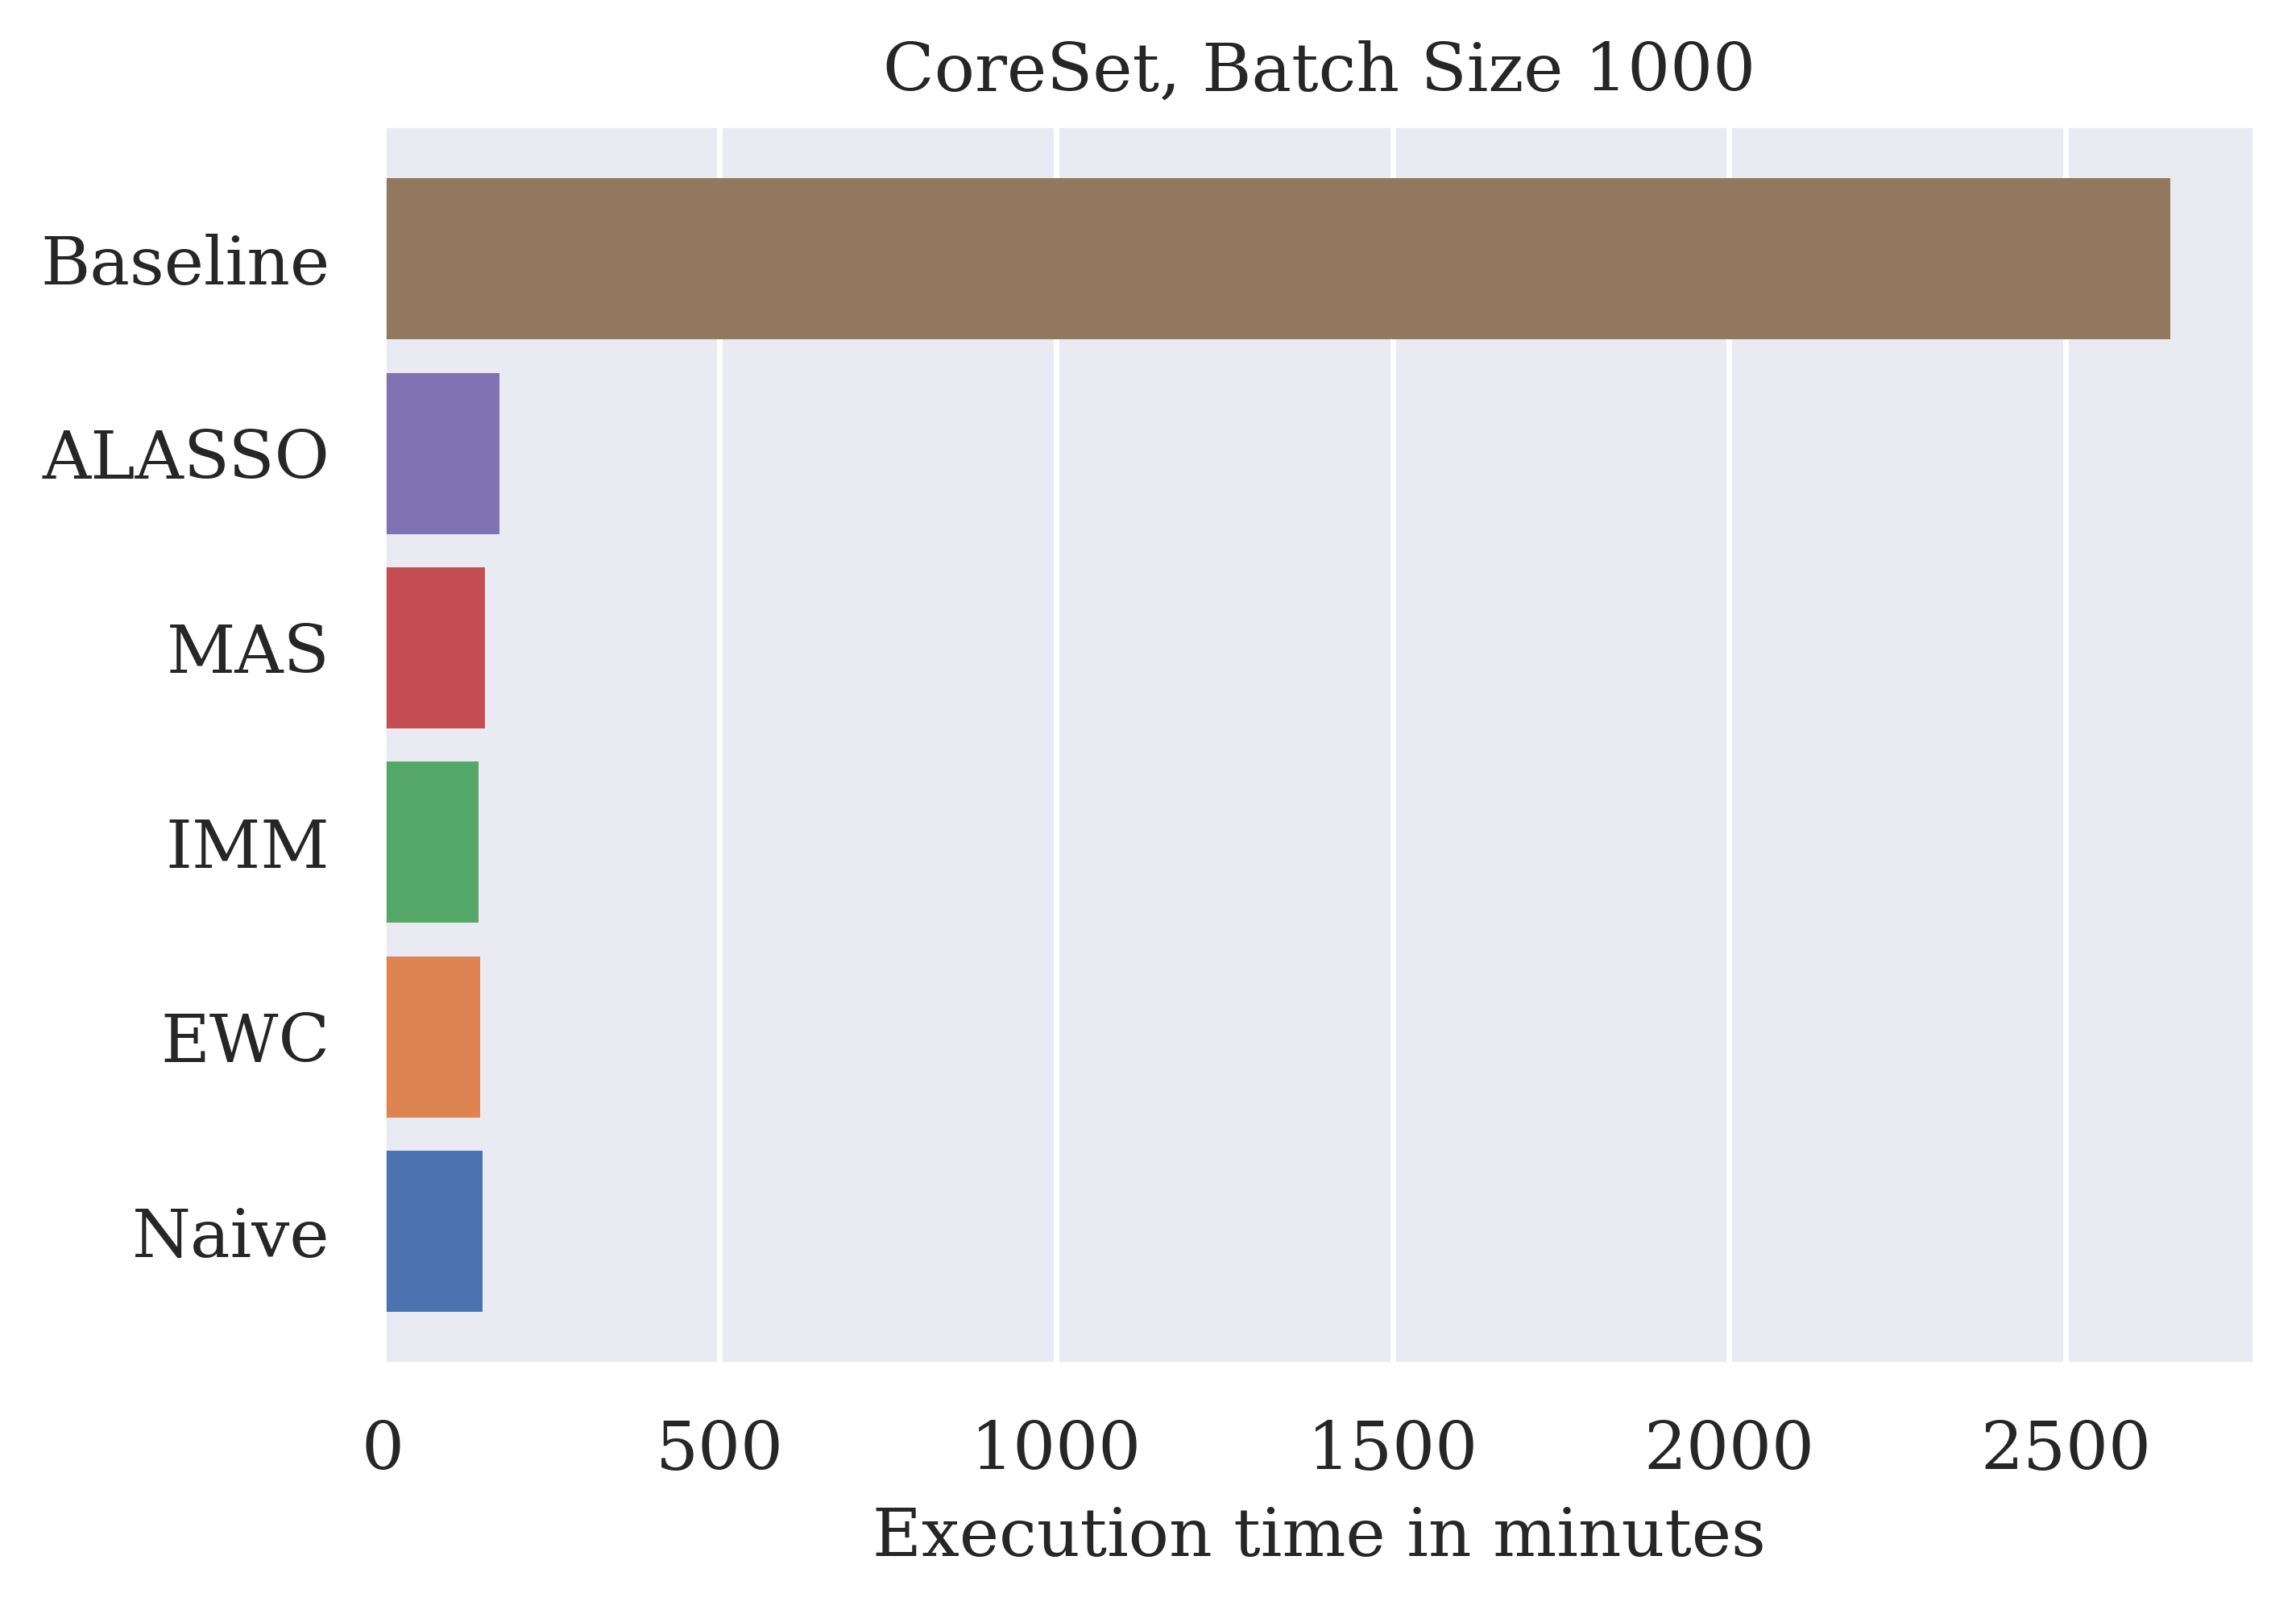
\includegraphics[width=0.32\linewidth]{images/results_CAL/coreset_1000b_time.png} \hfill
%     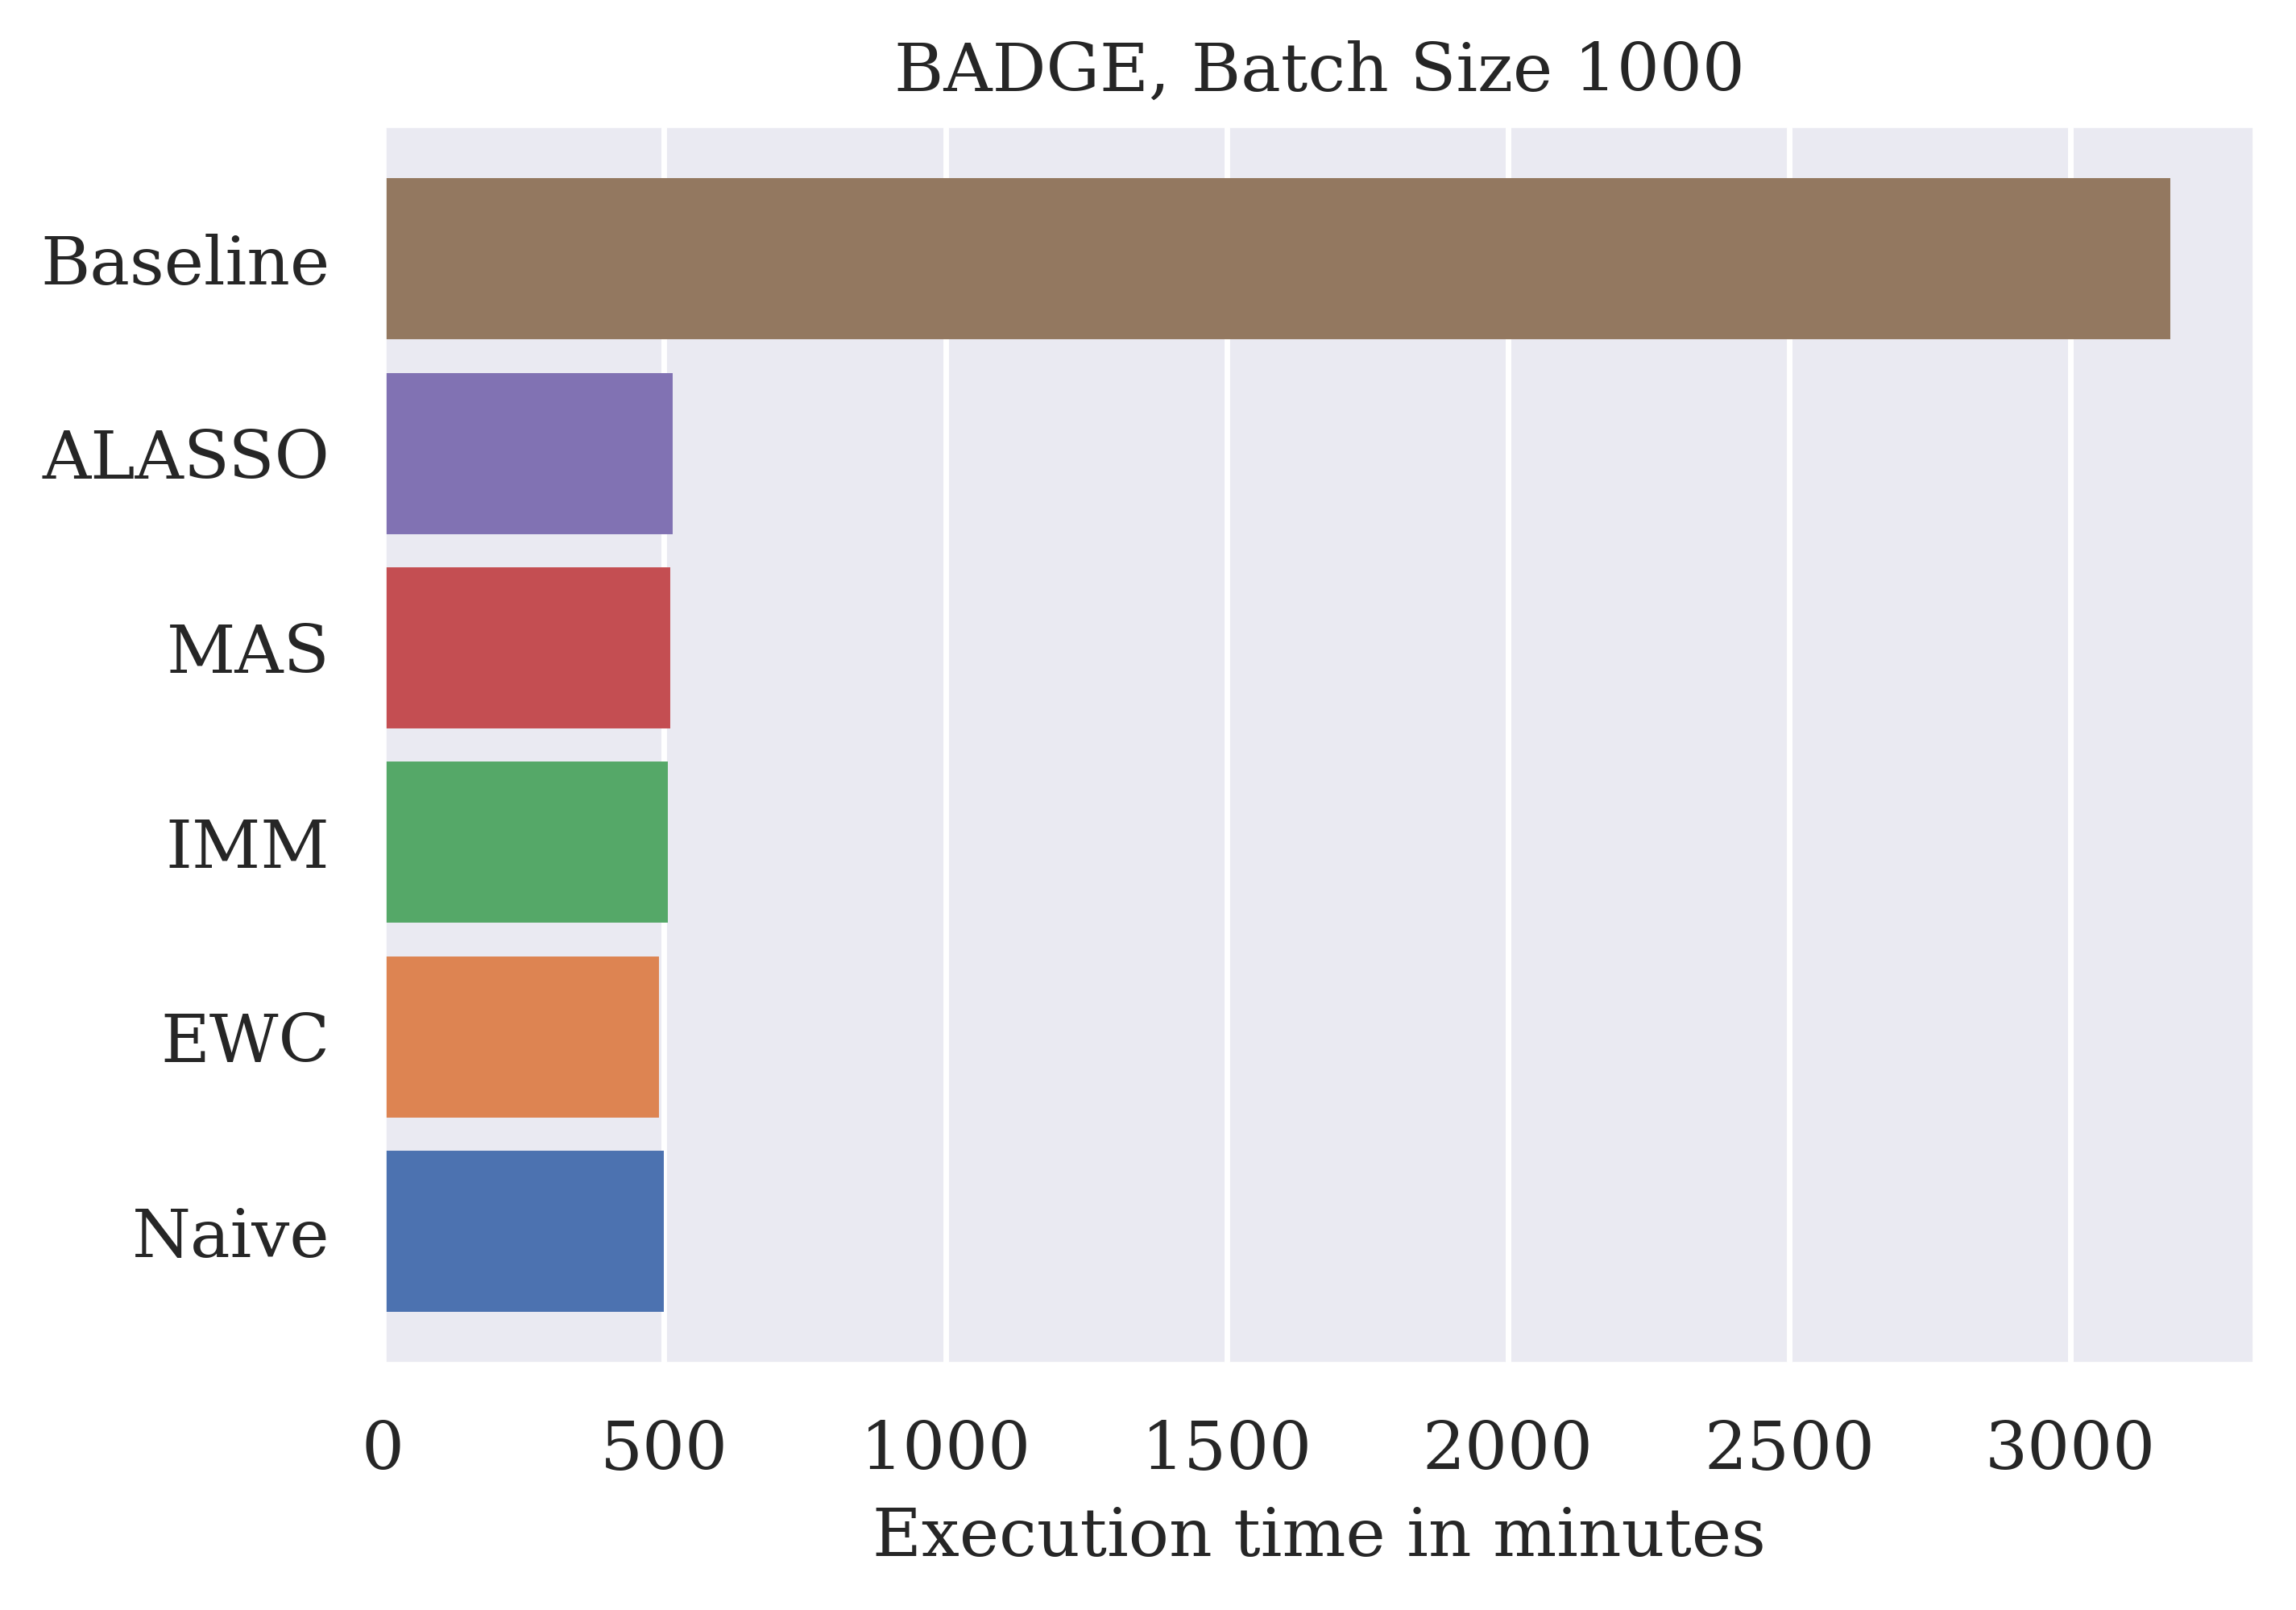
\includegraphics[width=0.32\linewidth]{images/results_CAL/badge_1000b_time.png} \hfill
%     \caption{Comparison of execution time of Continual Learning and Active Learning strategies
%     with batch size 1000.}
%     \label{fig:Evaluation:Results:CAL:1000bTime}
% \end{figure}

\begin{table}[h]
    \centering
    \begin{tabular}{c | c c c c c } 
         & Random & \gls{lc} & \gls{bald} & CoreSet & \gls{badge}\\ 
        \hline 
        Baseline & 2522 & 2536 & 2549 & 2650 & 3171 \\
        \hline
        Naive & 44 & 50 & 50 & 144 & 493 \\
        \gls{ewc} & 44 & 53 & 51 & 140 & 486\\
        \gls{imm} & 42 & 49 & 48 & 137 & 501\\
        \gls{mas} & 48 & 55 & 53 & 147 & 505\\
        \gls{alasso} & 68 & 75 & 75 & 168 & 509\\
    \end{tabular}
    \caption{Comparison of execution time of regularization-based continual learning strategies
    with batch size 1000.}
    \label{fig:Evaluation:Results:CAL:1000bTimeTable}
\end{table}


\begin{figure}[h]
    \centering
    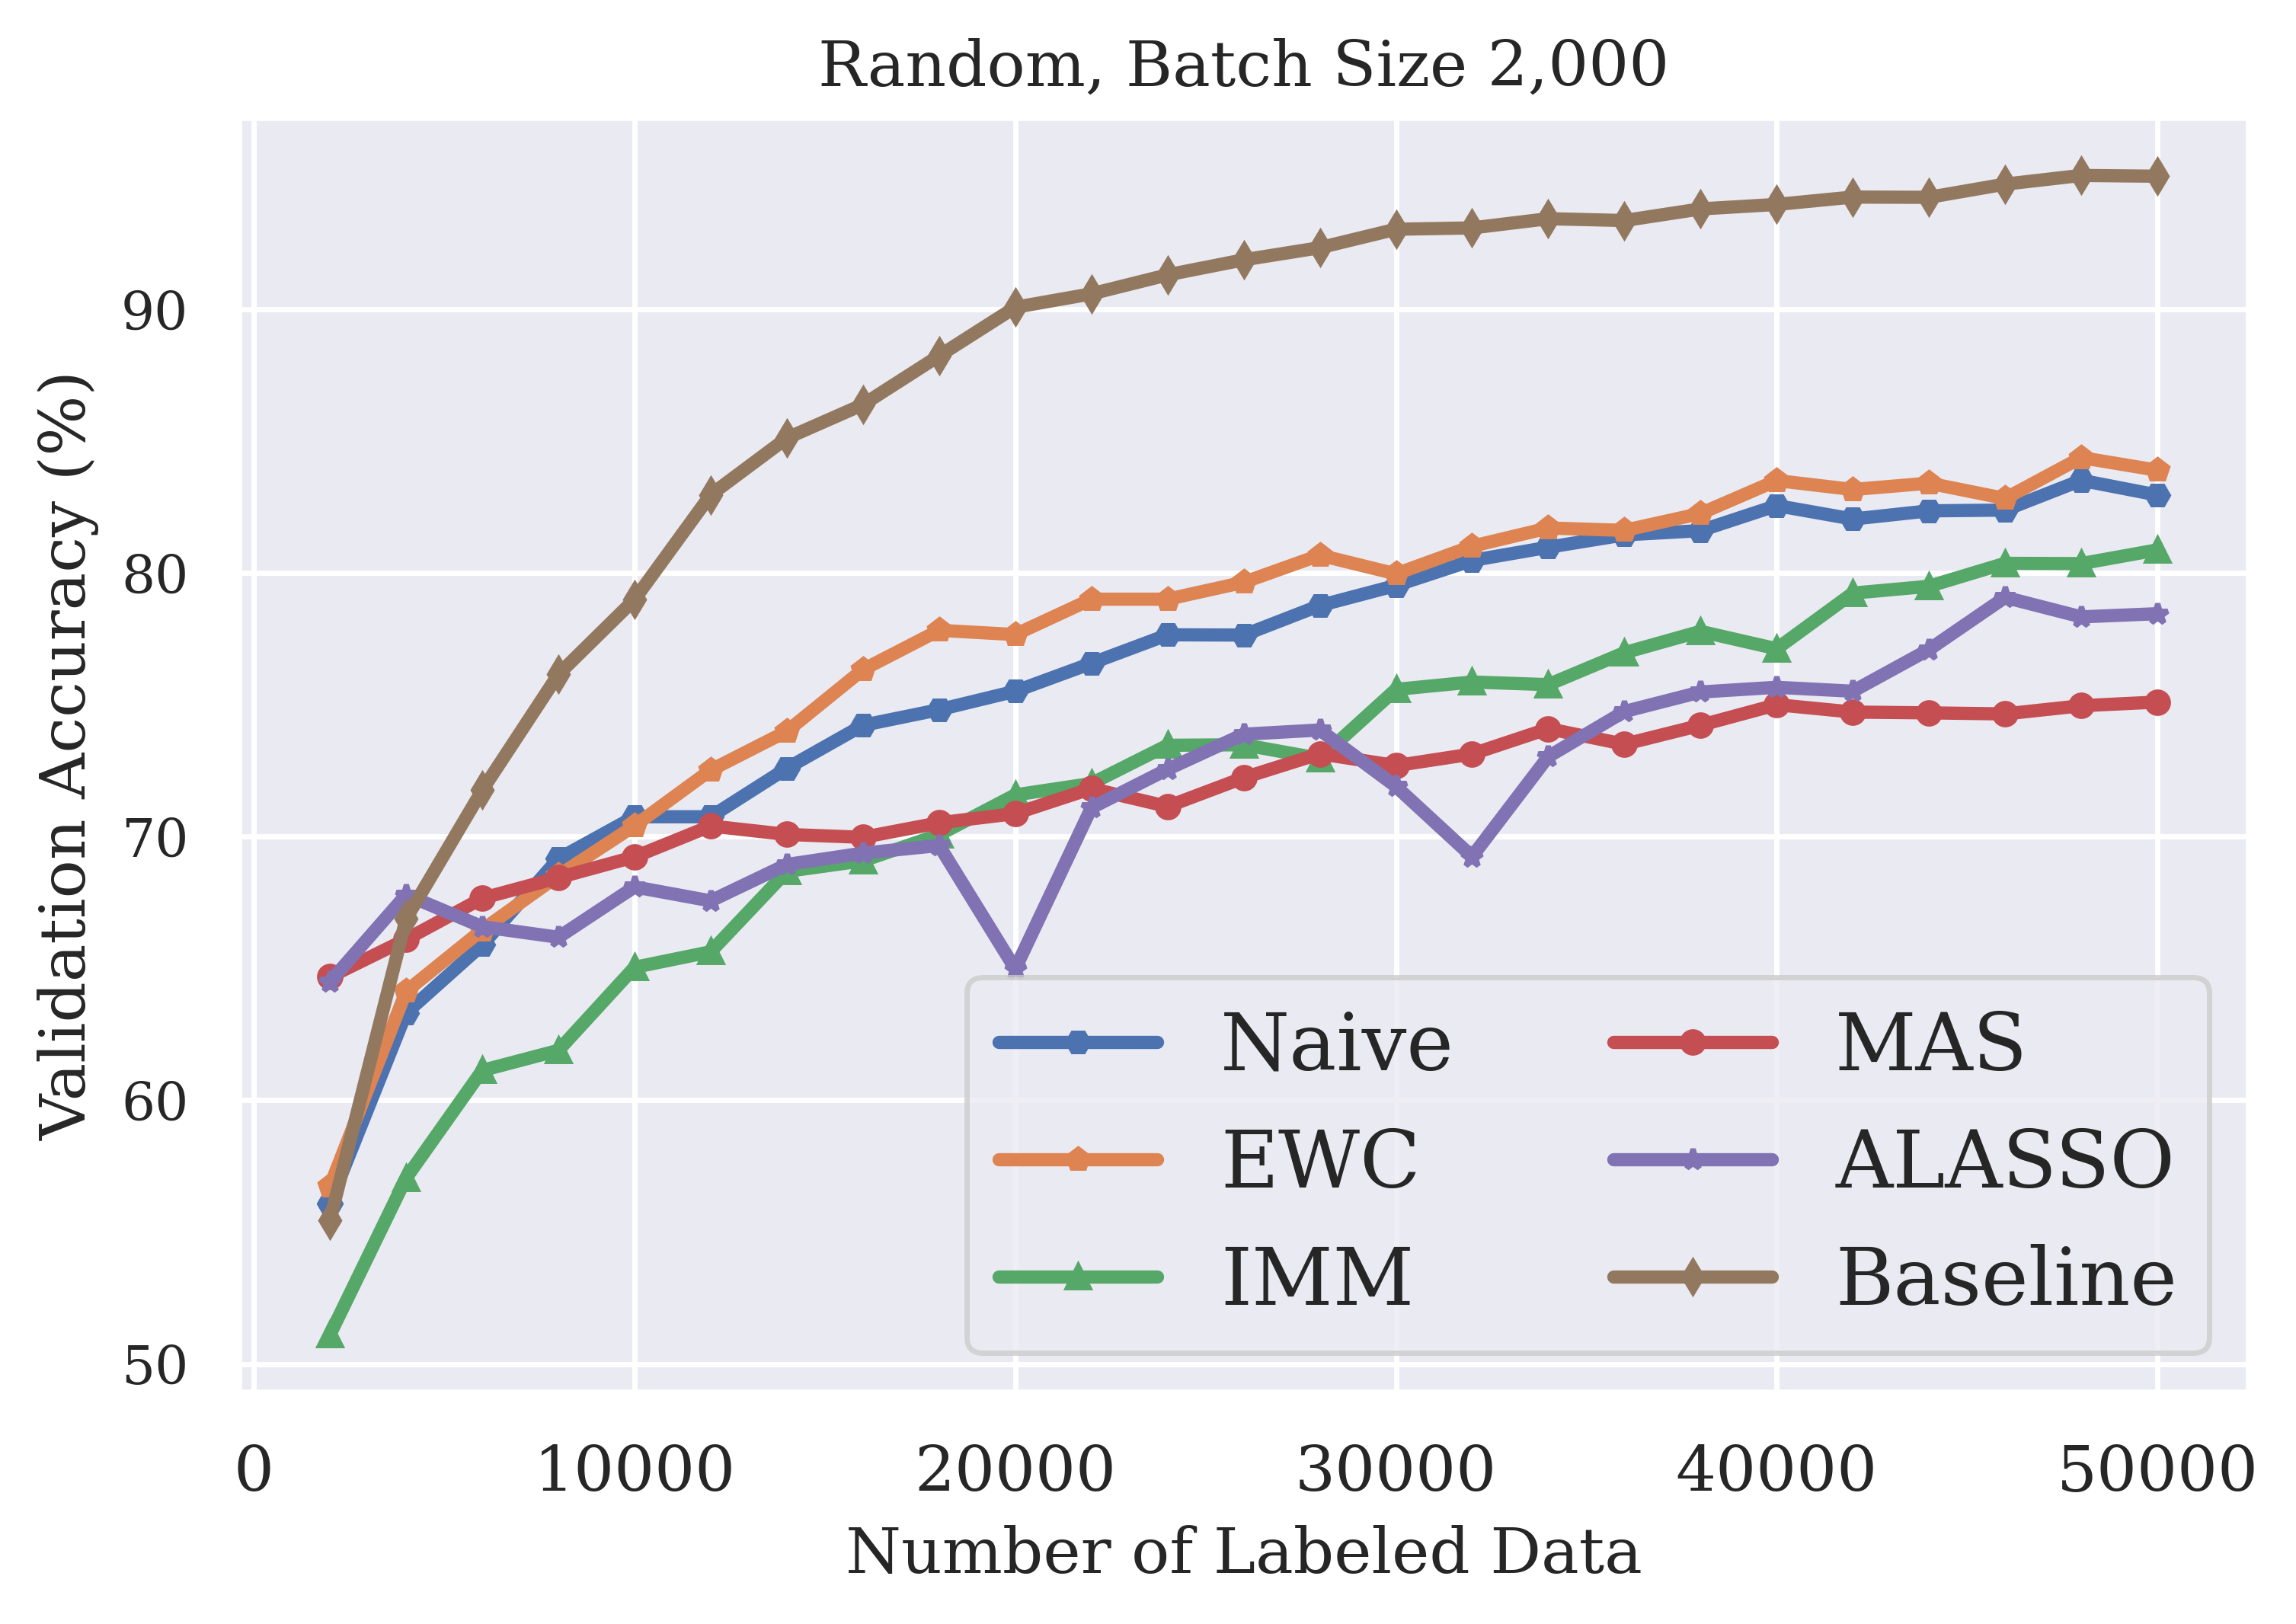
\includegraphics[width=0.32\linewidth]{images/results_CAL/random_2000b_acc.png} \hfill
    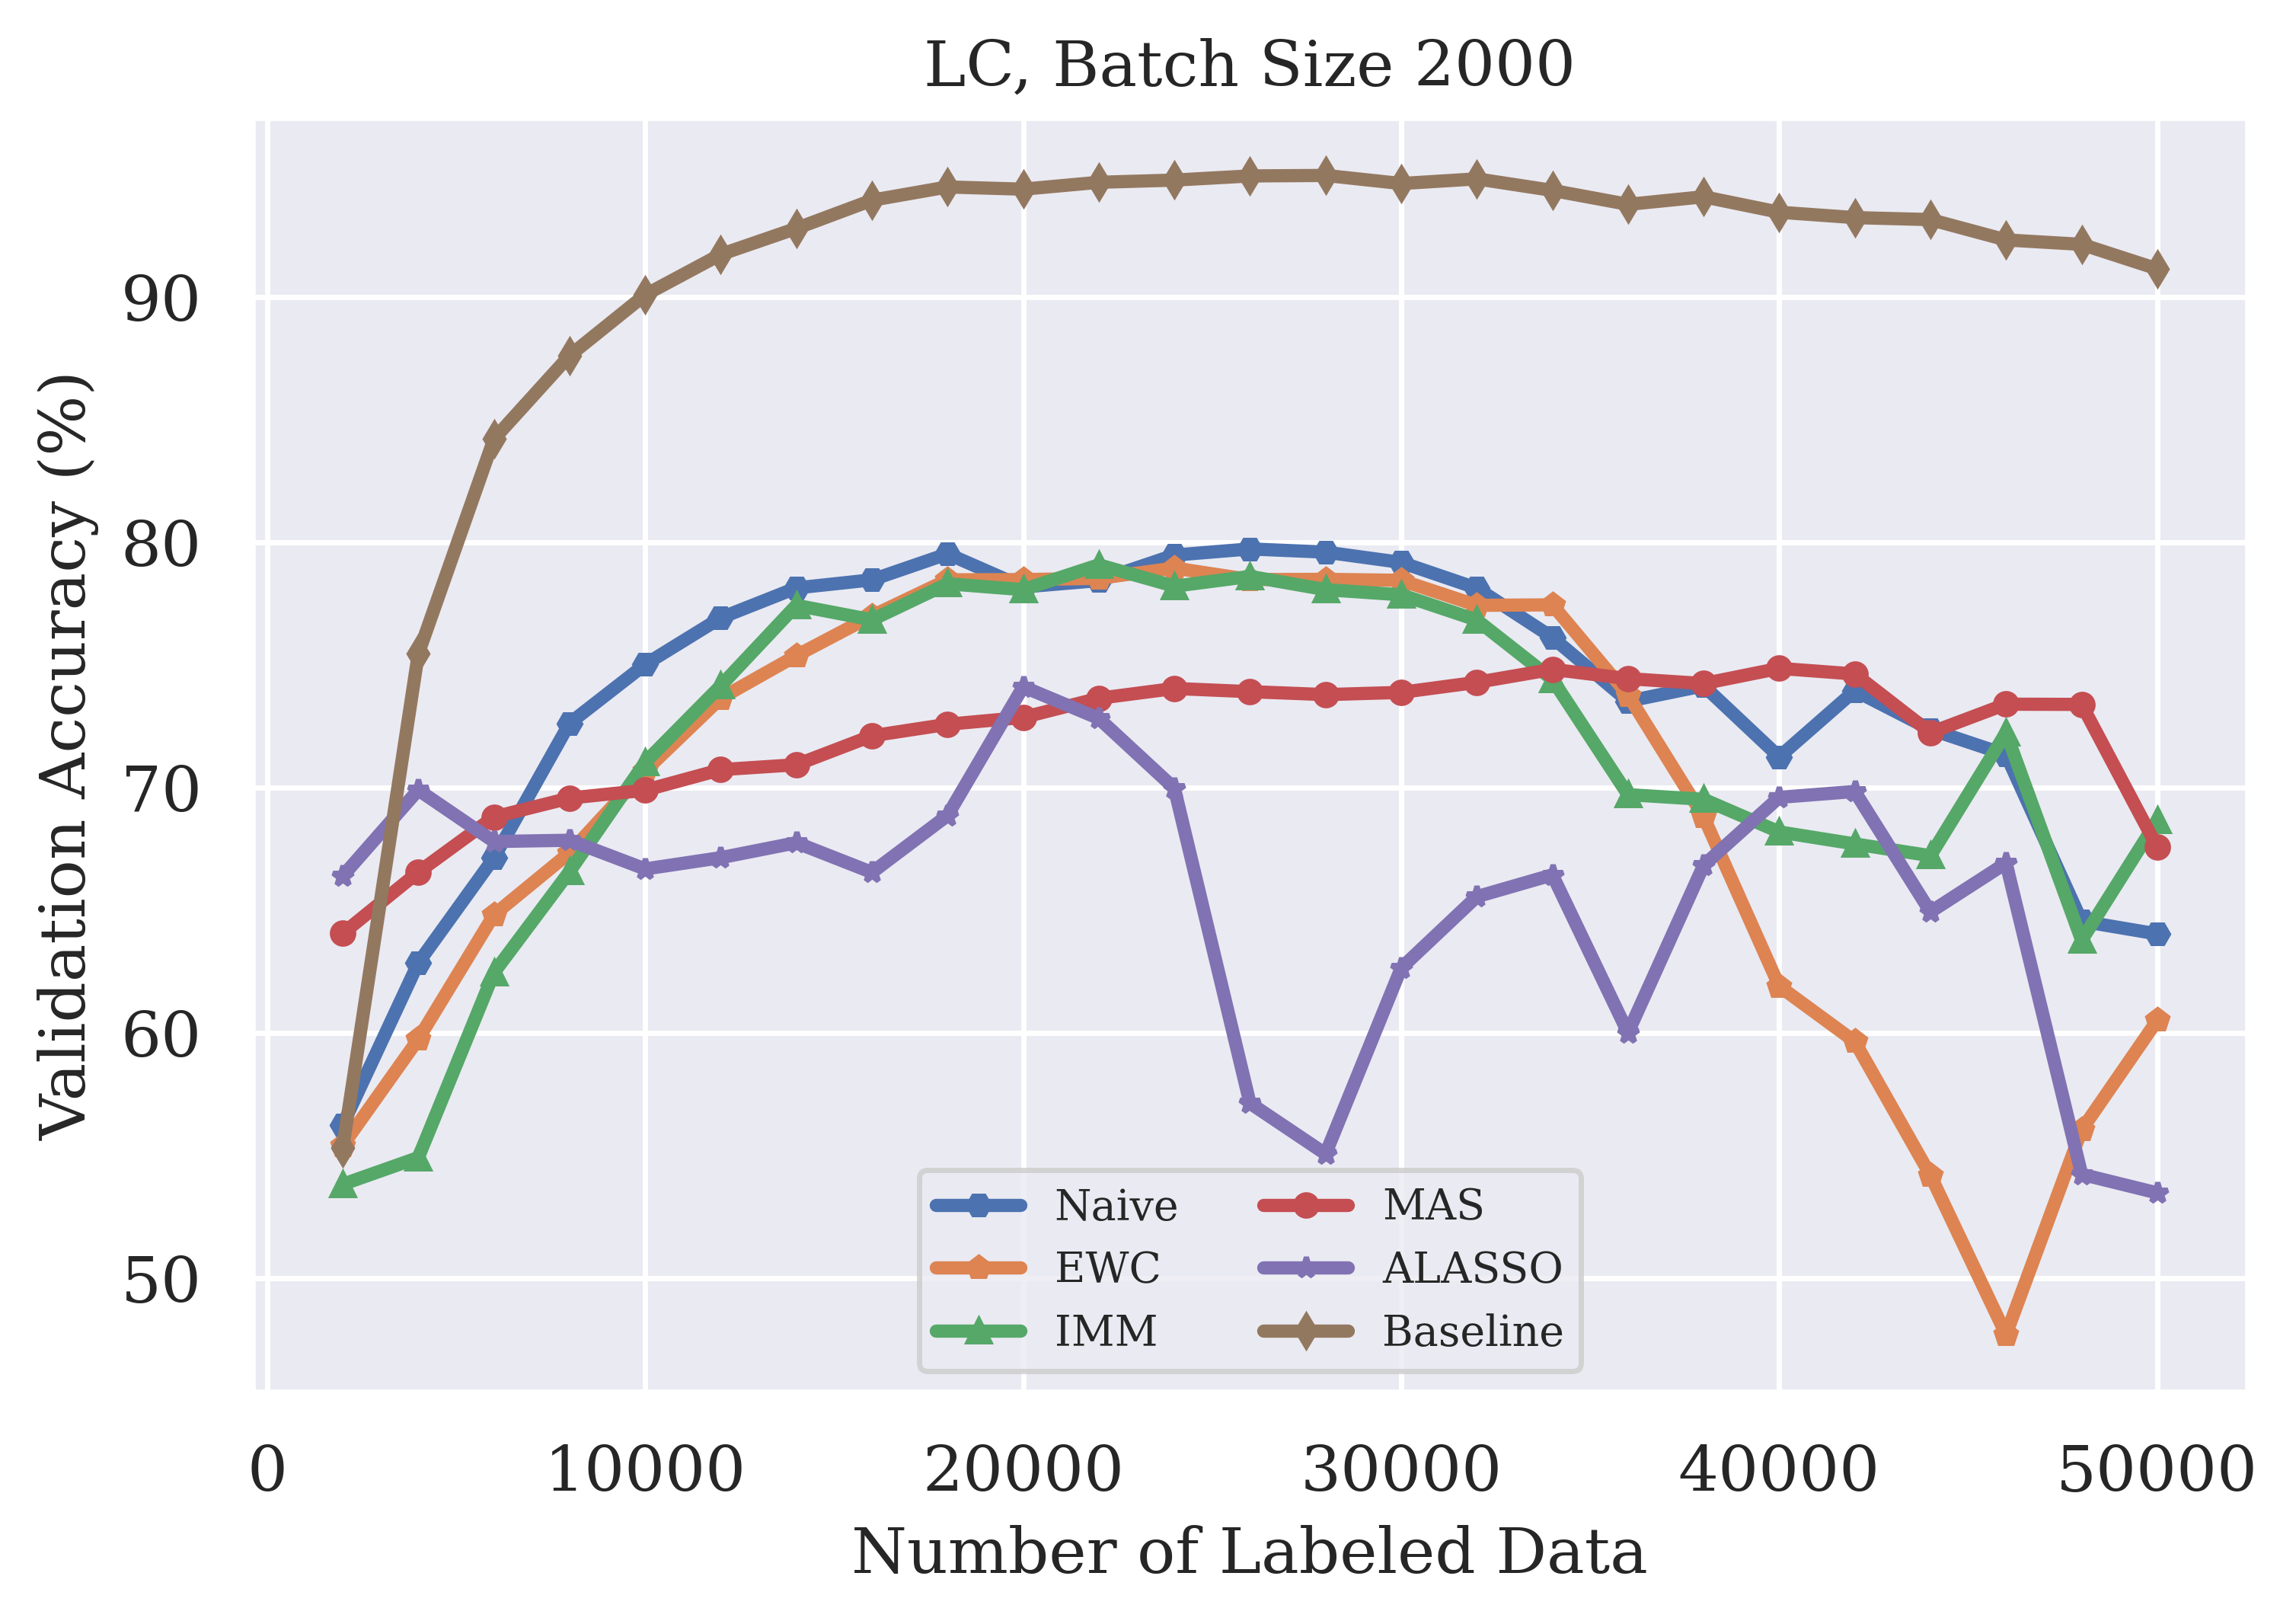
\includegraphics[width=0.32\linewidth]{images/results_CAL/lc_2000b_acc.png} \hfill
    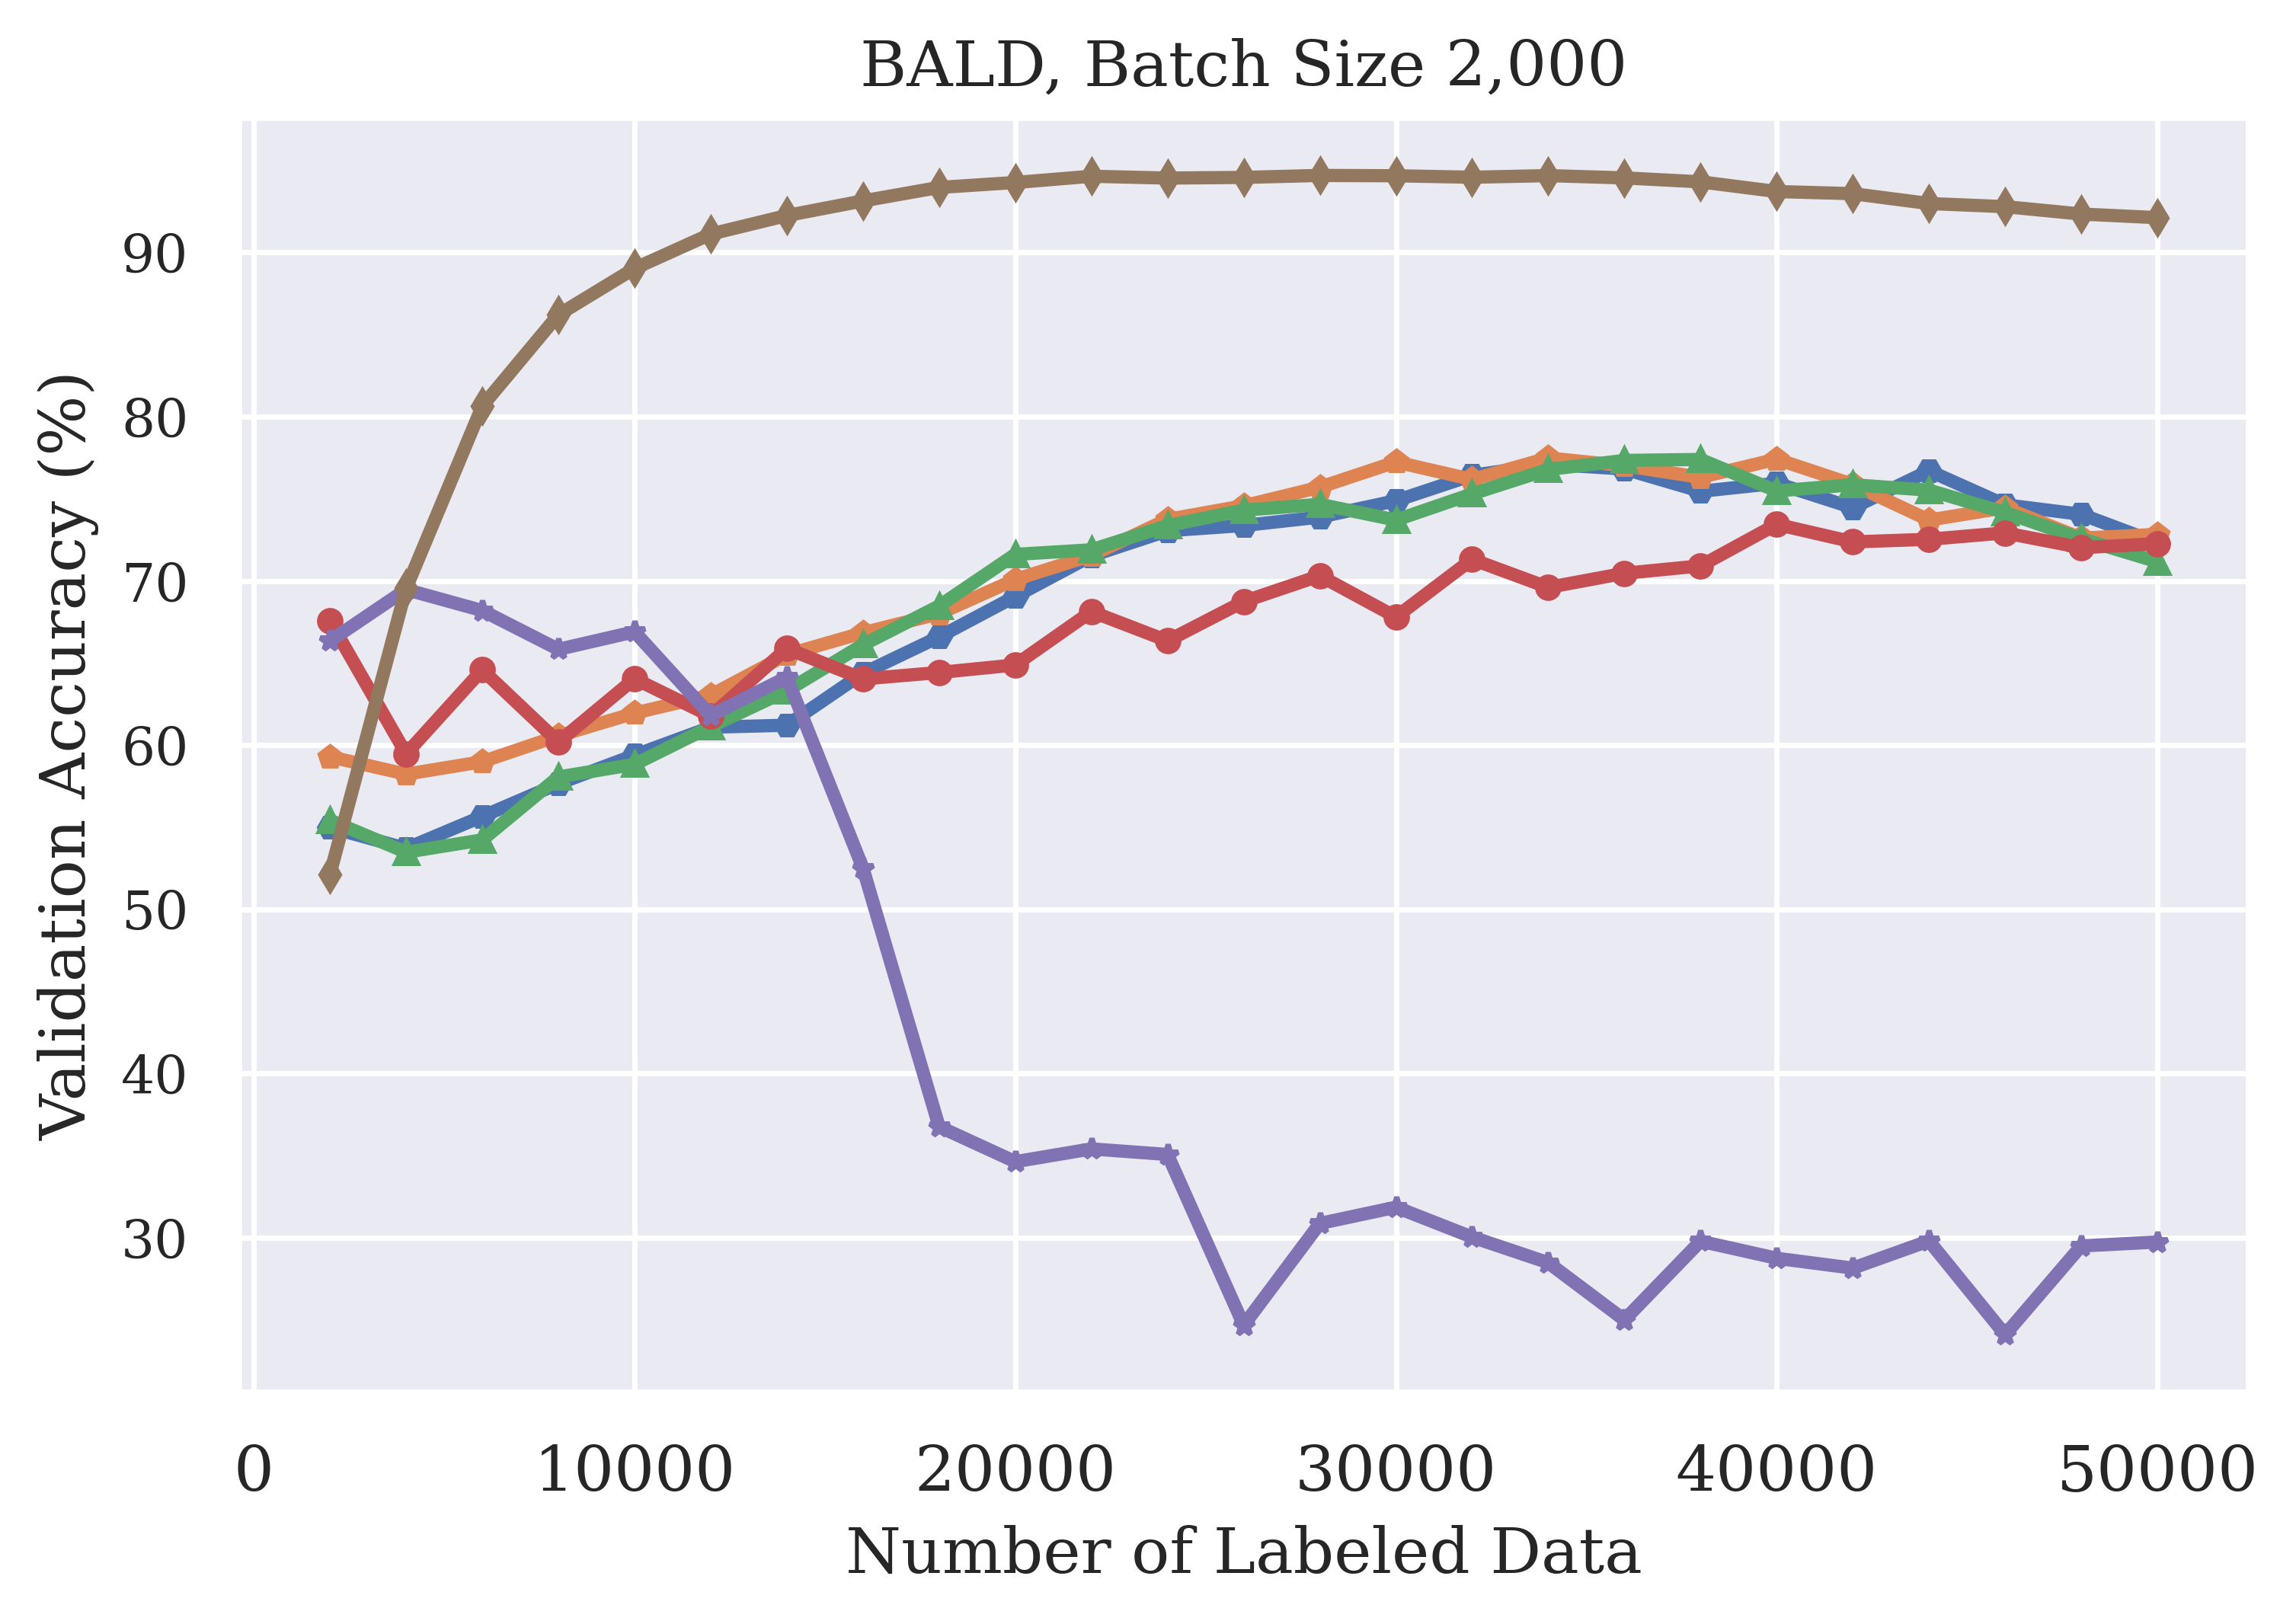
\includegraphics[width=0.32\linewidth]{images/results_CAL/bald_2000b_acc.png}
    \\[\smallskipamount]
    \hfill 
    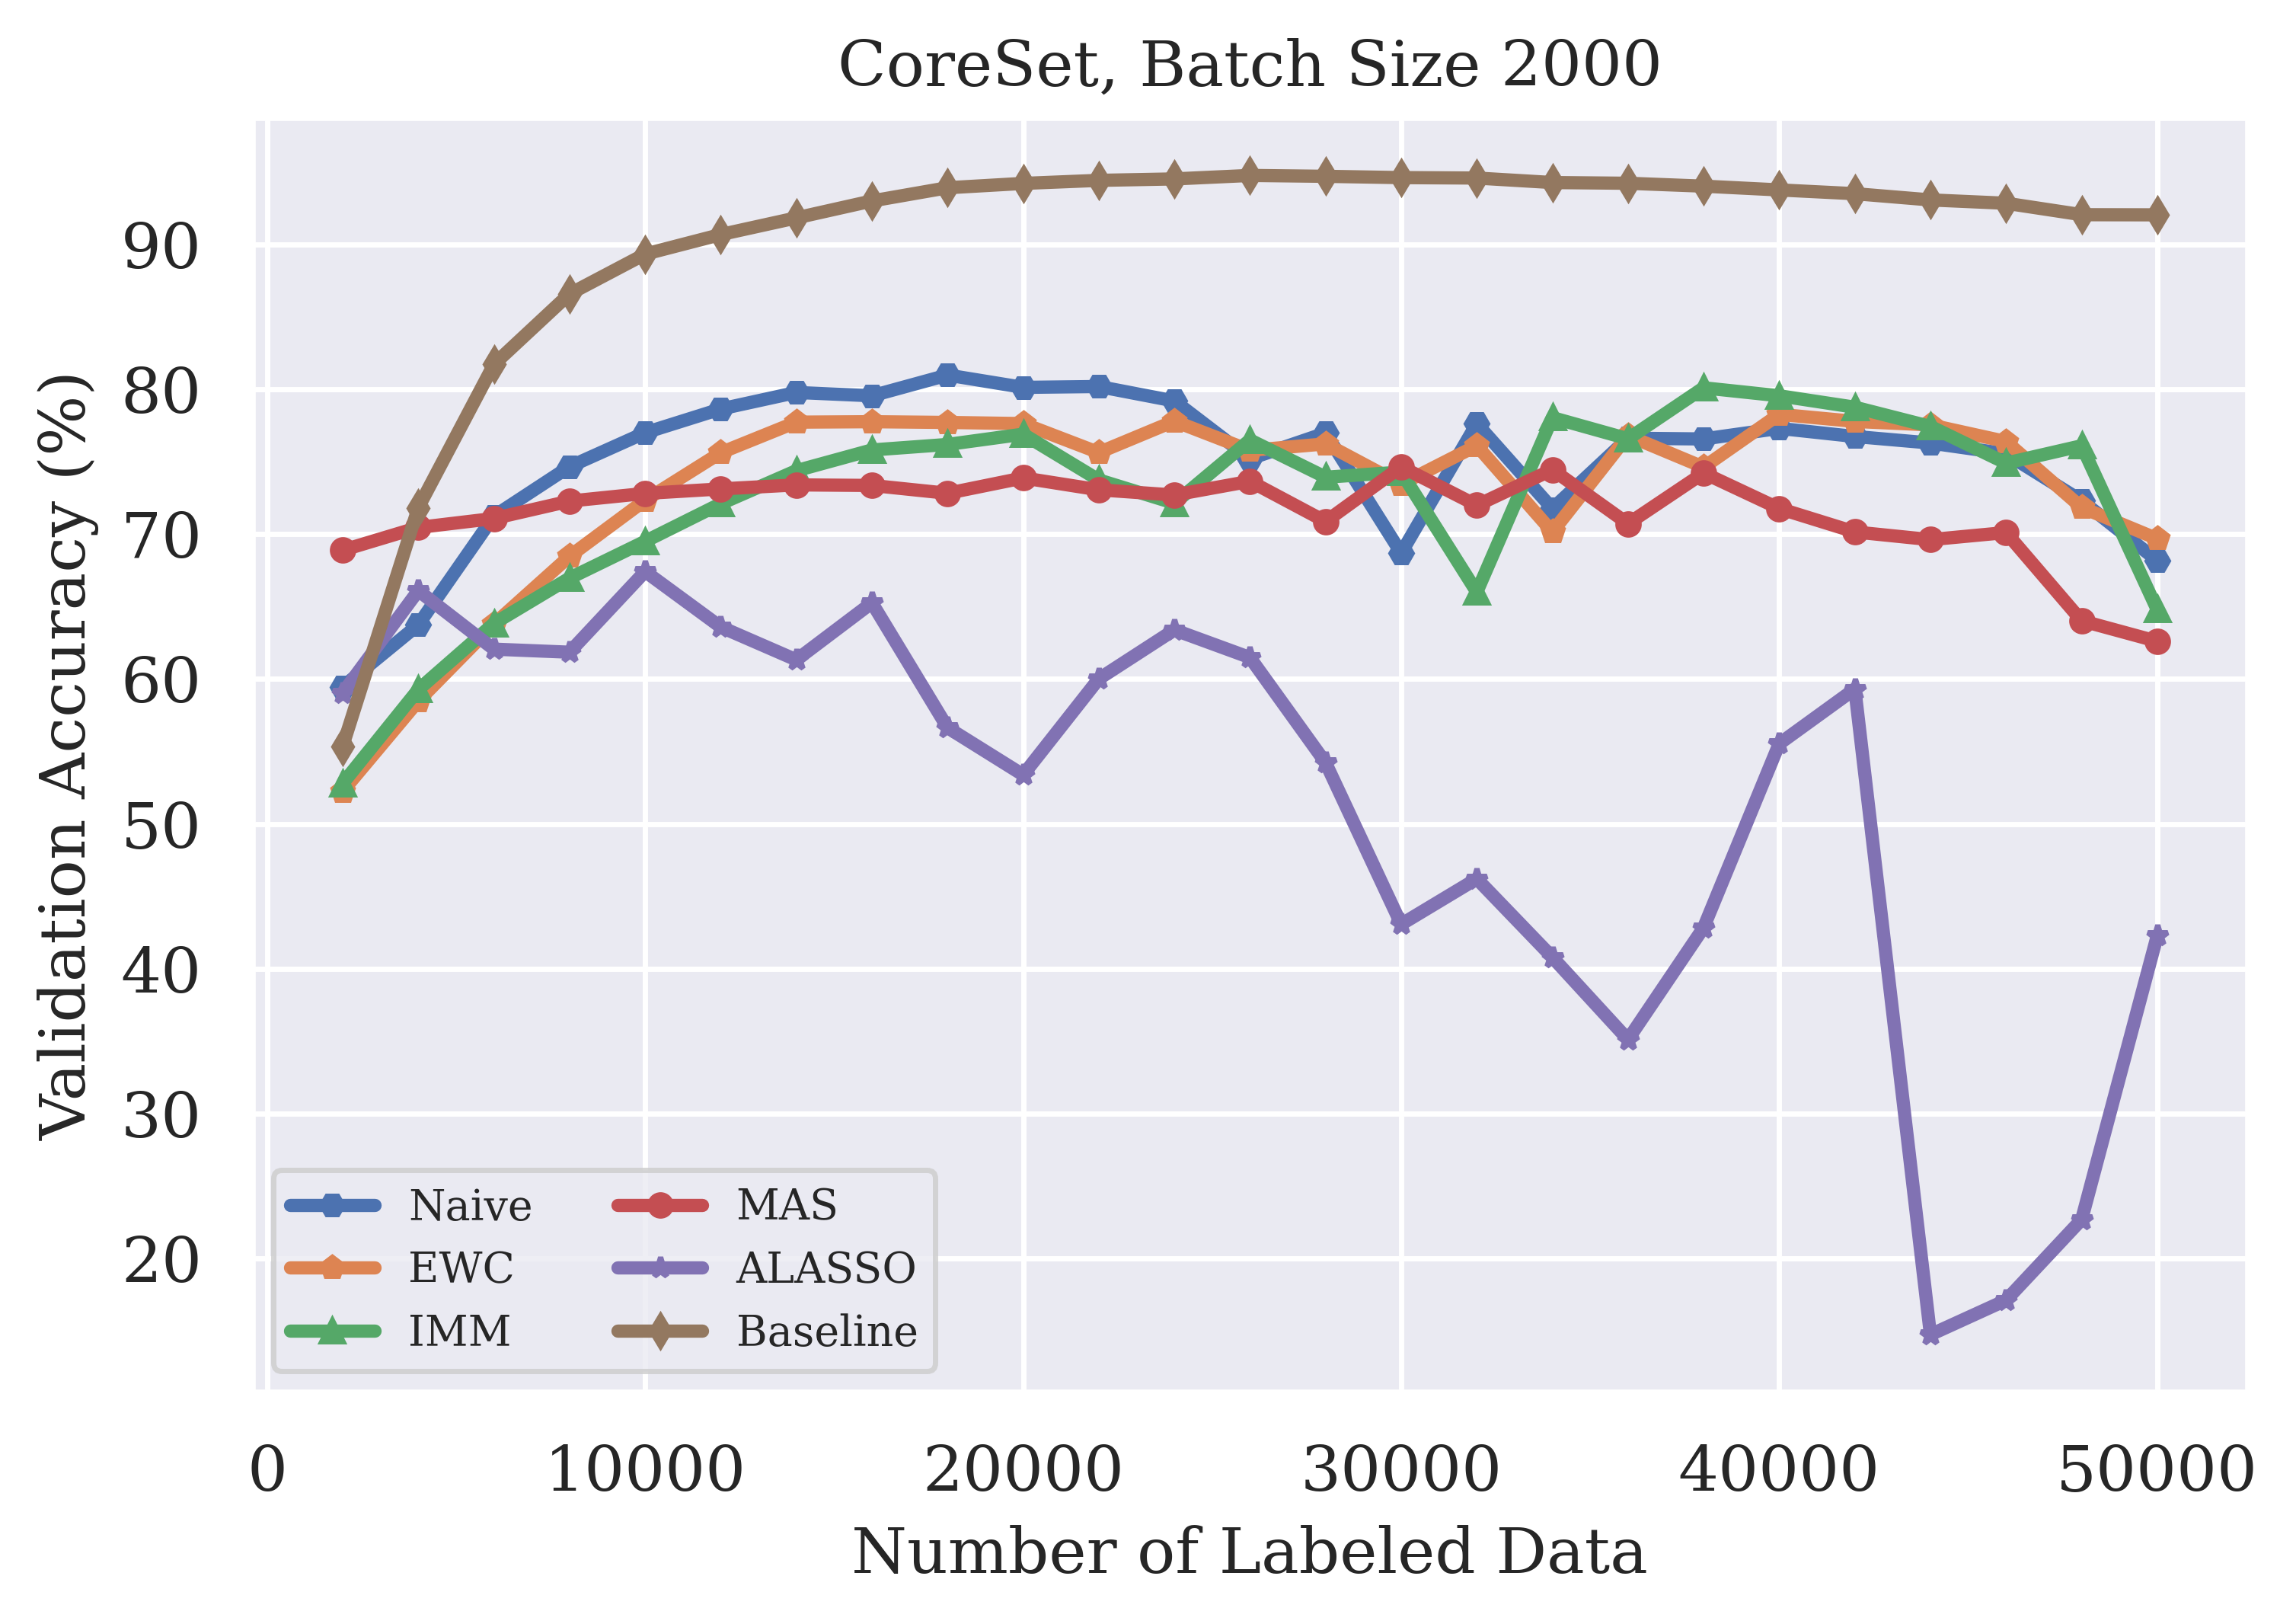
\includegraphics[width=0.32\linewidth]{images/results_CAL/coreset_2000b_acc.png} \hfill
    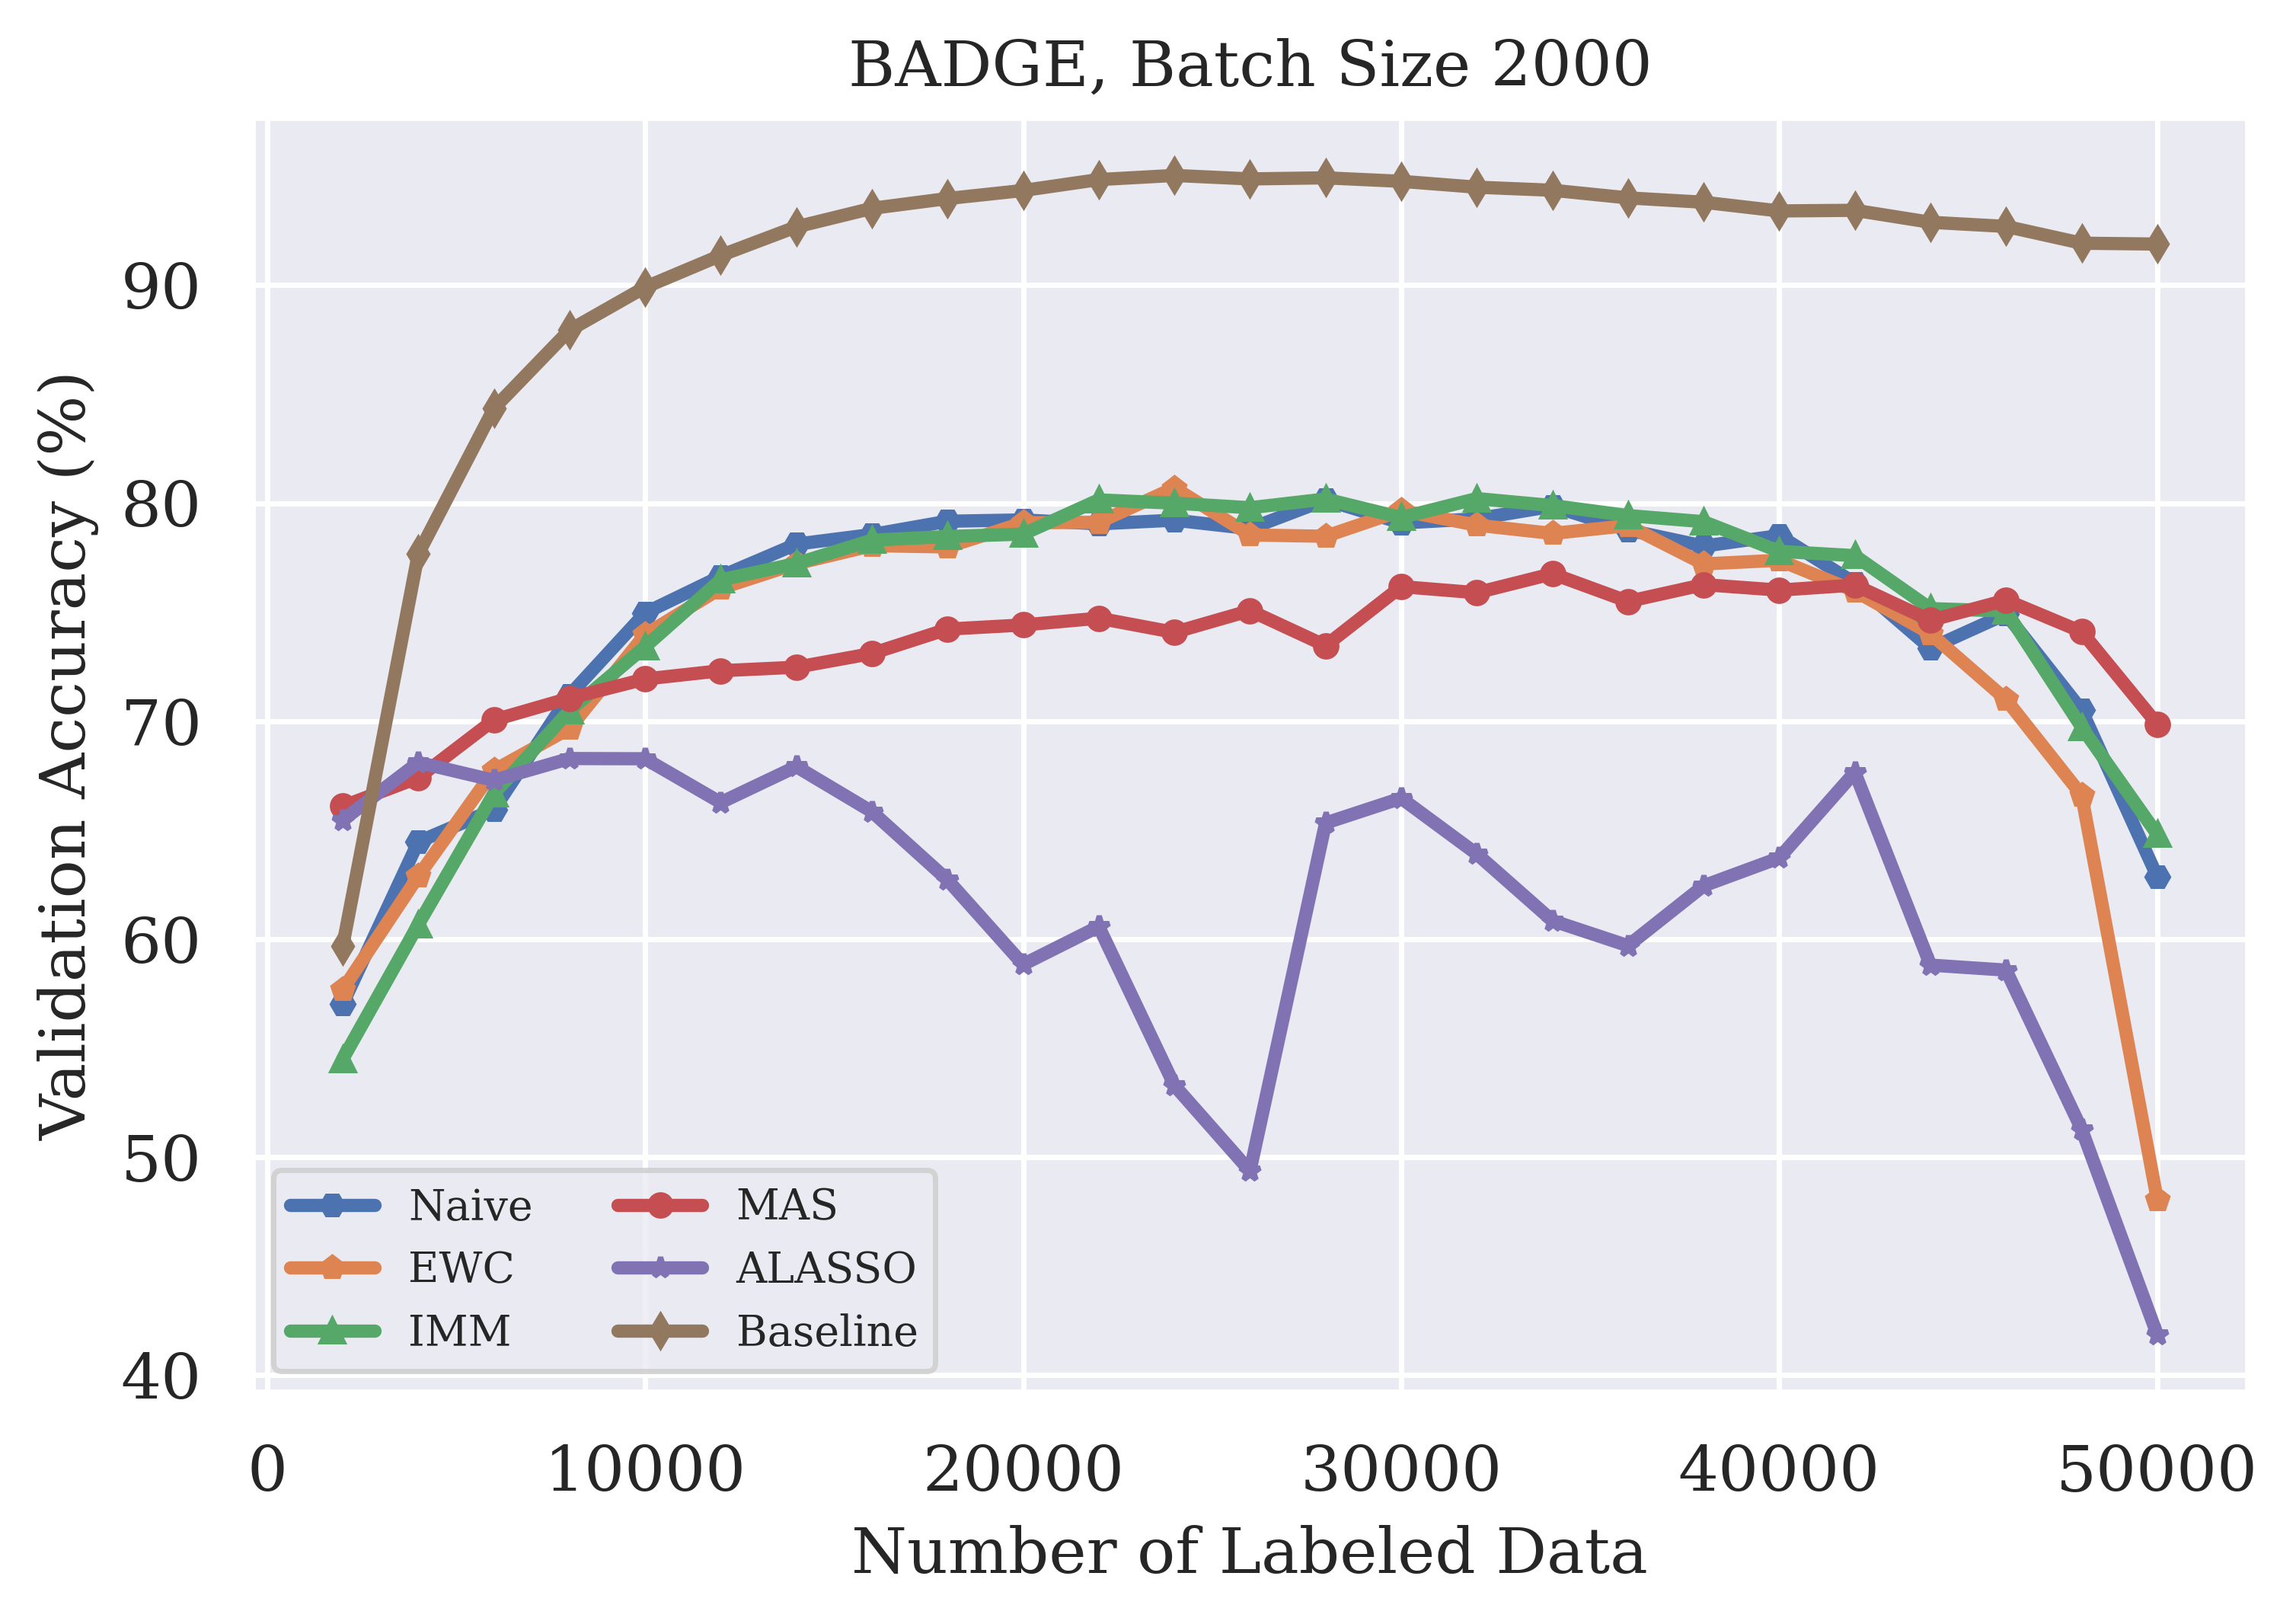
\includegraphics[width=0.32\linewidth]{images/results_CAL/badge_2000b_acc.png} \hfill
    \caption[Continual Active Learning with \gls{badge} with varying batch size]{Comparison of validation accuracy of Continual Learning and Active Learning strategies
    with batch size 2000.}
    \label{fig:Evaluation:Results:CAL:2000bAcc}
\end{figure}

% \begin{figure}[h]
%     \centering
%     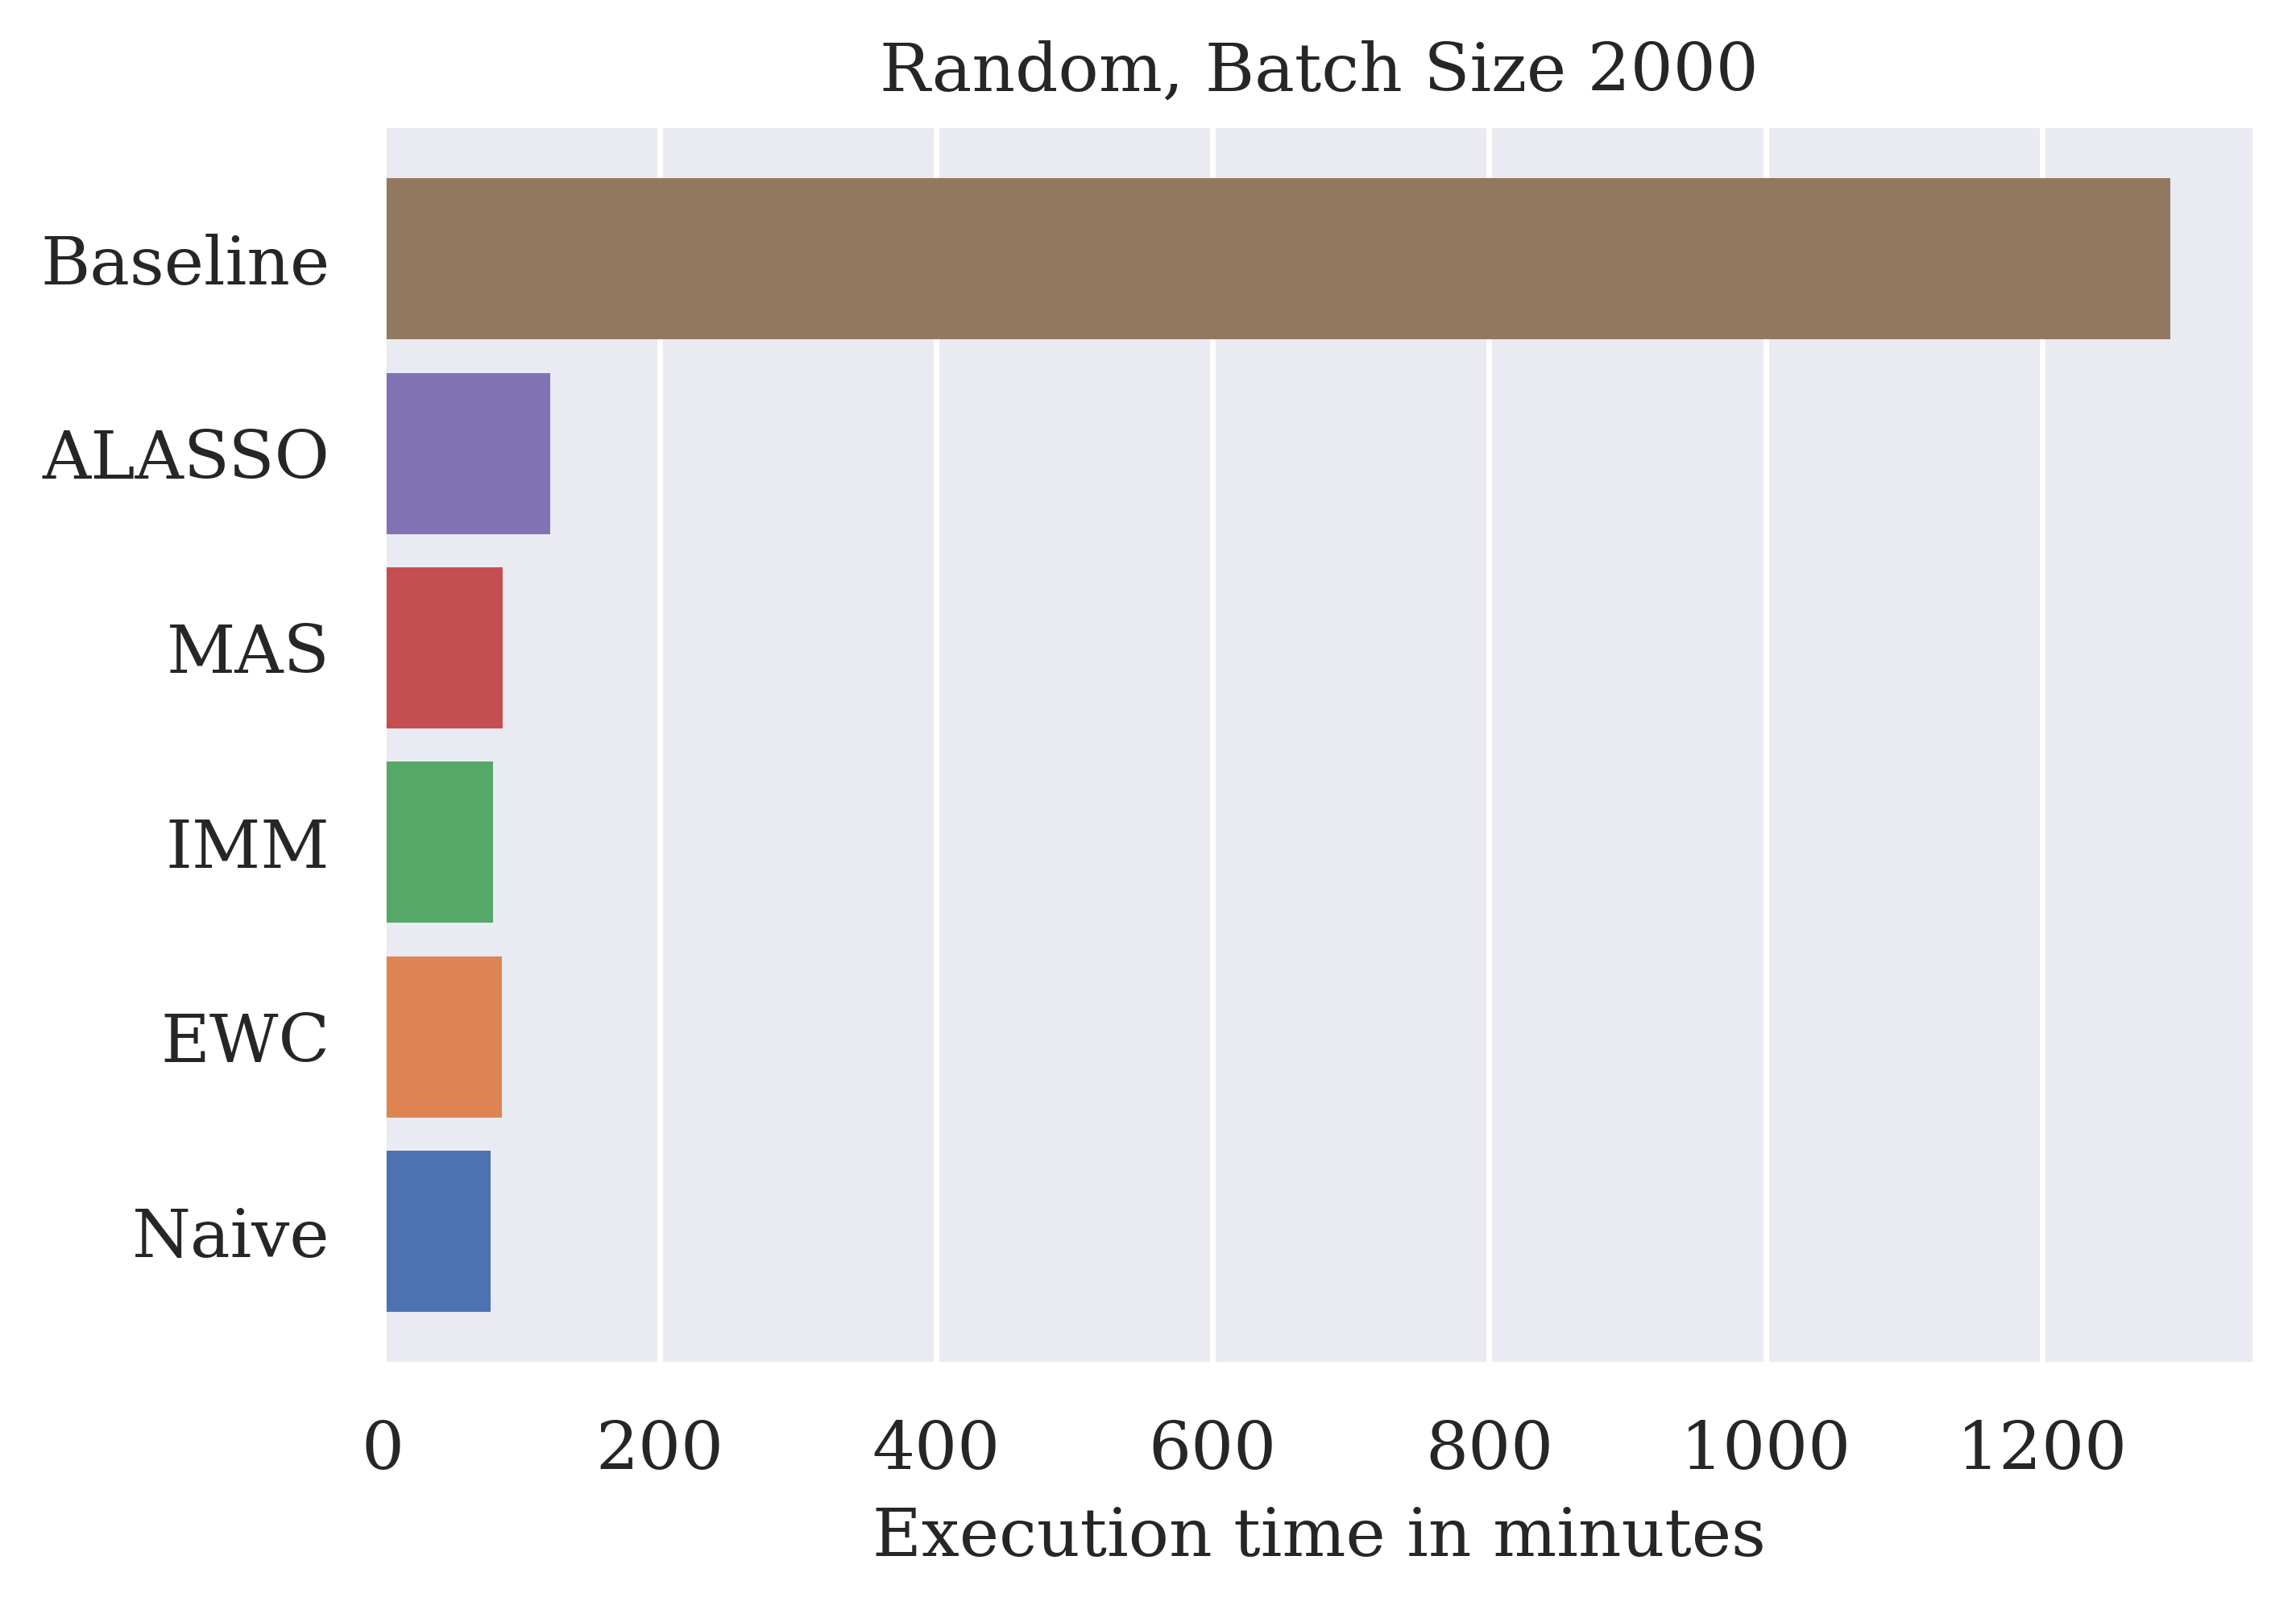
\includegraphics[width=0.32\linewidth]{images/results_CAL/random_2000b_time.png} \hfill
%     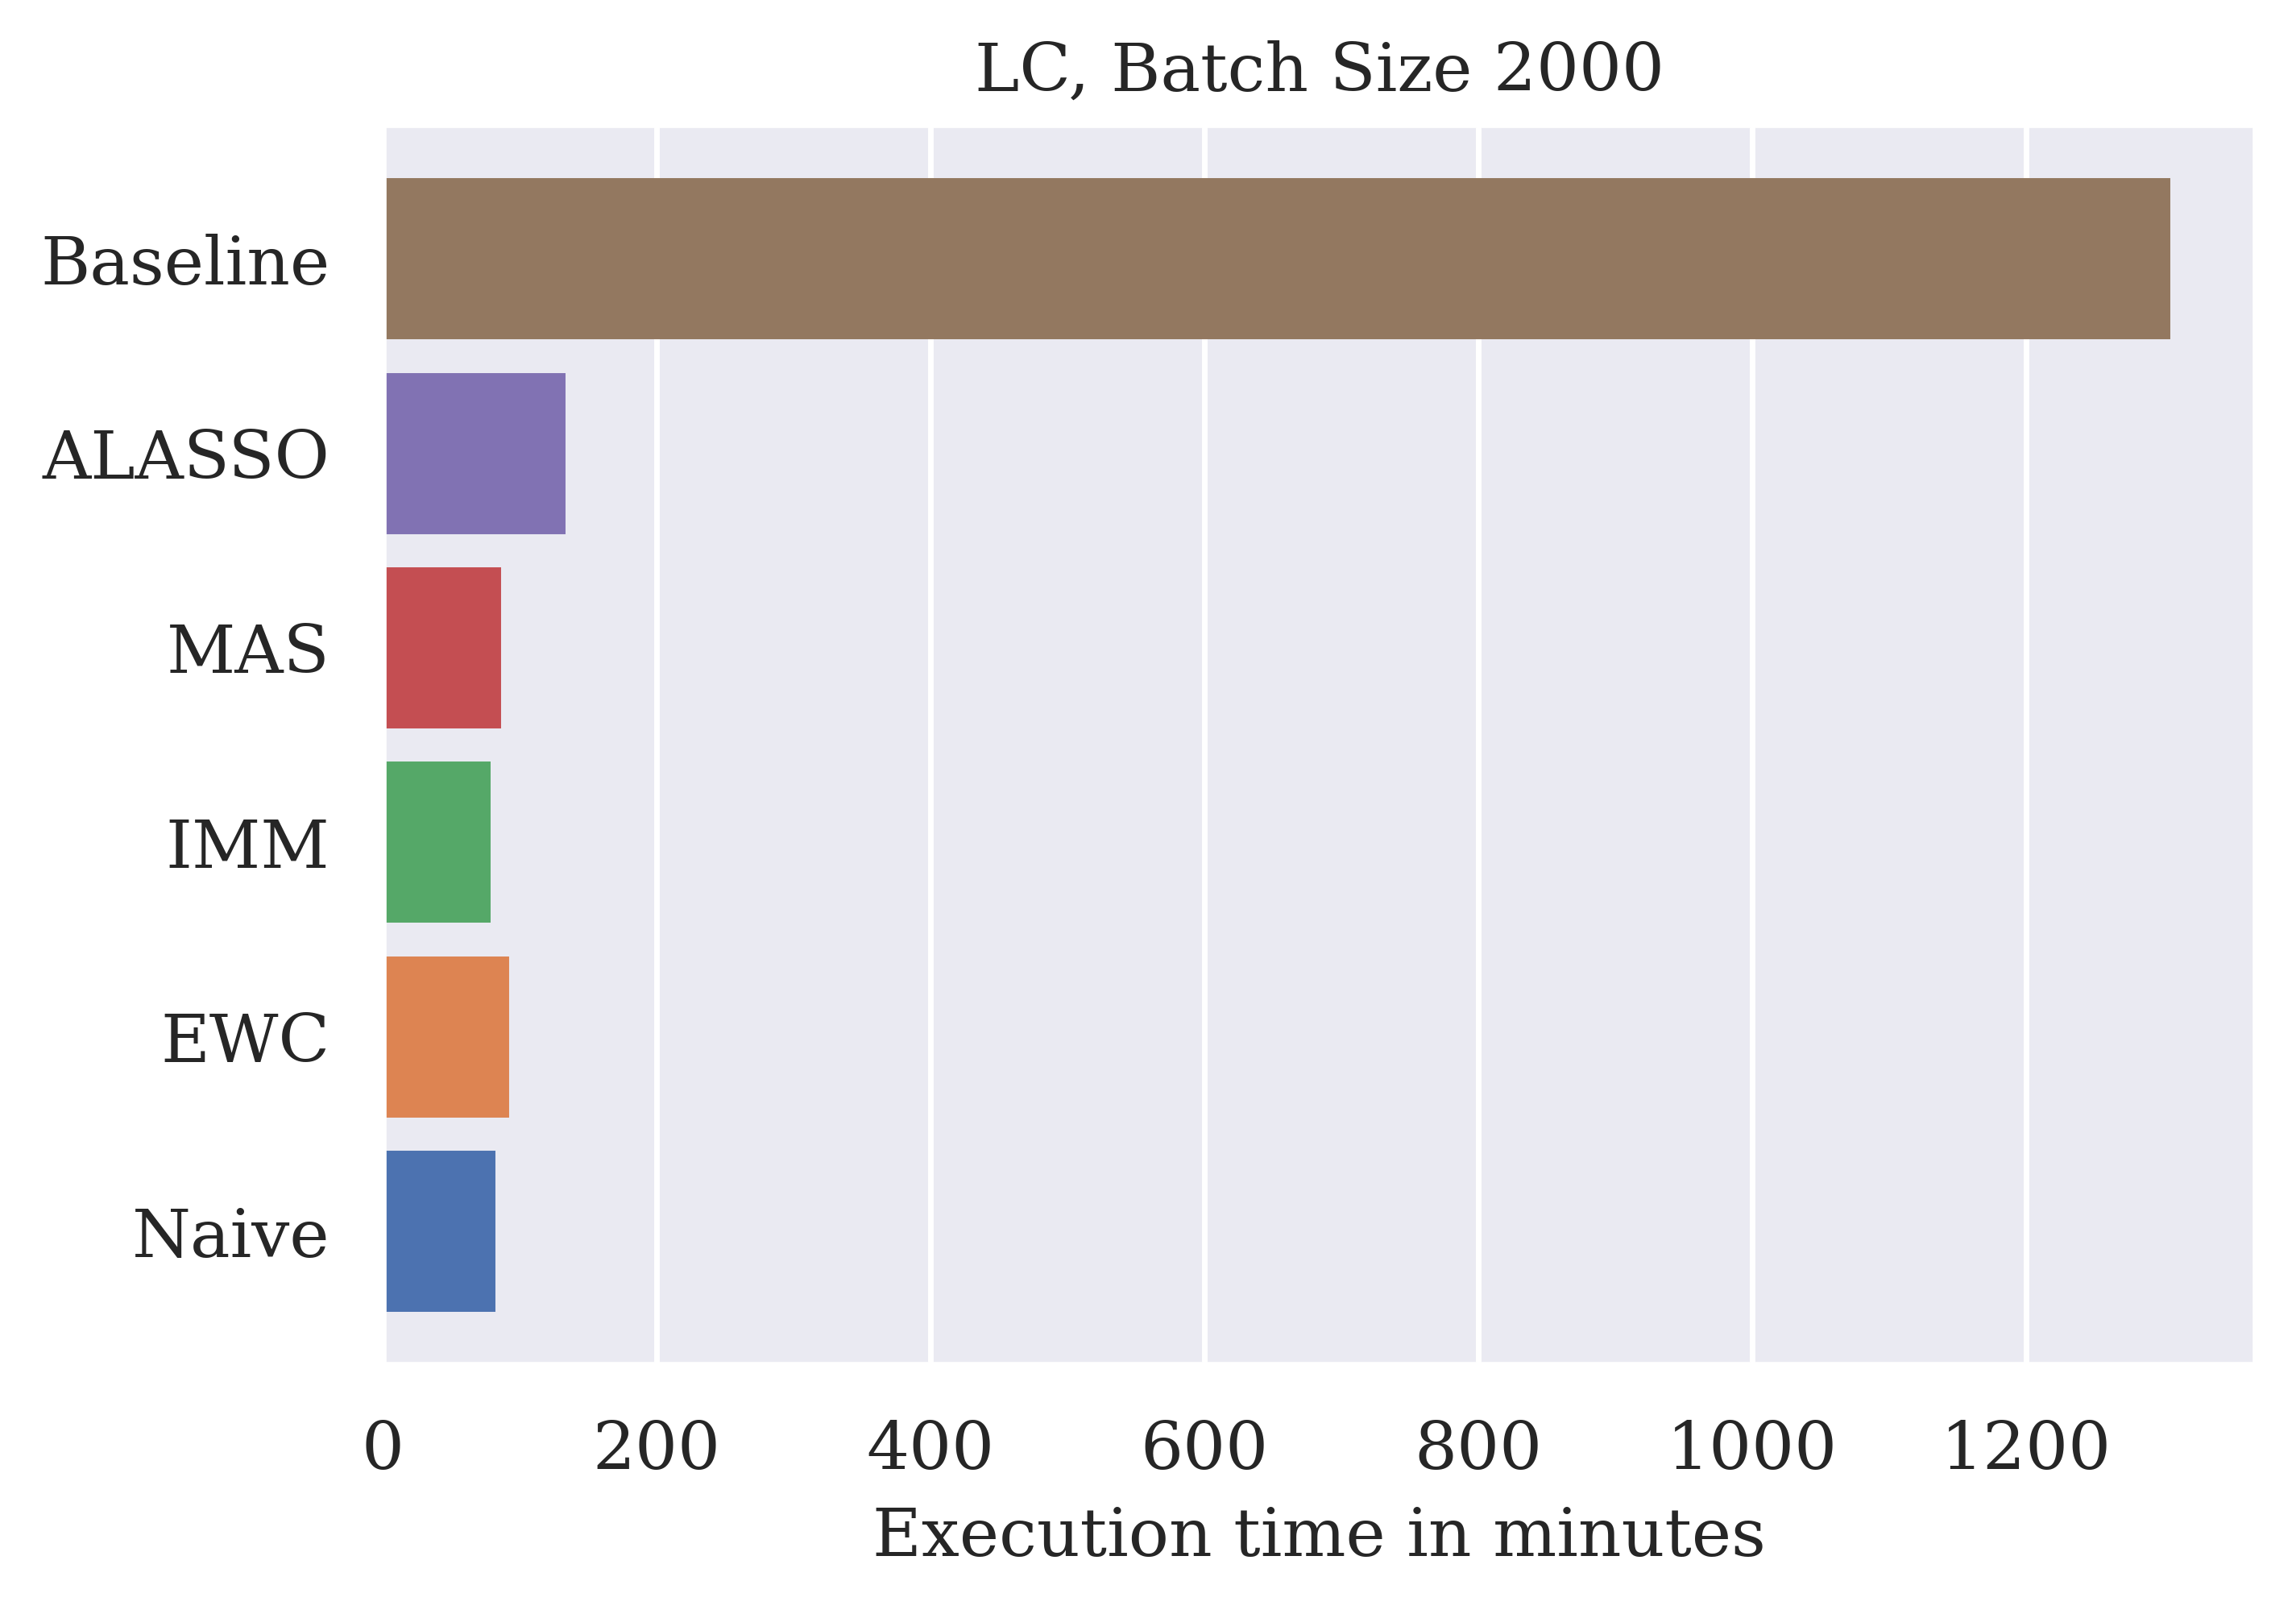
\includegraphics[width=0.32\linewidth]{images/results_CAL/lc_2000b_time.png} \hfill
%     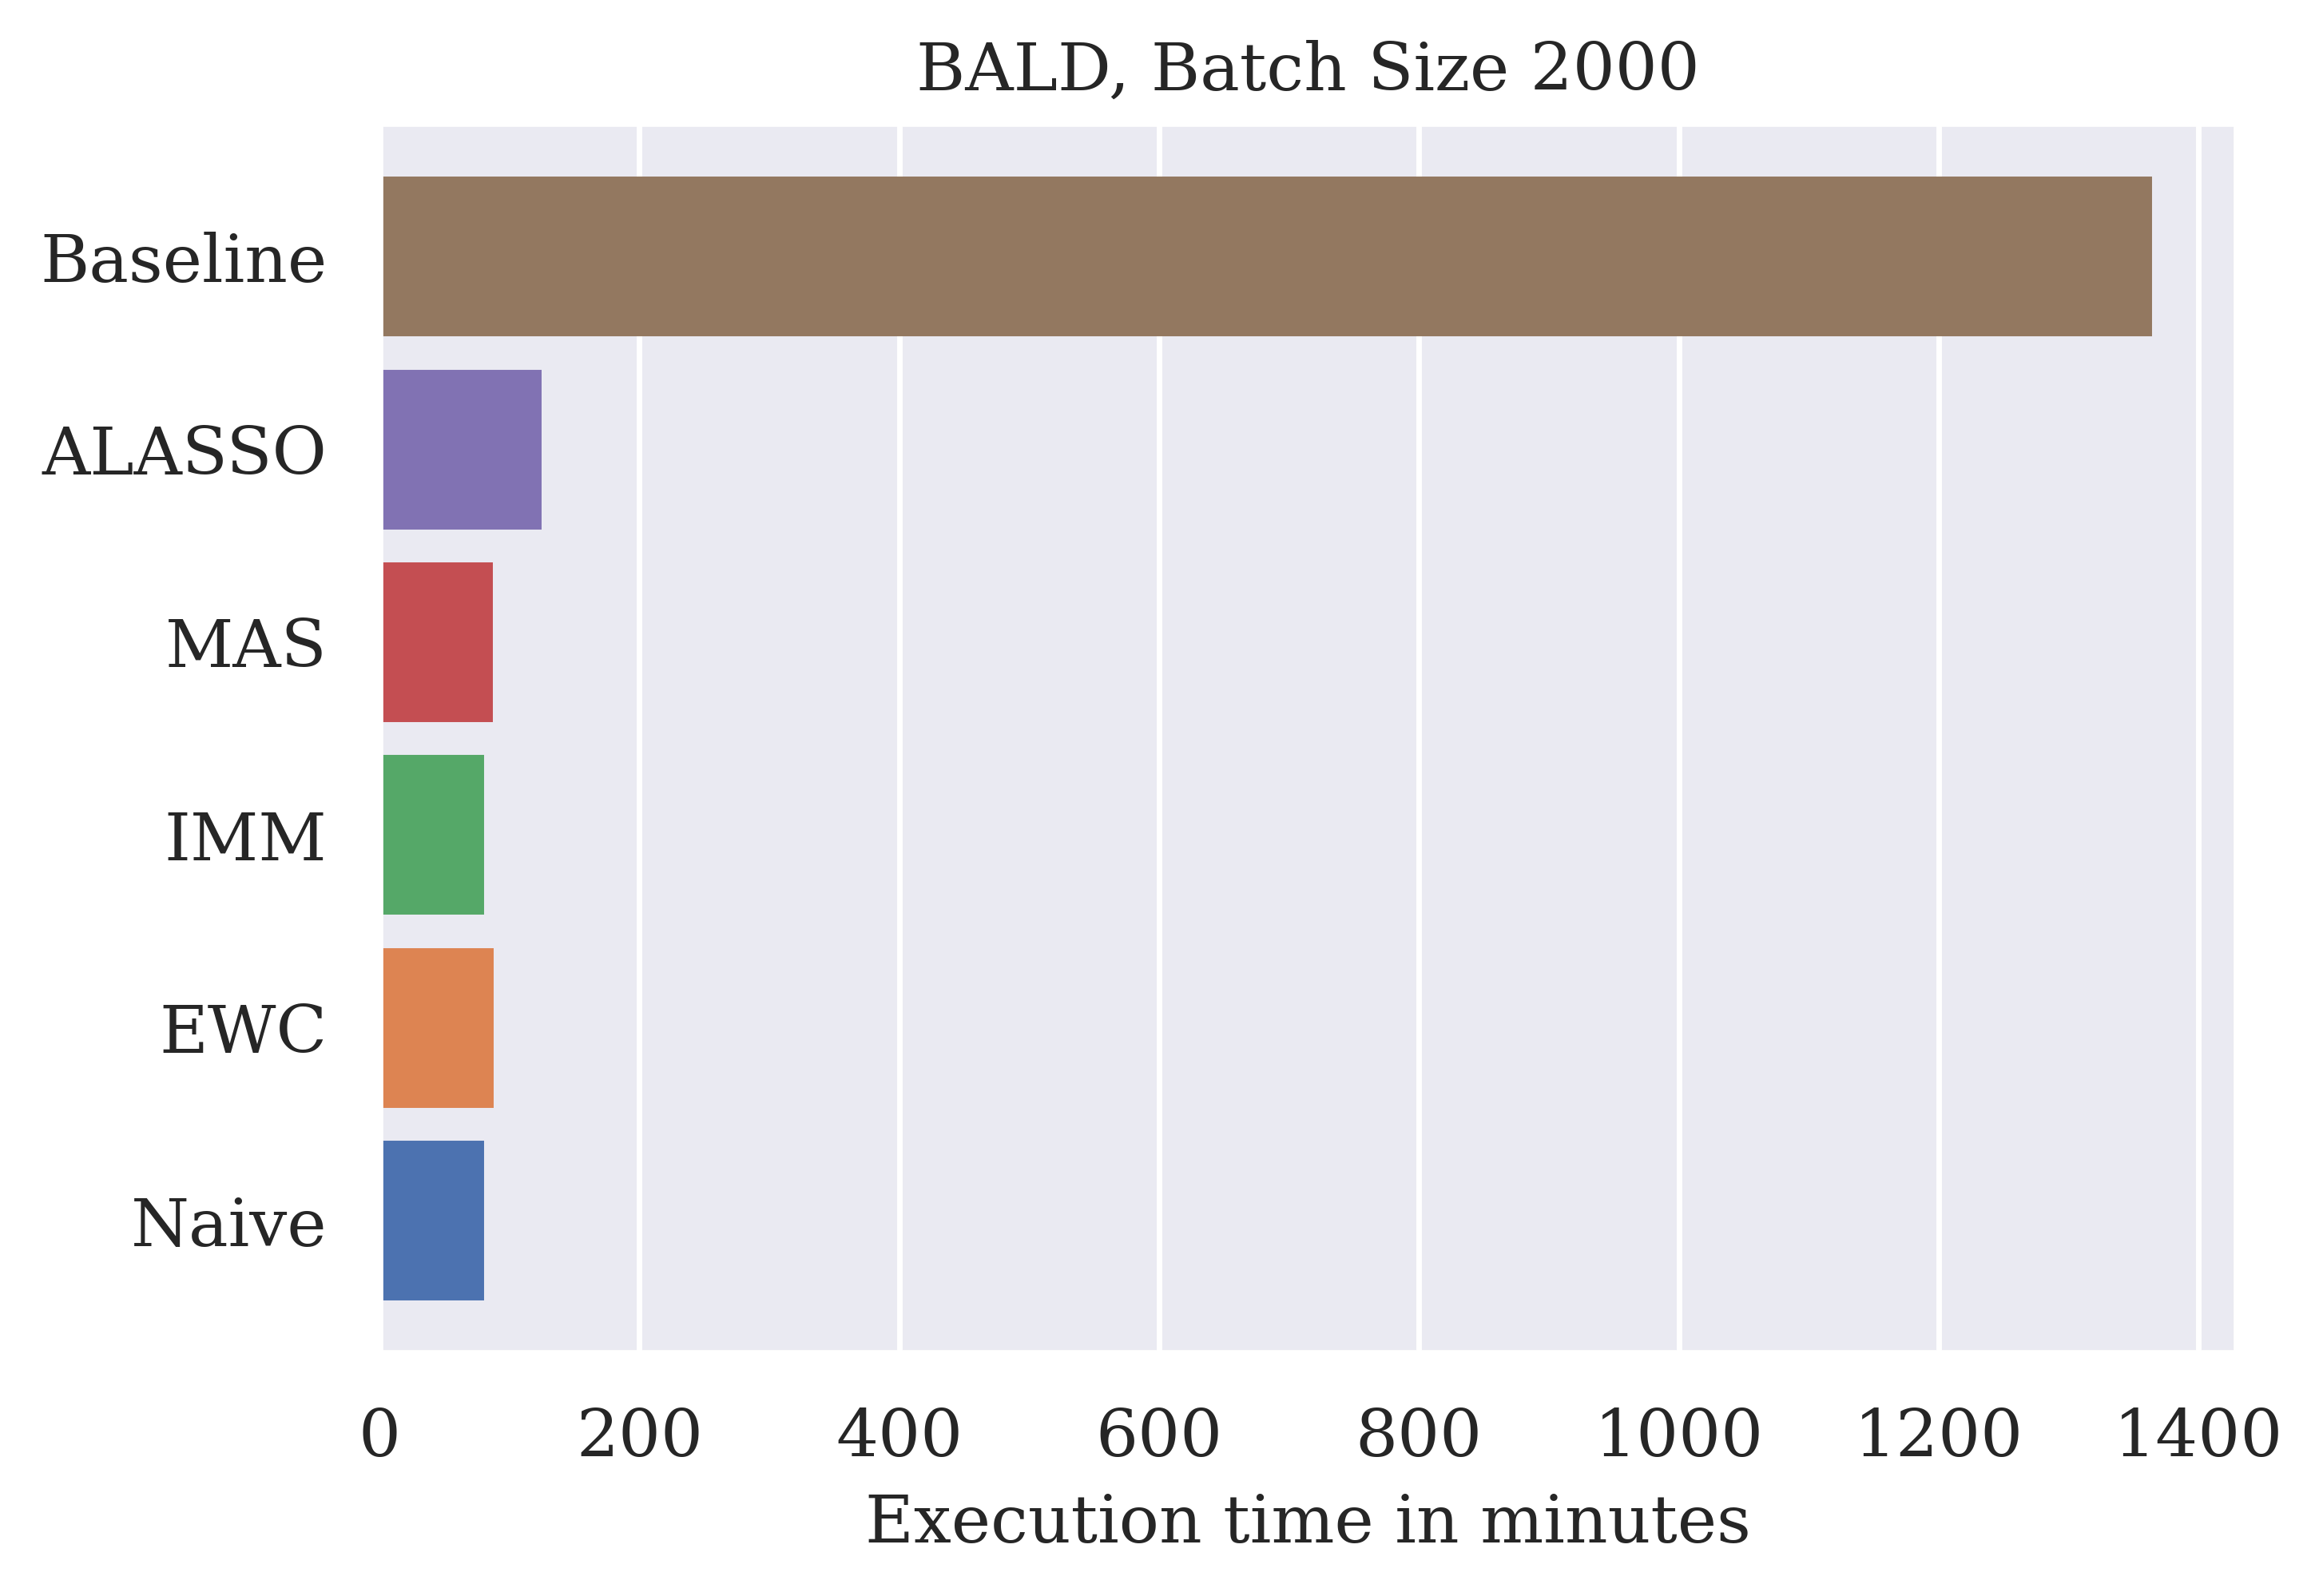
\includegraphics[width=0.32\linewidth]{images/results_CAL/bald_2000b_time.png}
%     \\[\smallskipamount]
%     \hfill 
%     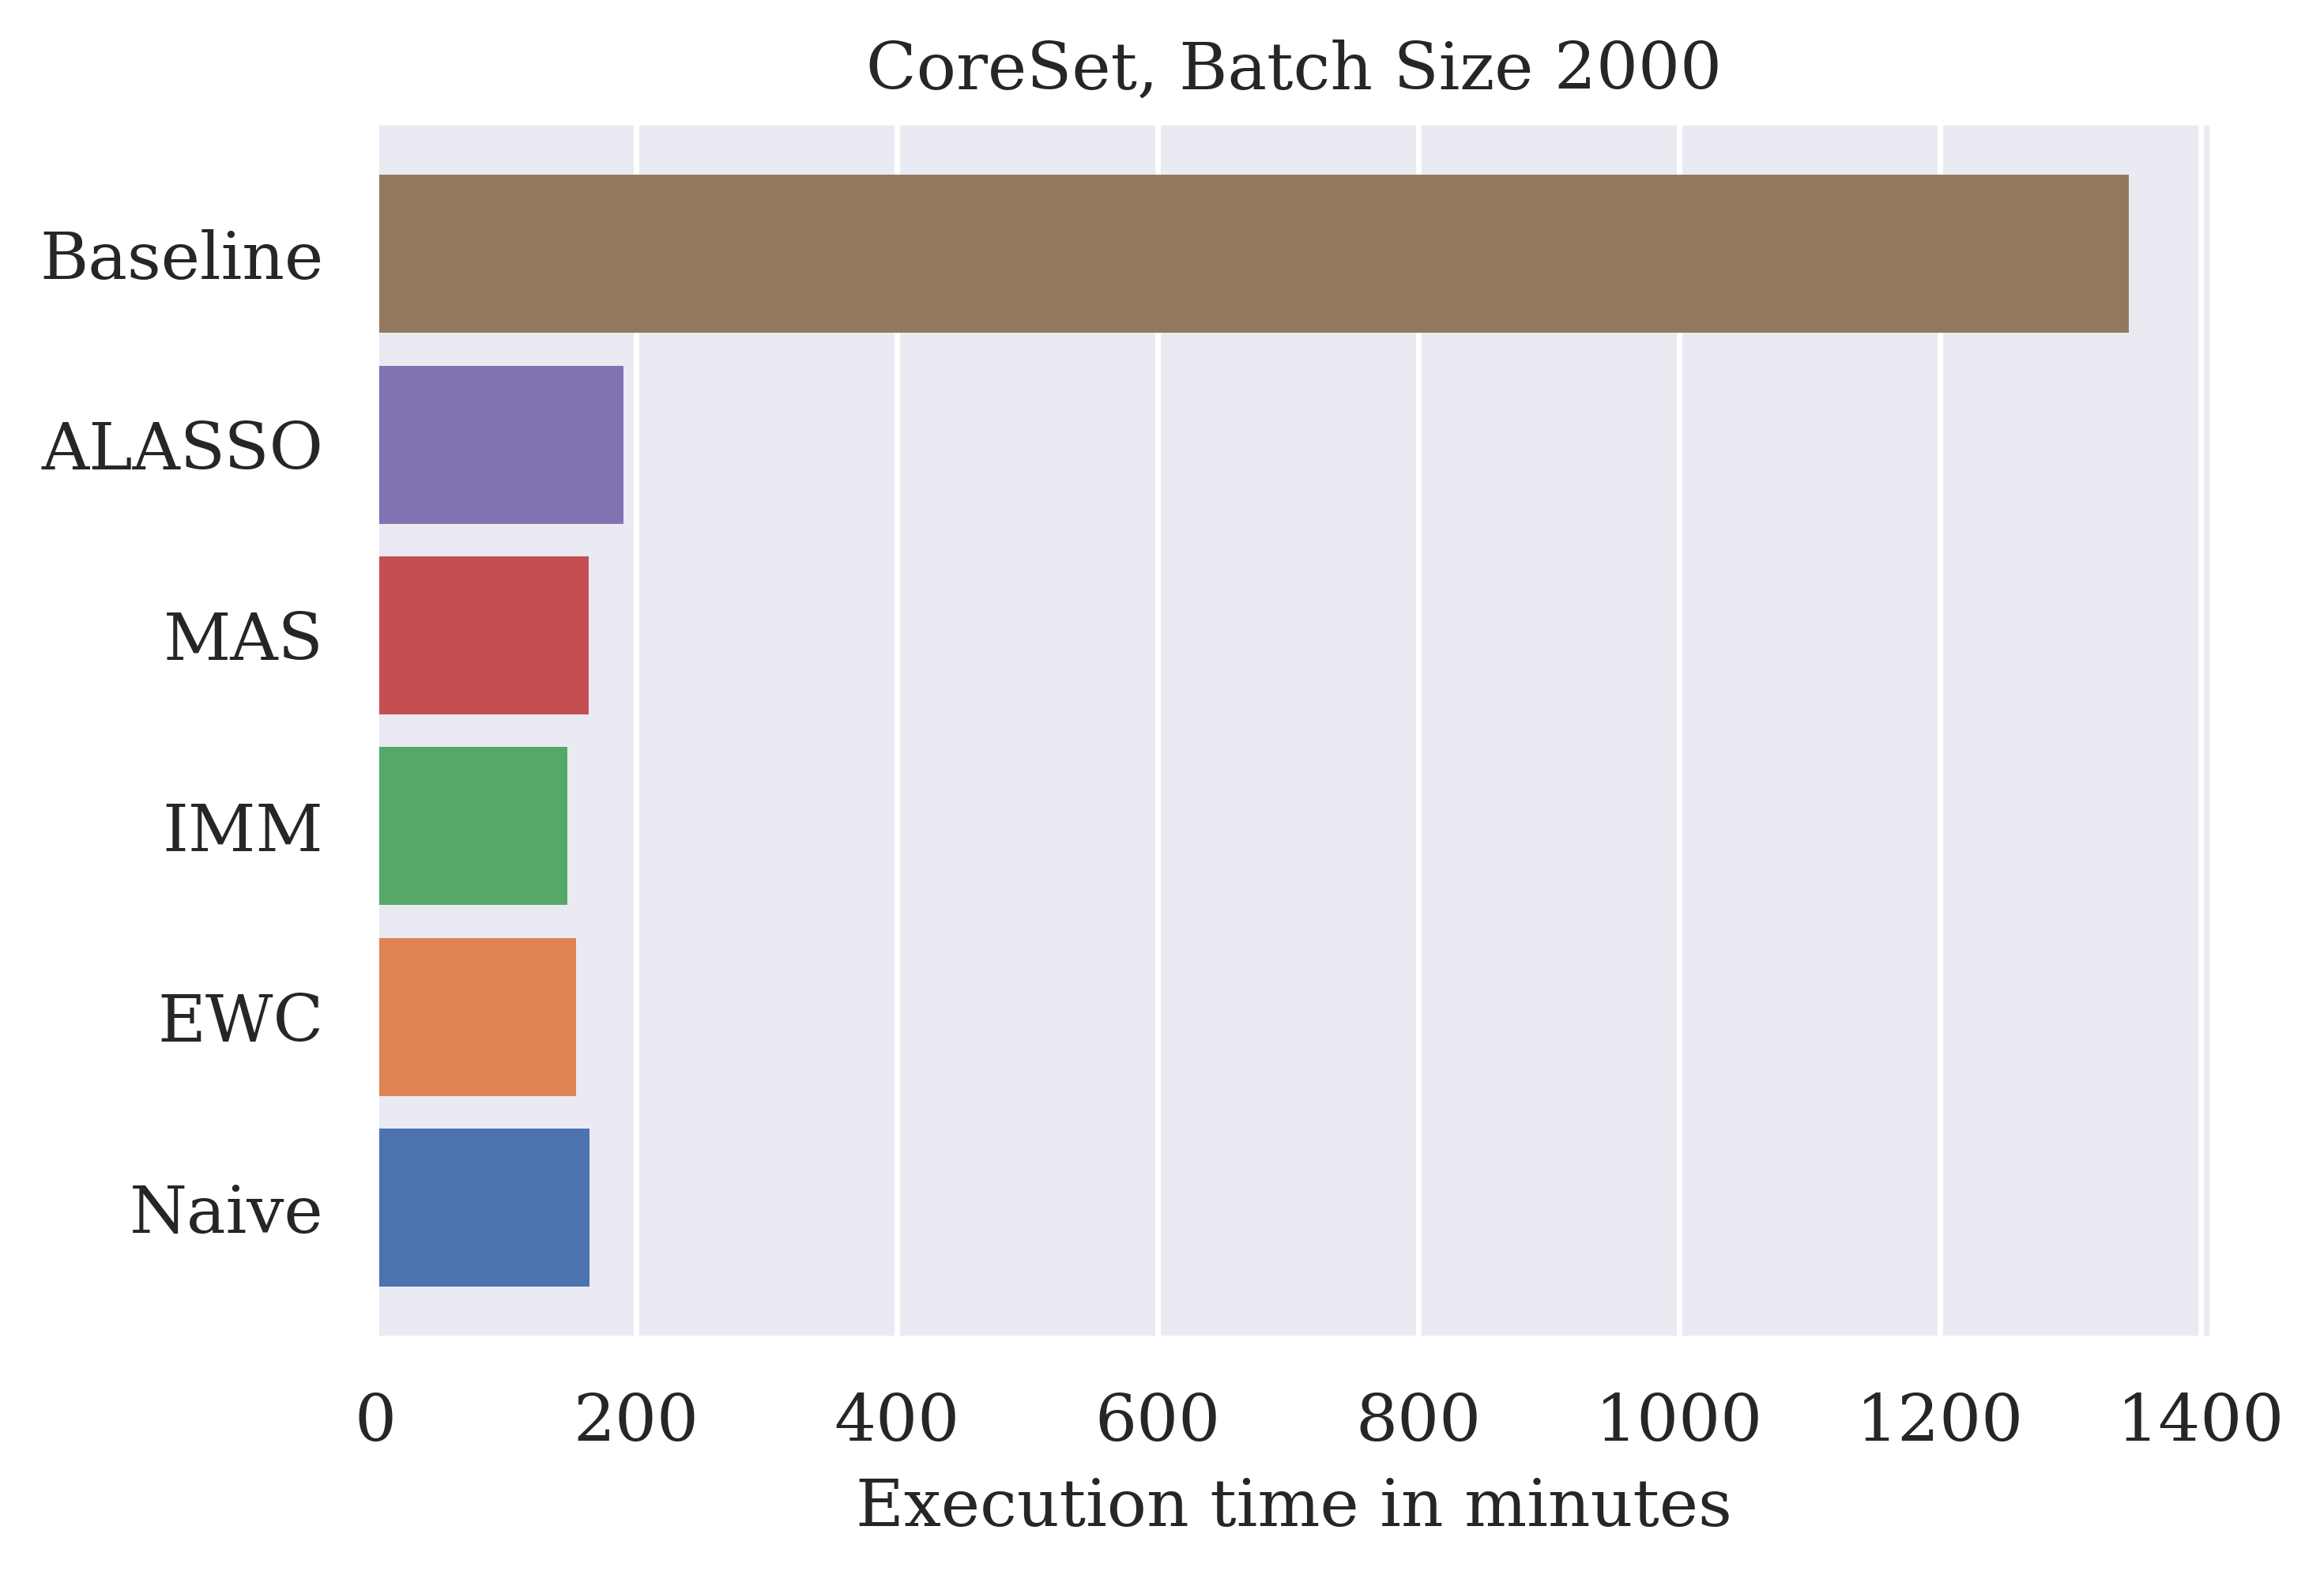
\includegraphics[width=0.32\linewidth]{images/results_CAL/coreset_2000b_time.png} \hfill
%     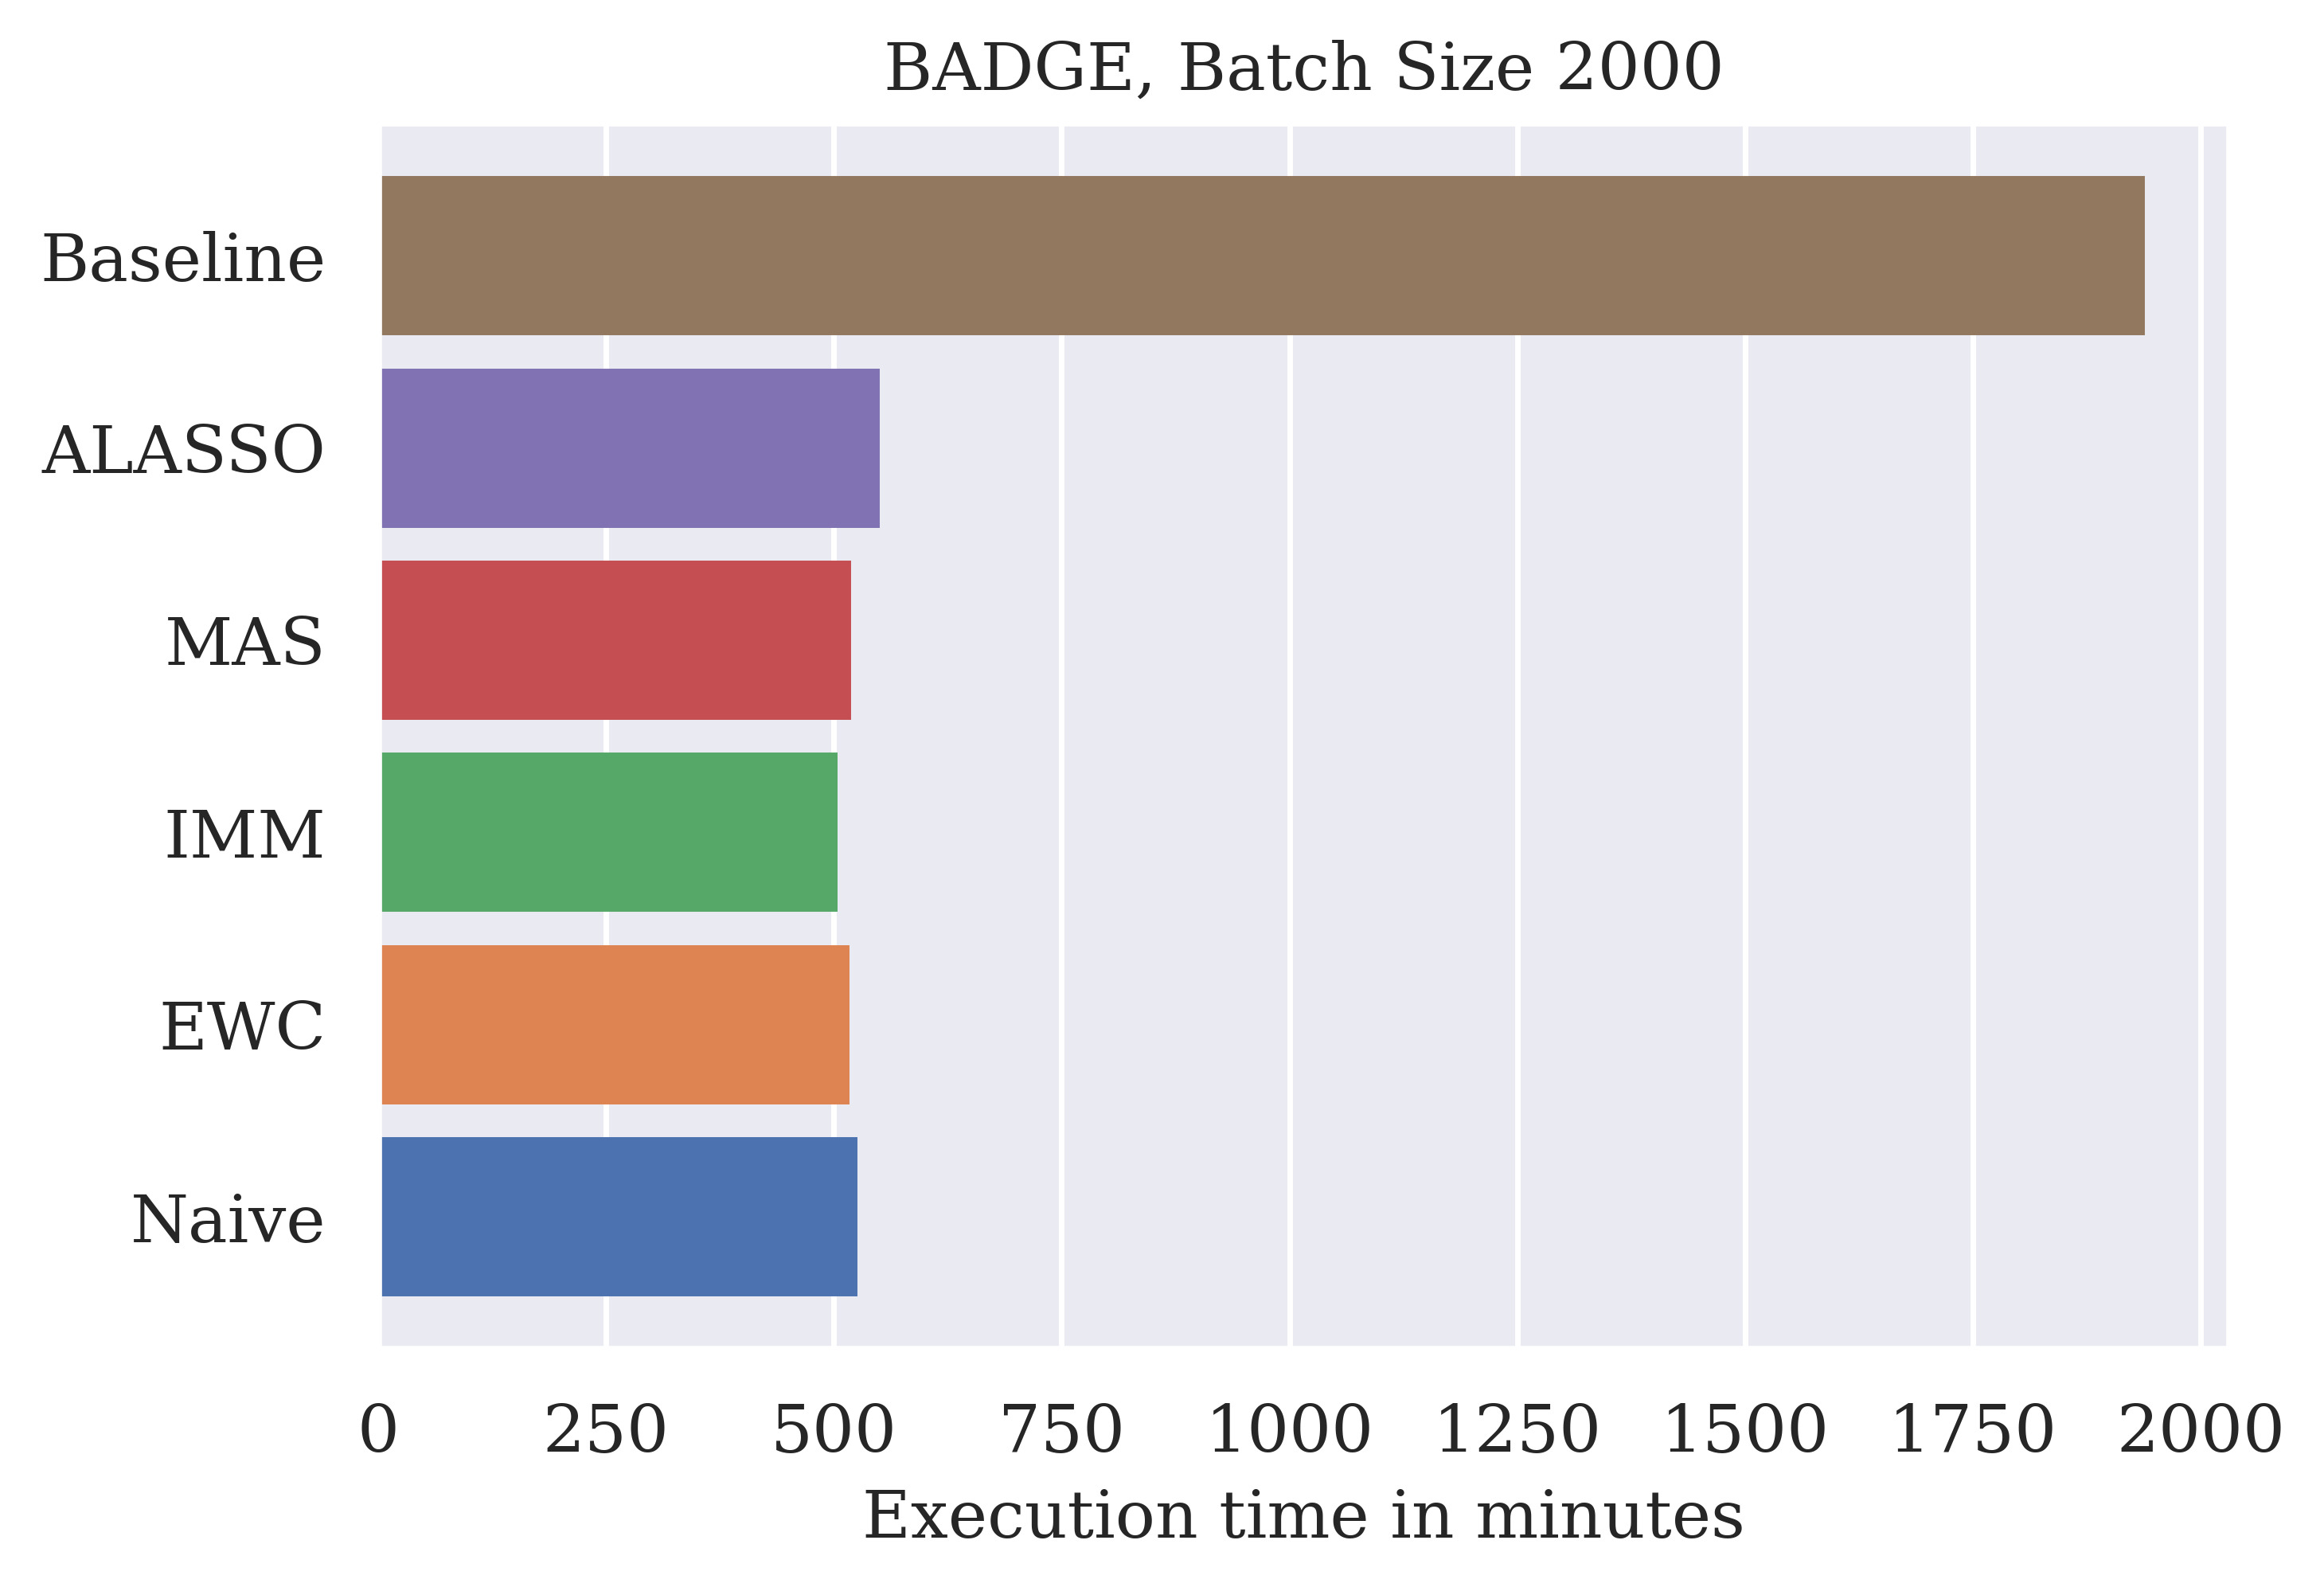
\includegraphics[width=0.32\linewidth]{images/results_CAL/badge_2000b_time.png} \hfill
%     \caption[Continual Active Learning with \gls{badge} with varying batch size]{Comparison of execution time of Continual Learning and Active Learning strategies
%     with batch size 2000.}
%     \label{fig:Evaluation:Results:CAL:2000bTime}
% \end{figure}

\begin{table}[h]
    \centering
    \begin{tabular}{c | c c c c c } 
         & Random & \gls{lc} & \gls{bald} & CoreSet & \gls{badge}\\ 
        \hline 
        Baseline & 1290 & 1303 & 1315 & 1342 & 1935 \\
        \hline
        Naive & 76 & 80 & 78 & 162 & 523 \\
        \gls{ewc} & 83 & 90 & 86 & 152 & 513\\
        \gls{imm} & 77 & 76 & 78 & 145 & 500\\
        \gls{mas} & 84 & 84 & 85 & 161 & 515\\
        \gls{alasso} & 119 & 131 & 122 & 188 & 547\\
    \end{tabular}
    \caption{Comparison of execution time of regularization-based continual learning strategies
    with batch size 2000.}
    \label{fig:Evaluation:Results:CAL:2000bTimeTable}
\end{table}

\section{Model Stealing}
\label{sec:Appendix:MS}

\subsection{Evaluation of ActiveThief}
\label{sec:Appendix:MS:ActiveThief}
Because we build our Continual Active Learning approach upon the ActiveThief framework, we believe that it is important to rigorously evaluate it before we apply Continual Active Learning to it. In the ActiveThief paper \cite{pal2020activethief}, Pal et al. evaluate Active Learning
for Model Stealing for Computer Vision and Natural Language Processing tasks. Since this thesis focuses on Computer Vision tasks, we only investigate the part of the ActiveThief framework that deals with Computer Vision tasks. For the ActiveThief framework, Pal et al. introduce a
proprietary thief dataset, which we dubbed SmallImagenet, and three different target model architectures which we call ActiveThiefConv2, ActiveThiefConv3 and ActiveThiefConv4. In the following we will evaluate the influence of the thief dataset and the target model architecture on
the success of the Model Stealing attack. \par
We start off by computing the validation accuracies of the ActiveThiefConv Model family which both the ActiveThief framework and ours uses as target and substitute models. While these figures have not been given by the authors of ActiveThief in their paper, we believe that they are
important to understand the performance of the ActiveThief framework and of our Continual Active Learning approach. Each model of the ActiveThiefConv family is trained on MNIST and CIFAR-10. Additionally, we train ActiveThiefConv3 on CIFAR-100, because we will conduct experiments
with CIFAR-100 in section \ref{sec:Evaluation:Results:MS:CAL}. We omit the results for ActiveThiefConv2 and ActiveThiefConv4 on CIFAR-100 because they are not relevant to this thesis. The results can be found in table \ref{fig:TargetModelAccuracies}. The results show that the
most complex model ActiveThiefConv4 achieves the highest validation accuracy on both MNIST and CIFAR-10. While the validation accuracy for MNIST is very high for all models, there is a difference in validation accuracy of almost 20 percentage points between ActiveThiefConv2 and
ActiveThiefConv4 on CIFAR-10. This shows that the complexity of the target model architecture has a significant influence on the validation accuracy. \par

\begin{table}[h]
    \centering
    \begin{tabular}{|c|| c | c | c|} 
        \hline
        & ActiveThiefConv2 & ActiveThiefConv3 & ActiveThiefConv4 \\ 
        \hline 
        MNIST & 98.42 & 98.91 & 99.01 \\
        \hline
        CIFAR-10 & 66.61 & 80.67 & 84.47 \\
        \hline
        CIFAR-100 & - & 42.90 & - \\
        \hline
    \end{tabular}
    \caption[Validation accuracies of our target model architectures]{Validation accuracies (in \%) of our target model architectures on MNIST, CIFAR-10 and CIFAR-100. 
    We omit the results for ActiveThiefConv2 and ActiveThiefConv4 on CIFAR-100 because they are not used in the experiments.}
    \label{fig:TargetModelAccuracies}
\end{table}

Next, we evaluate the influence of the target model architecture and substitute model architecture on the success of the Model Stealing attack. We use the ActiveThiefConv Model family as target and substitute models and perform one model stealing attack for each combination of
target and substitute model. We use the Active Learning strategy CoreSet with a batch size of 1000 and a total budget of 20000 to perform the attacks. The results can be seen in table \ref{fig:ModelStealingNNArchitecturesCIFAR}. The numbers reported in the table represent the 
agreement between the target and substitute model on the validation set of the CIFAR-10 dataset at the end of each experiment. Overall, we observe that the agreement between the target and substitute model is highest when we use a target model of low complexity (i.e. ActiveThiefCon2)
and a substitute model of moderate to high complexity (i.e. ActiveThiefConv3 and ActiveThiefConv4). This is in line with the results of the ActiveThief paper \cite{pal2020activethief}, however we report the accuracy after a budget of 20000, whereas Pal et al. presumably report the
accuracy after training on the full thief dataset. To study the behavior of model stealing attacks using different model architectures further, we conduct the same experiment using MNIST as the target model dataset. The results of this experiment can be found in table 
\ref{fig:ModelStealingNNArchitecturesMNIST}. The results of this experiment are similar to the results of the experiment on CIFAR-10, however it is evident that the discrepancies between the target and substitute model combinations are larger. \par

\begin{figure}[!htb]
    \centering
    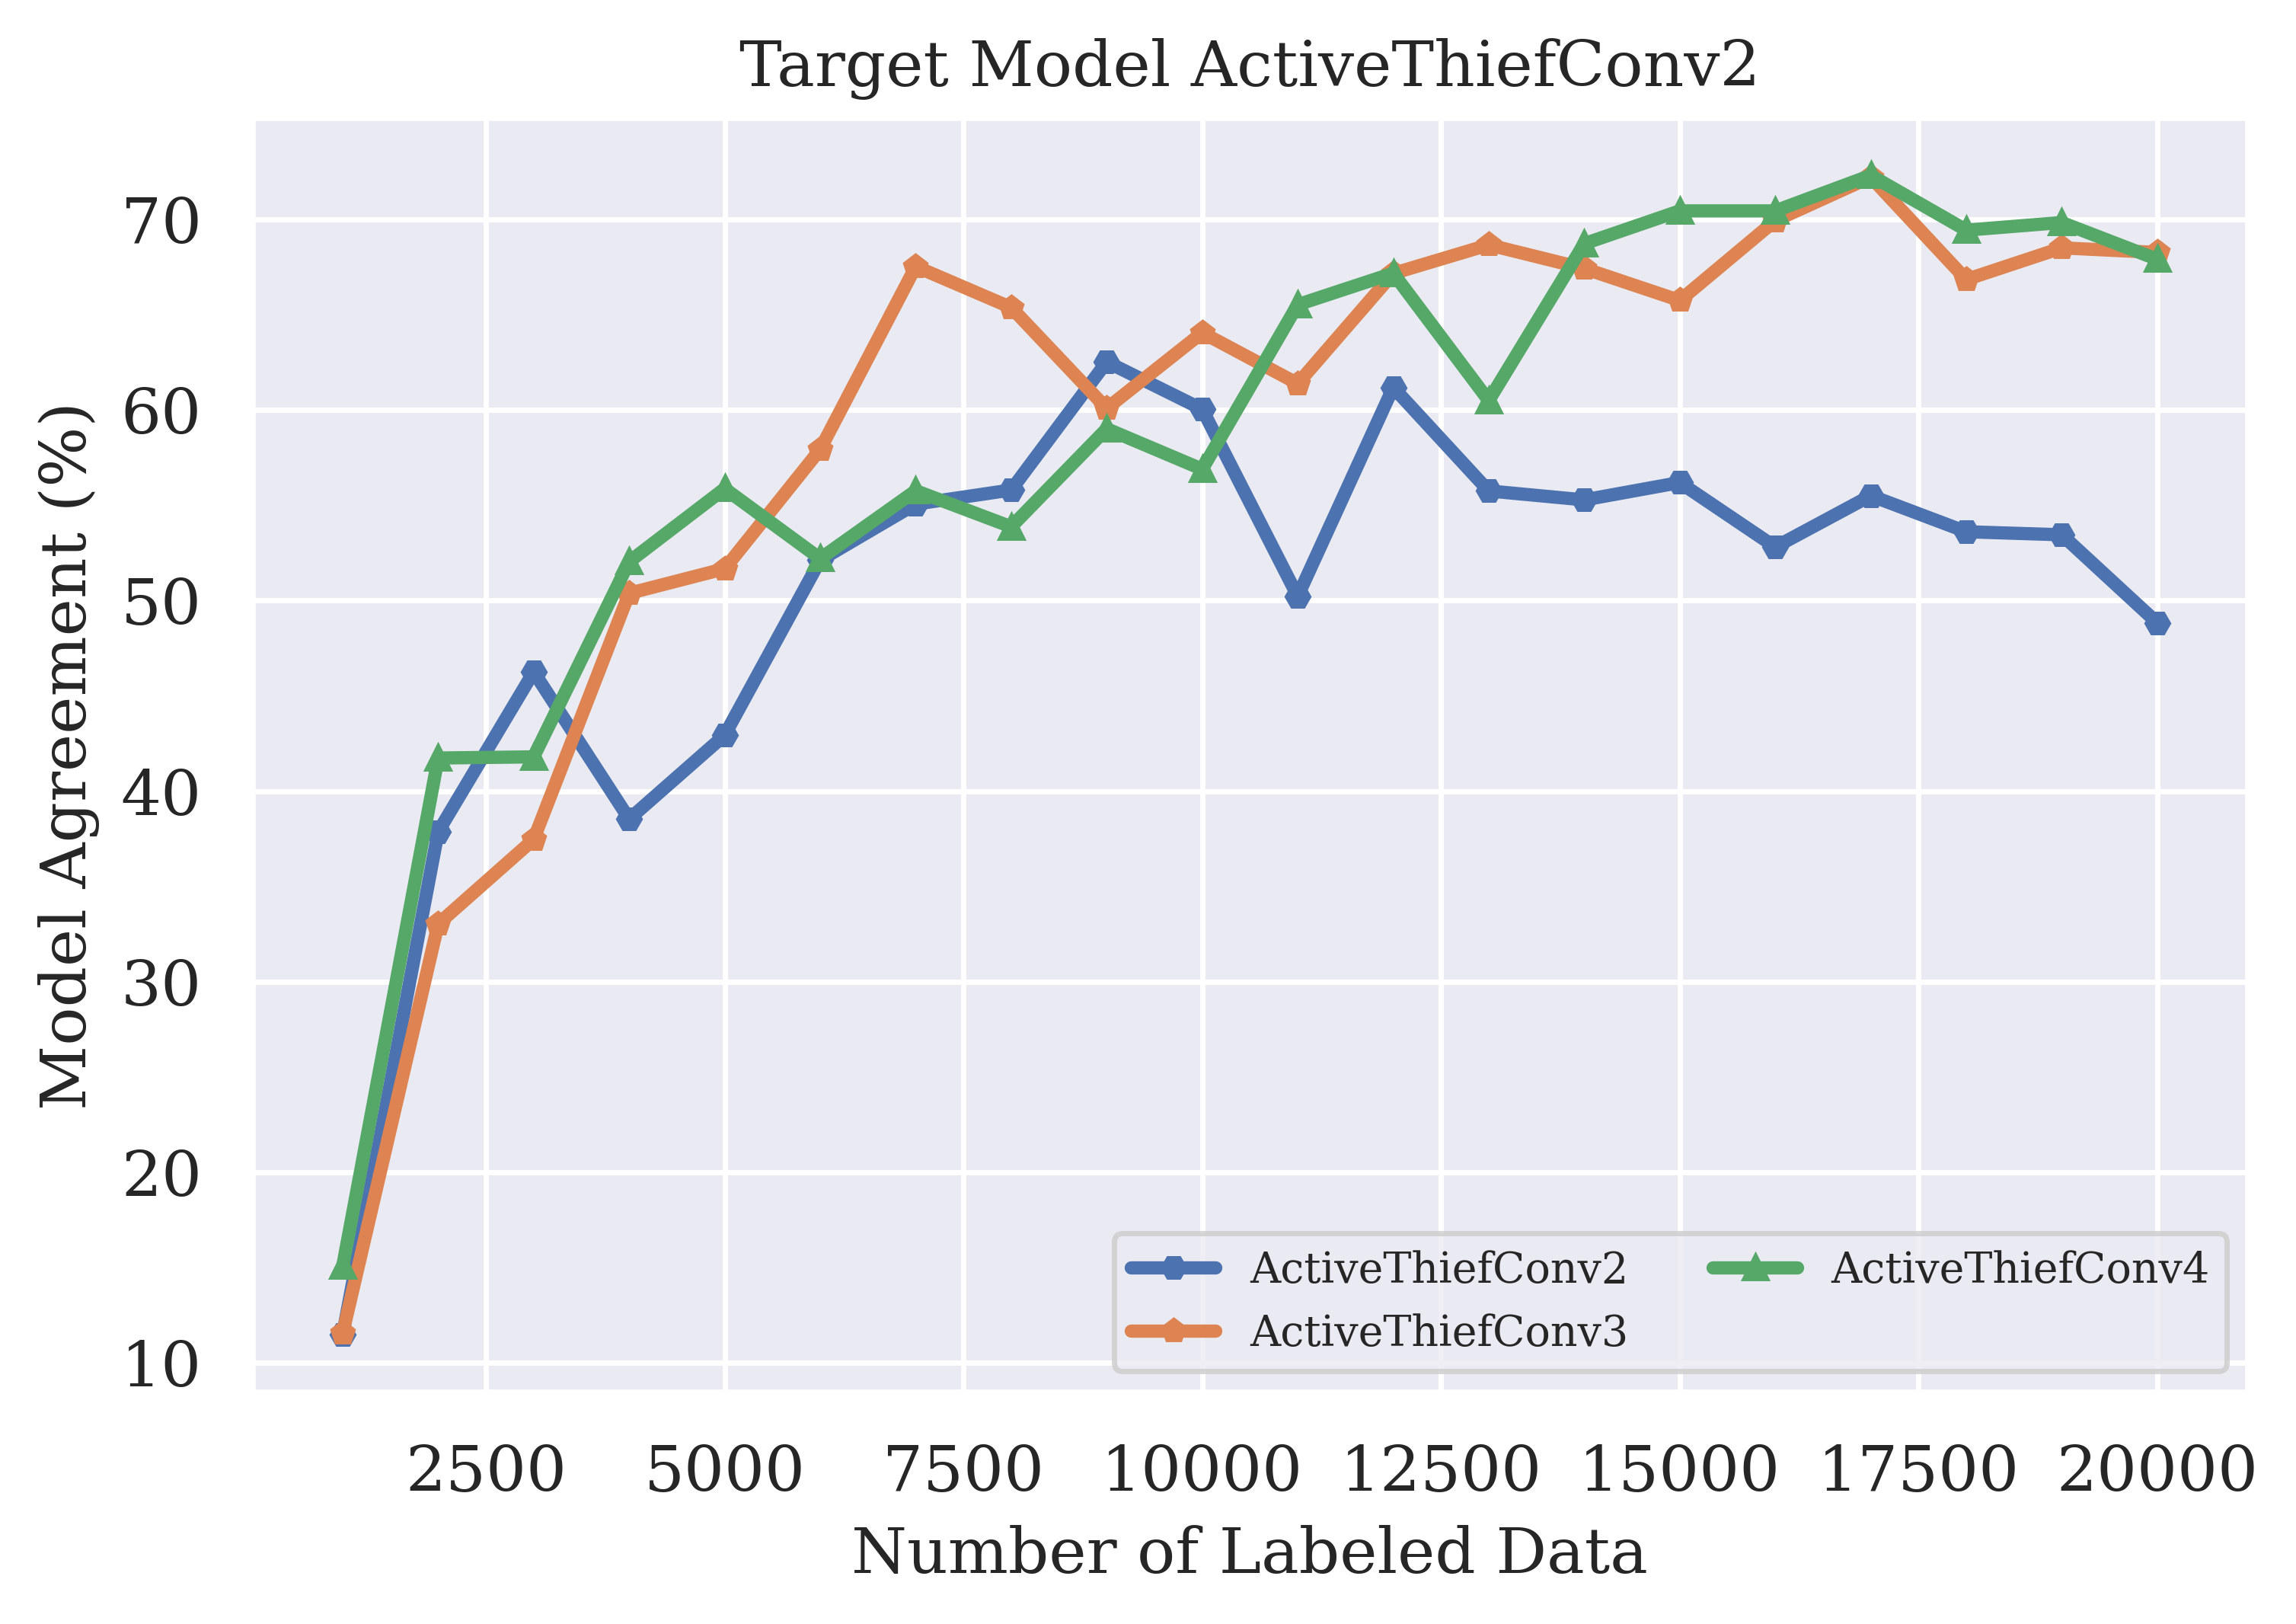
\includegraphics[width=0.32\linewidth]{images/MSInsights/mnist_act2.png} \hfill
    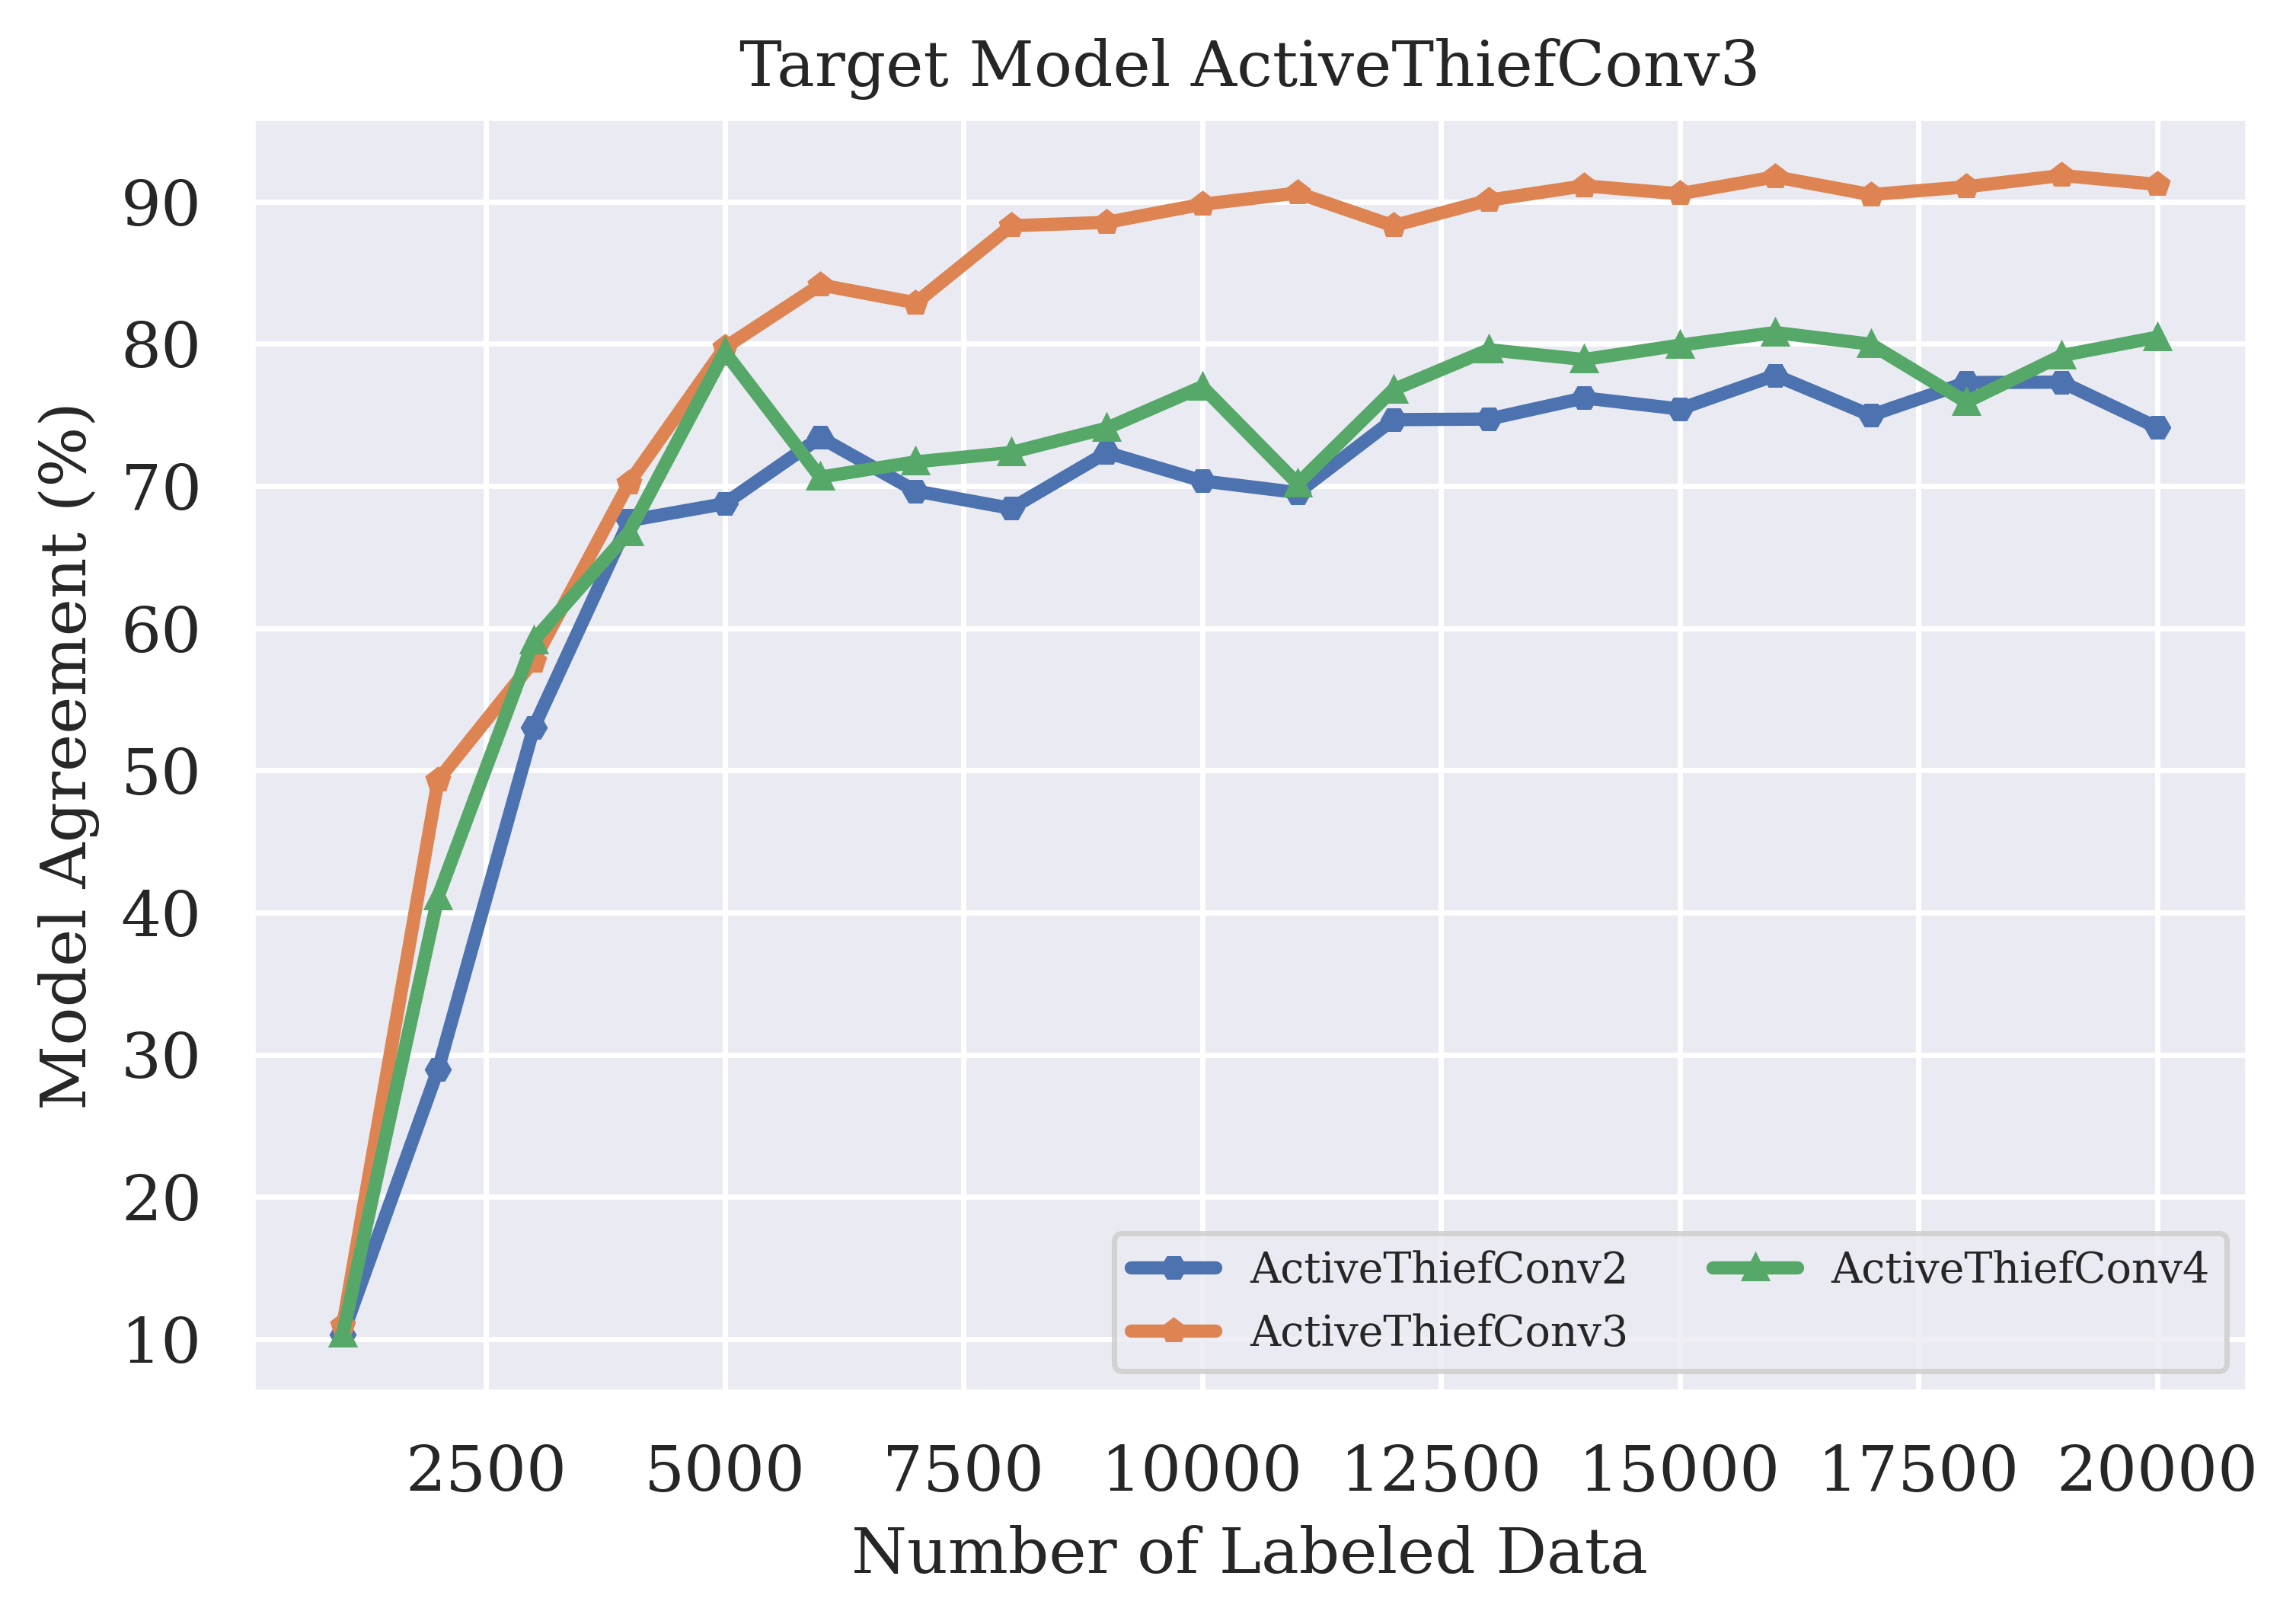
\includegraphics[width=0.32\linewidth]{images/MSInsights/mnist_act3.png} \hfill
    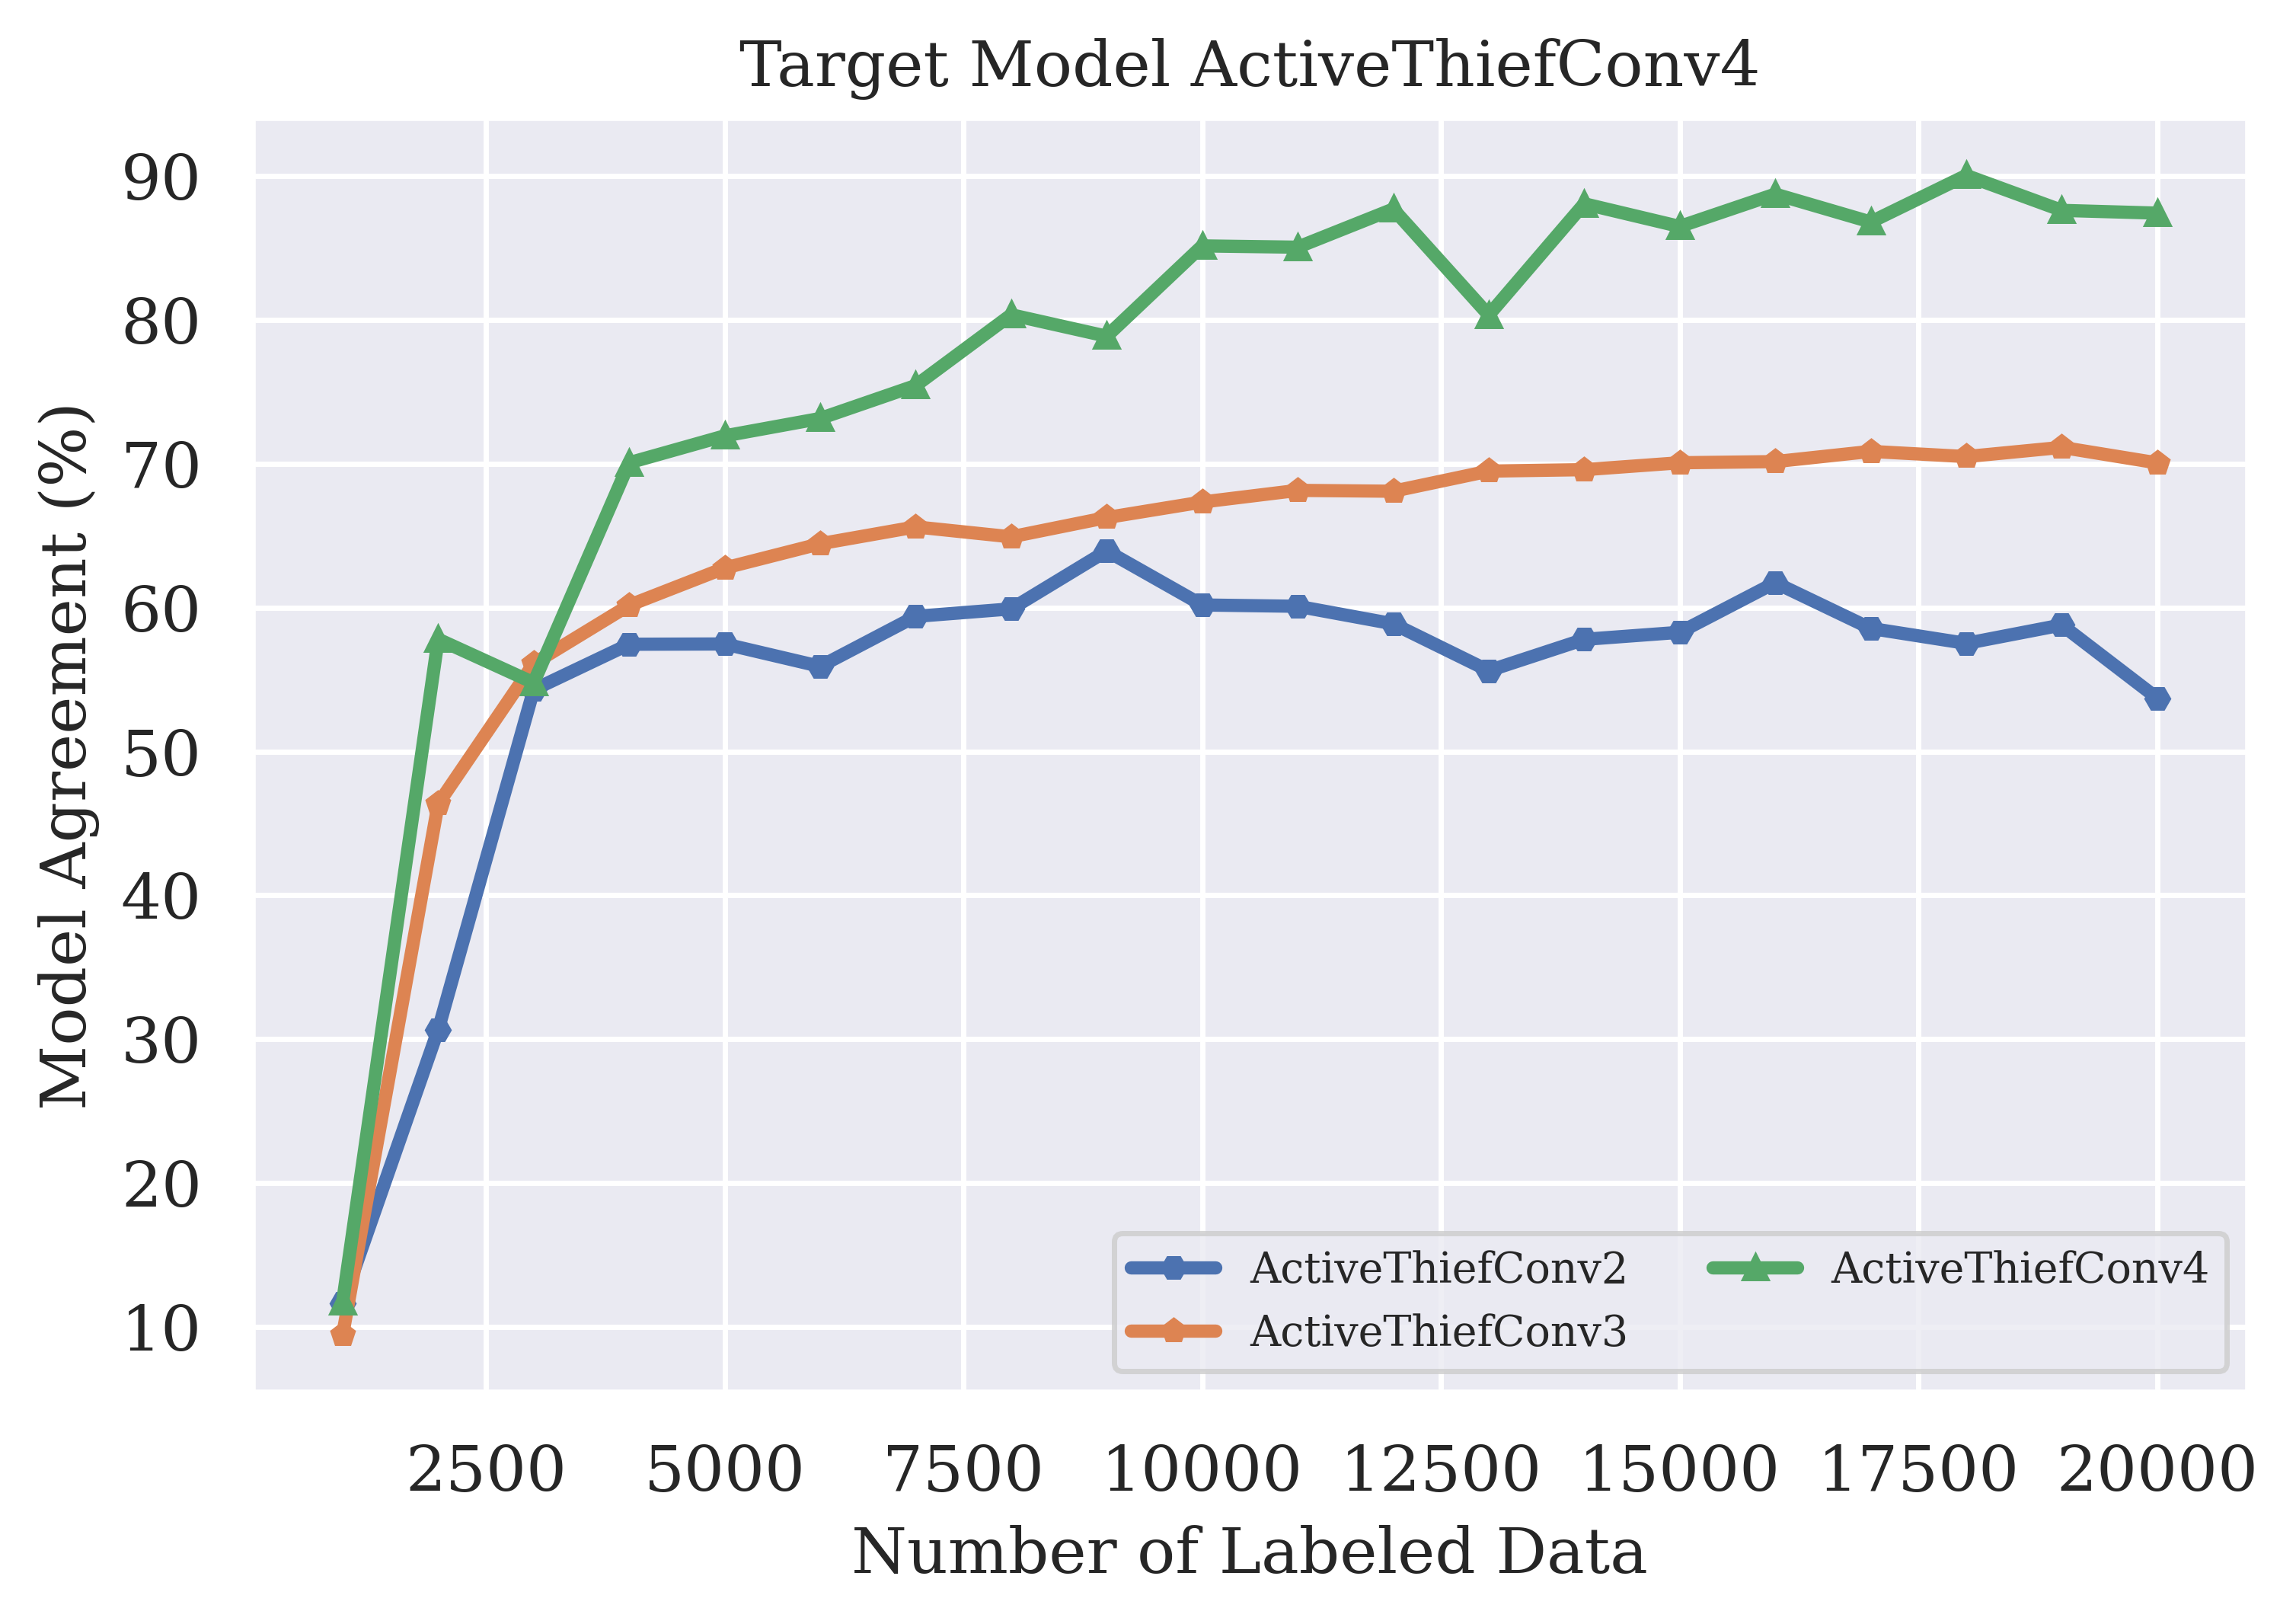
\includegraphics[width=0.32\linewidth]{images/MSInsights/mnist_act4.png}
    \caption{Agreement Progression for Model Stealing using MNIST as a target model dataset}
    \label{fig:MNISTmodelComp}
\end{figure}

\begin{figure}[!htb]
    \centering
    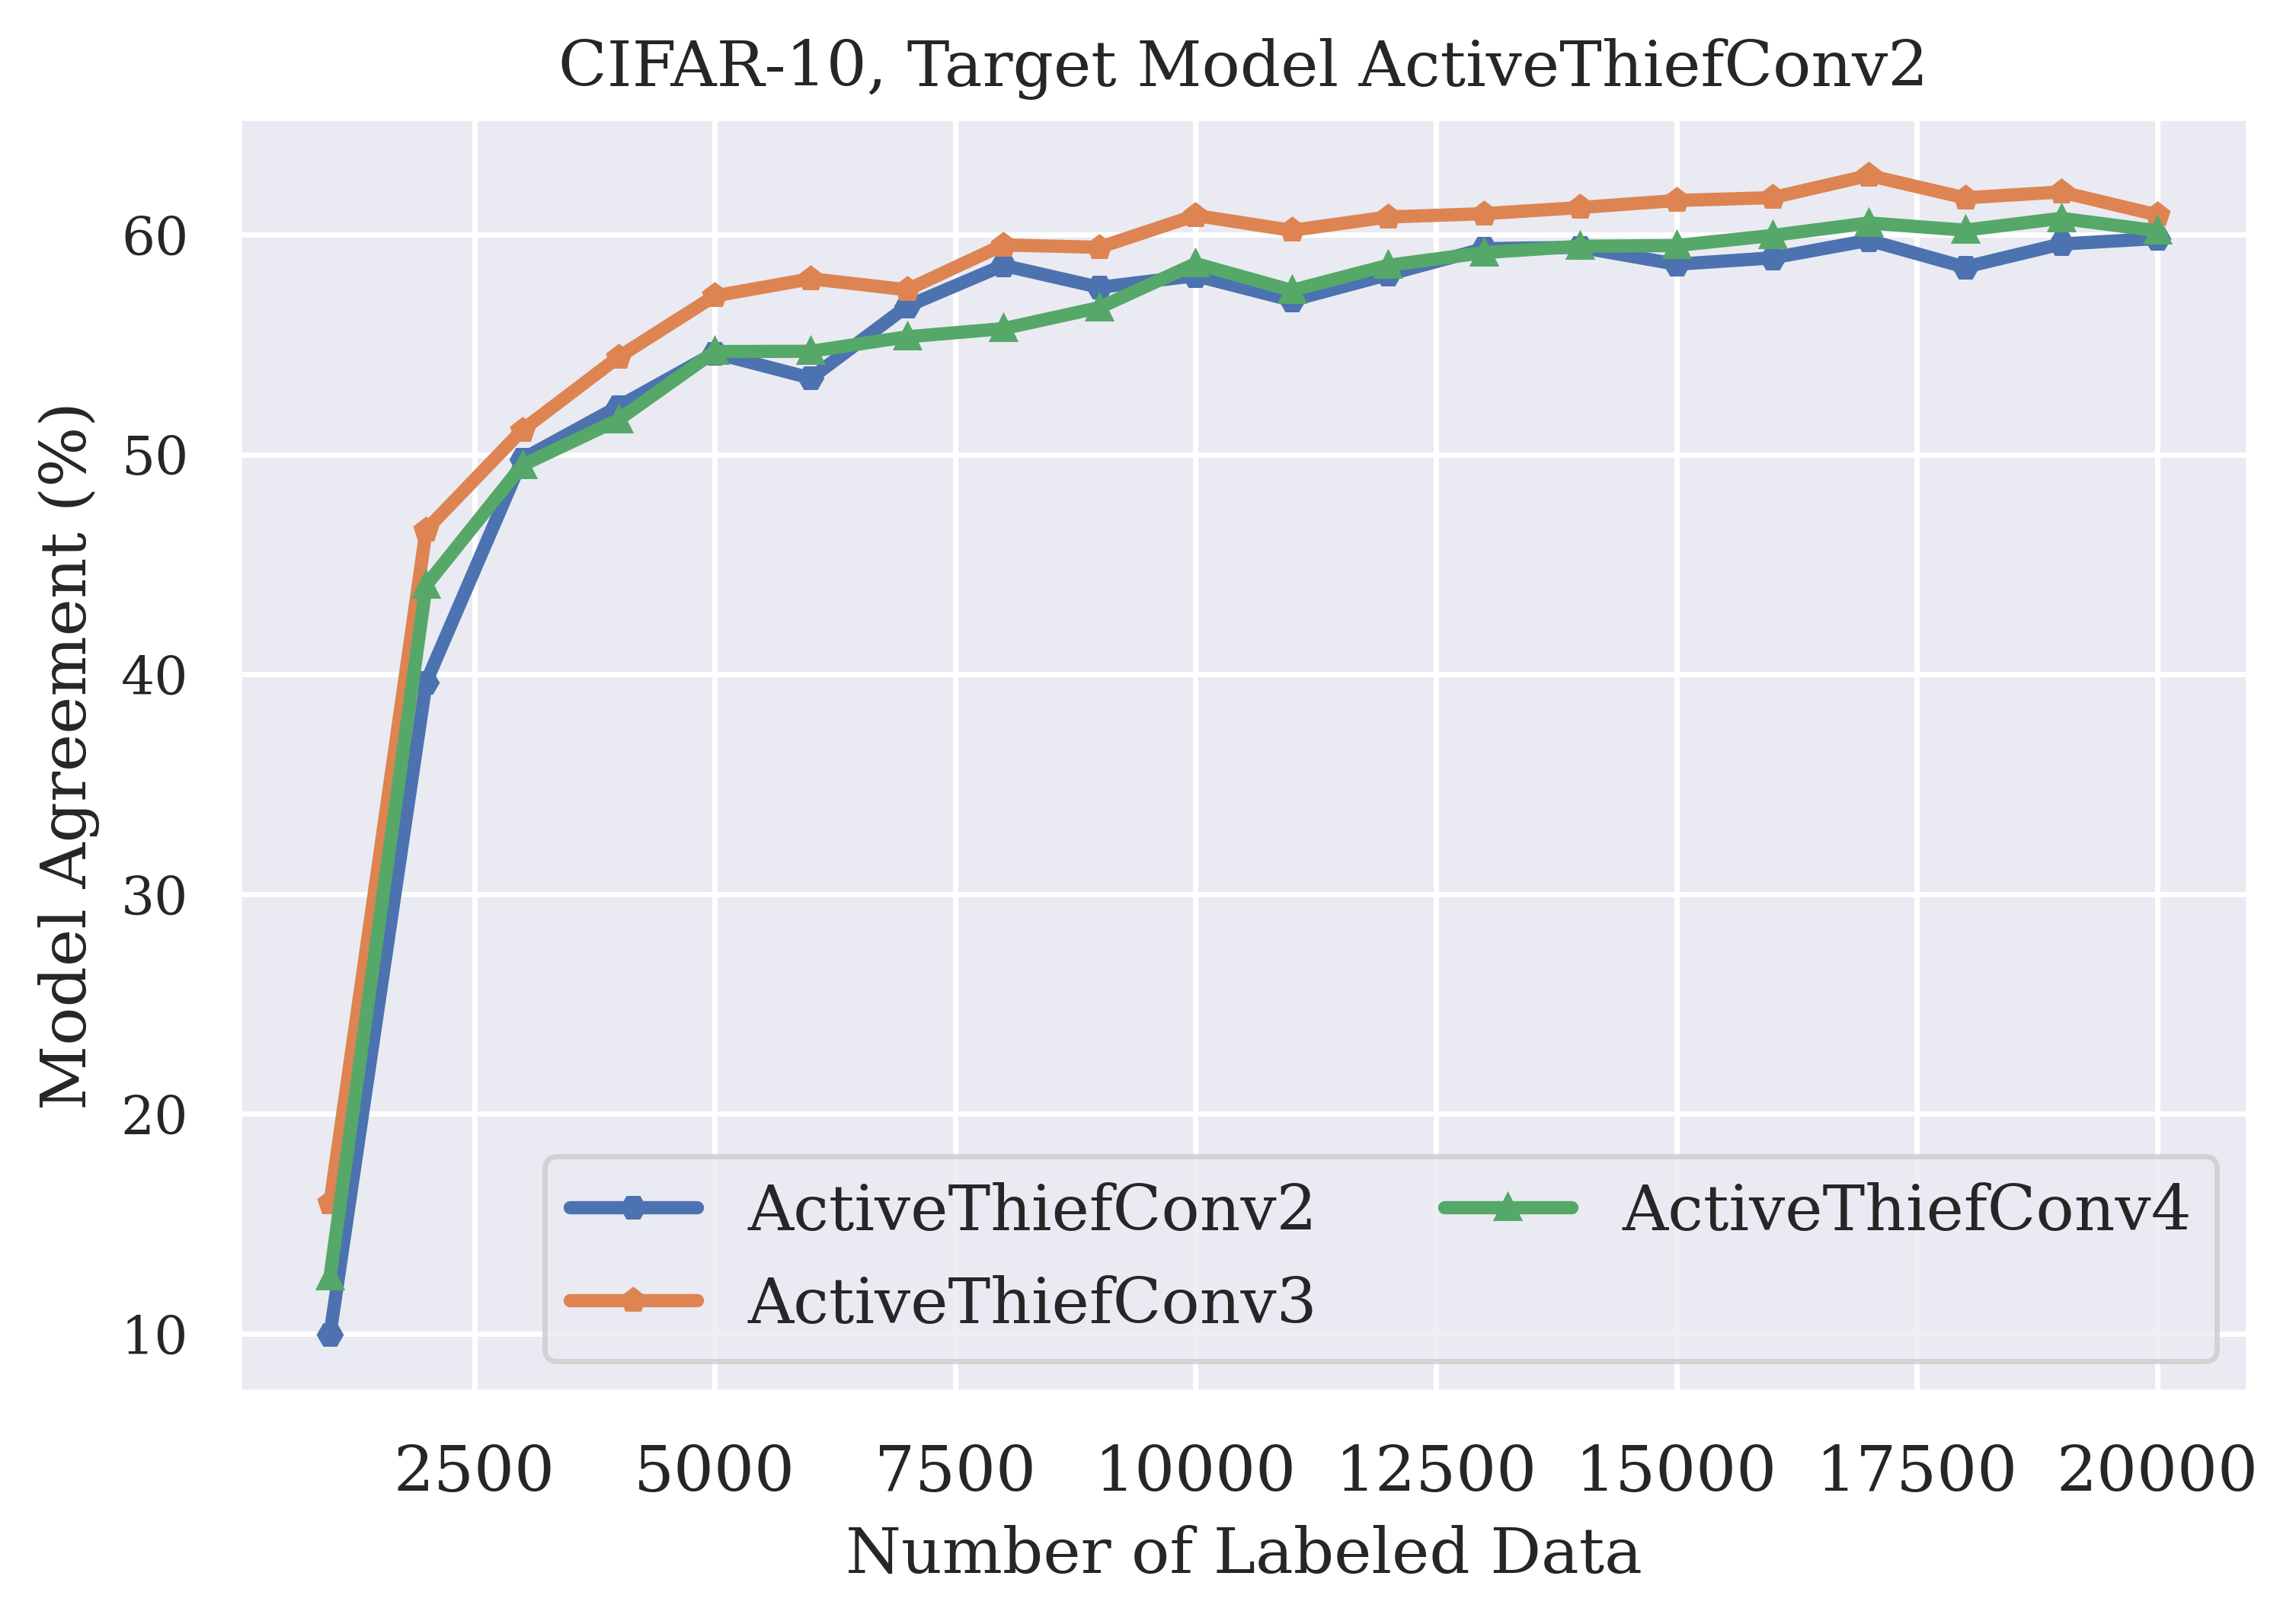
\includegraphics[width=0.32\linewidth]{images/MSInsights/cifar_act2.png} \hfill
    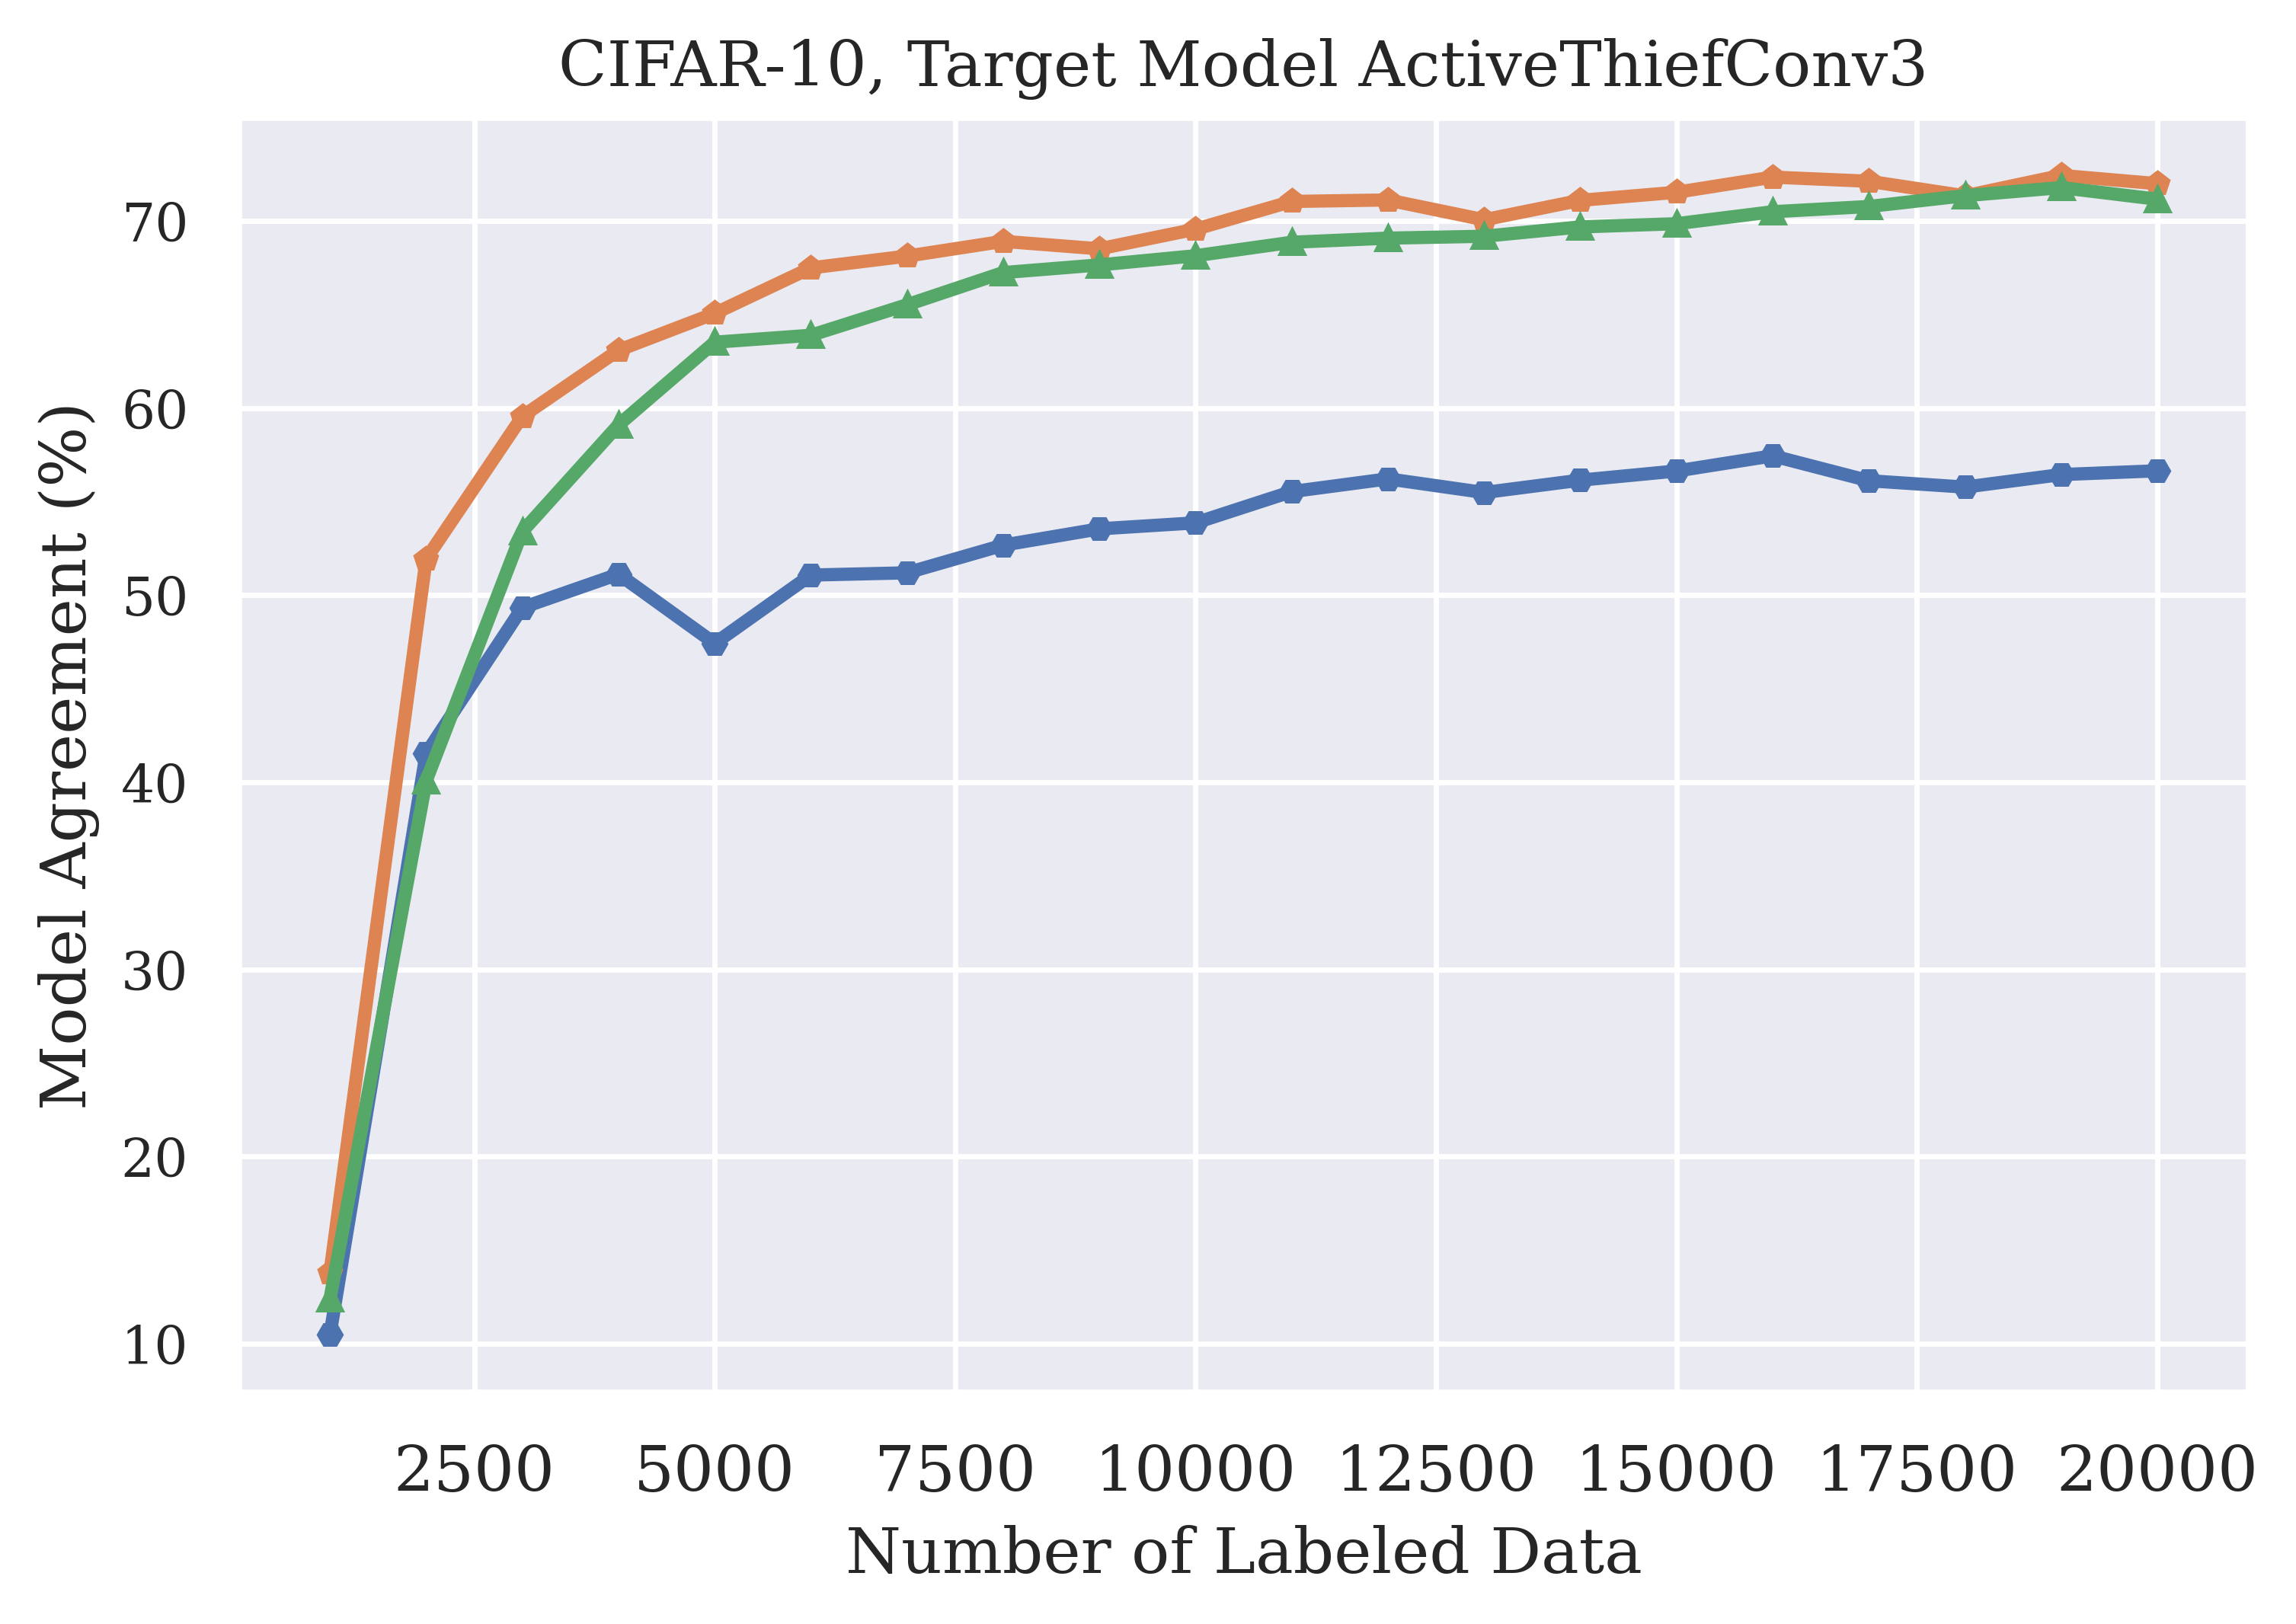
\includegraphics[width=0.32\linewidth]{images/MSInsights/cifar_act3.png} \hfill
    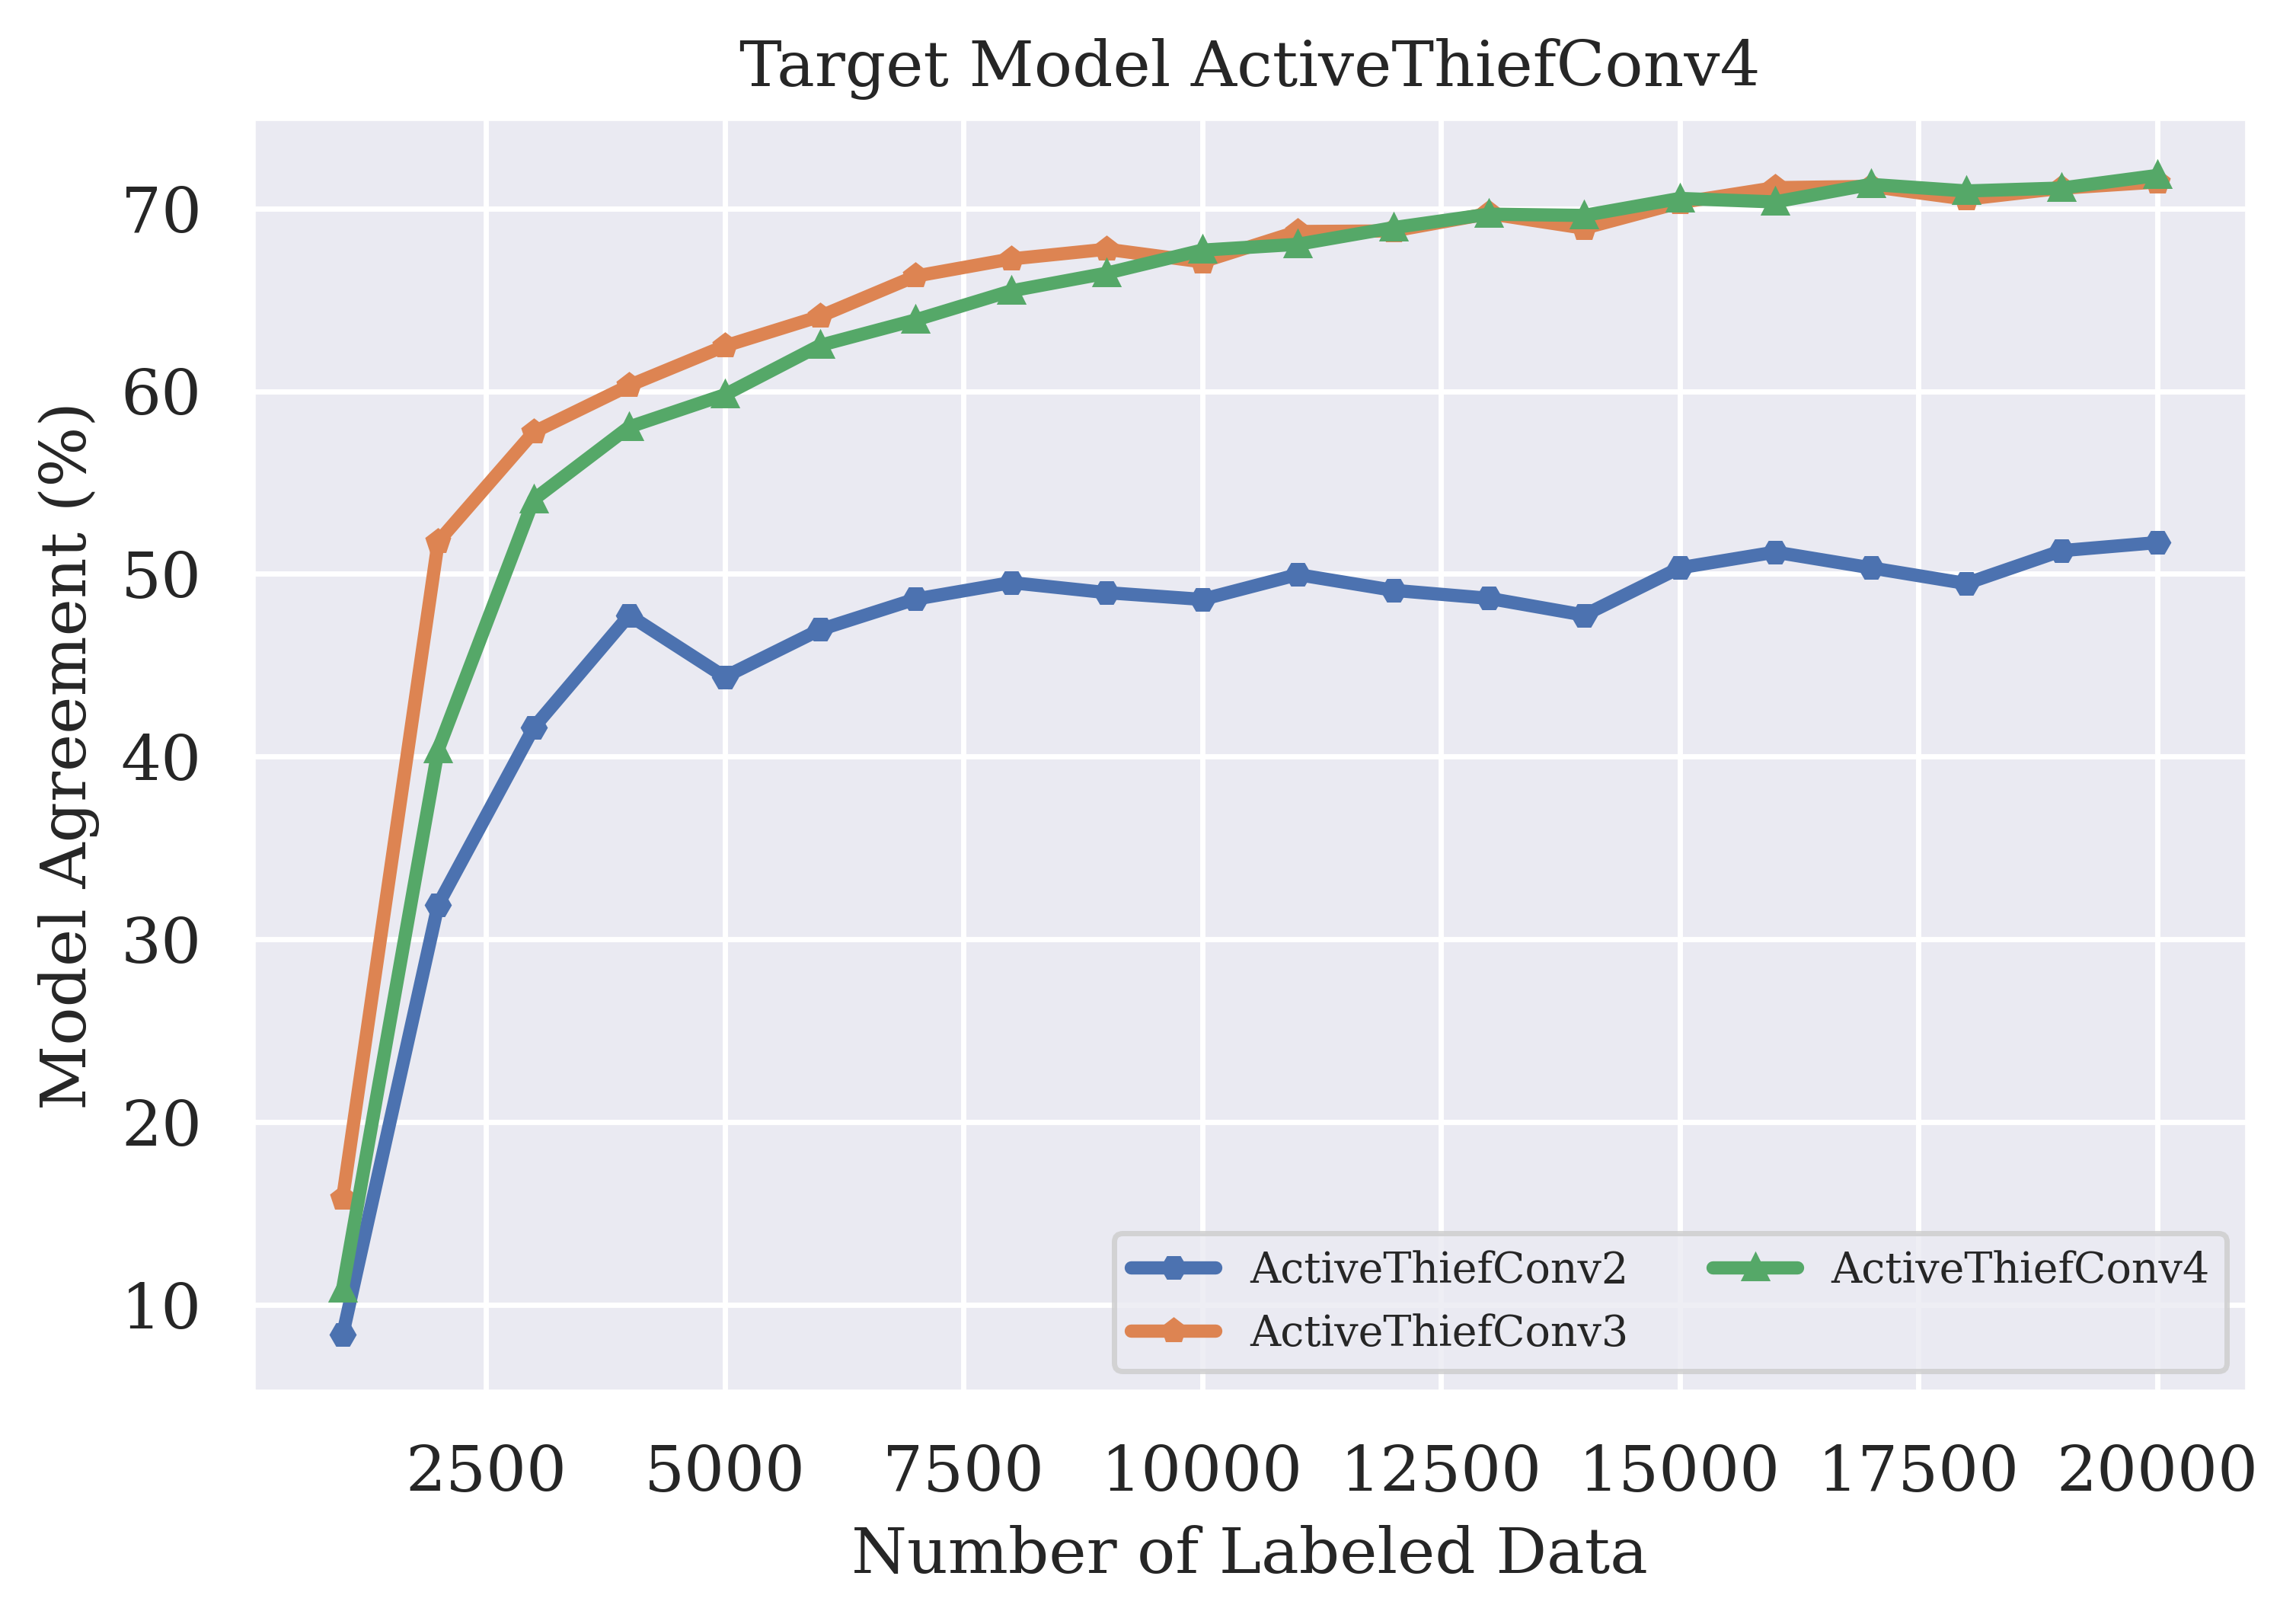
\includegraphics[width=0.32\linewidth]{images/MSInsights/cifar_act4.png}
    \caption{Agreement progression for model stealing using CIFAR-10 as a target model dataset}
    \label{fig:CIFAR10modelComp}
\end{figure}


After evaluating the influence of the target and substitute model architecture on the success of the model stealing attack, we now evaluate how the thief dataset effects Model Stealing Attacks. Our motivation for this experiment is that Pal et al. 
mention having tested CIFAR-10 as a thief dataset with without success. We perform a model stealing attack using ActiveThiefConv3 as the target and substitute model and CoreSet with batch size 2000 as our Active Learning strategy. The total query budget
is 20000. We used MNIST as the target model dataset and change between Small ImageNet, Tiny ImageNet and CIFAR-10 as our thief datasets. The results of this experiment can be seen in figure \ref{fig:Evaluation:Results:CAL:EffectDataset}. While the model agreement 
increases throughout the experiment when using Small ImageNet, the model agreement for Tiny ImageNet plateaus after just 3 iterations at 20\%. Model Stealing with CIFAR-10 yields the best results, however. At the end of the experiment, the setup with CIFAR-10 as 
the thief dataset achieves a Model Agreement which is 5 percentage points higher than the setup with Small Imagenet as the thief dataset. \par

\begin{figure}[h]
    \centering
    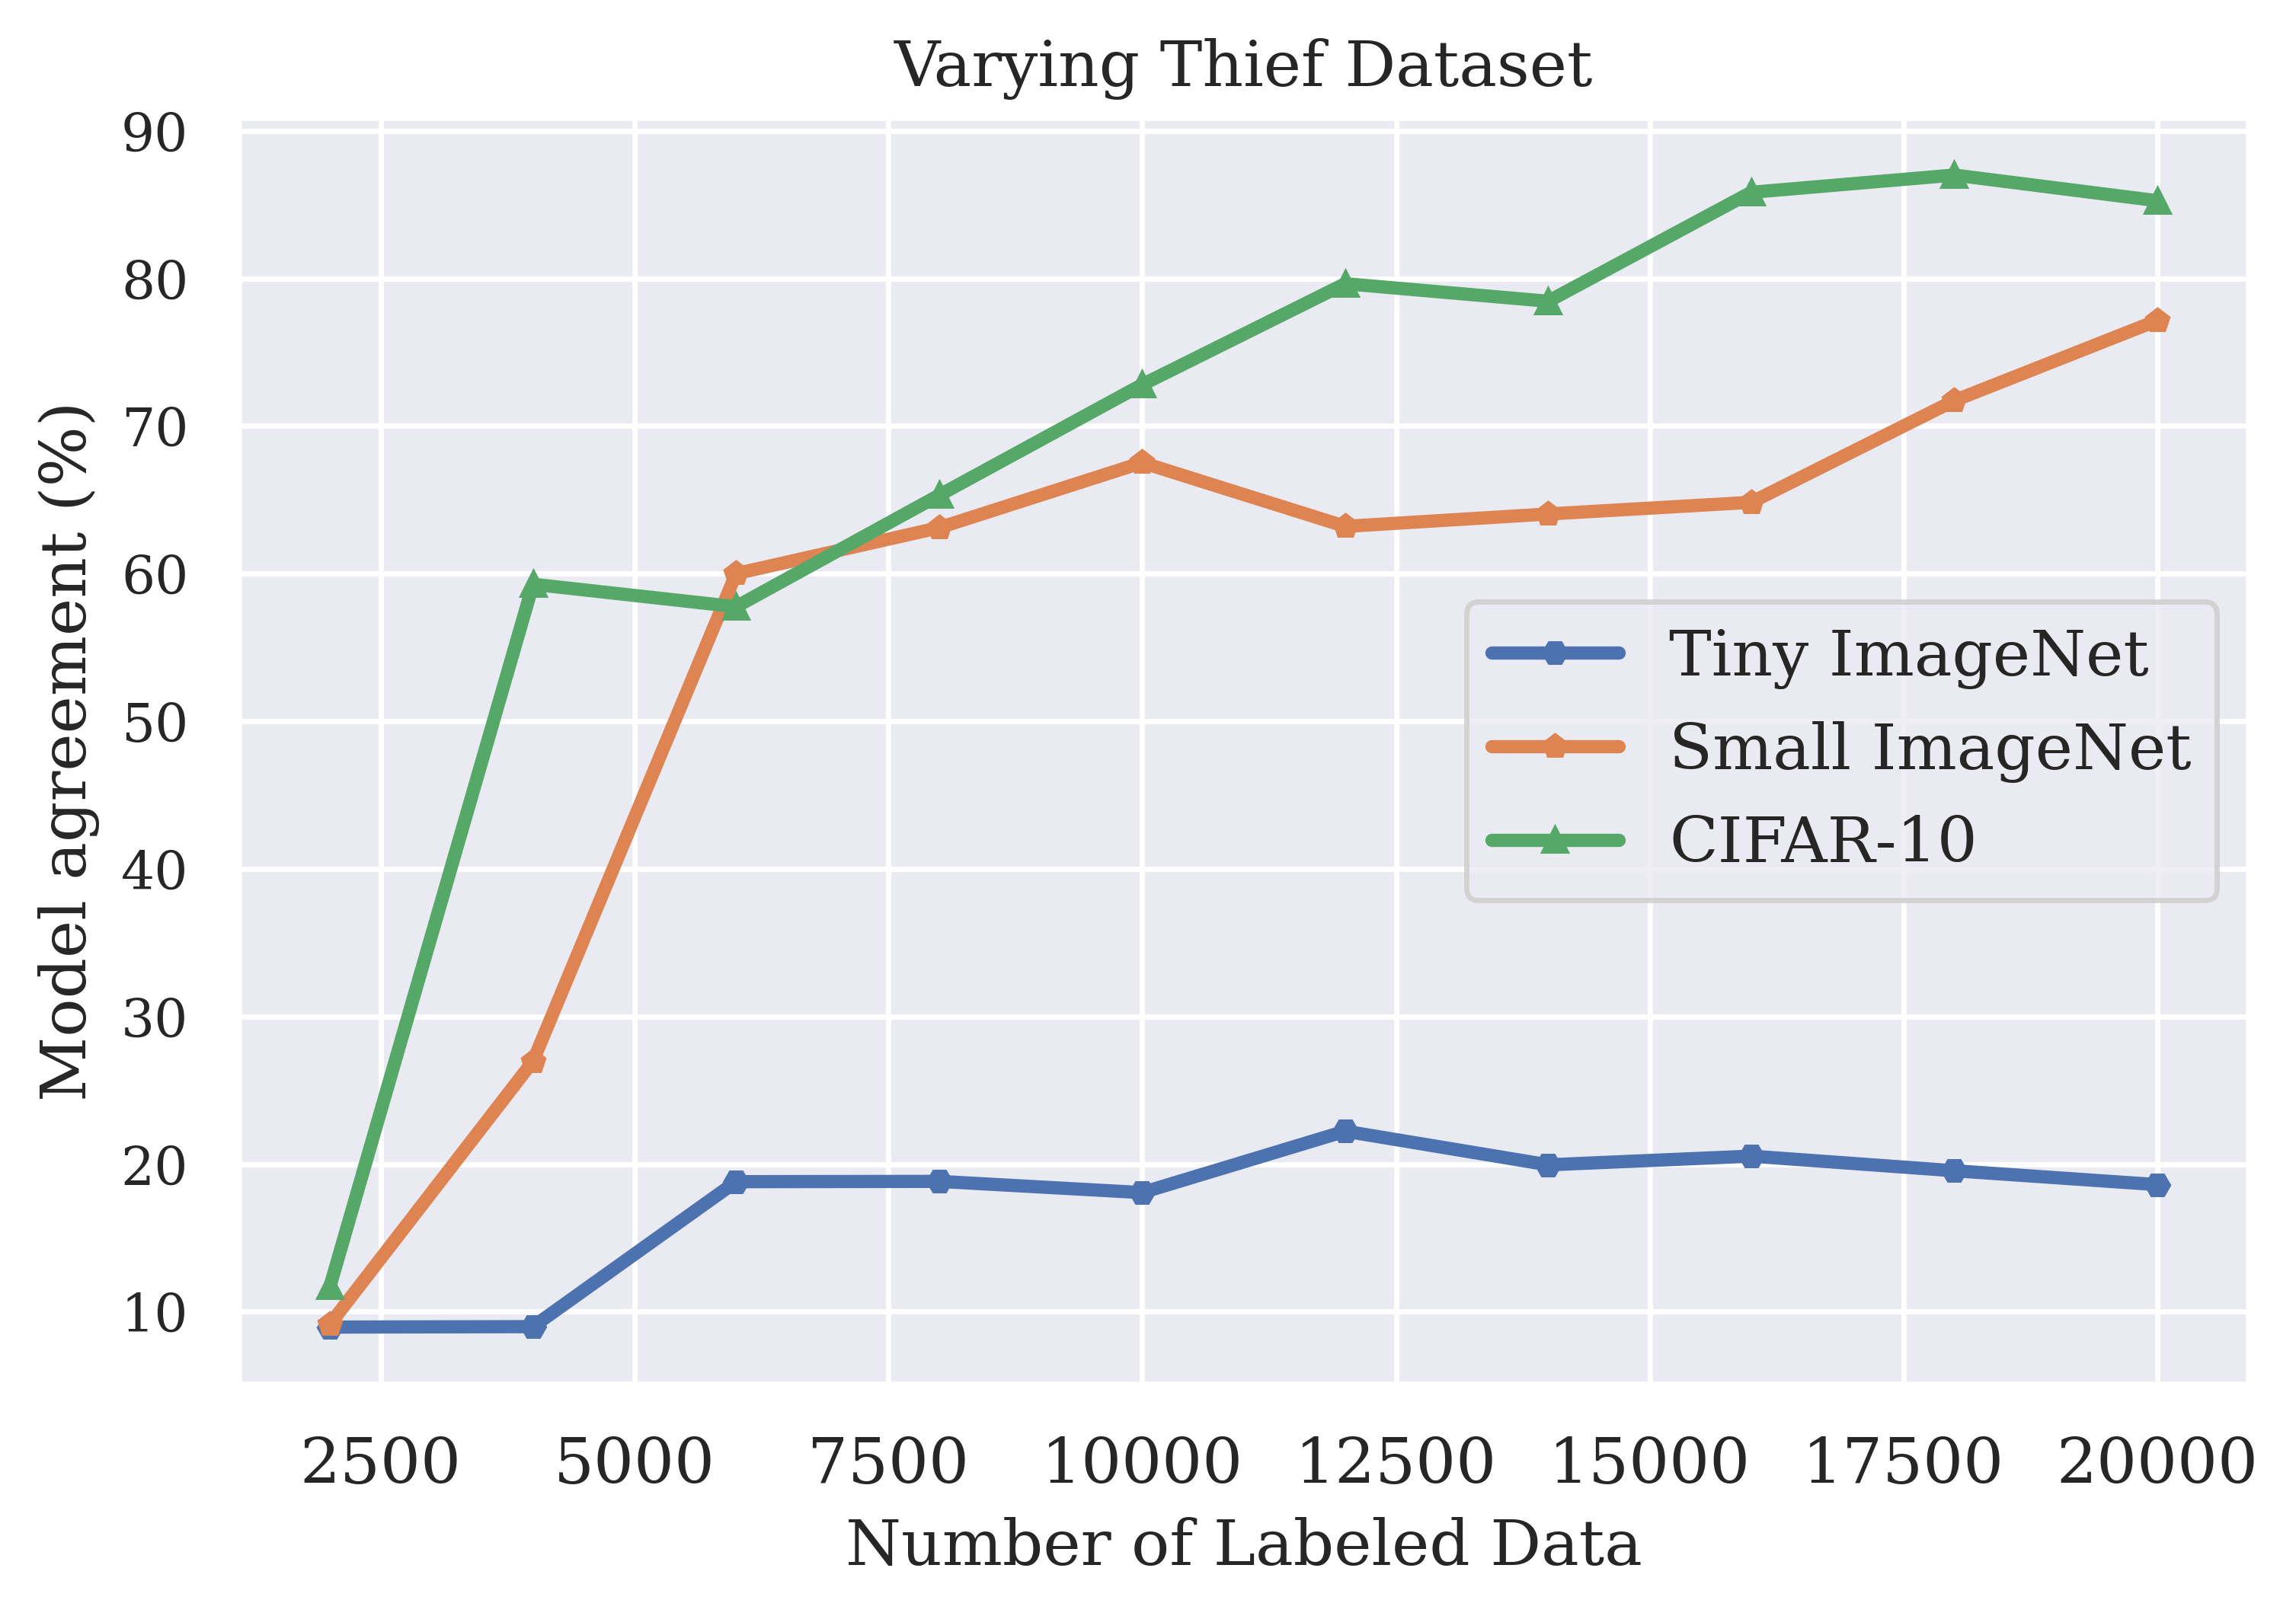
\includegraphics[width=0.8\linewidth]{images/results_CALMS/effect_dataset.png}
    \caption[Effect of Thief Dataset choice on the success of Model Stealing Attacks]{Comparison of Model Agreement when performing a model stealing attack using the datasets Tiny Imagenet, Small ImageNet and CIFAR-10. We perform Active Learning using the 
    straegy CoreSet with a batch size of 2000 for the experiments. The target model dataset used is MNIST.}
    \label{fig:Evaluation:Results:CAL:EffectDataset}
\end{figure}



\subsection{Continual Active Learning for Model Stealing}
\label{sec:Appendix:CALMS}
This section contains plots of the full runs of all experiments in section \ref{sec:Evaluation:Results:MS:CAL}.

\subsubsection{MNIST}
\label{sec:Appendix:CALMS:MNIST}
In this section, we present the full runs of all experiments which involve Continual Active Learning using MNIST as a Target Model Dataset.

\begin{figure}[!htb]
    \centering
    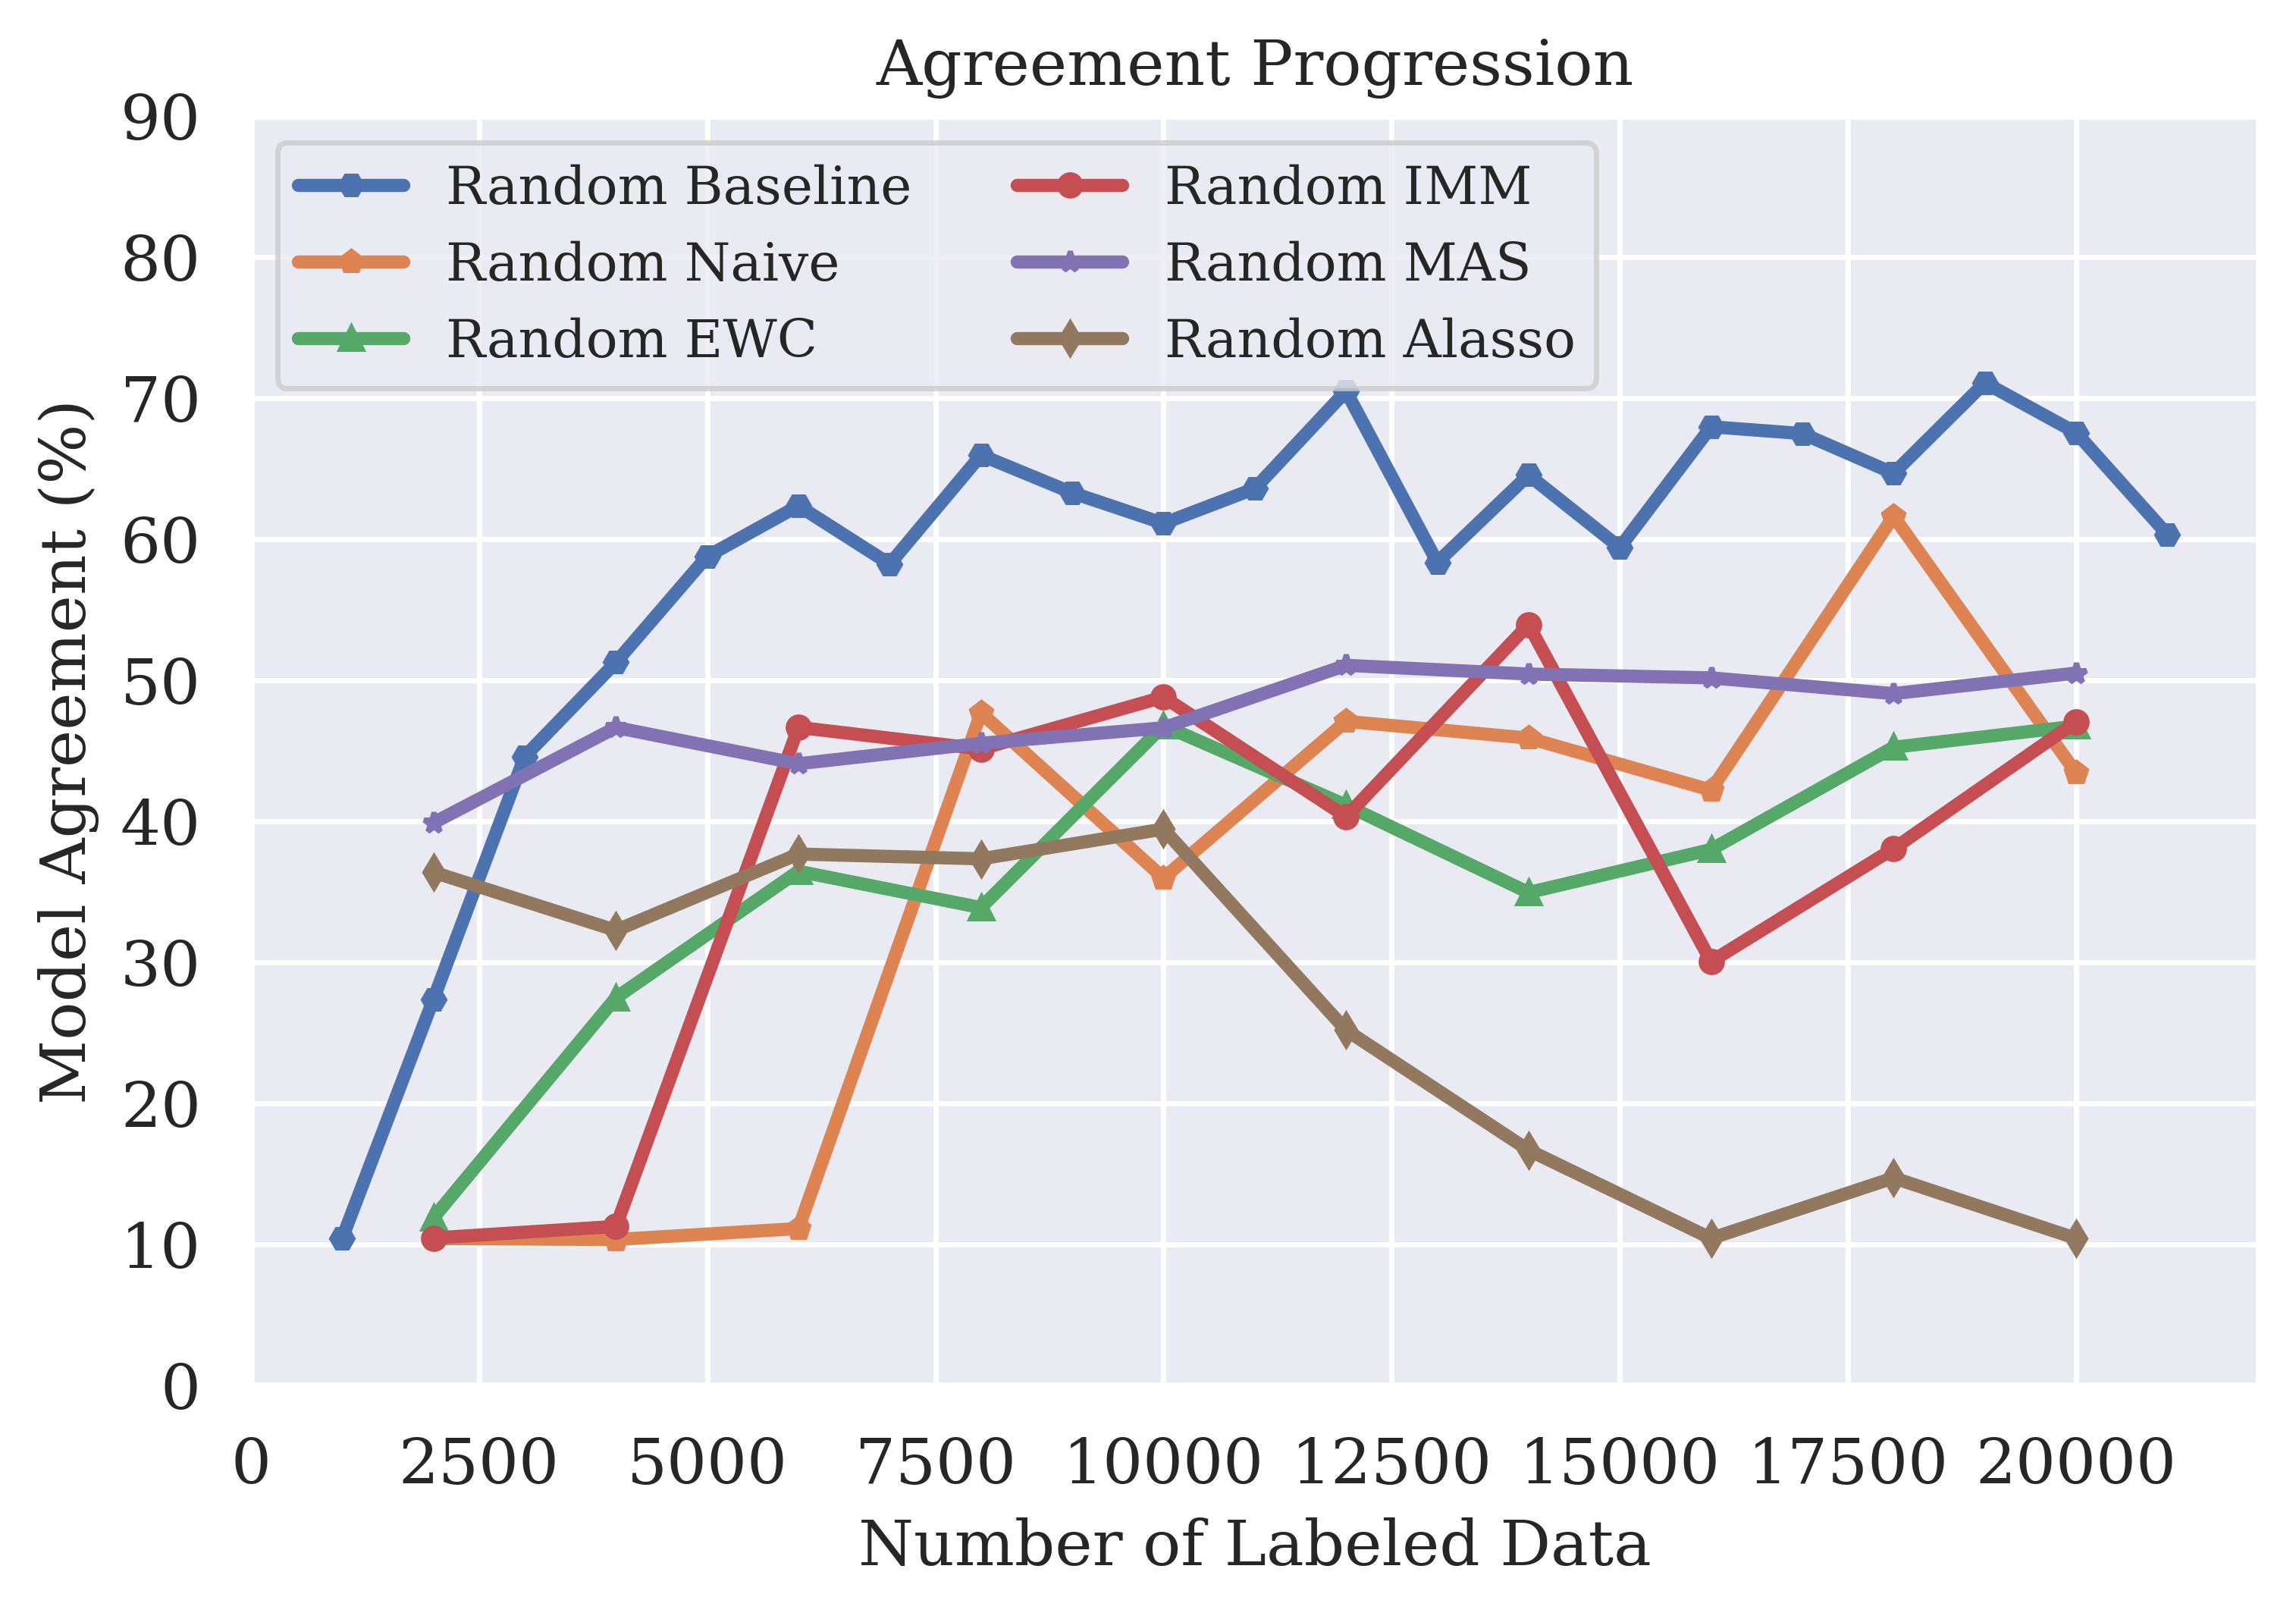
\includegraphics[width=0.48\linewidth]{images/results_CALMS/mnist_label_random.png} \hfill
    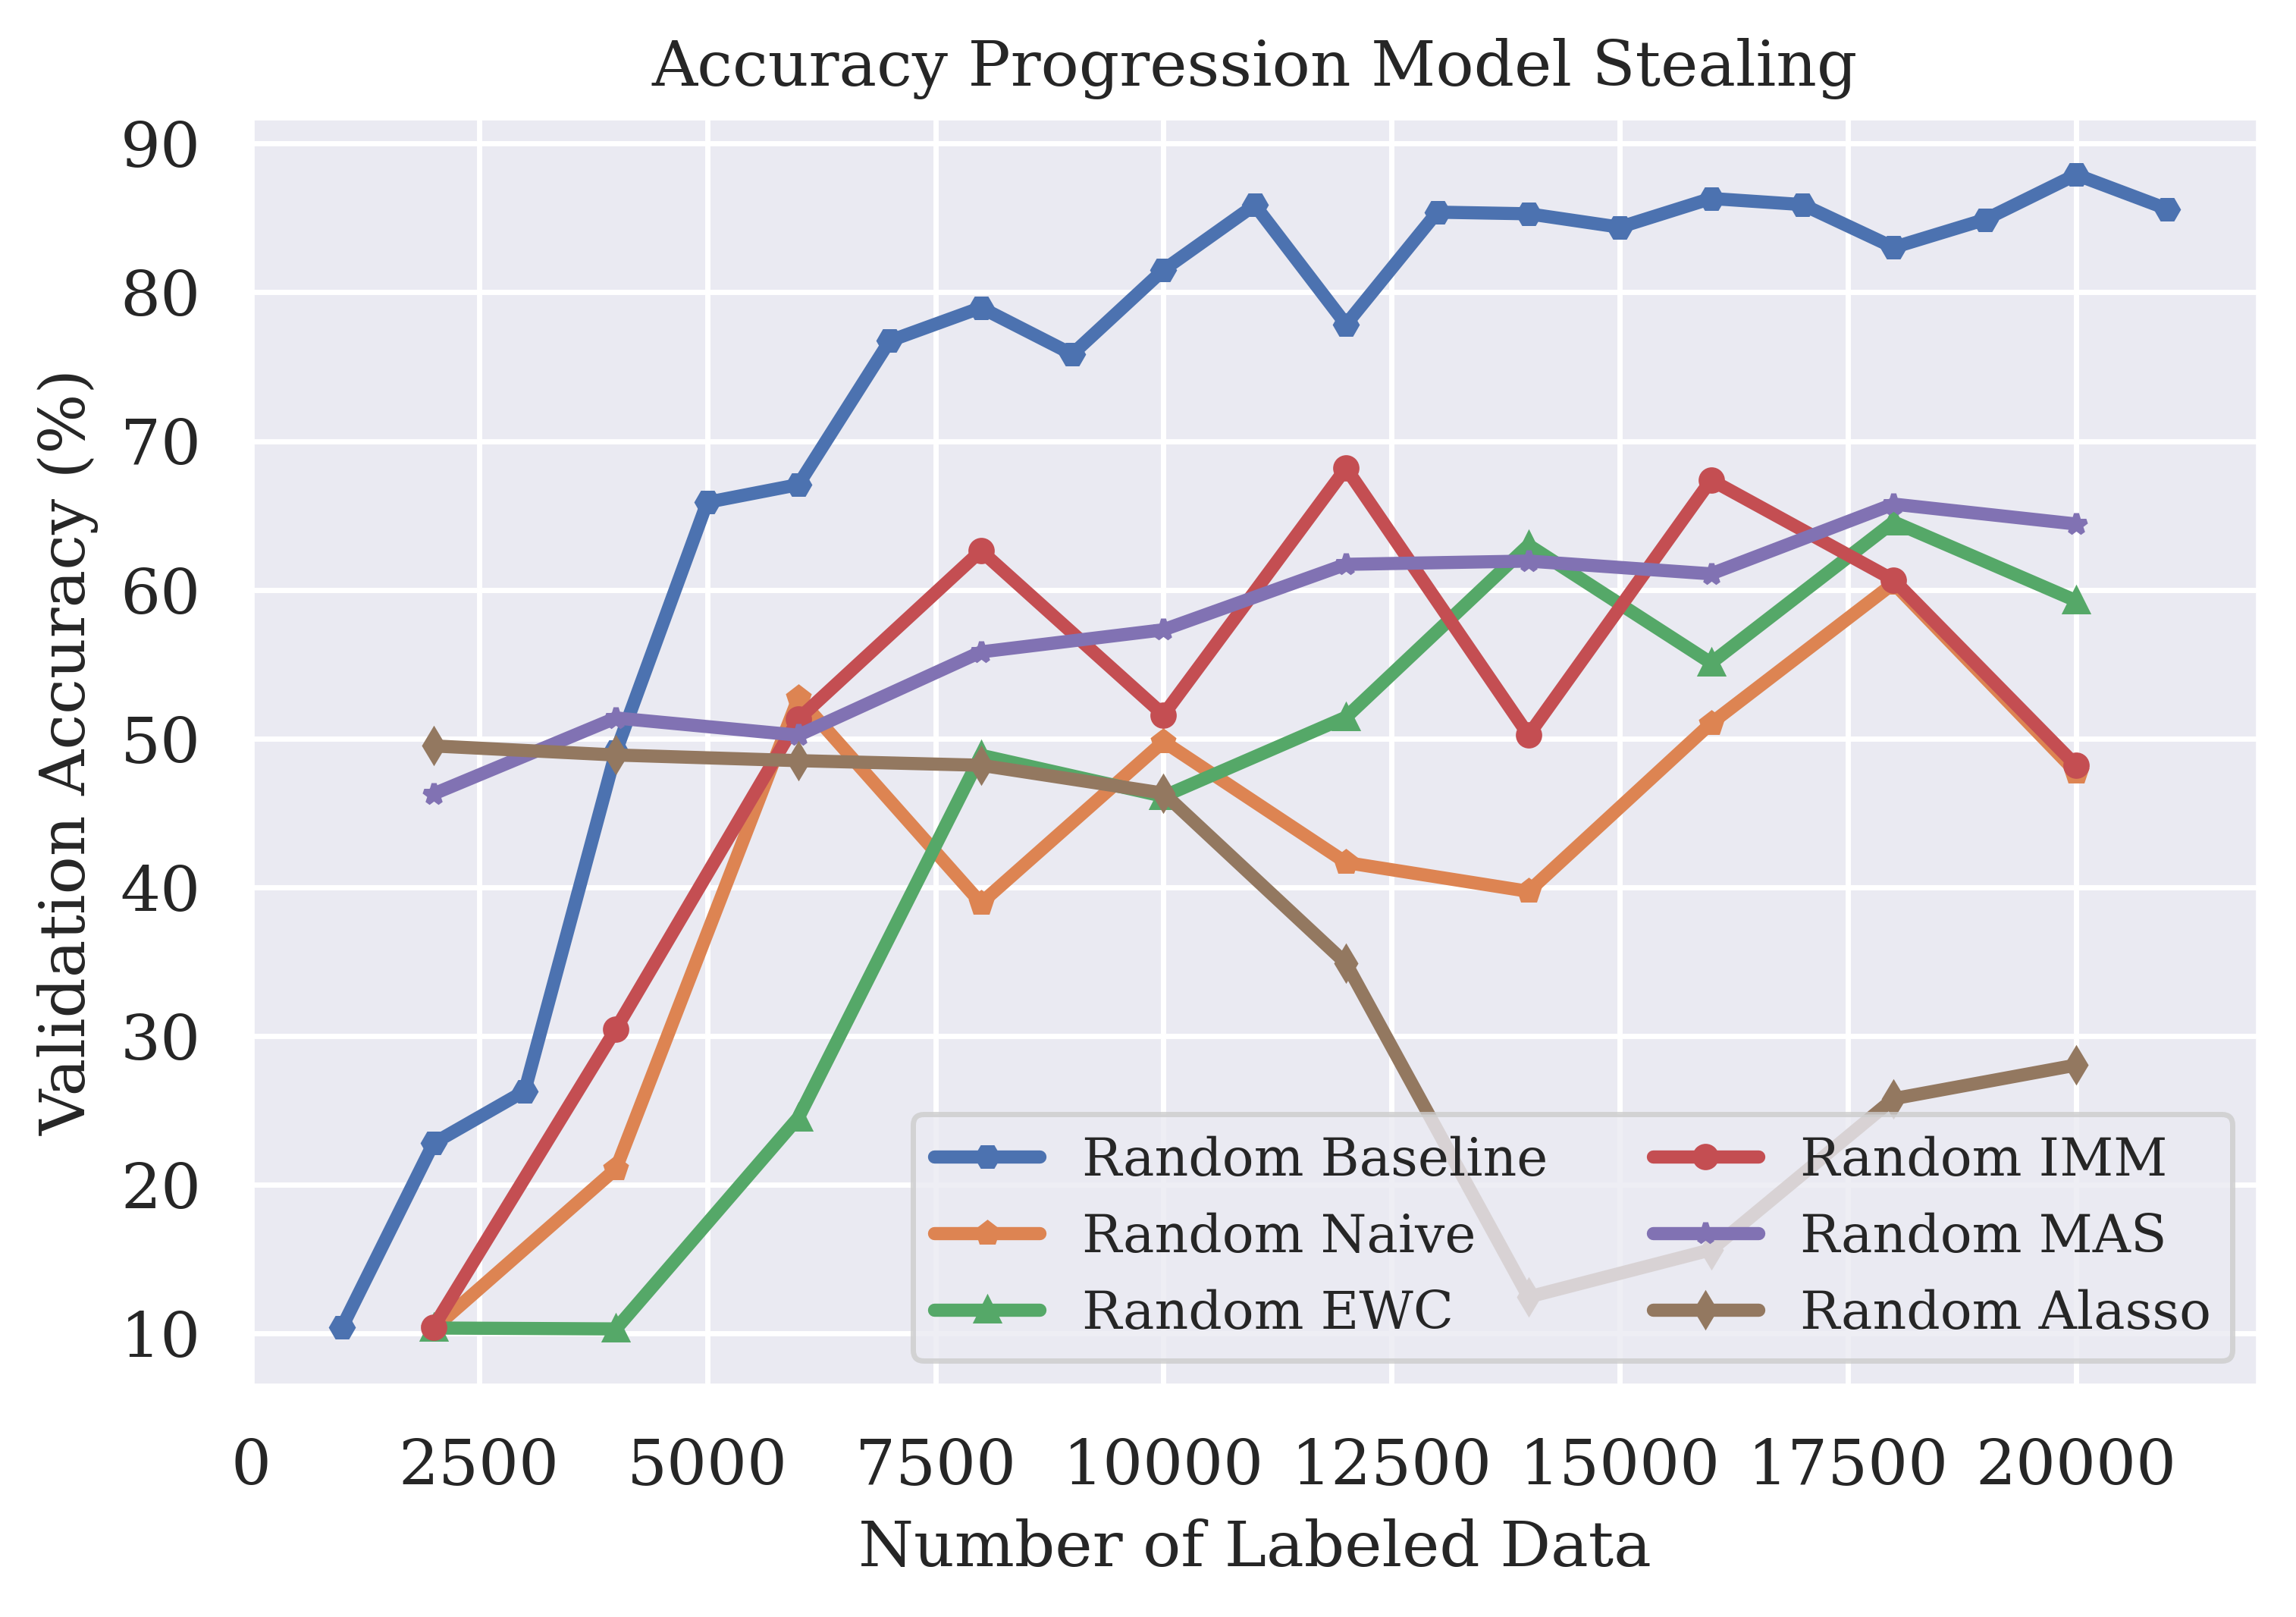
\includegraphics[width=0.48\linewidth]{images/results_CALMS/mnist_softmax_random.png}
    \caption{Agreement Comparison for Model Stealing on MNIST using the softmax output and the Active Learning strategy Random. Left: Training with predicted class label,
    Right: Training with softmax output}
    \label{fig:CALMSMNISTRandom}
\end{figure}

\begin{figure}[!htb]
    \centering
    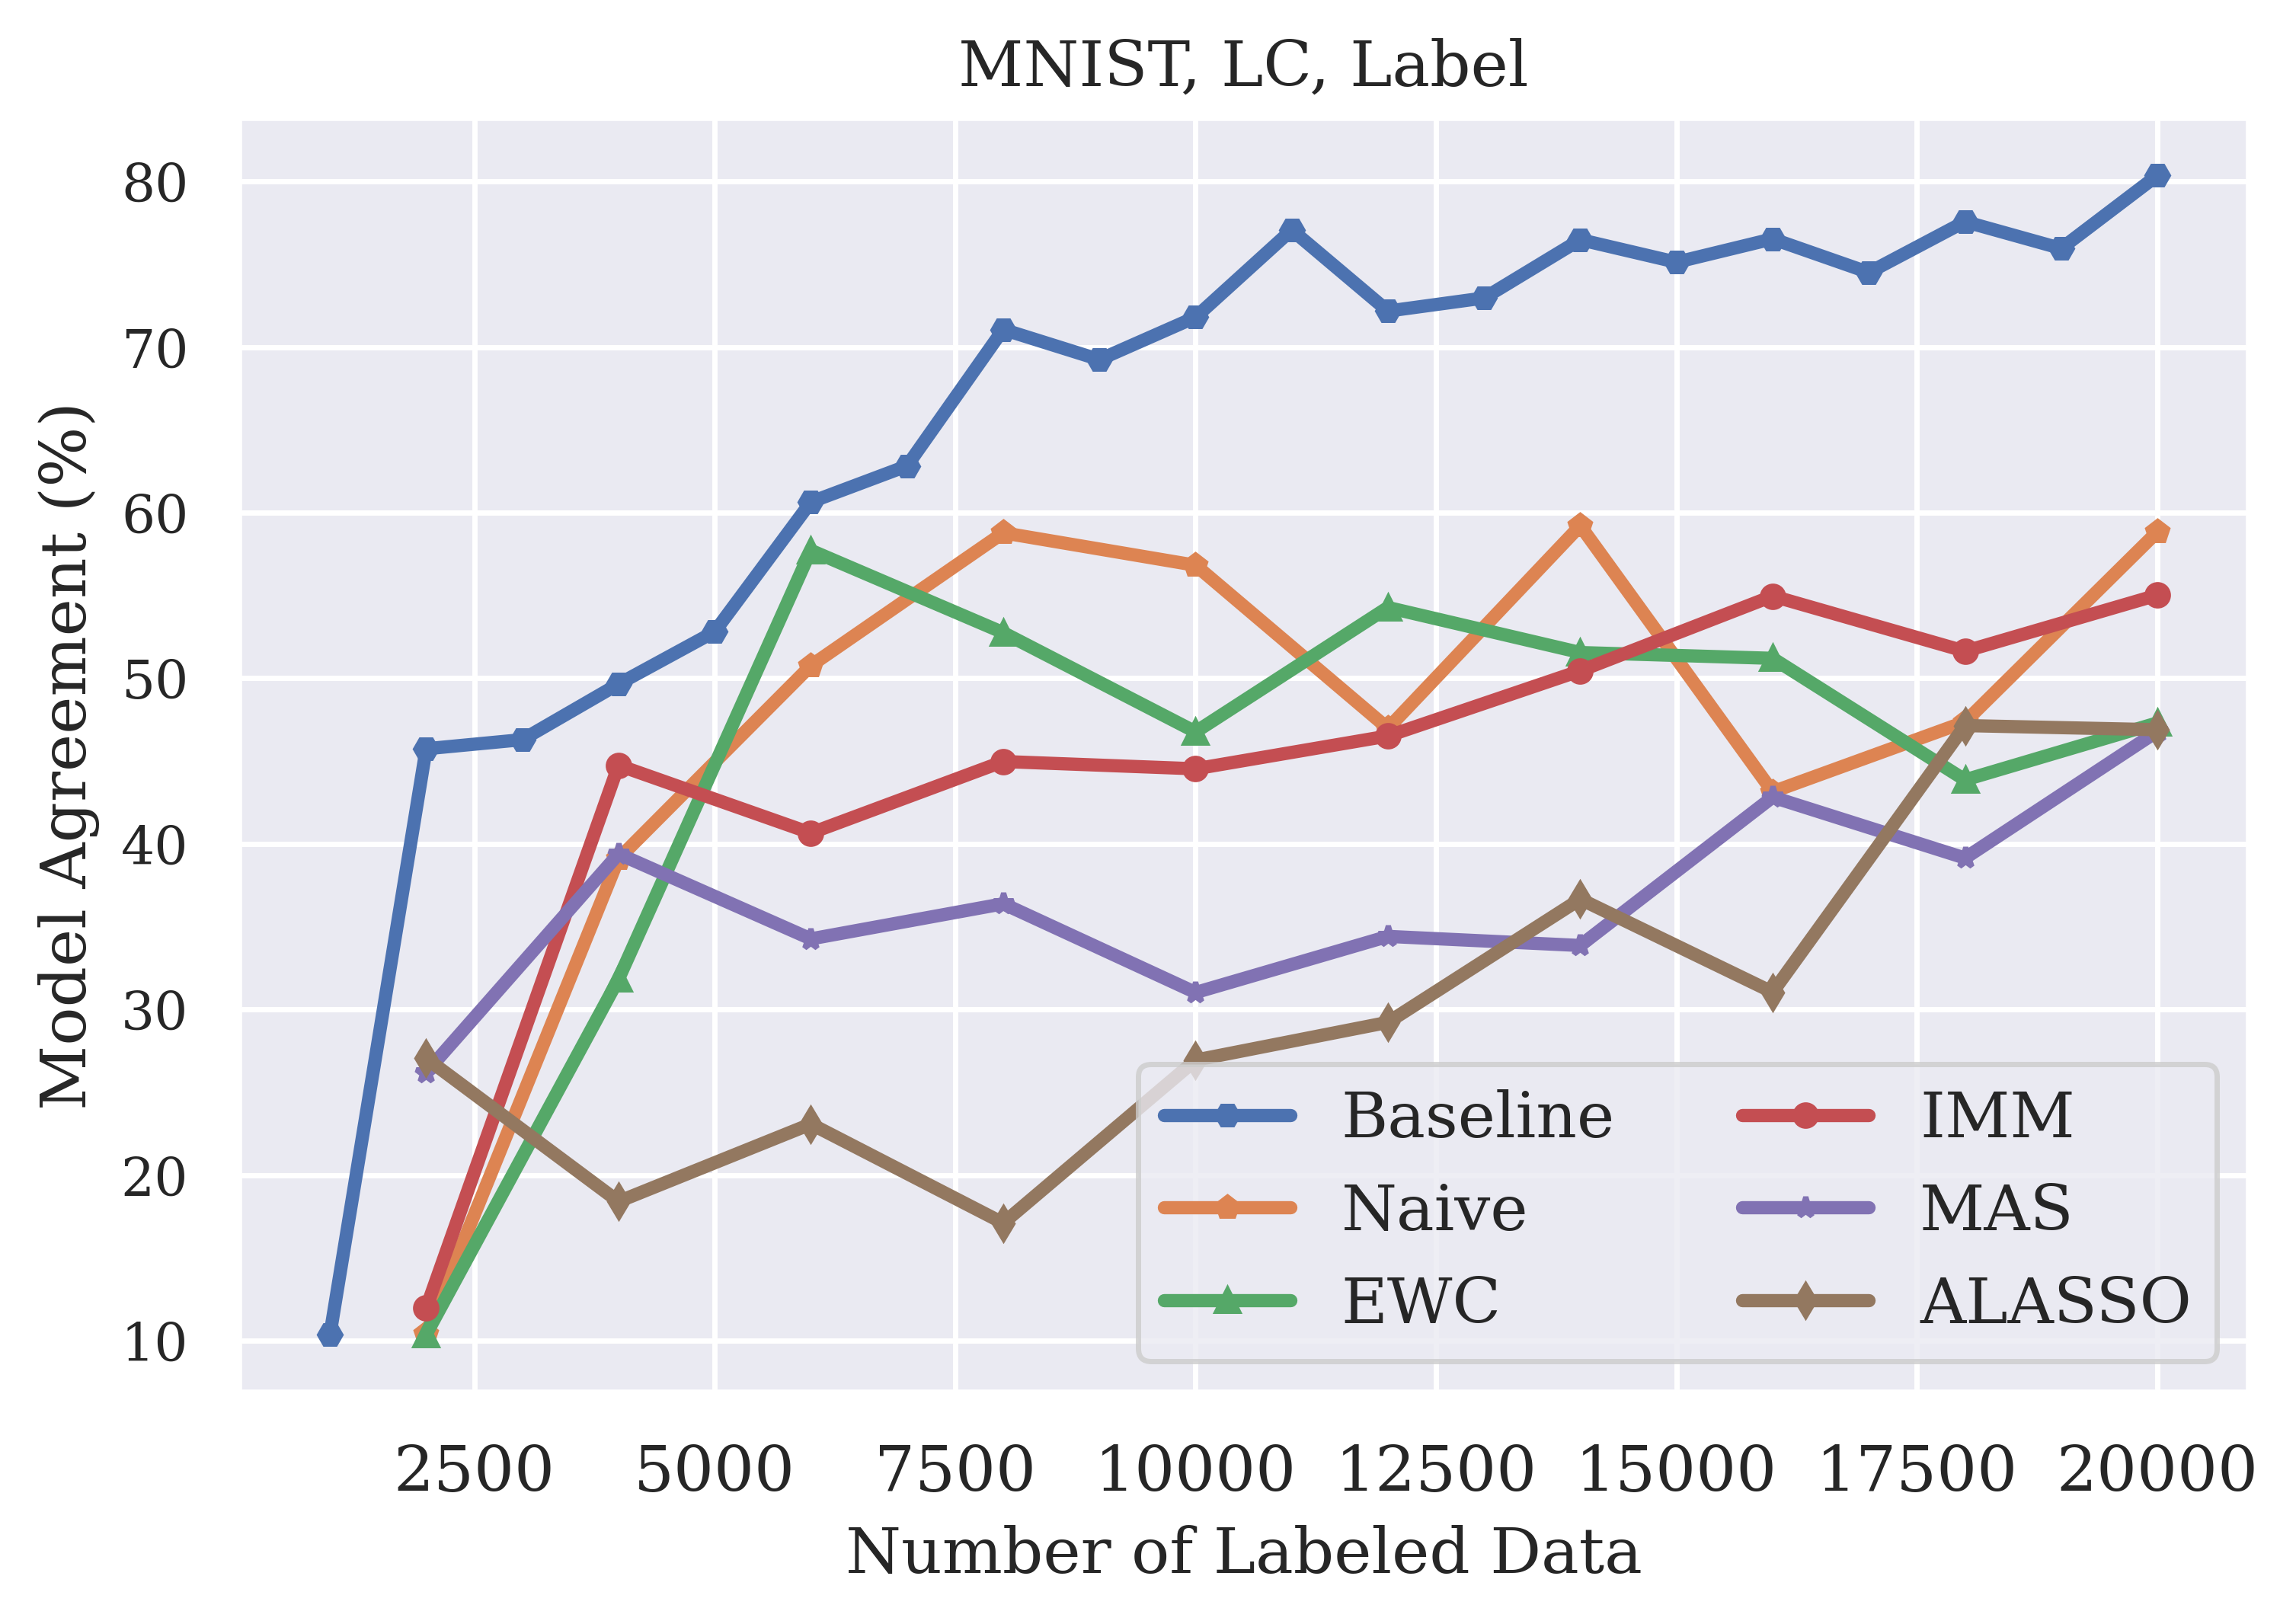
\includegraphics[width=0.48\linewidth]{images/results_CALMS/mnist_label_lc.png} \hfill
    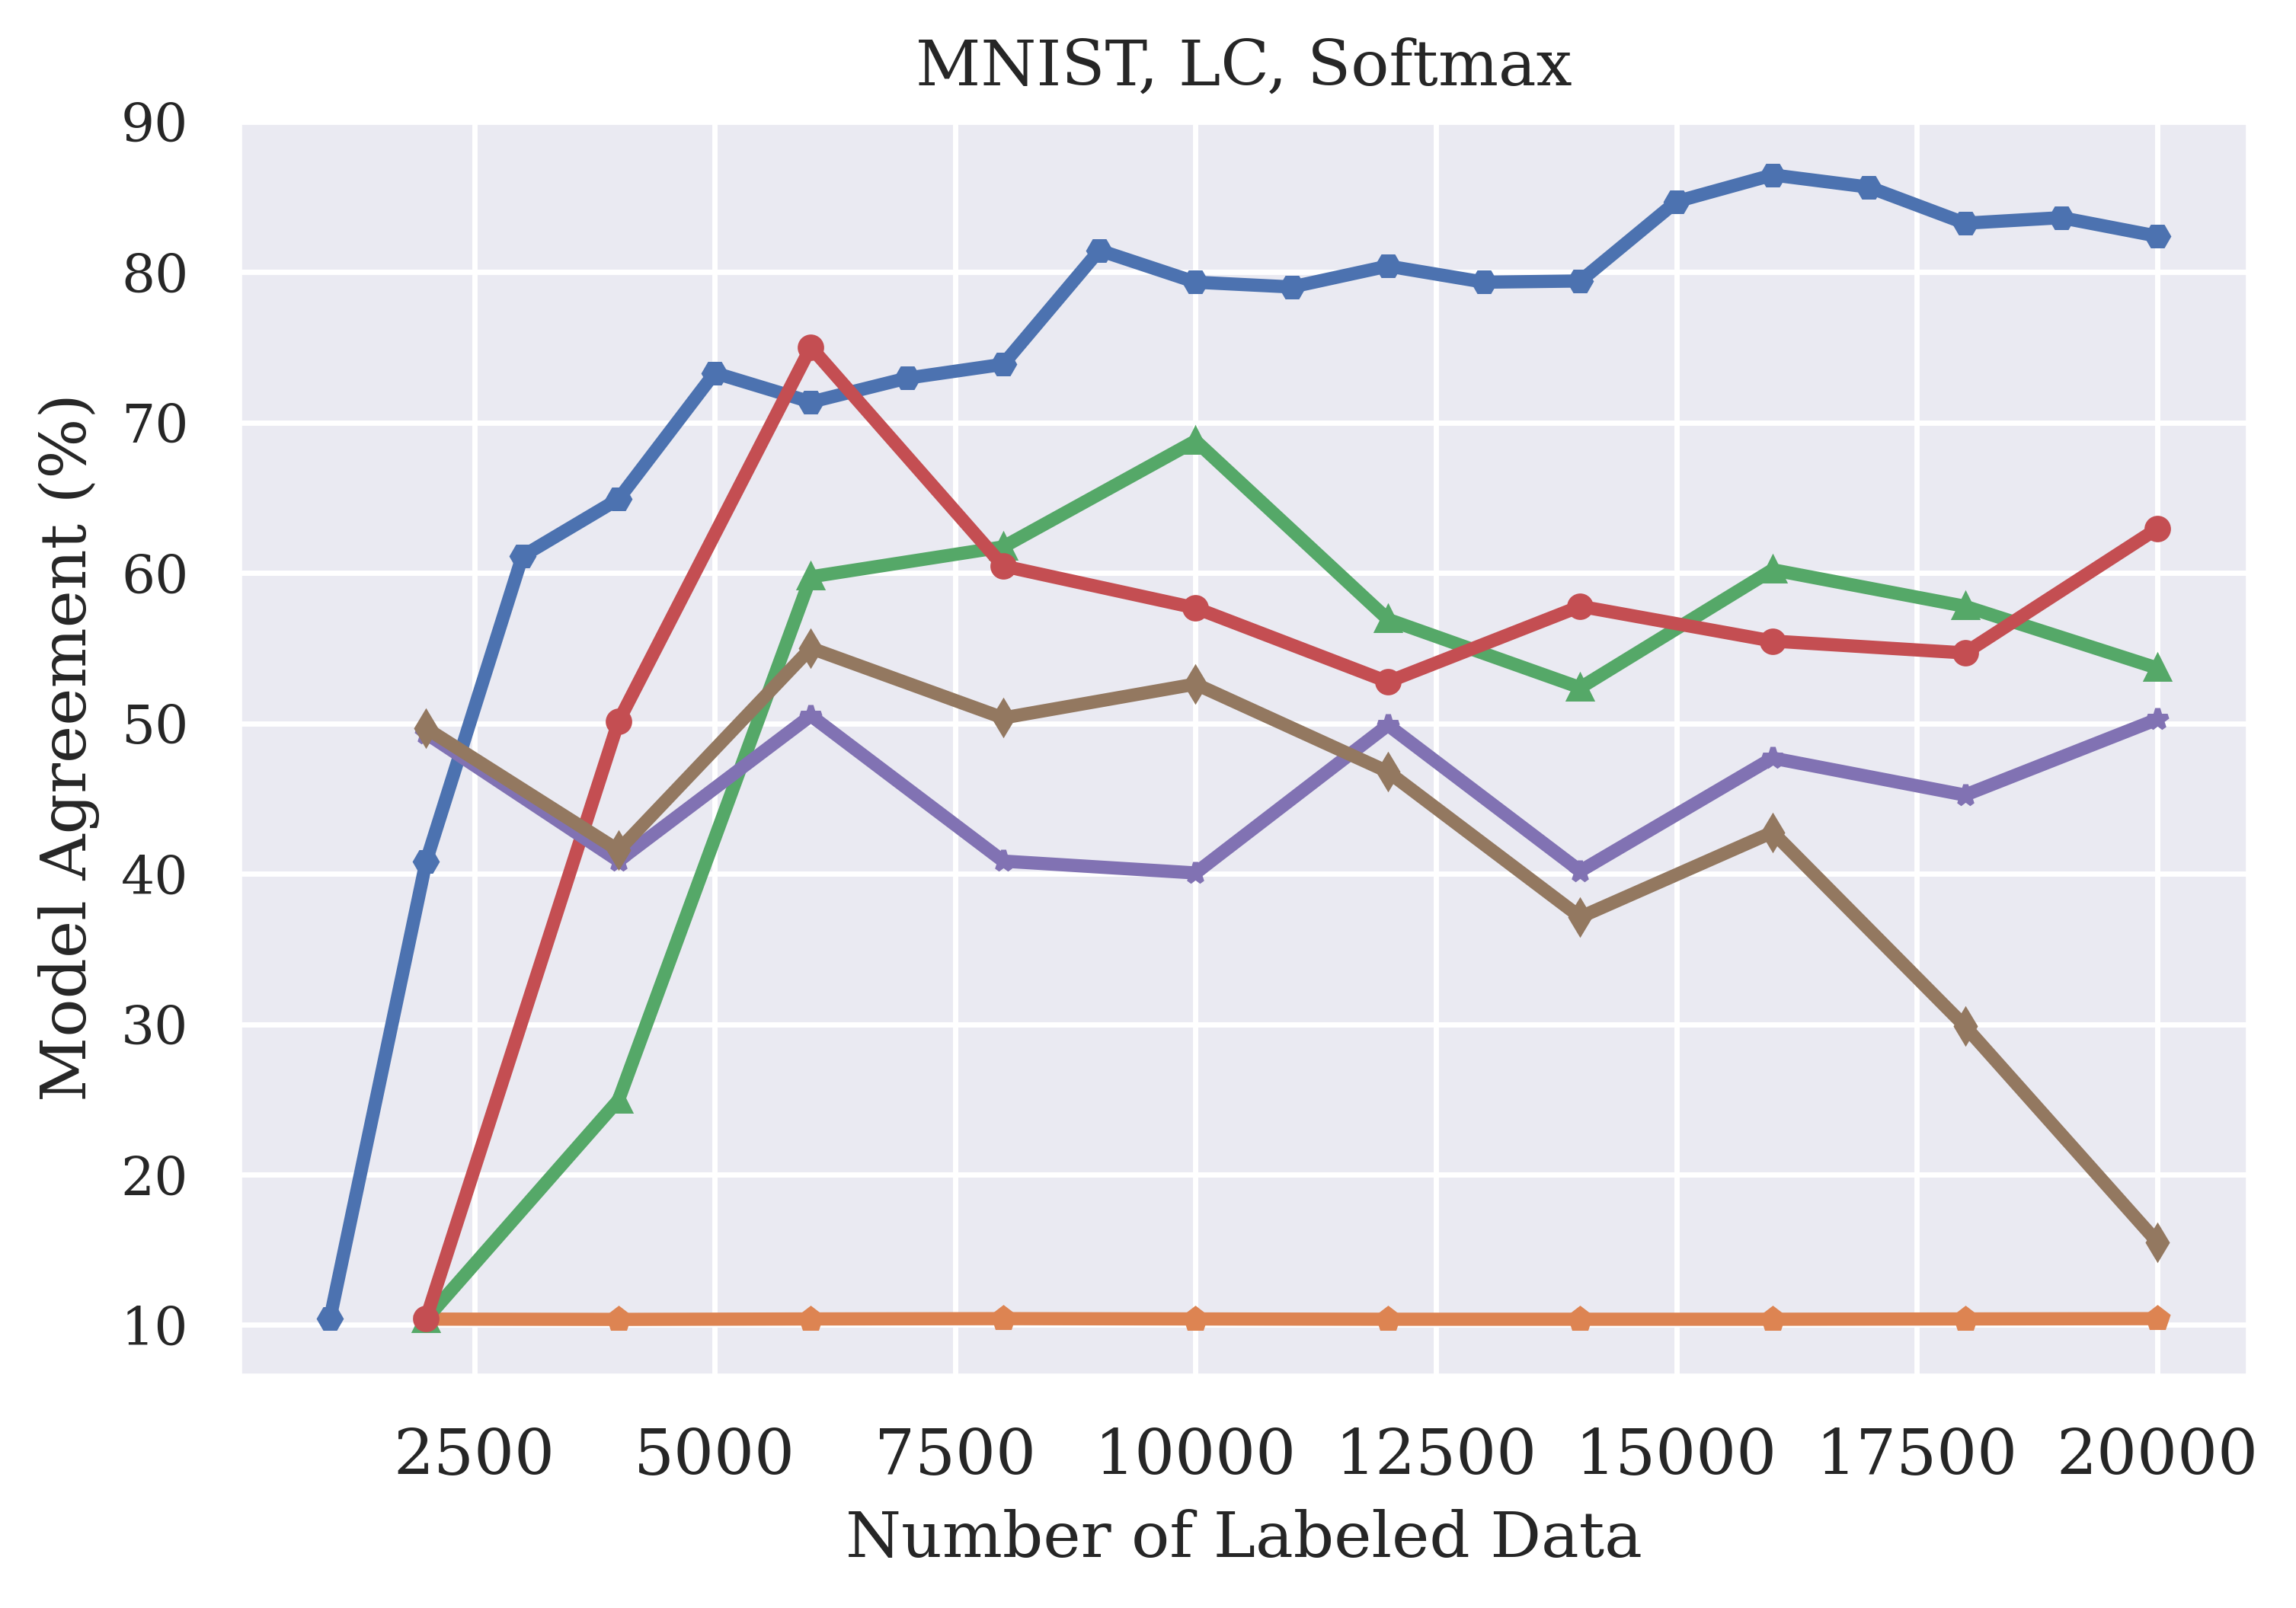
\includegraphics[width=0.48\linewidth]{images/results_CALMS/mnist_softmax_lc.png}
    \caption{Agreement Comparison for Model Stealing on MNIST using the softmax output and the Active Learning strategy \gls{lc}. Left: Training with predicted class label,
    Right: Training with softmax output}
    \label{fig:CALMSMNISTLC}
\end{figure}

\begin{figure}[!htb]
    \centering
    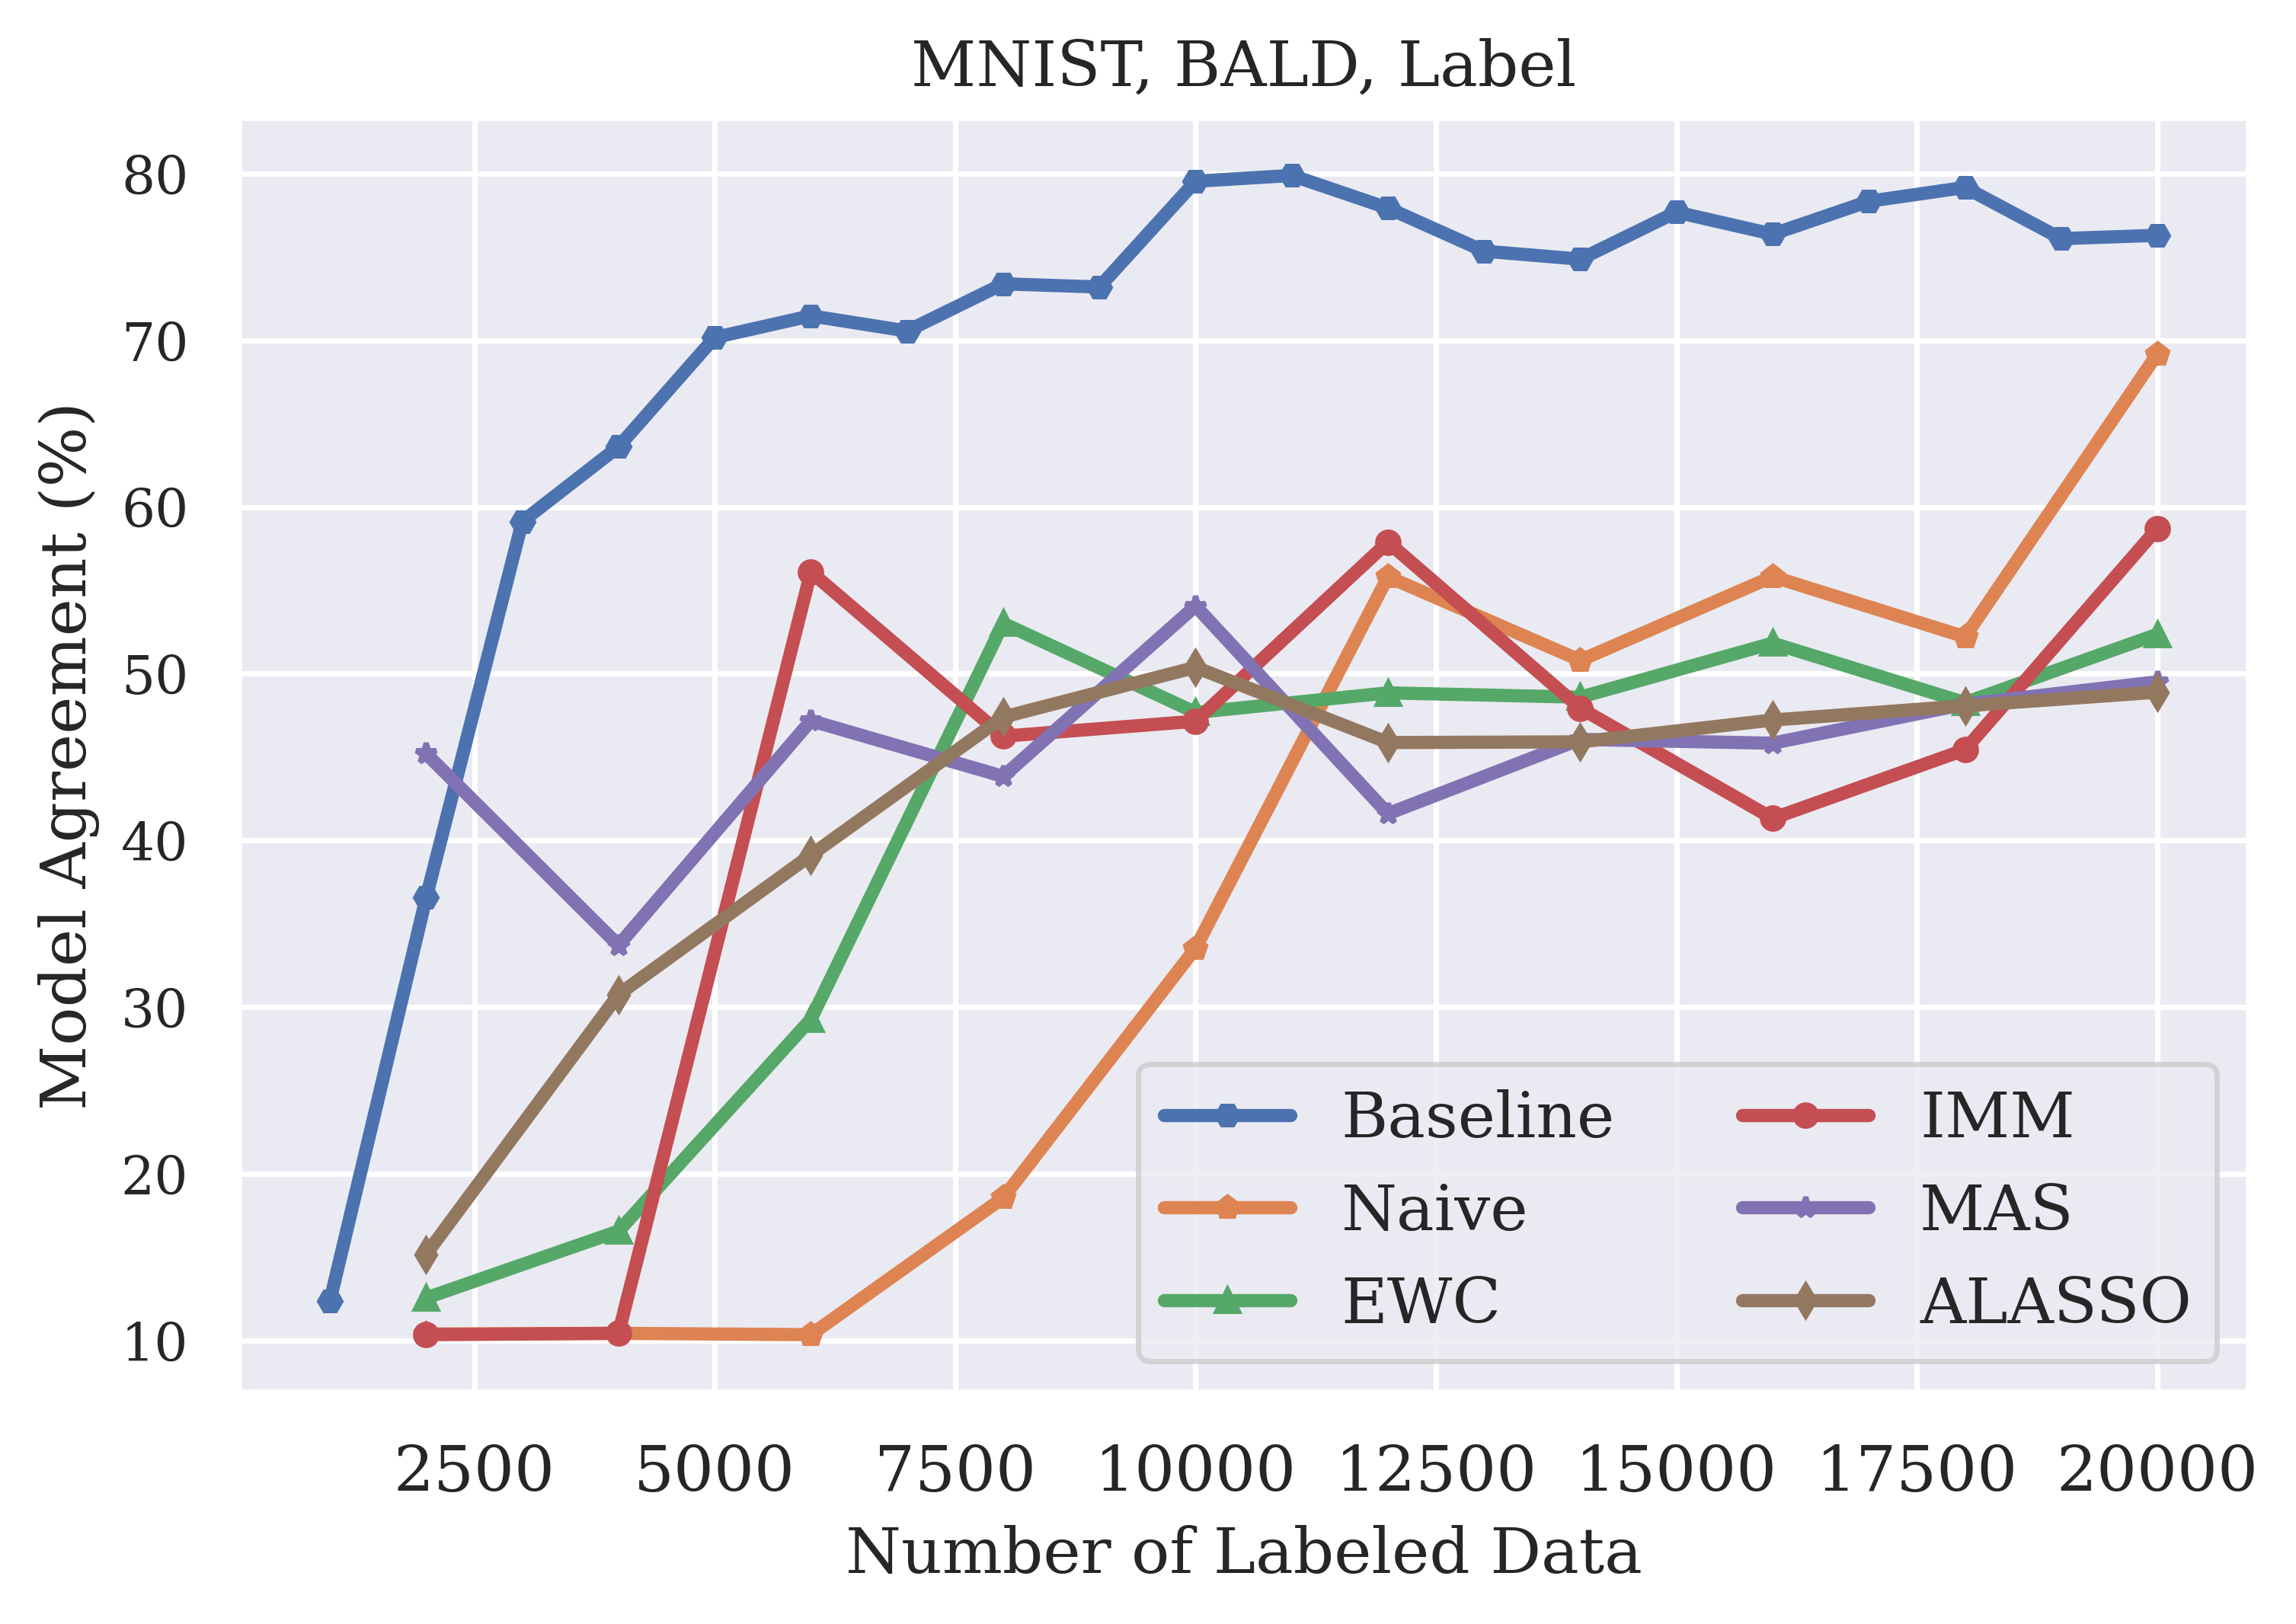
\includegraphics[width=0.48\linewidth]{images/results_CALMS/mnist_label_bald.png} \hfill
    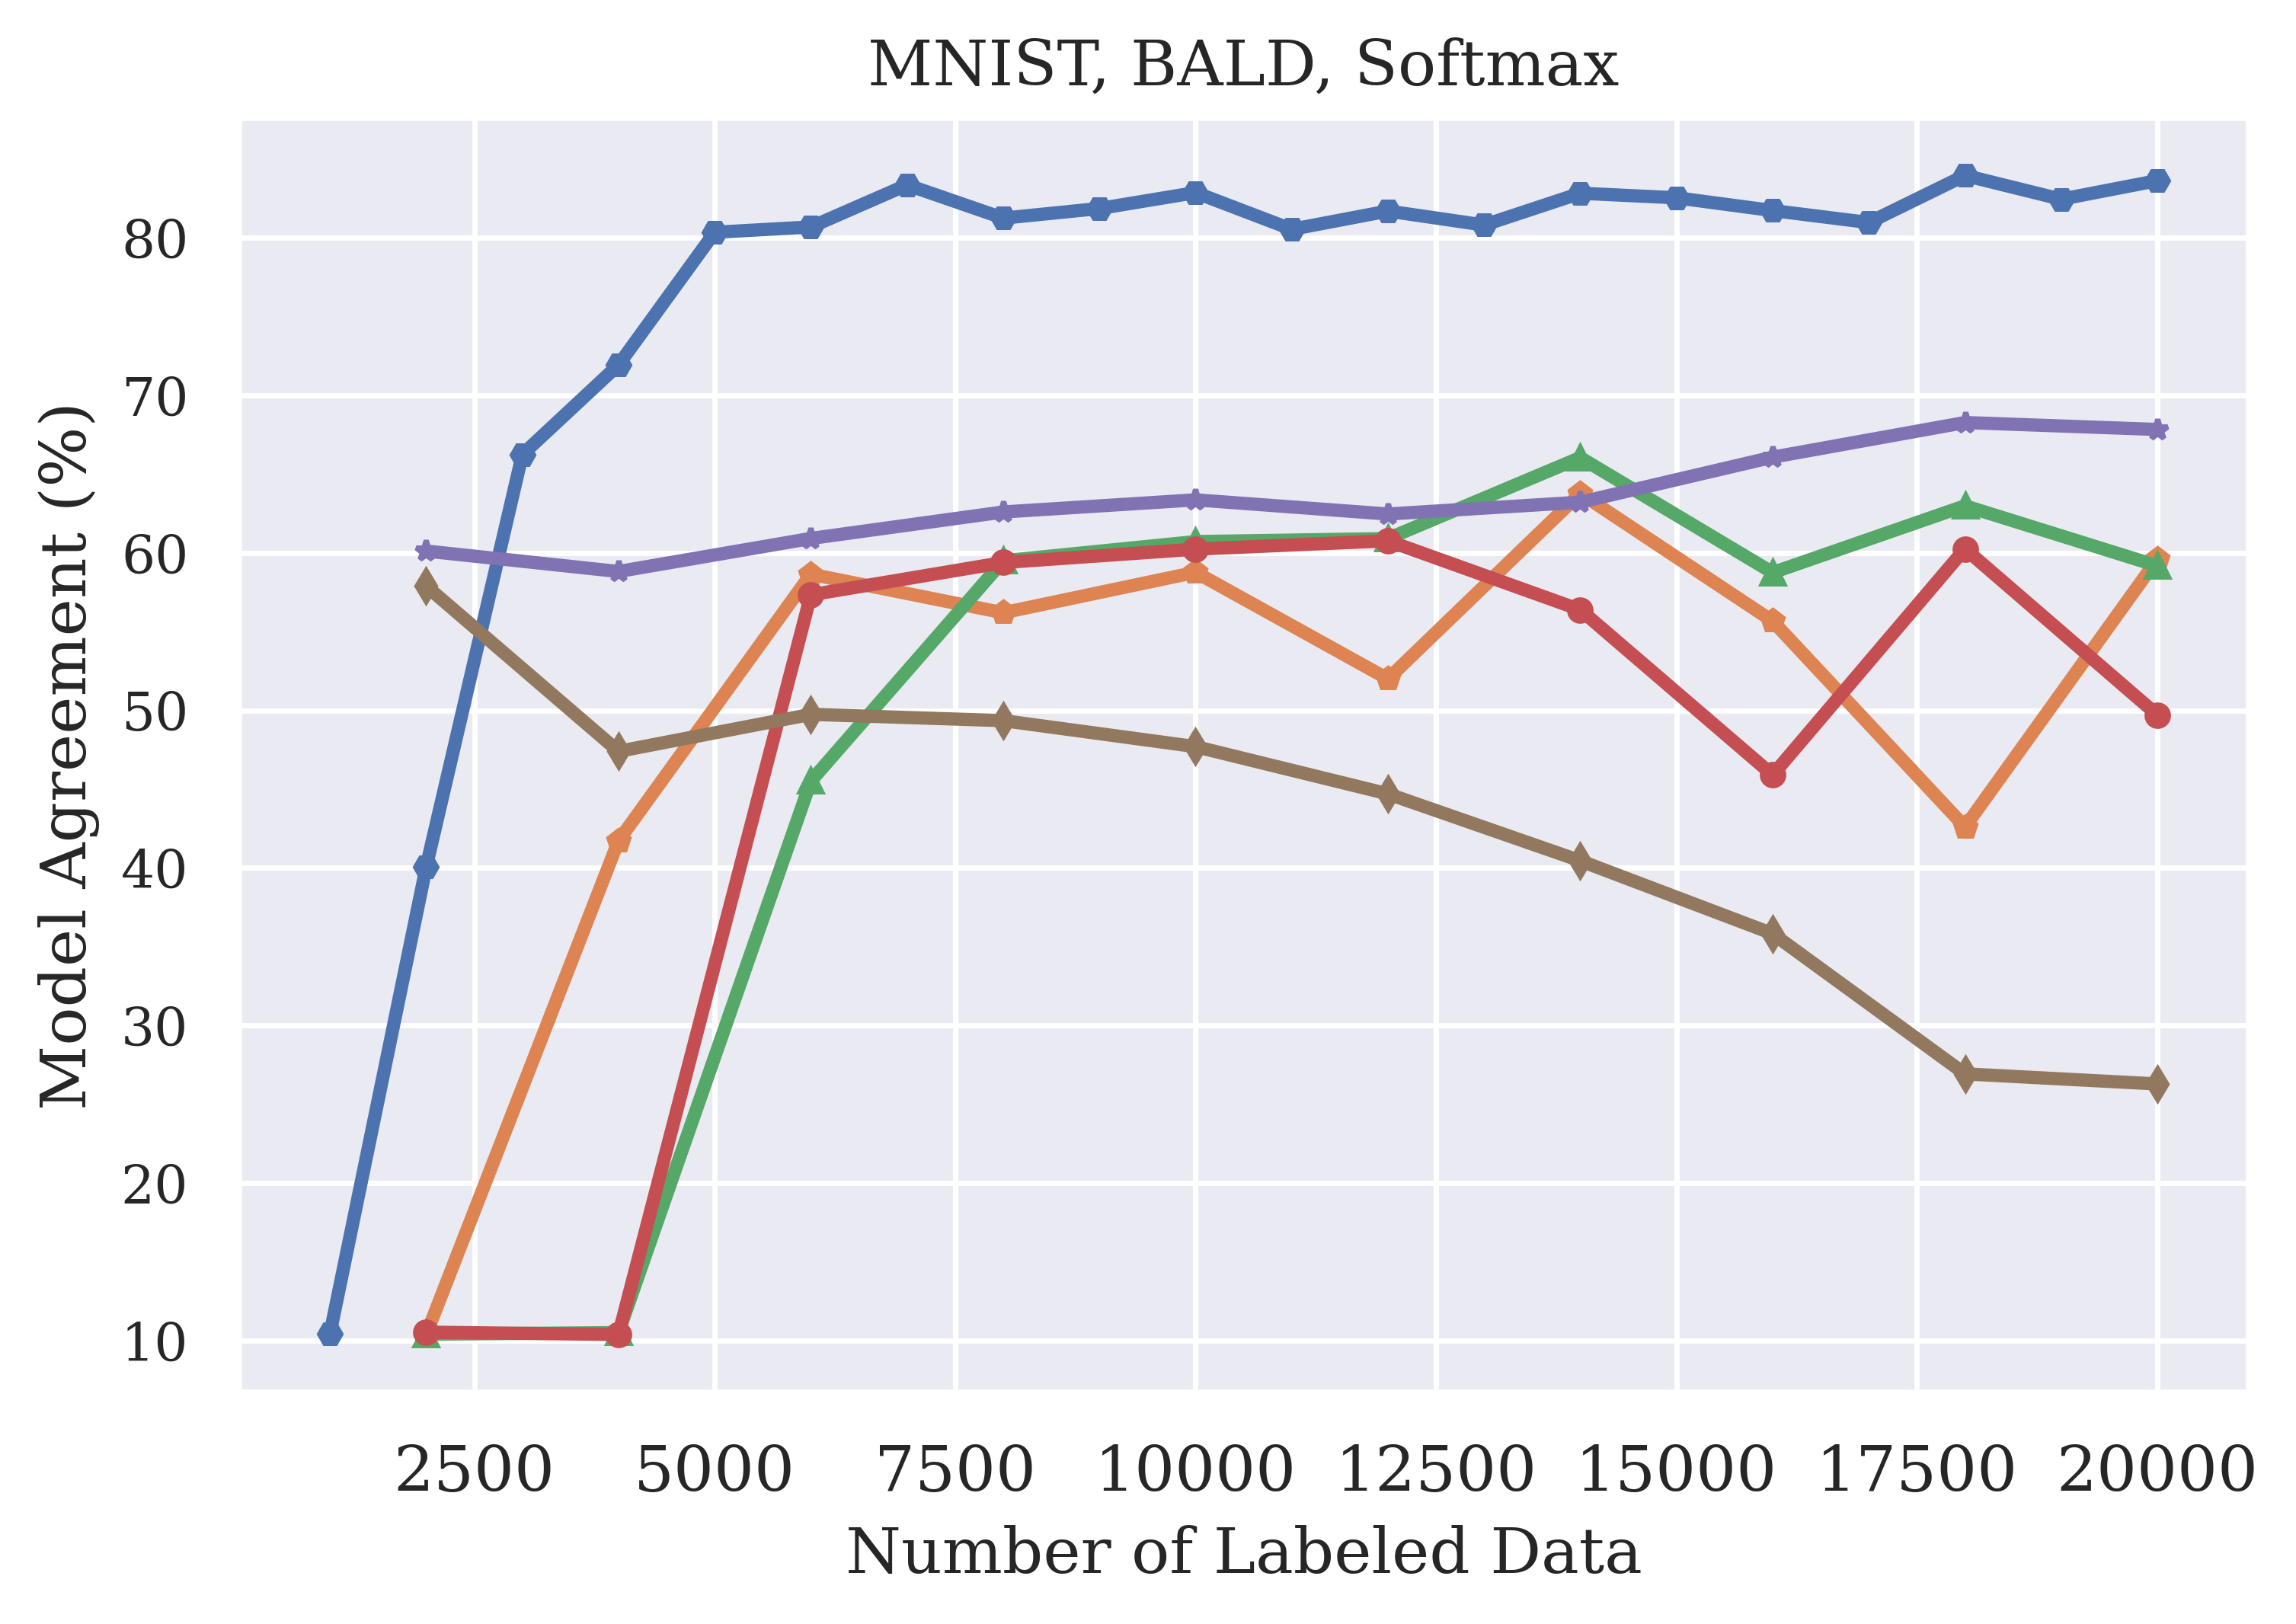
\includegraphics[width=0.48\linewidth]{images/results_CALMS/mnist_softmax_bald.png}
    \caption{Agreement Comparison for Model Stealing on MNIST using the softmax output and the Active Learning strategy \gls{bald}. Left: Training with predicted class label,
    Right: Training with softmax output}
    \label{fig:CALMSMNISTBALD}
\end{figure}

\begin{figure}[!htb]
    \centering
    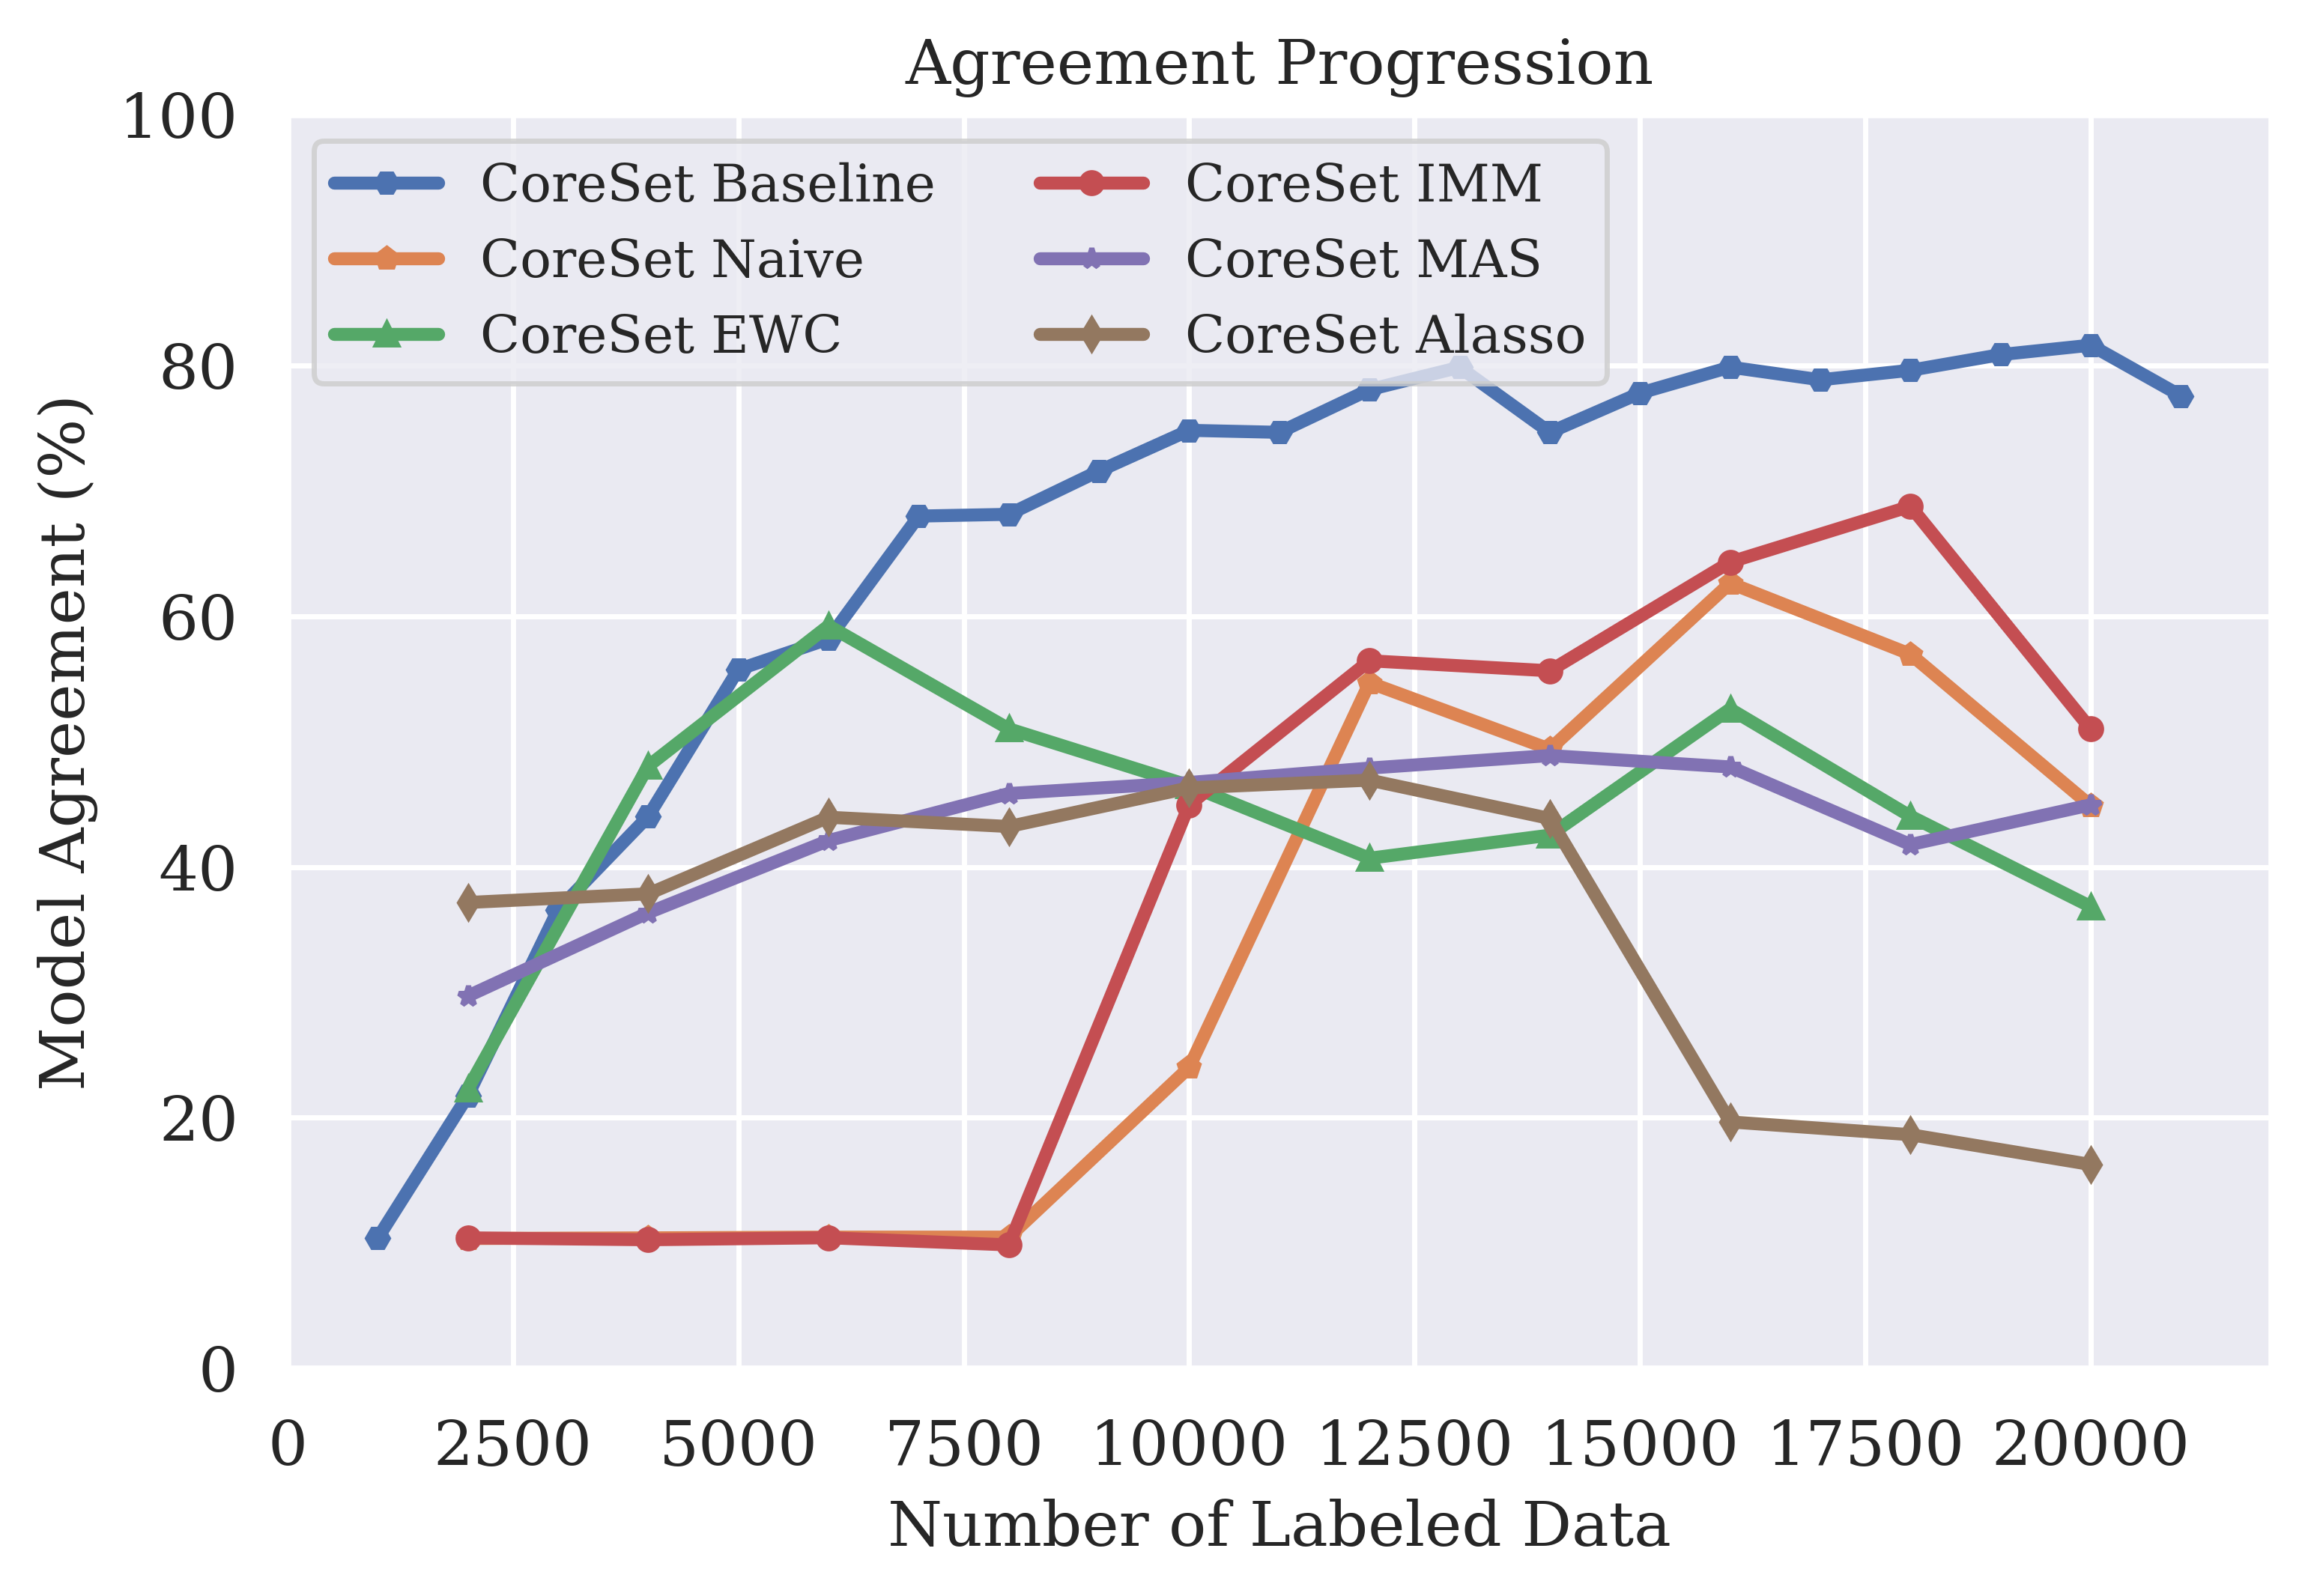
\includegraphics[width=0.48\linewidth]{images/results_CALMS/mnist_label_coreset.png} \hfill
    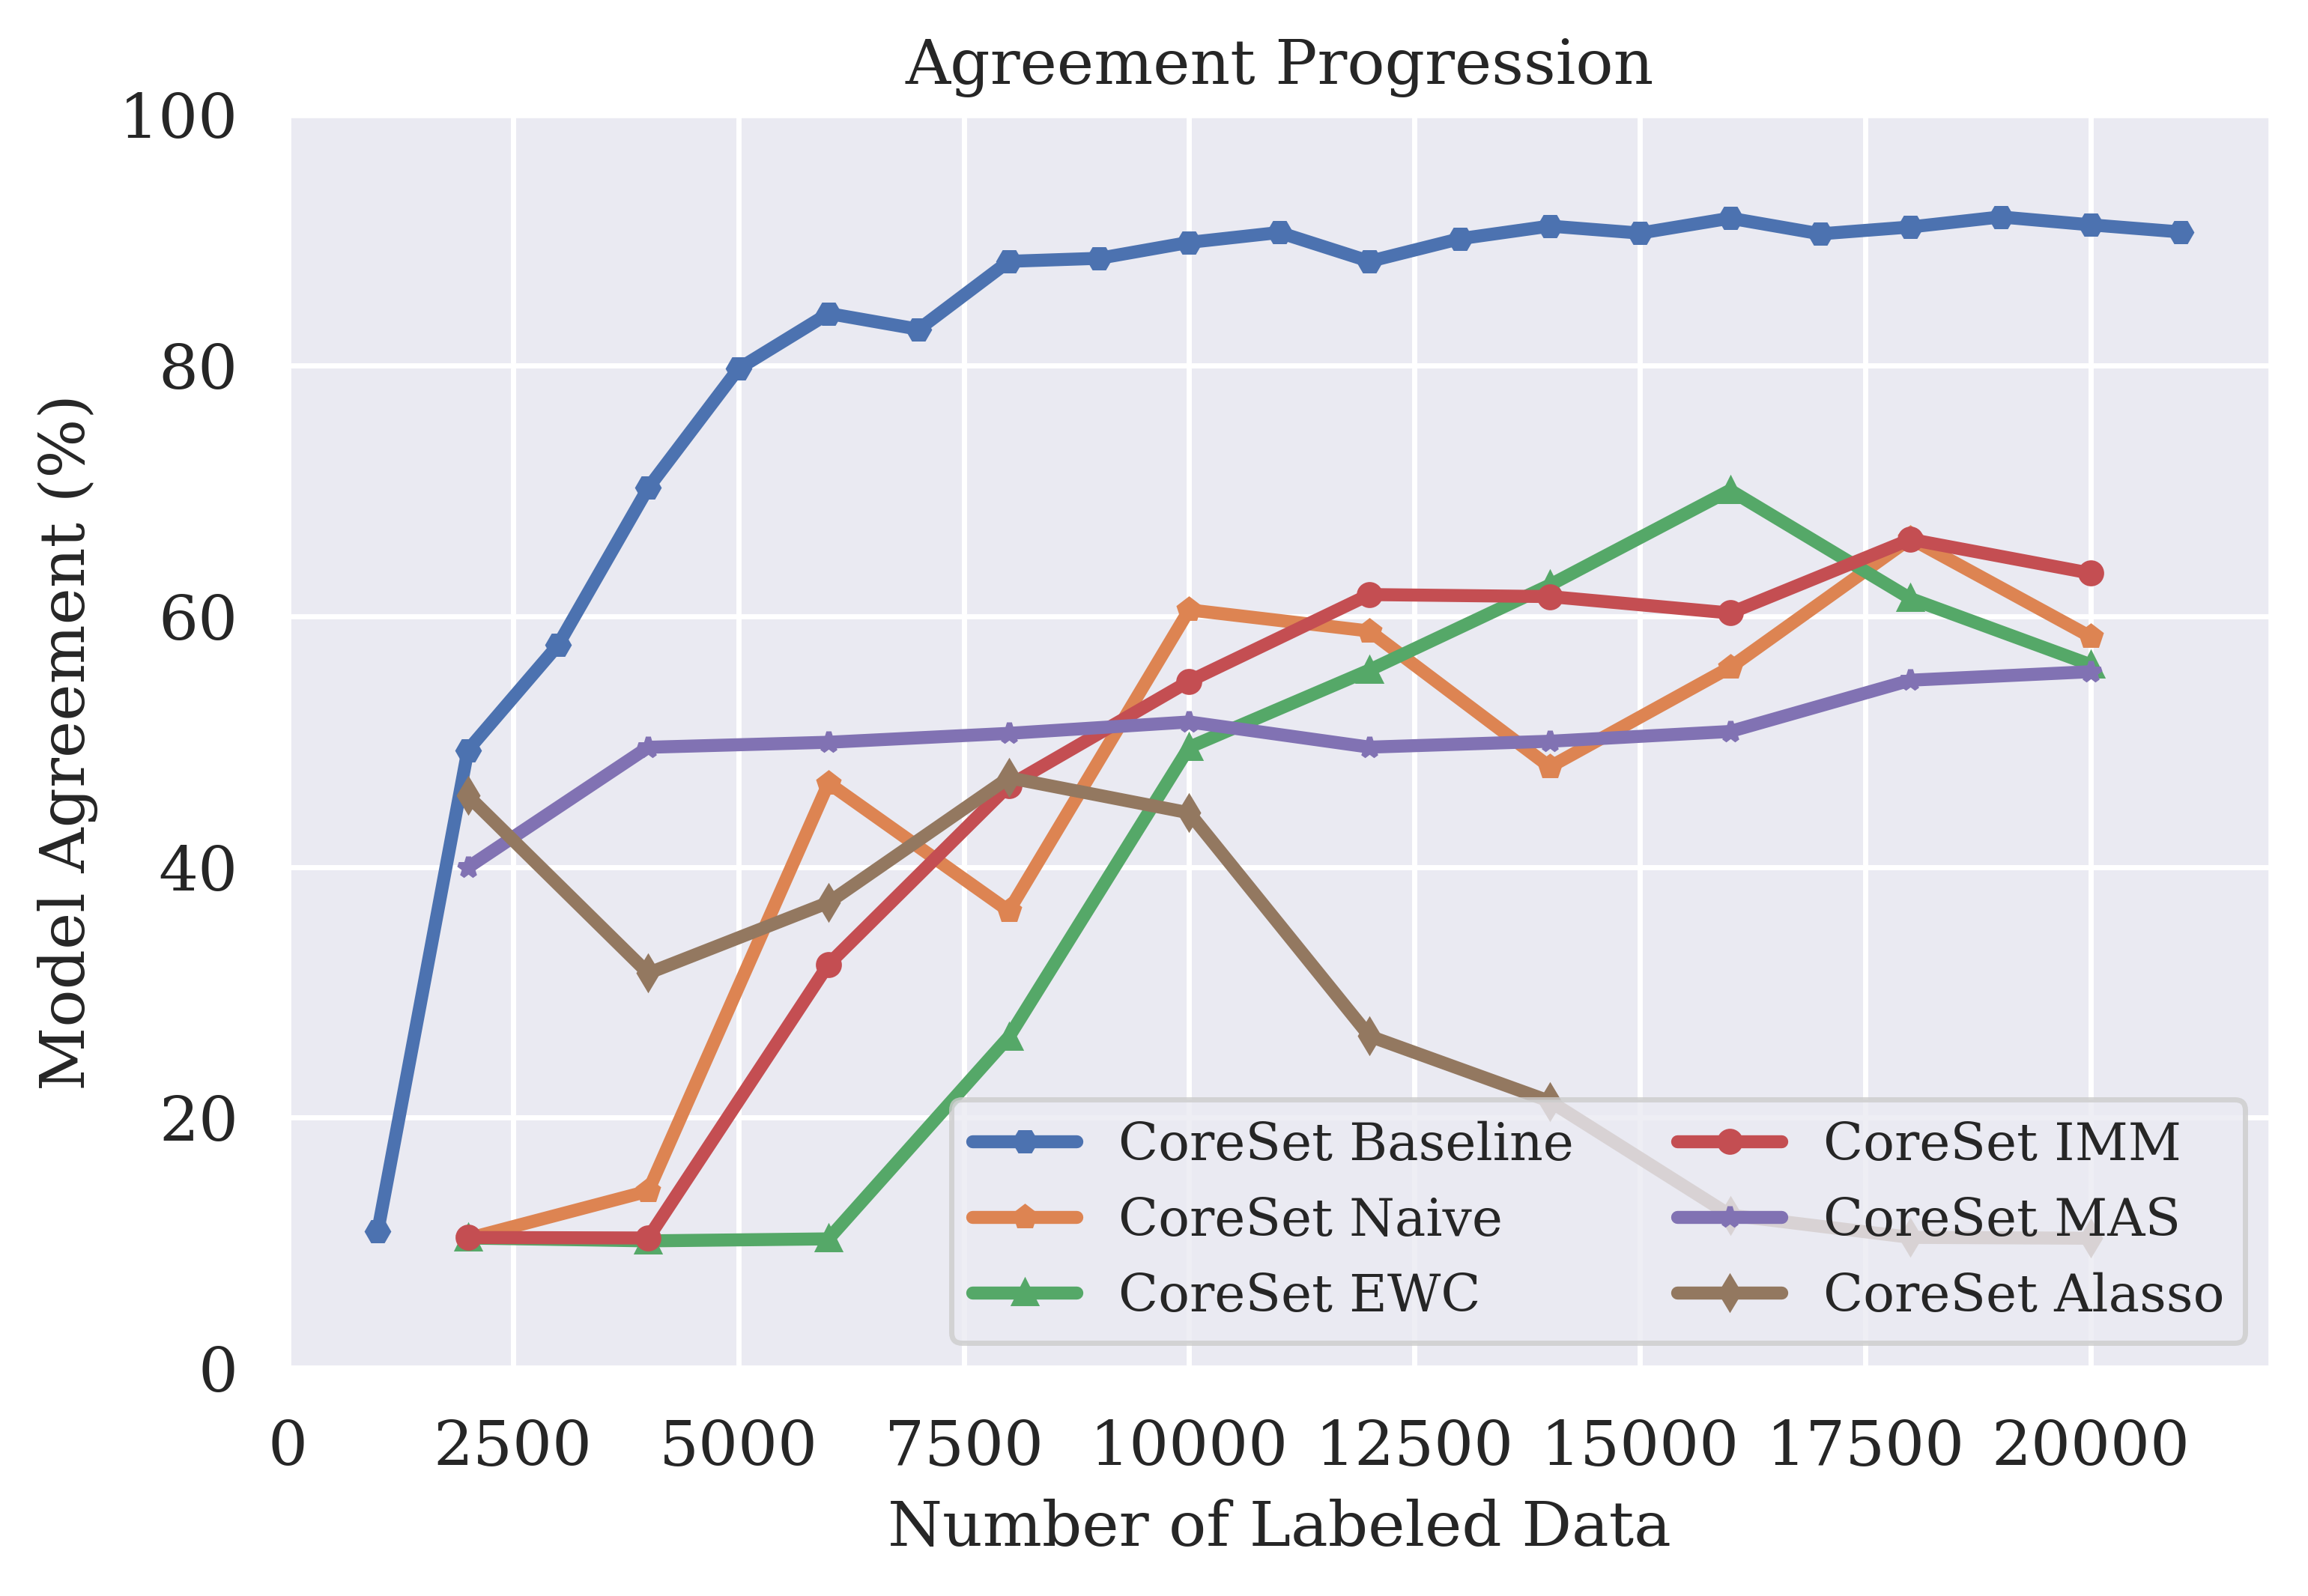
\includegraphics[width=0.48\linewidth]{images/results_CALMS/mnist_softmax_coreset.png}
    \caption{Agreement Comparison for Model Stealing on MNIST using the softmax output and the Active Learning strategy CoreSet. Left: Training with predicted class label,
    Right: Training with softmax output}
    \label{fig:CALMSMNISTCoreSet}
\end{figure}

\begin{figure}[!htb]
    \centering
    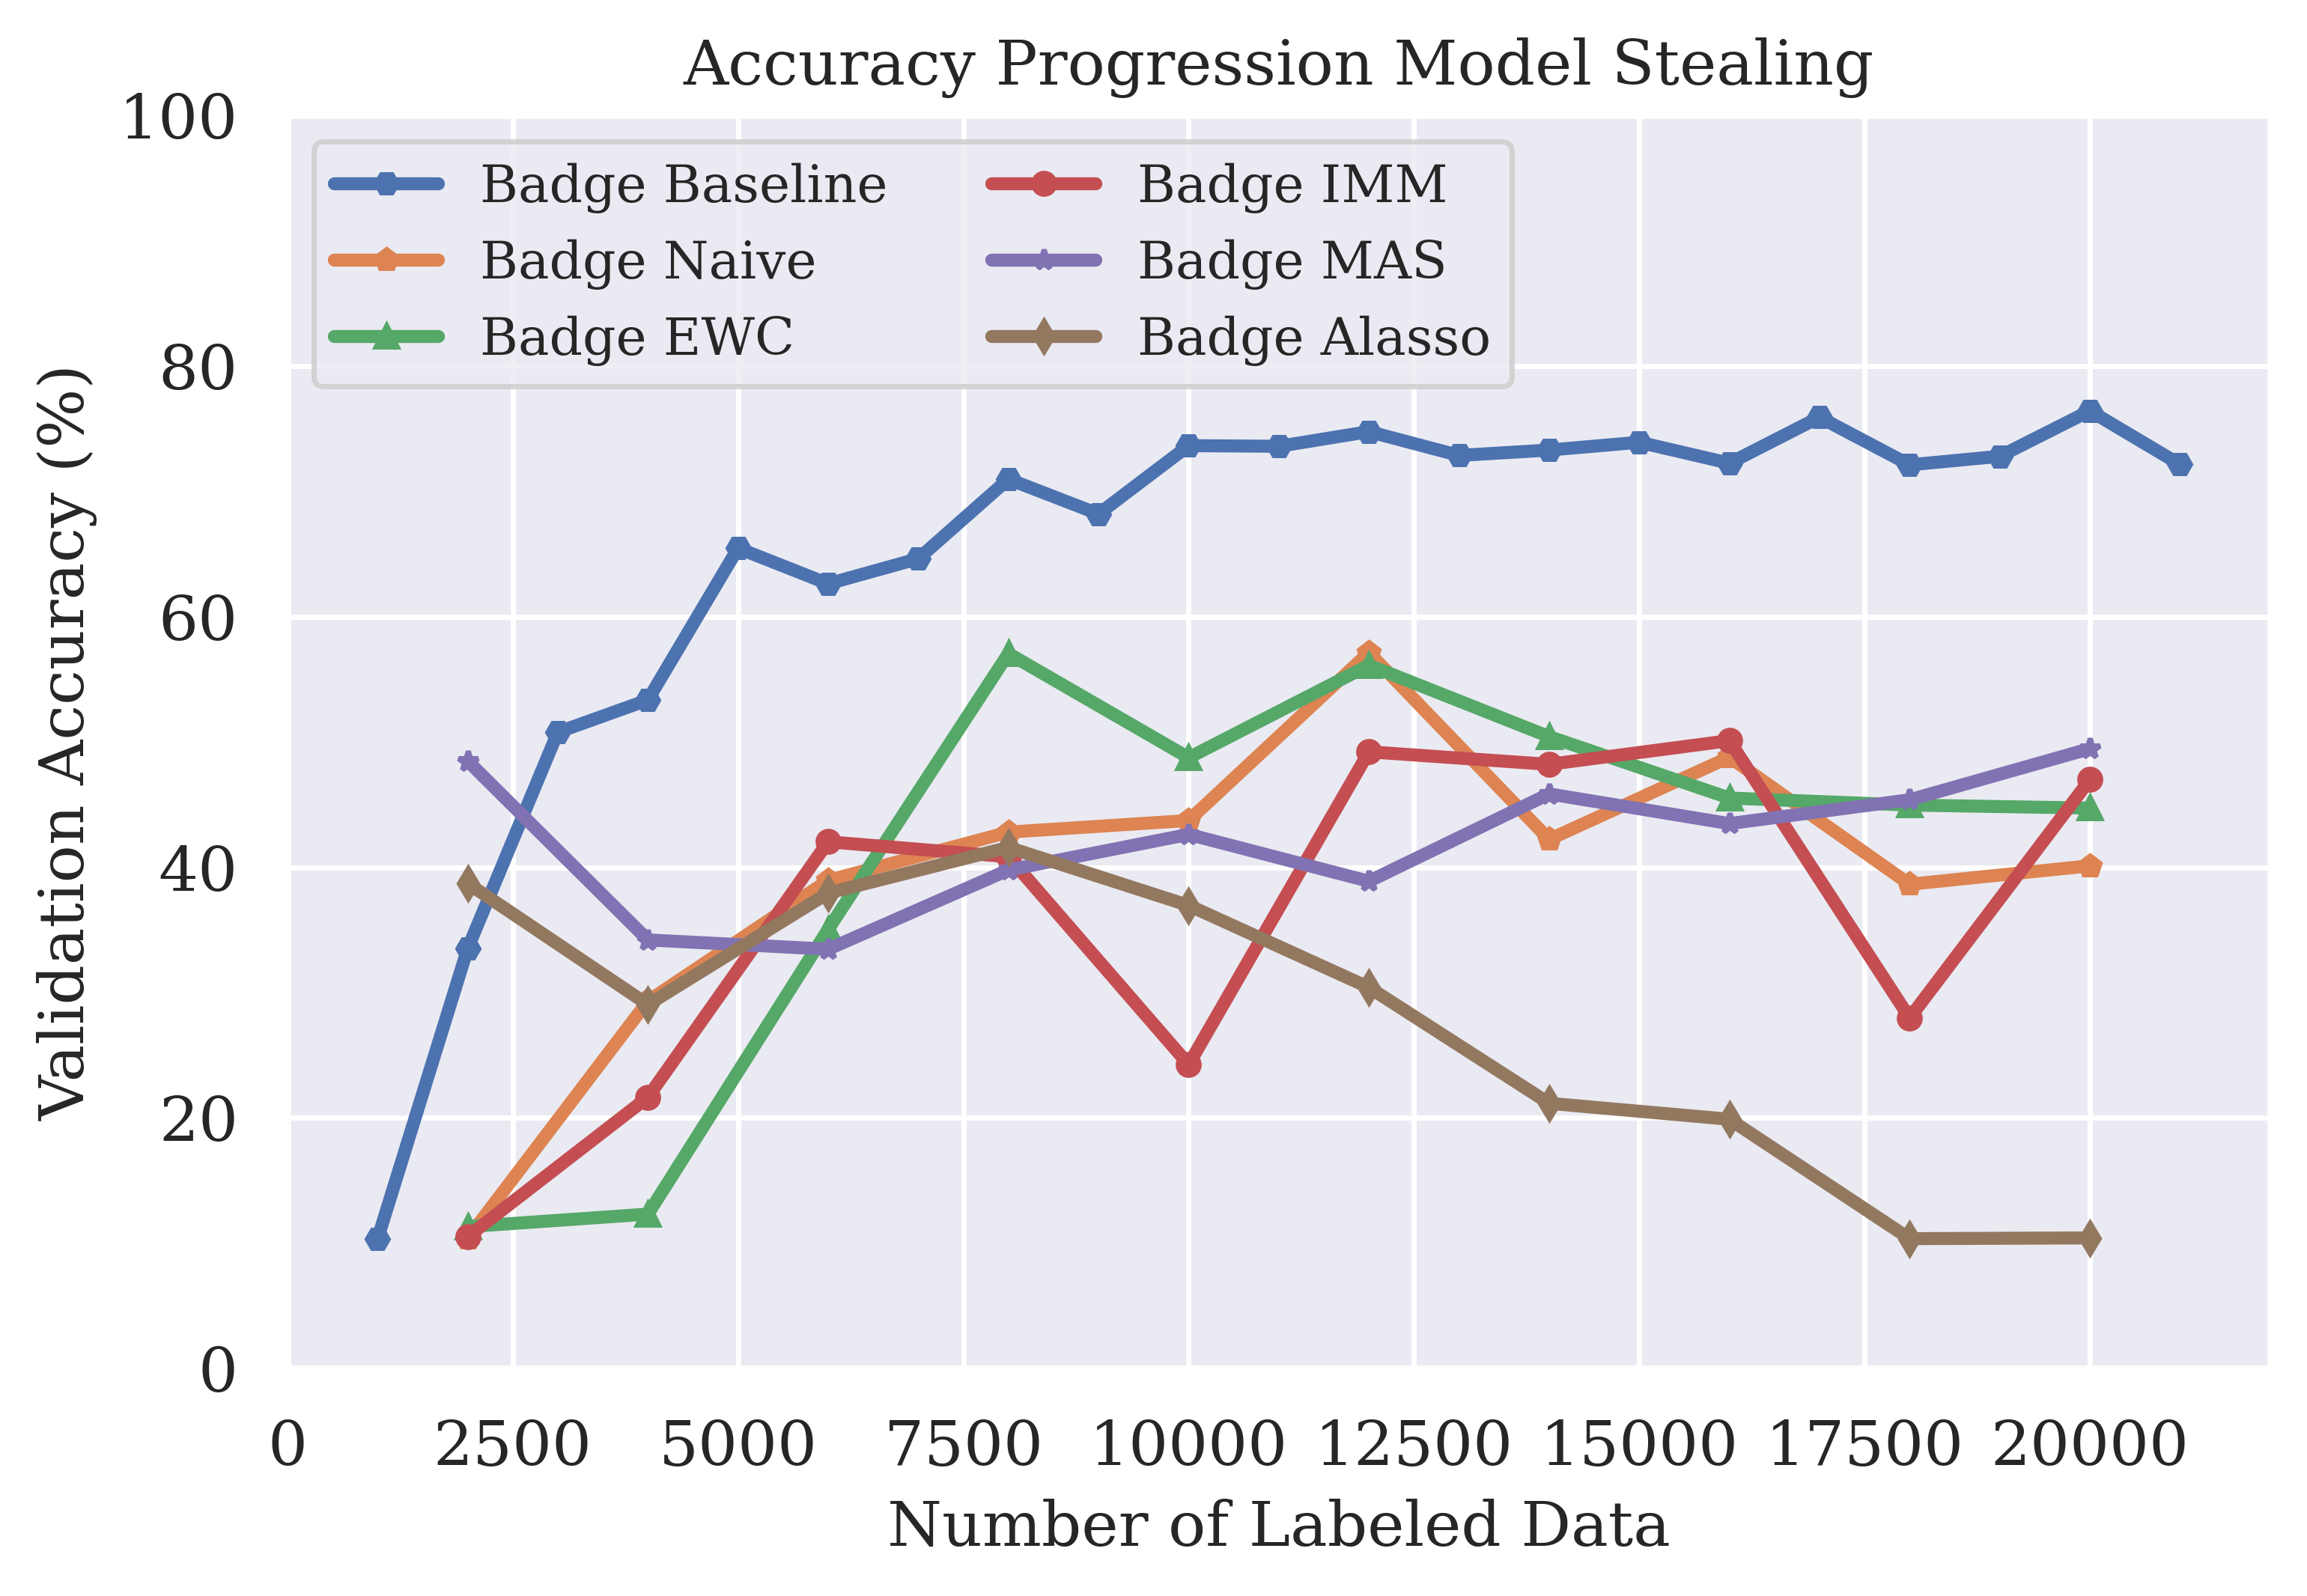
\includegraphics[width=0.48\linewidth]{images/results_CALMS/mnist_label_badge.png} \hfill
    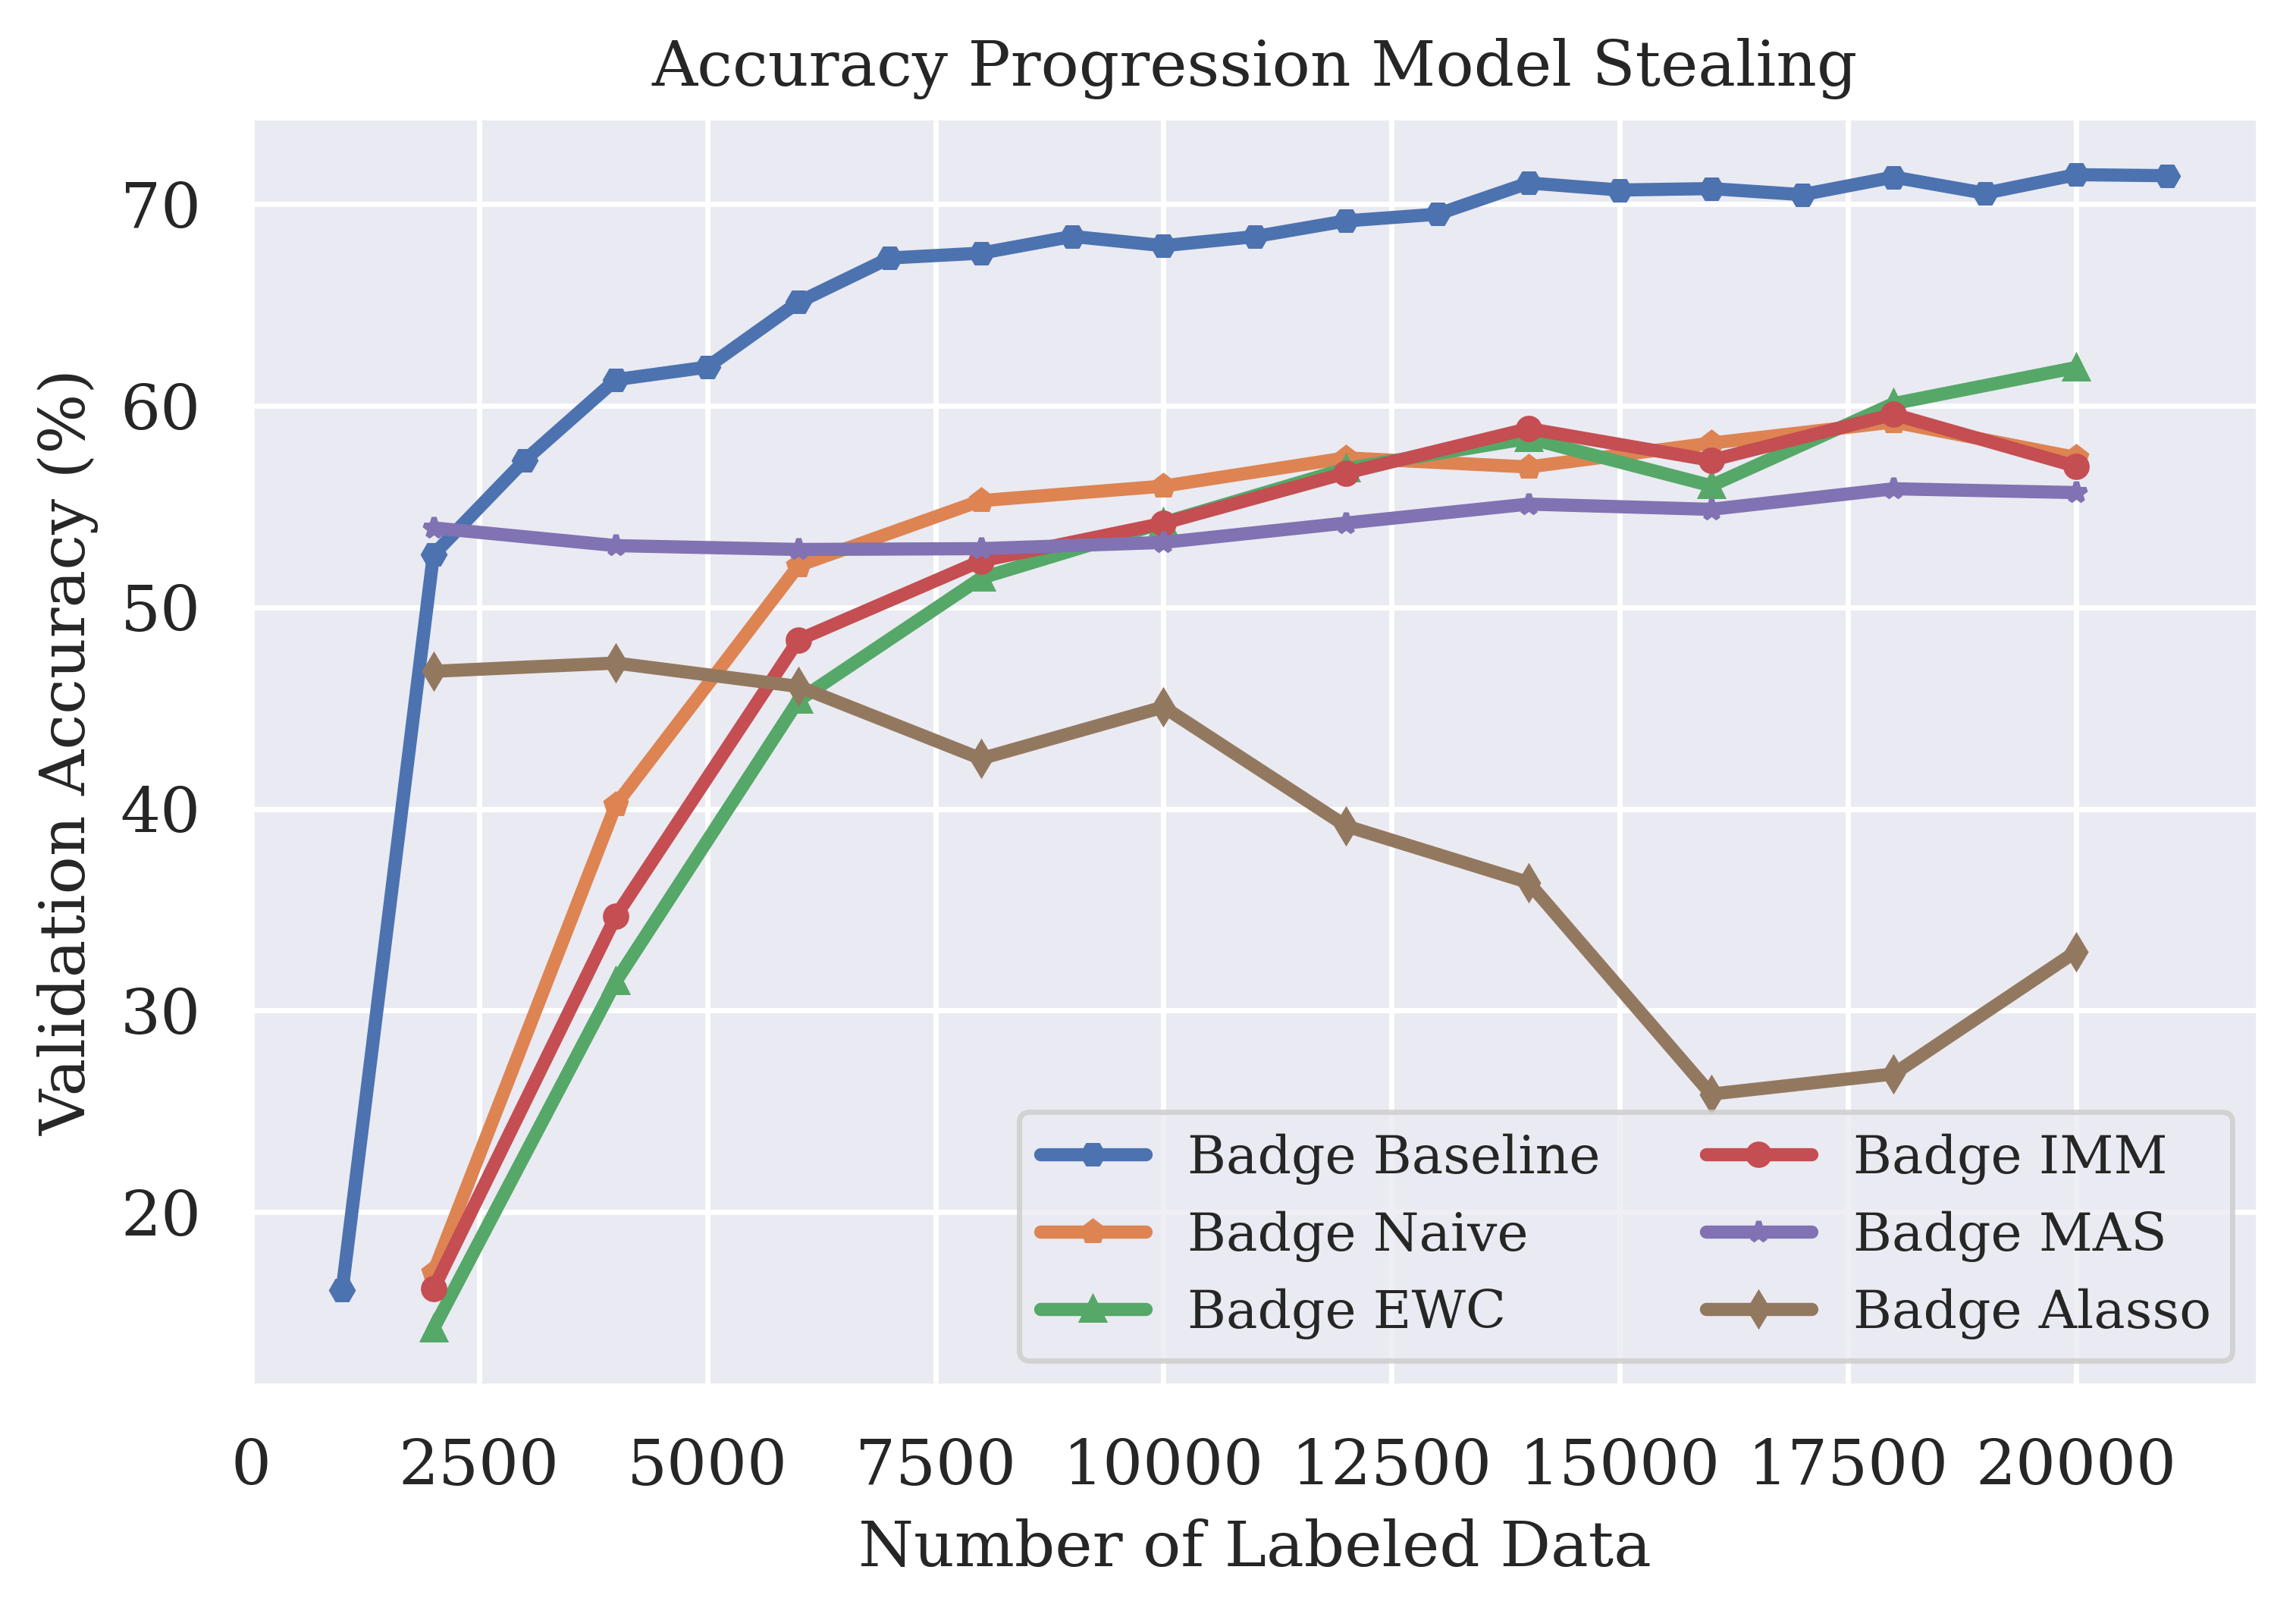
\includegraphics[width=0.48\linewidth]{images/results_CALMS/cifar_softmax_badge.png}
    \caption{Agreement Comparison for Model Stealing on MNIST using the softmax output and the Active Learning strategy \gls{badge}. Left: Training with predicted class label,
    Right: Training with softmax output}
    \label{fig:CALMSMNISTBadge}
\end{figure}

\subsubsection{CIFAR-10}
\label{sec:Appendix:CALMS:CIFAR}
In this section, we present the full runs of all experiments which involve Continual Active Learning using CIFAR-10 as a Target Model Dataset.

\begin{figure}[!htb]
    \centering
    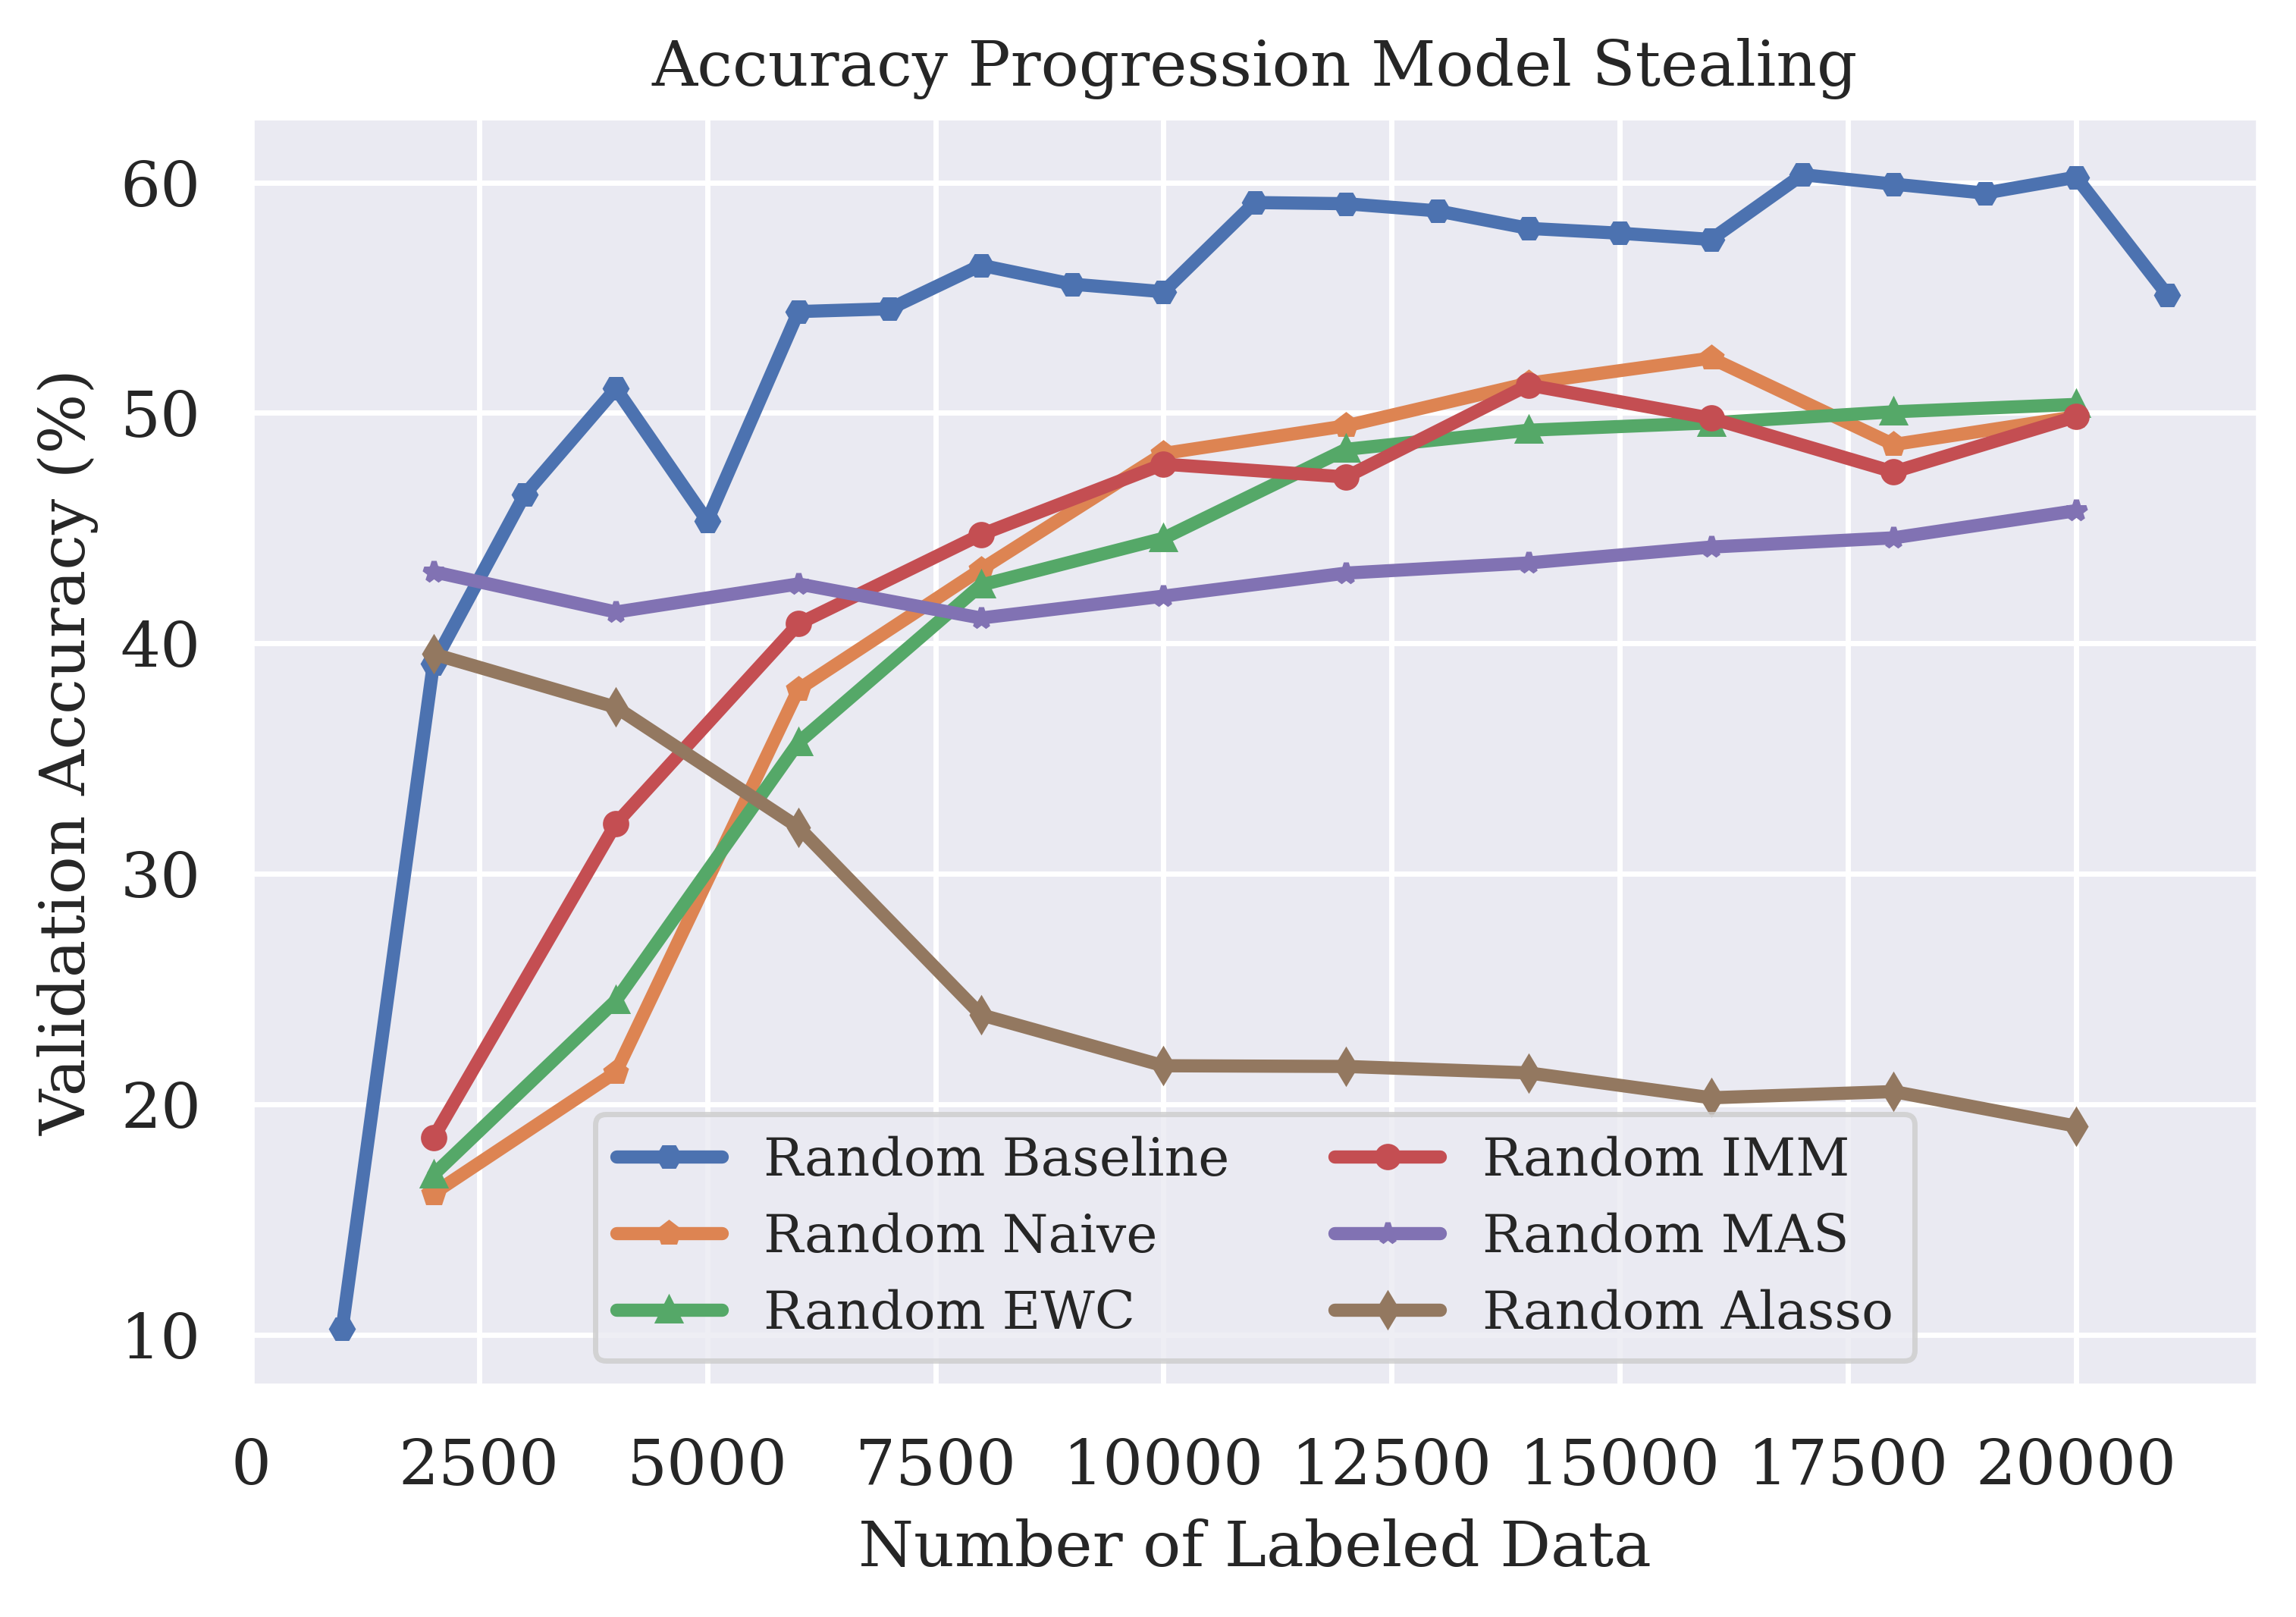
\includegraphics[width=0.48\linewidth]{images/results_CALMS/cifar_label_random.png} \hfill
    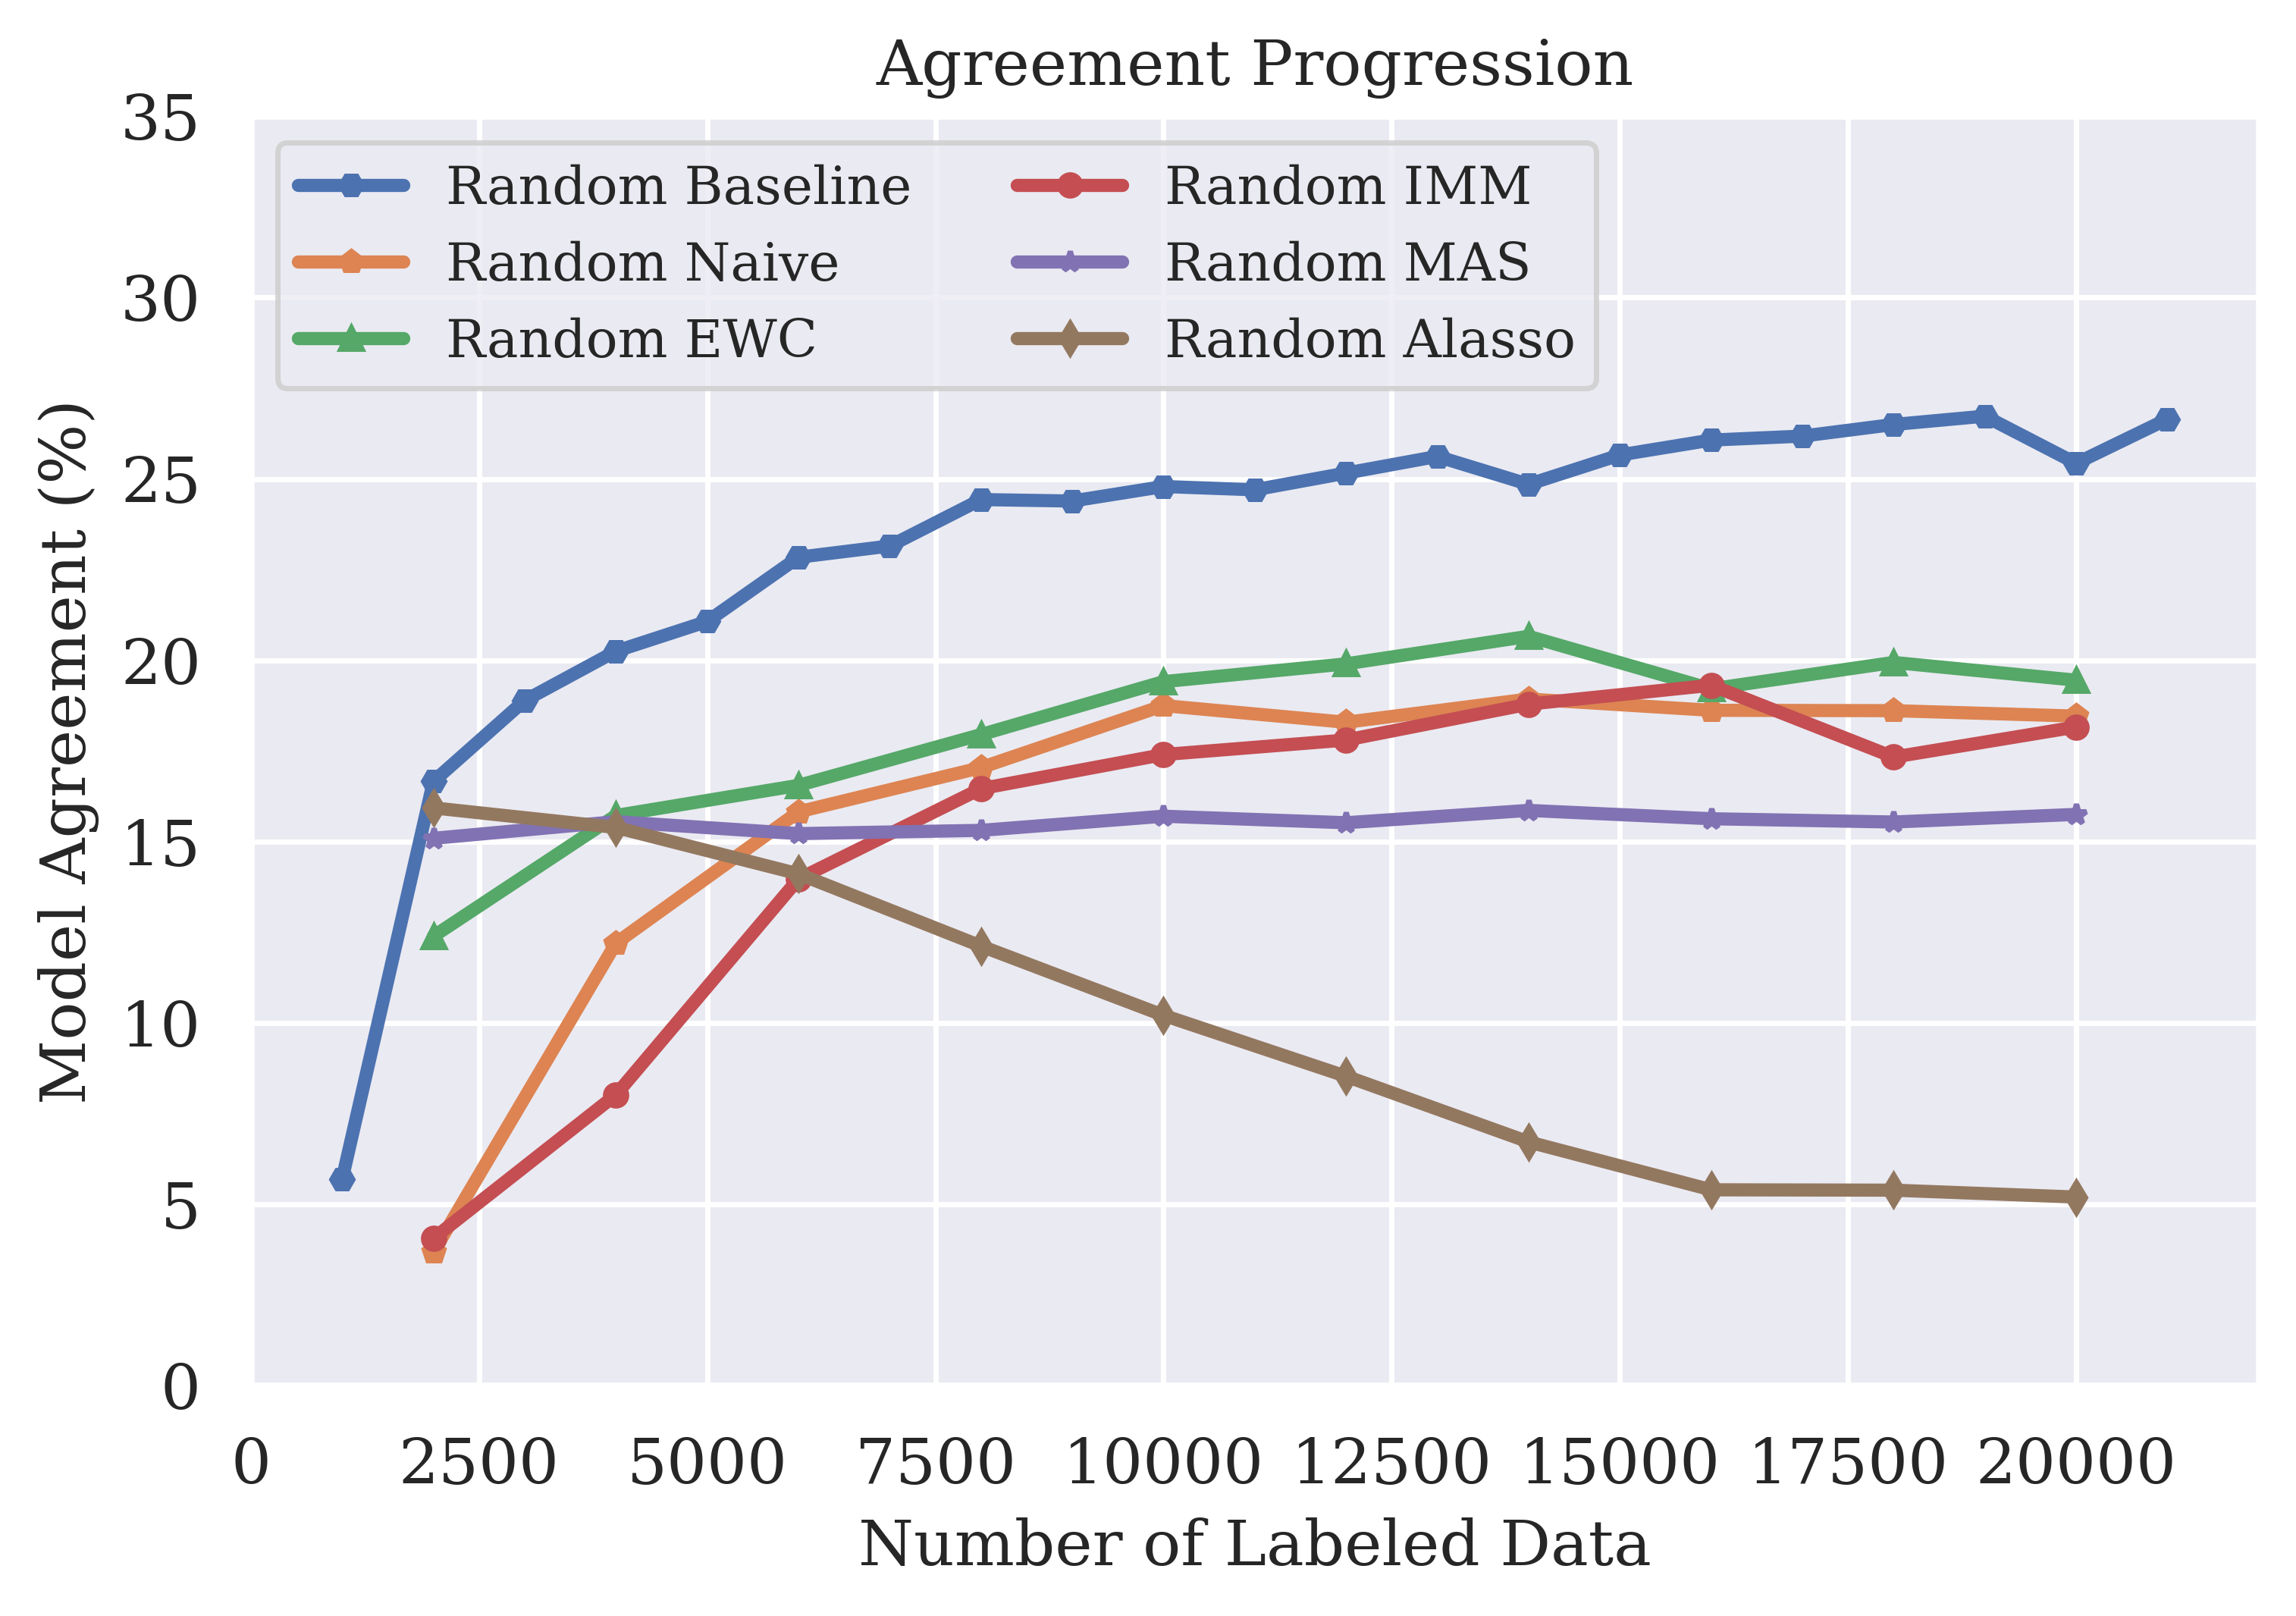
\includegraphics[width=0.48\linewidth]{images/results_CALMS/cifar100_softmax_random.png}
    \caption{Agreement Comparison for Model Stealing on CIFAR-10 using the Active Learning strategy Random. Left: Training with predicted class label,
    Right: Training with softmax output}
    \label{fig:CALMSCIFAR10Random}
\end{figure}

\begin{figure}[!htb]
    \centering
    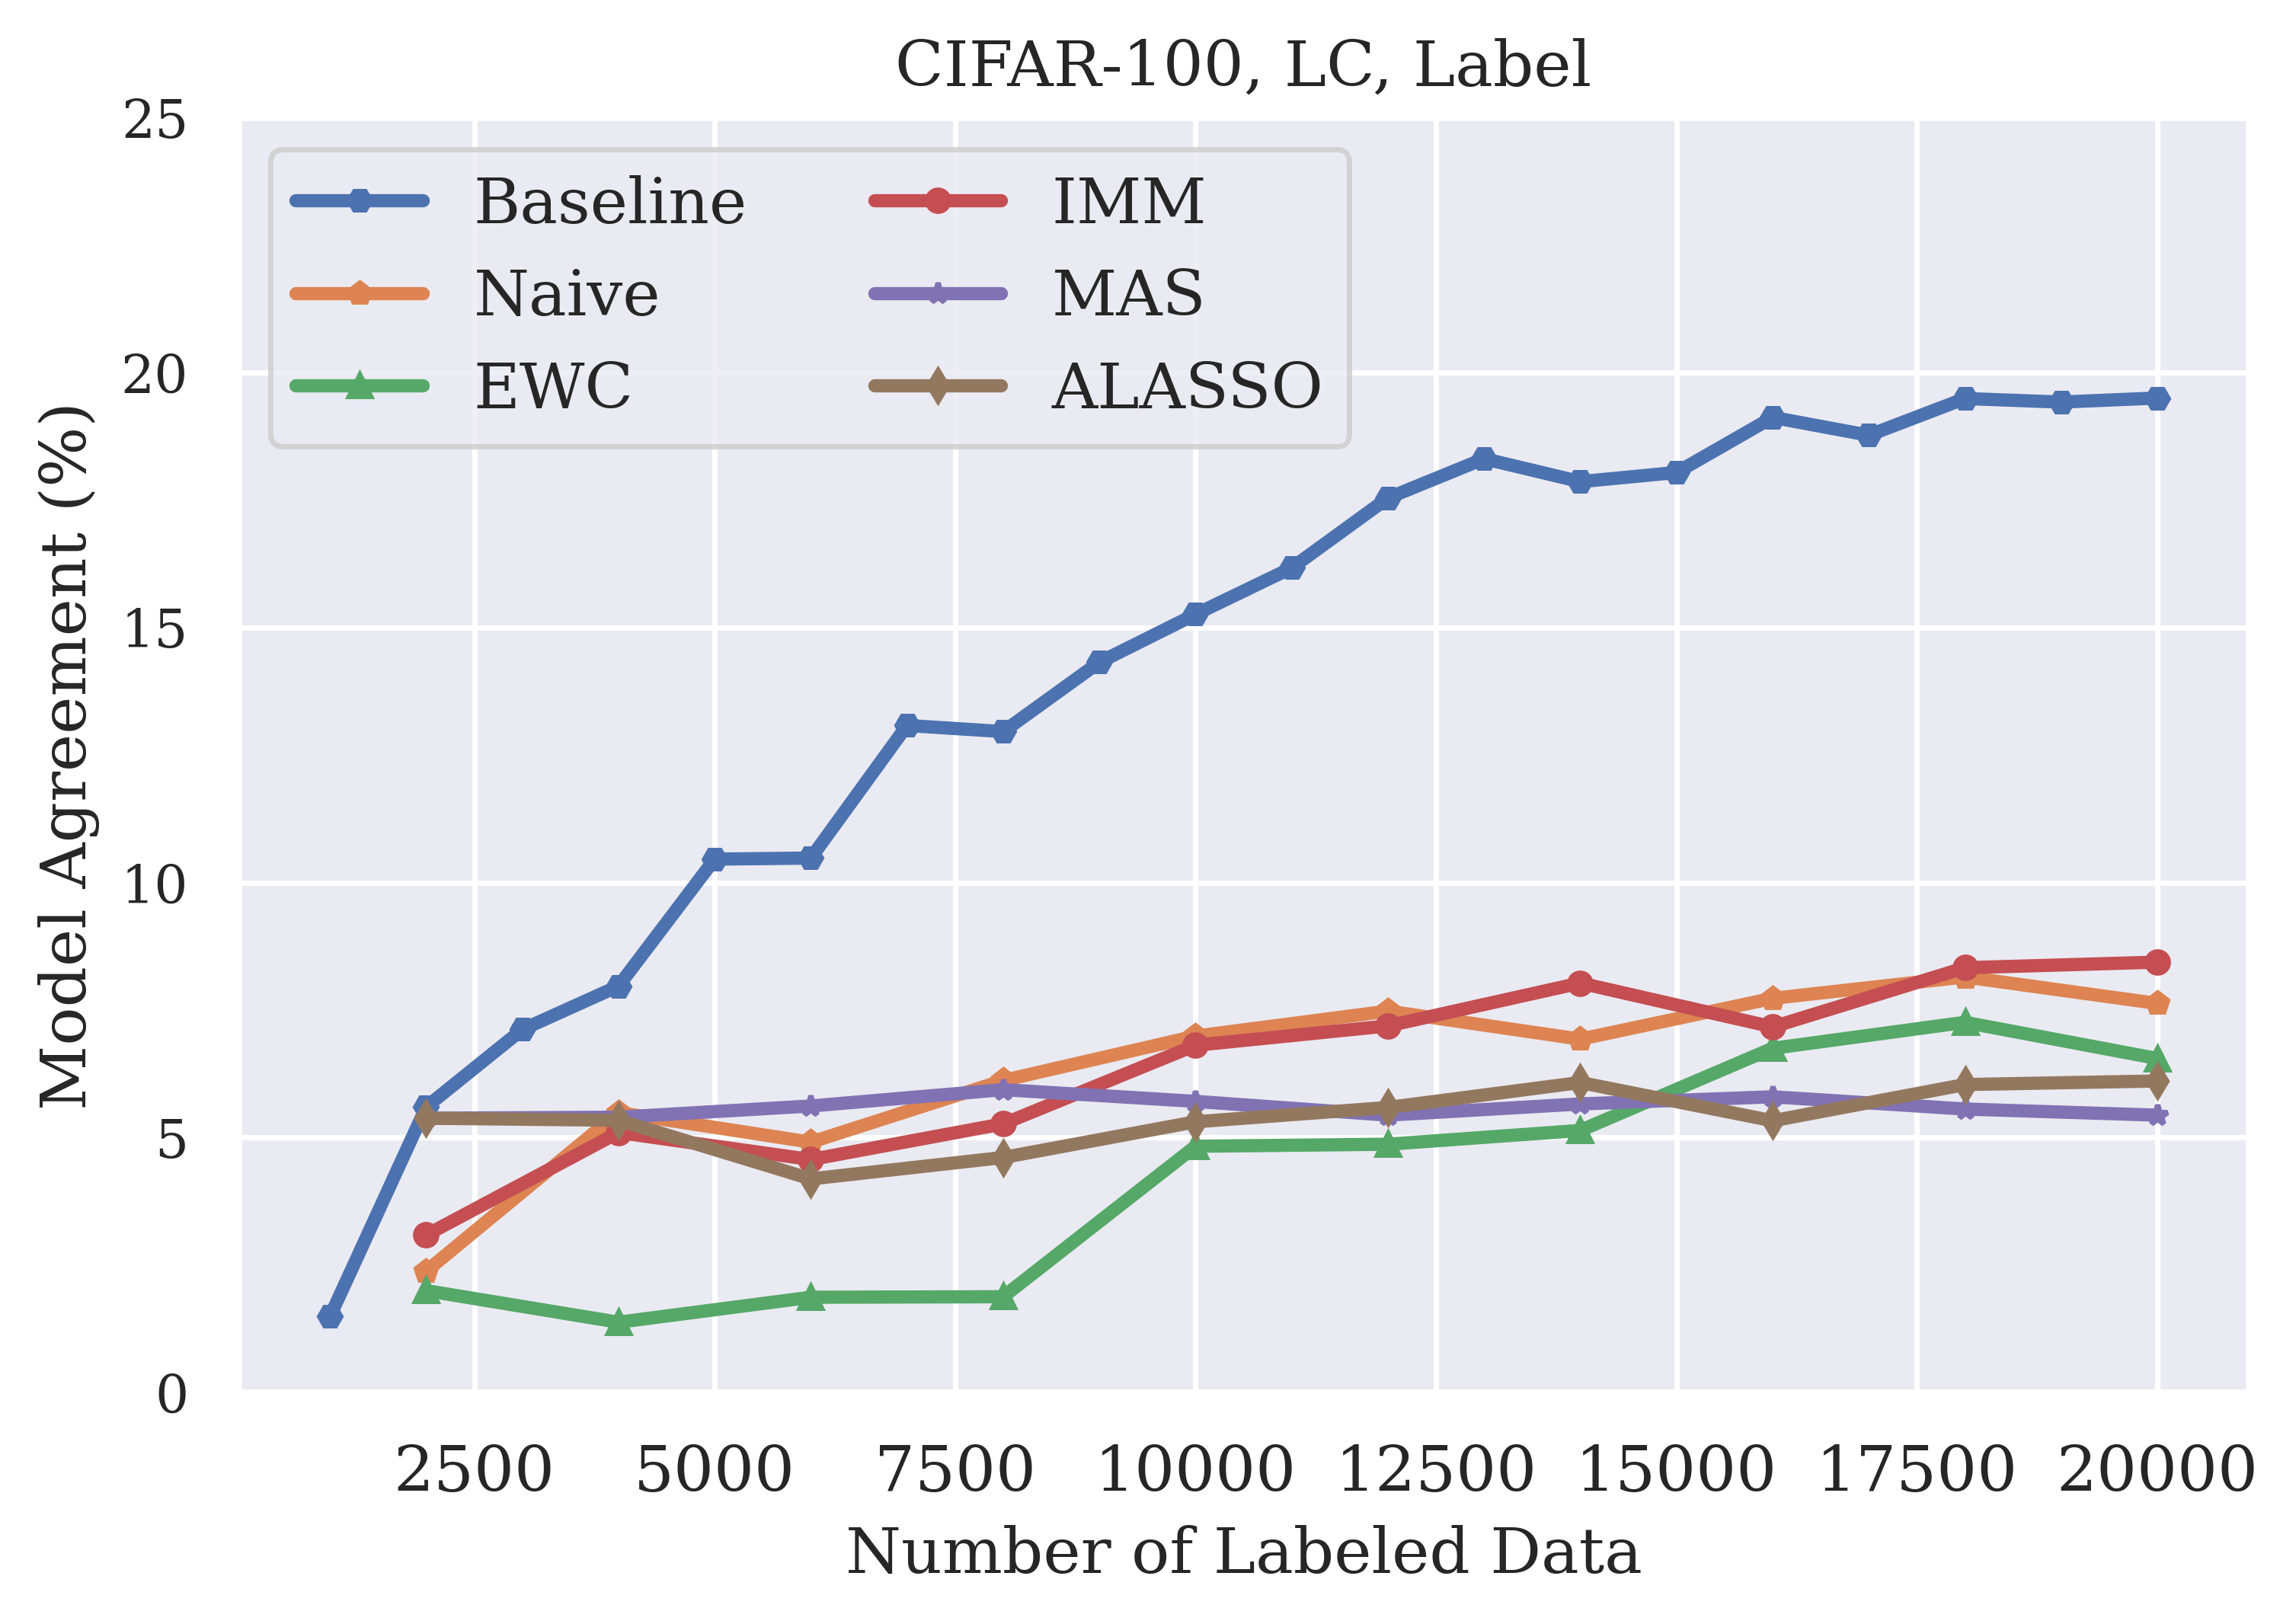
\includegraphics[width=0.48\linewidth]{images/results_CALMS/cifar100_label_lc.png} \hfill
    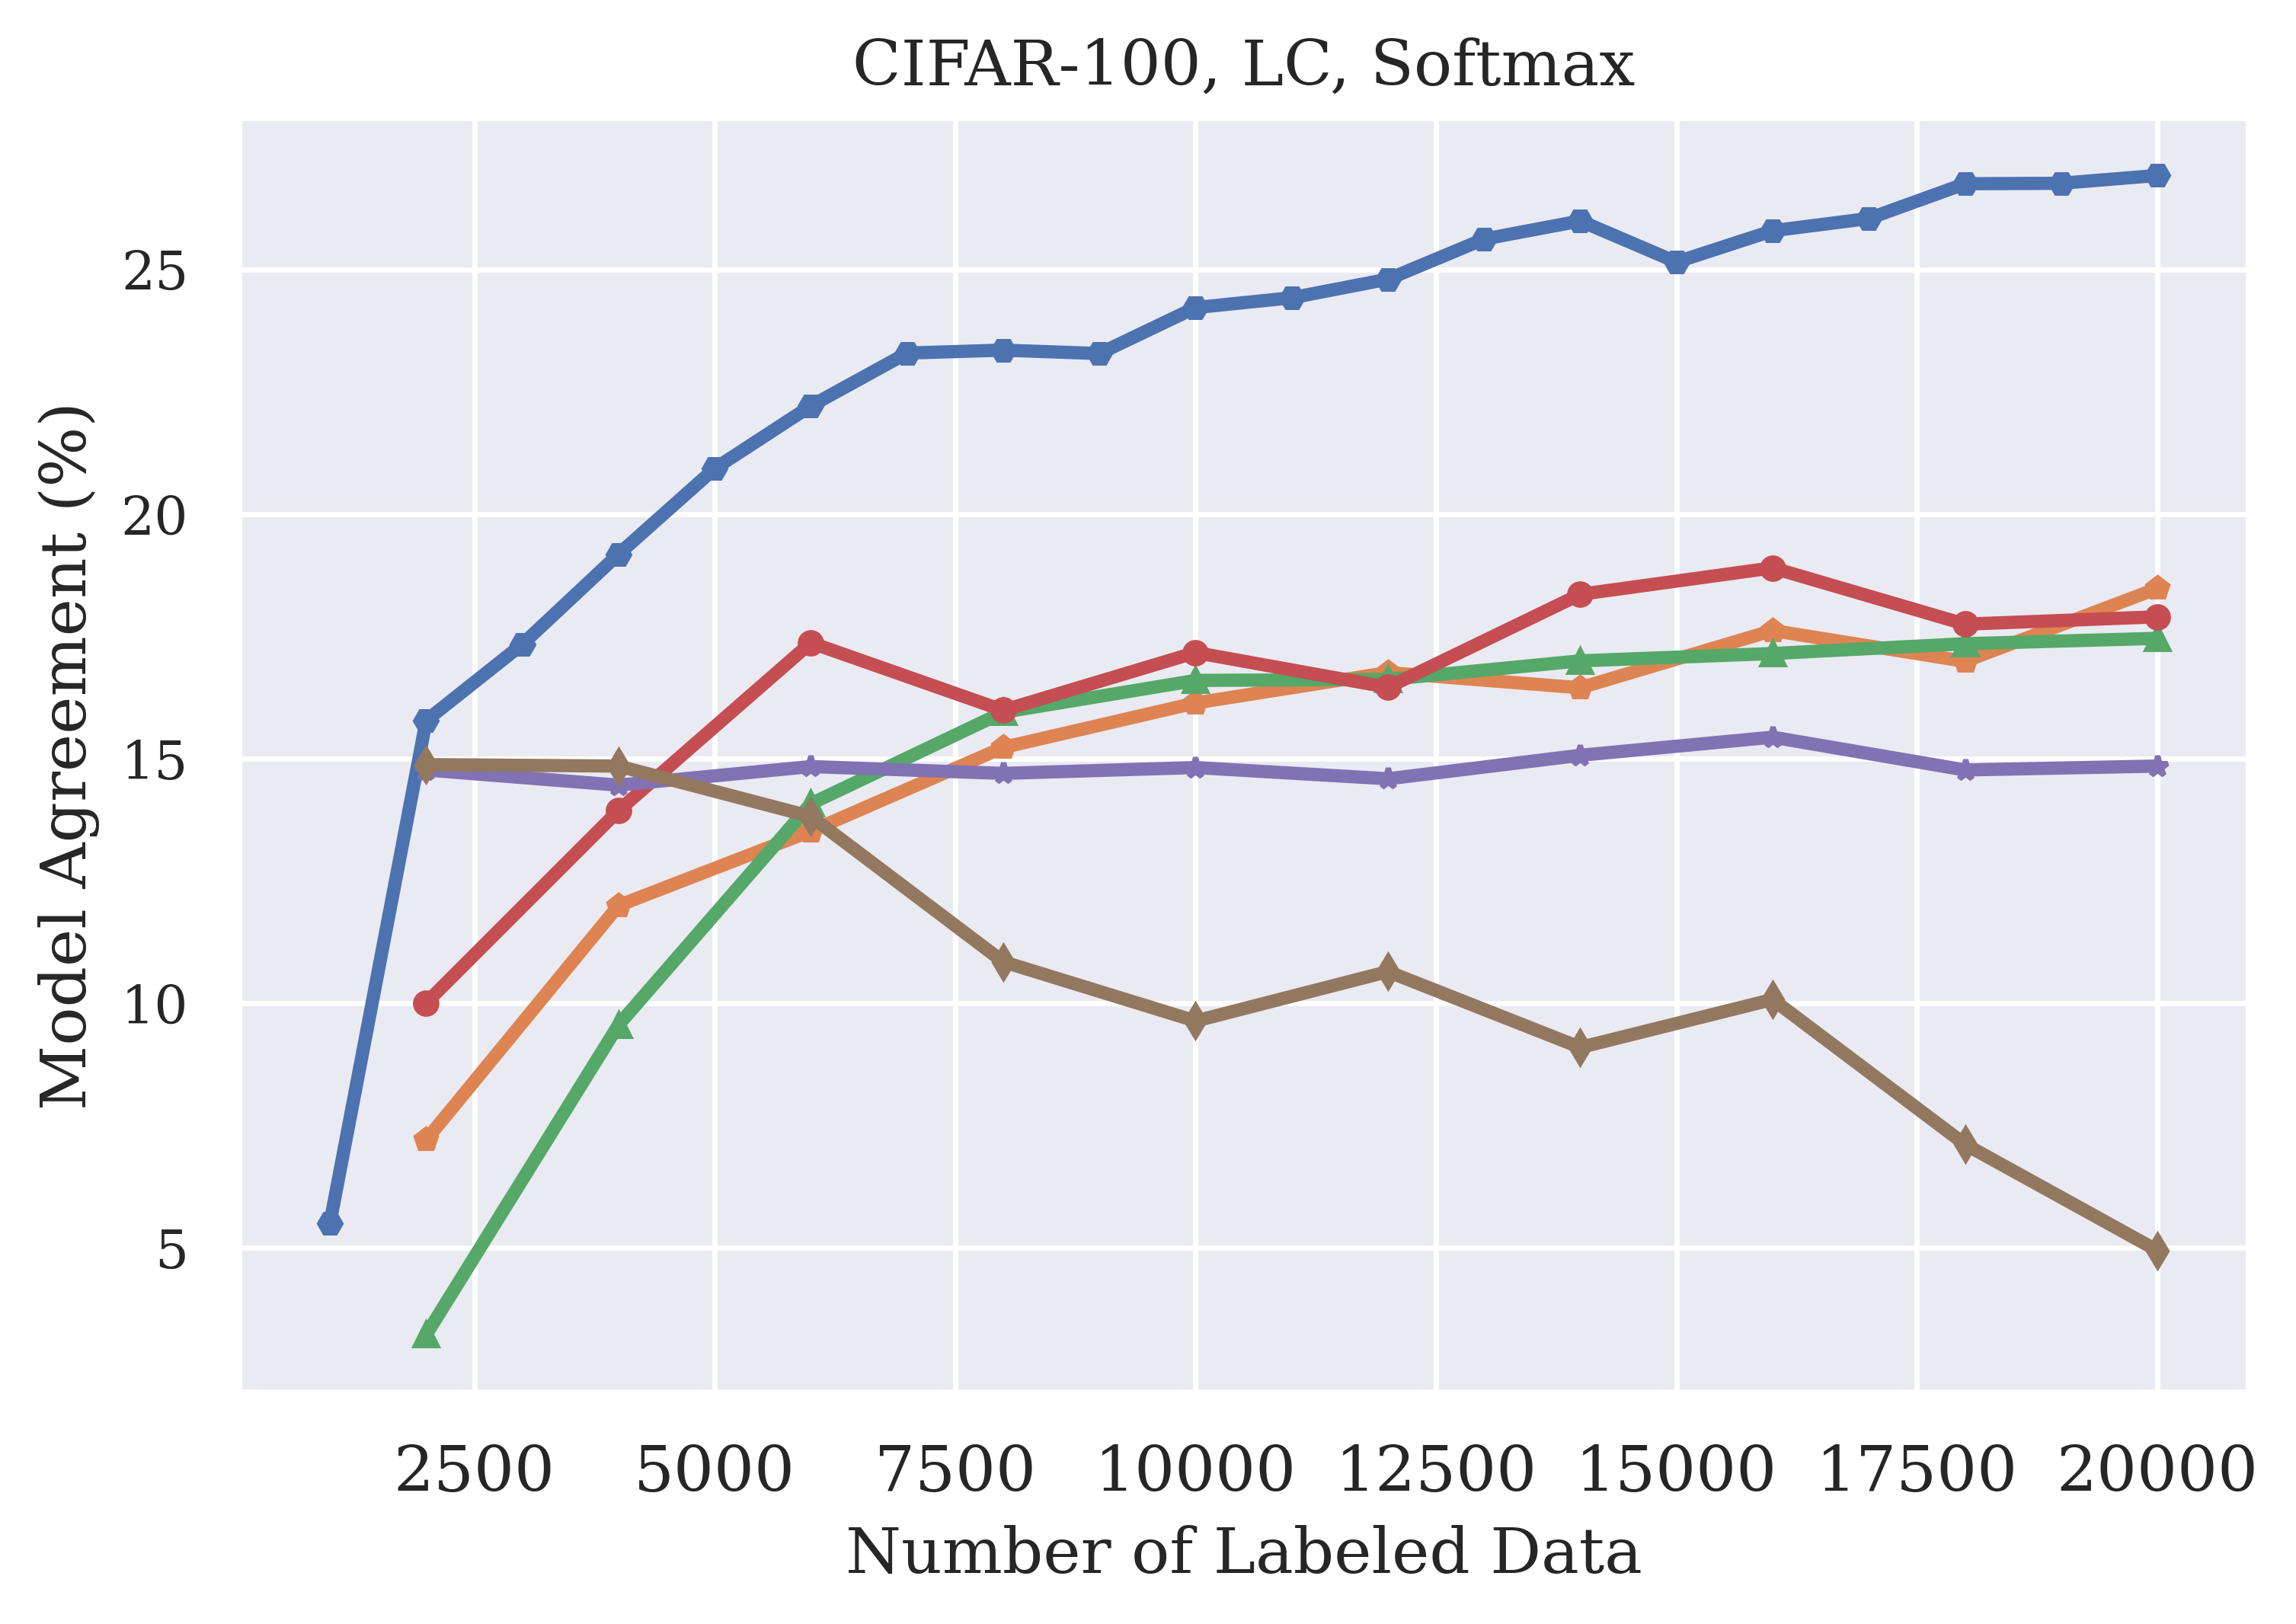
\includegraphics[width=0.48\linewidth]{images/results_CALMS/cifar100_softmax_lc.png}
    \caption{Agreement Comparison for Model Stealing on CIFAR10 using the Active Learning strategy \gls{lc}. Left: Training with predicted class label,
    Right: Training with softmax output}
    \label{fig:CALMSCIFAR10LC}
\end{figure}

\begin{figure}[!htb]
    \centering
    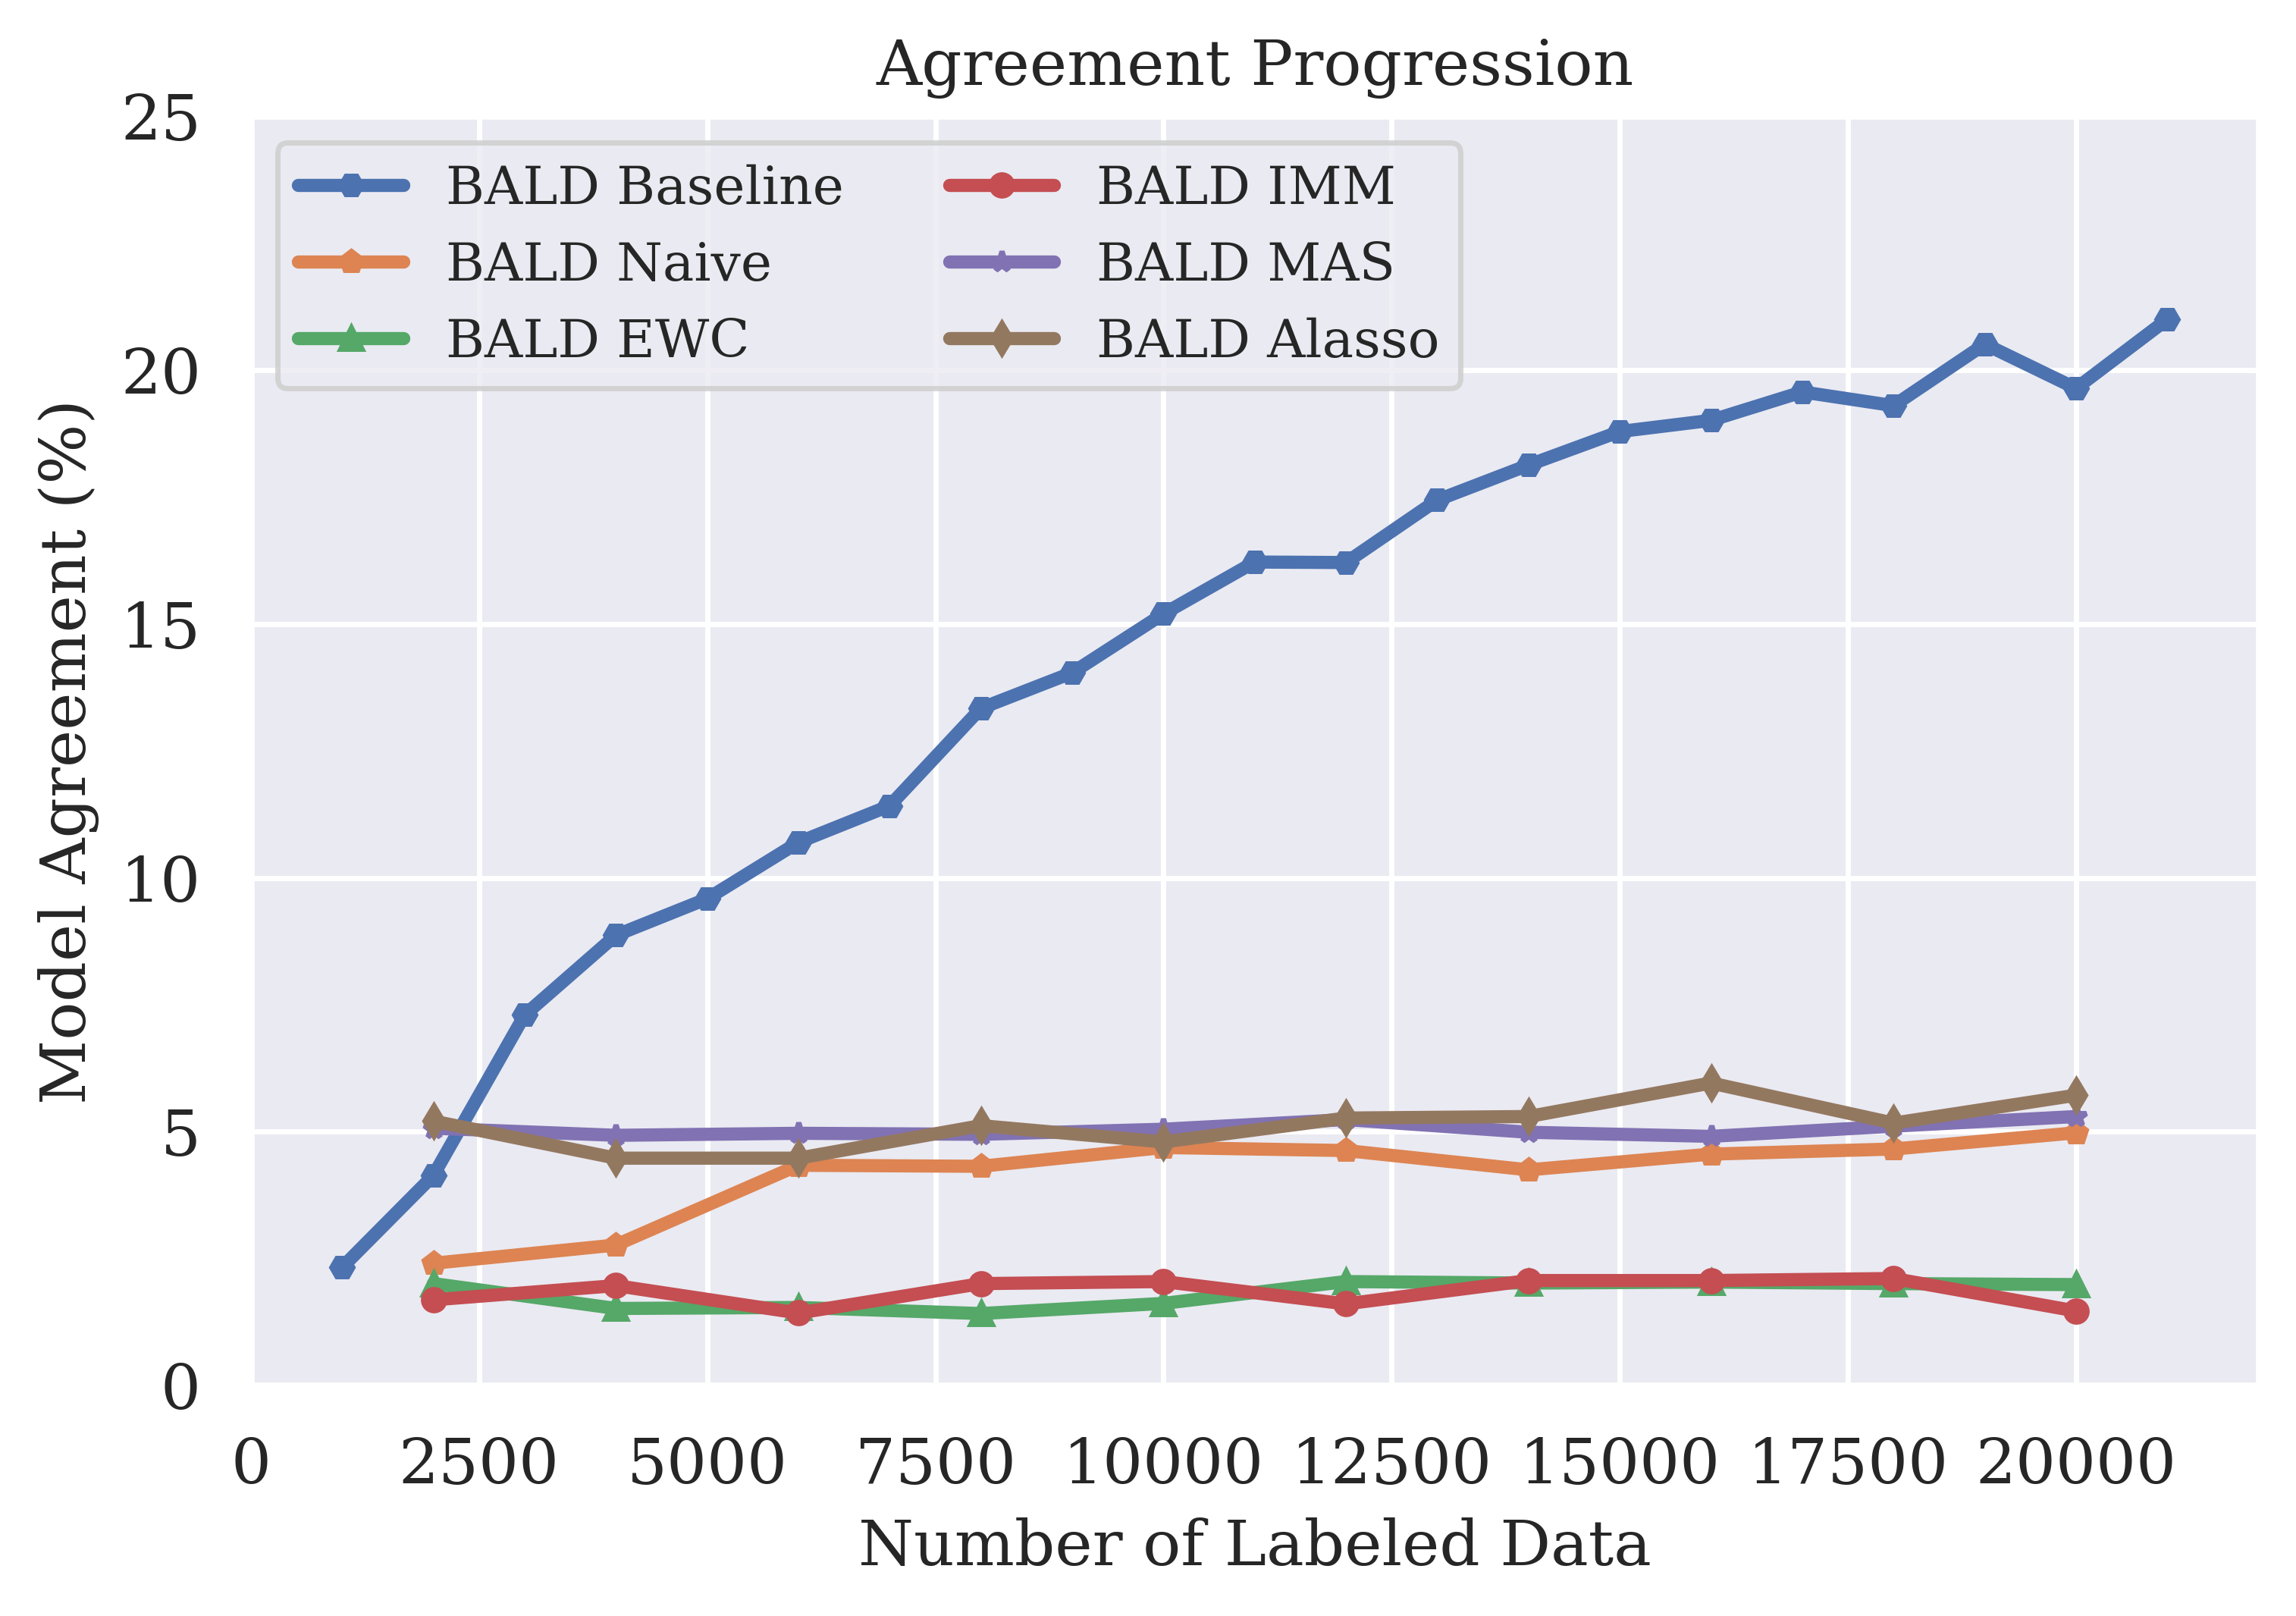
\includegraphics[width=0.48\linewidth]{images/results_CALMS/cifar100_label_bald.png} \hfill
    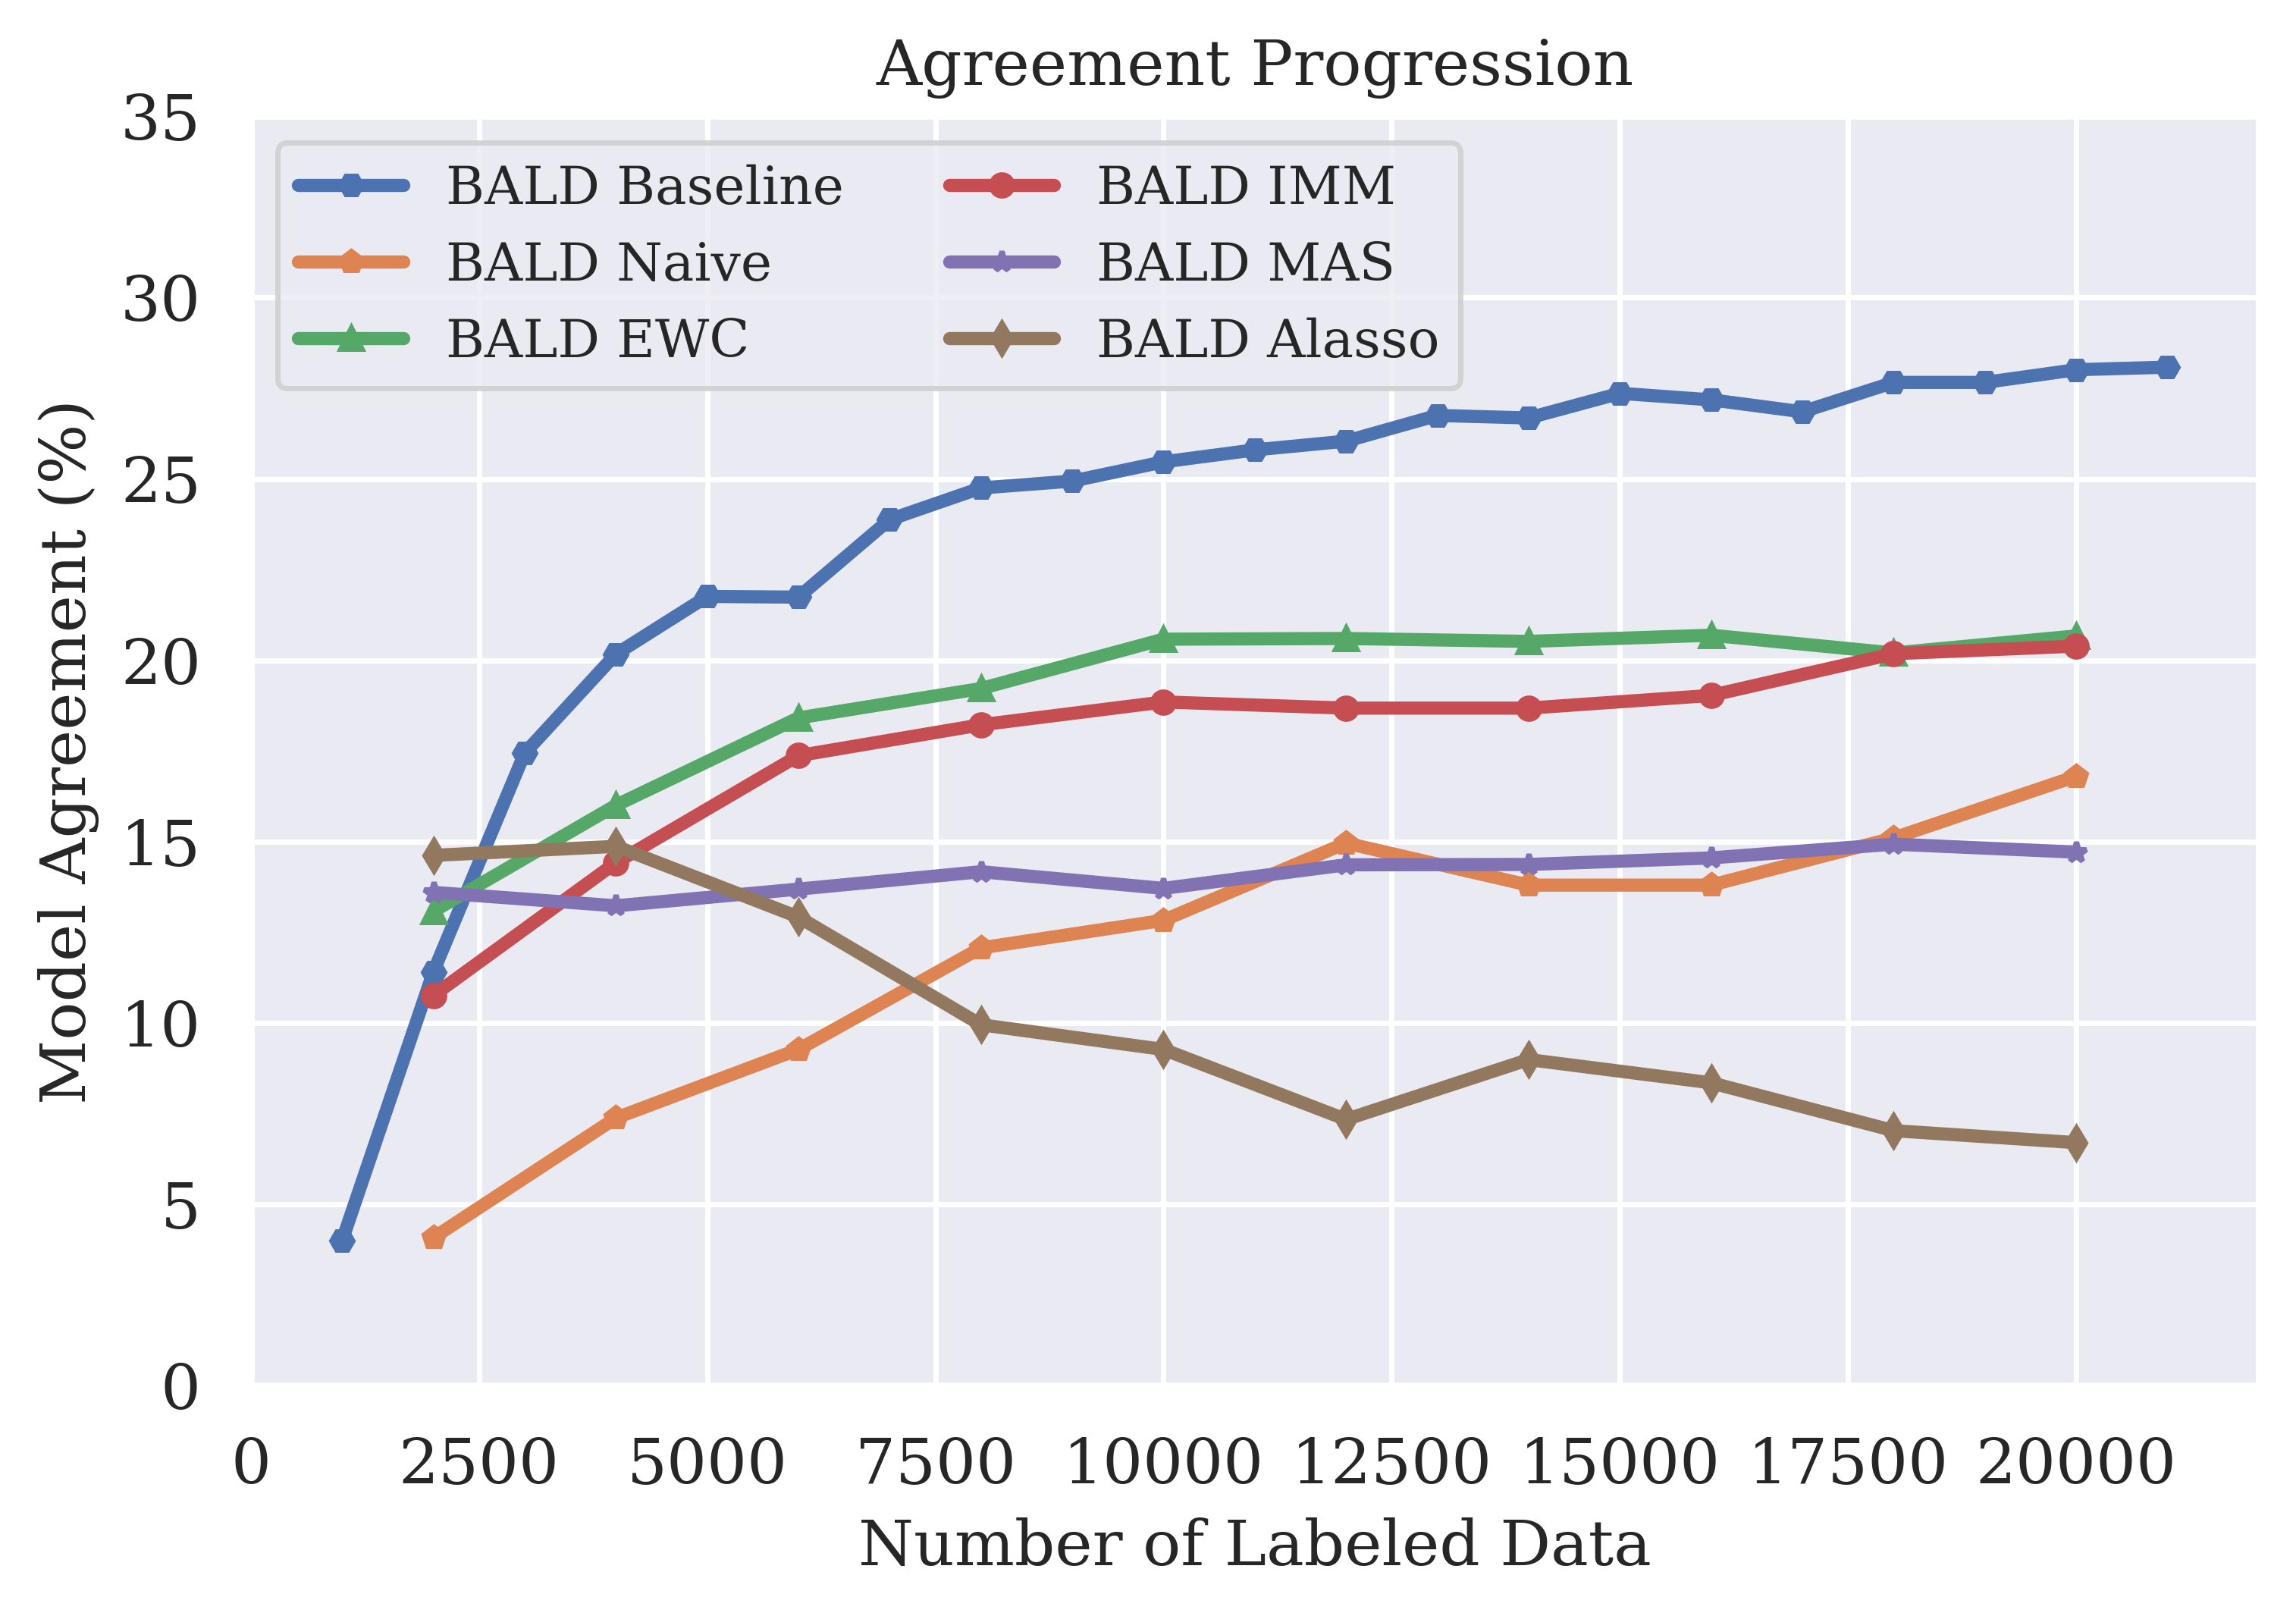
\includegraphics[width=0.48\linewidth]{images/results_CALMS/cifar100_softmax_bald.png}
    \caption{Agreement Comparison for Model Stealing on CIFAR-10 using the Active Learning strategy \gls{bald}. Left: Training with predicted class label,
    Right: Training with softmax output}
    \label{fig:CALMSCIFAR10BALD}
\end{figure}

\begin{figure}[!htb]
    \centering
    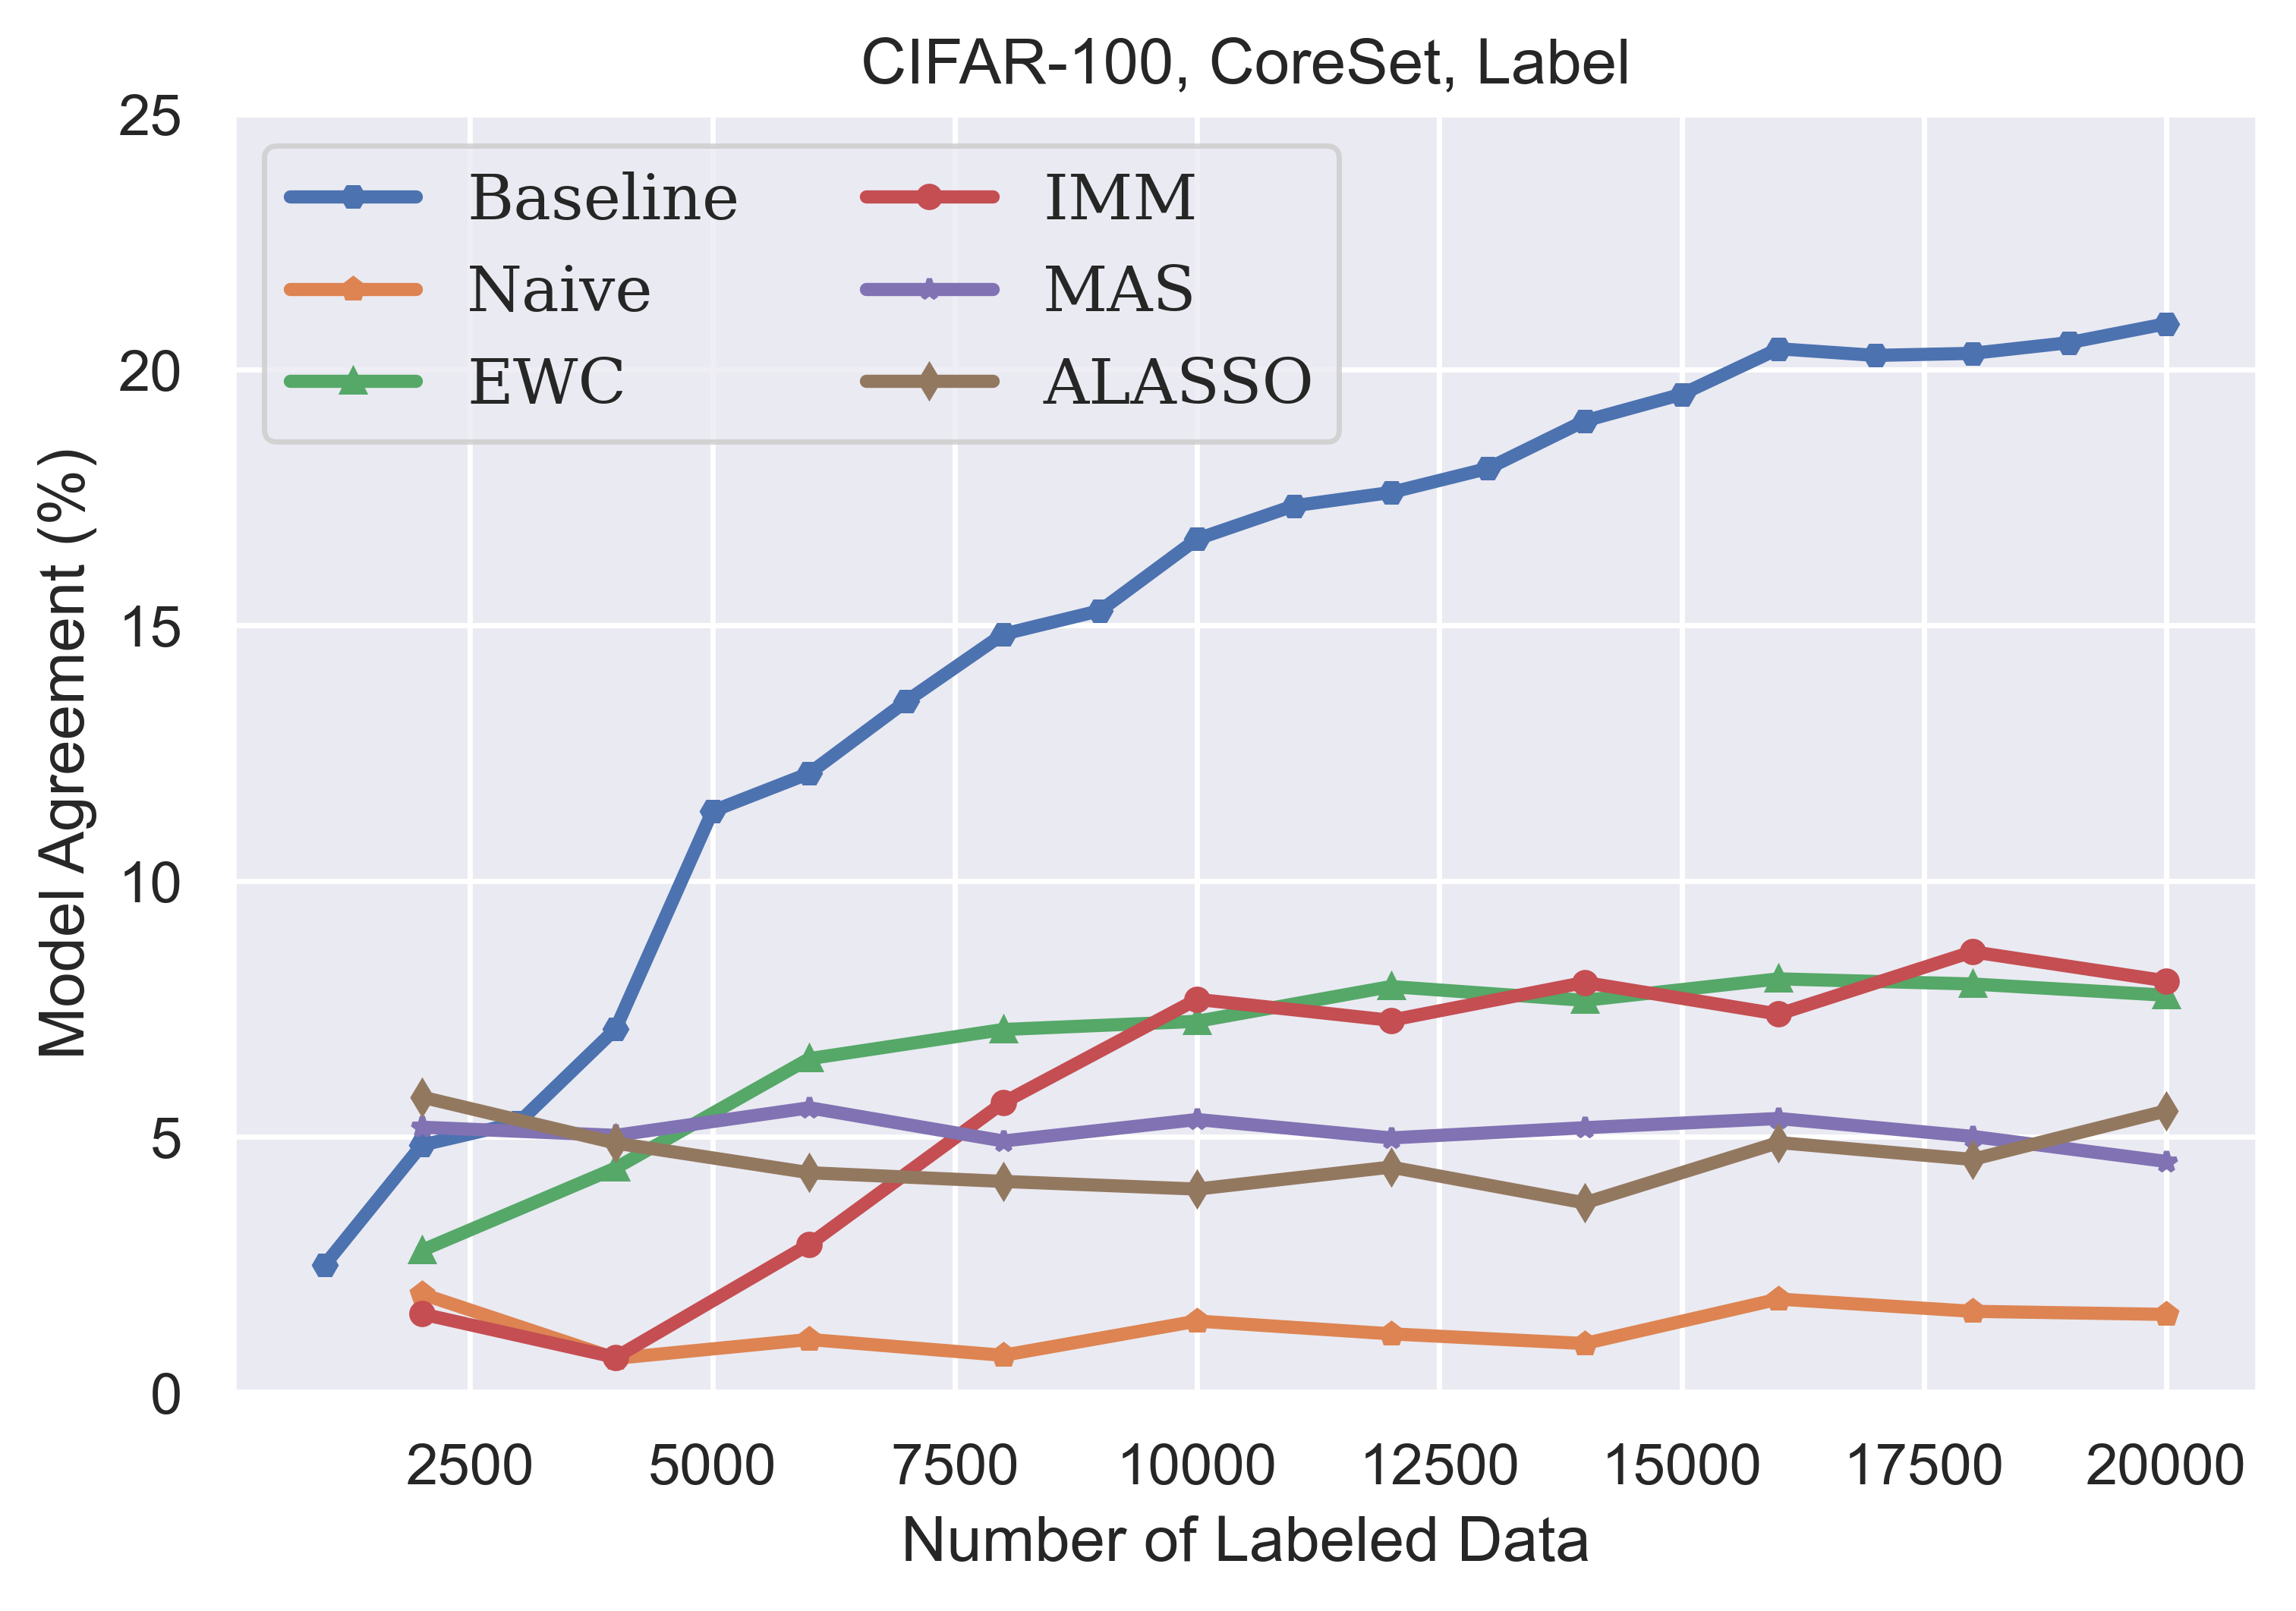
\includegraphics[width=0.48\linewidth]{images/results_CALMS/cifar100_label_coreset.png} \hfill
    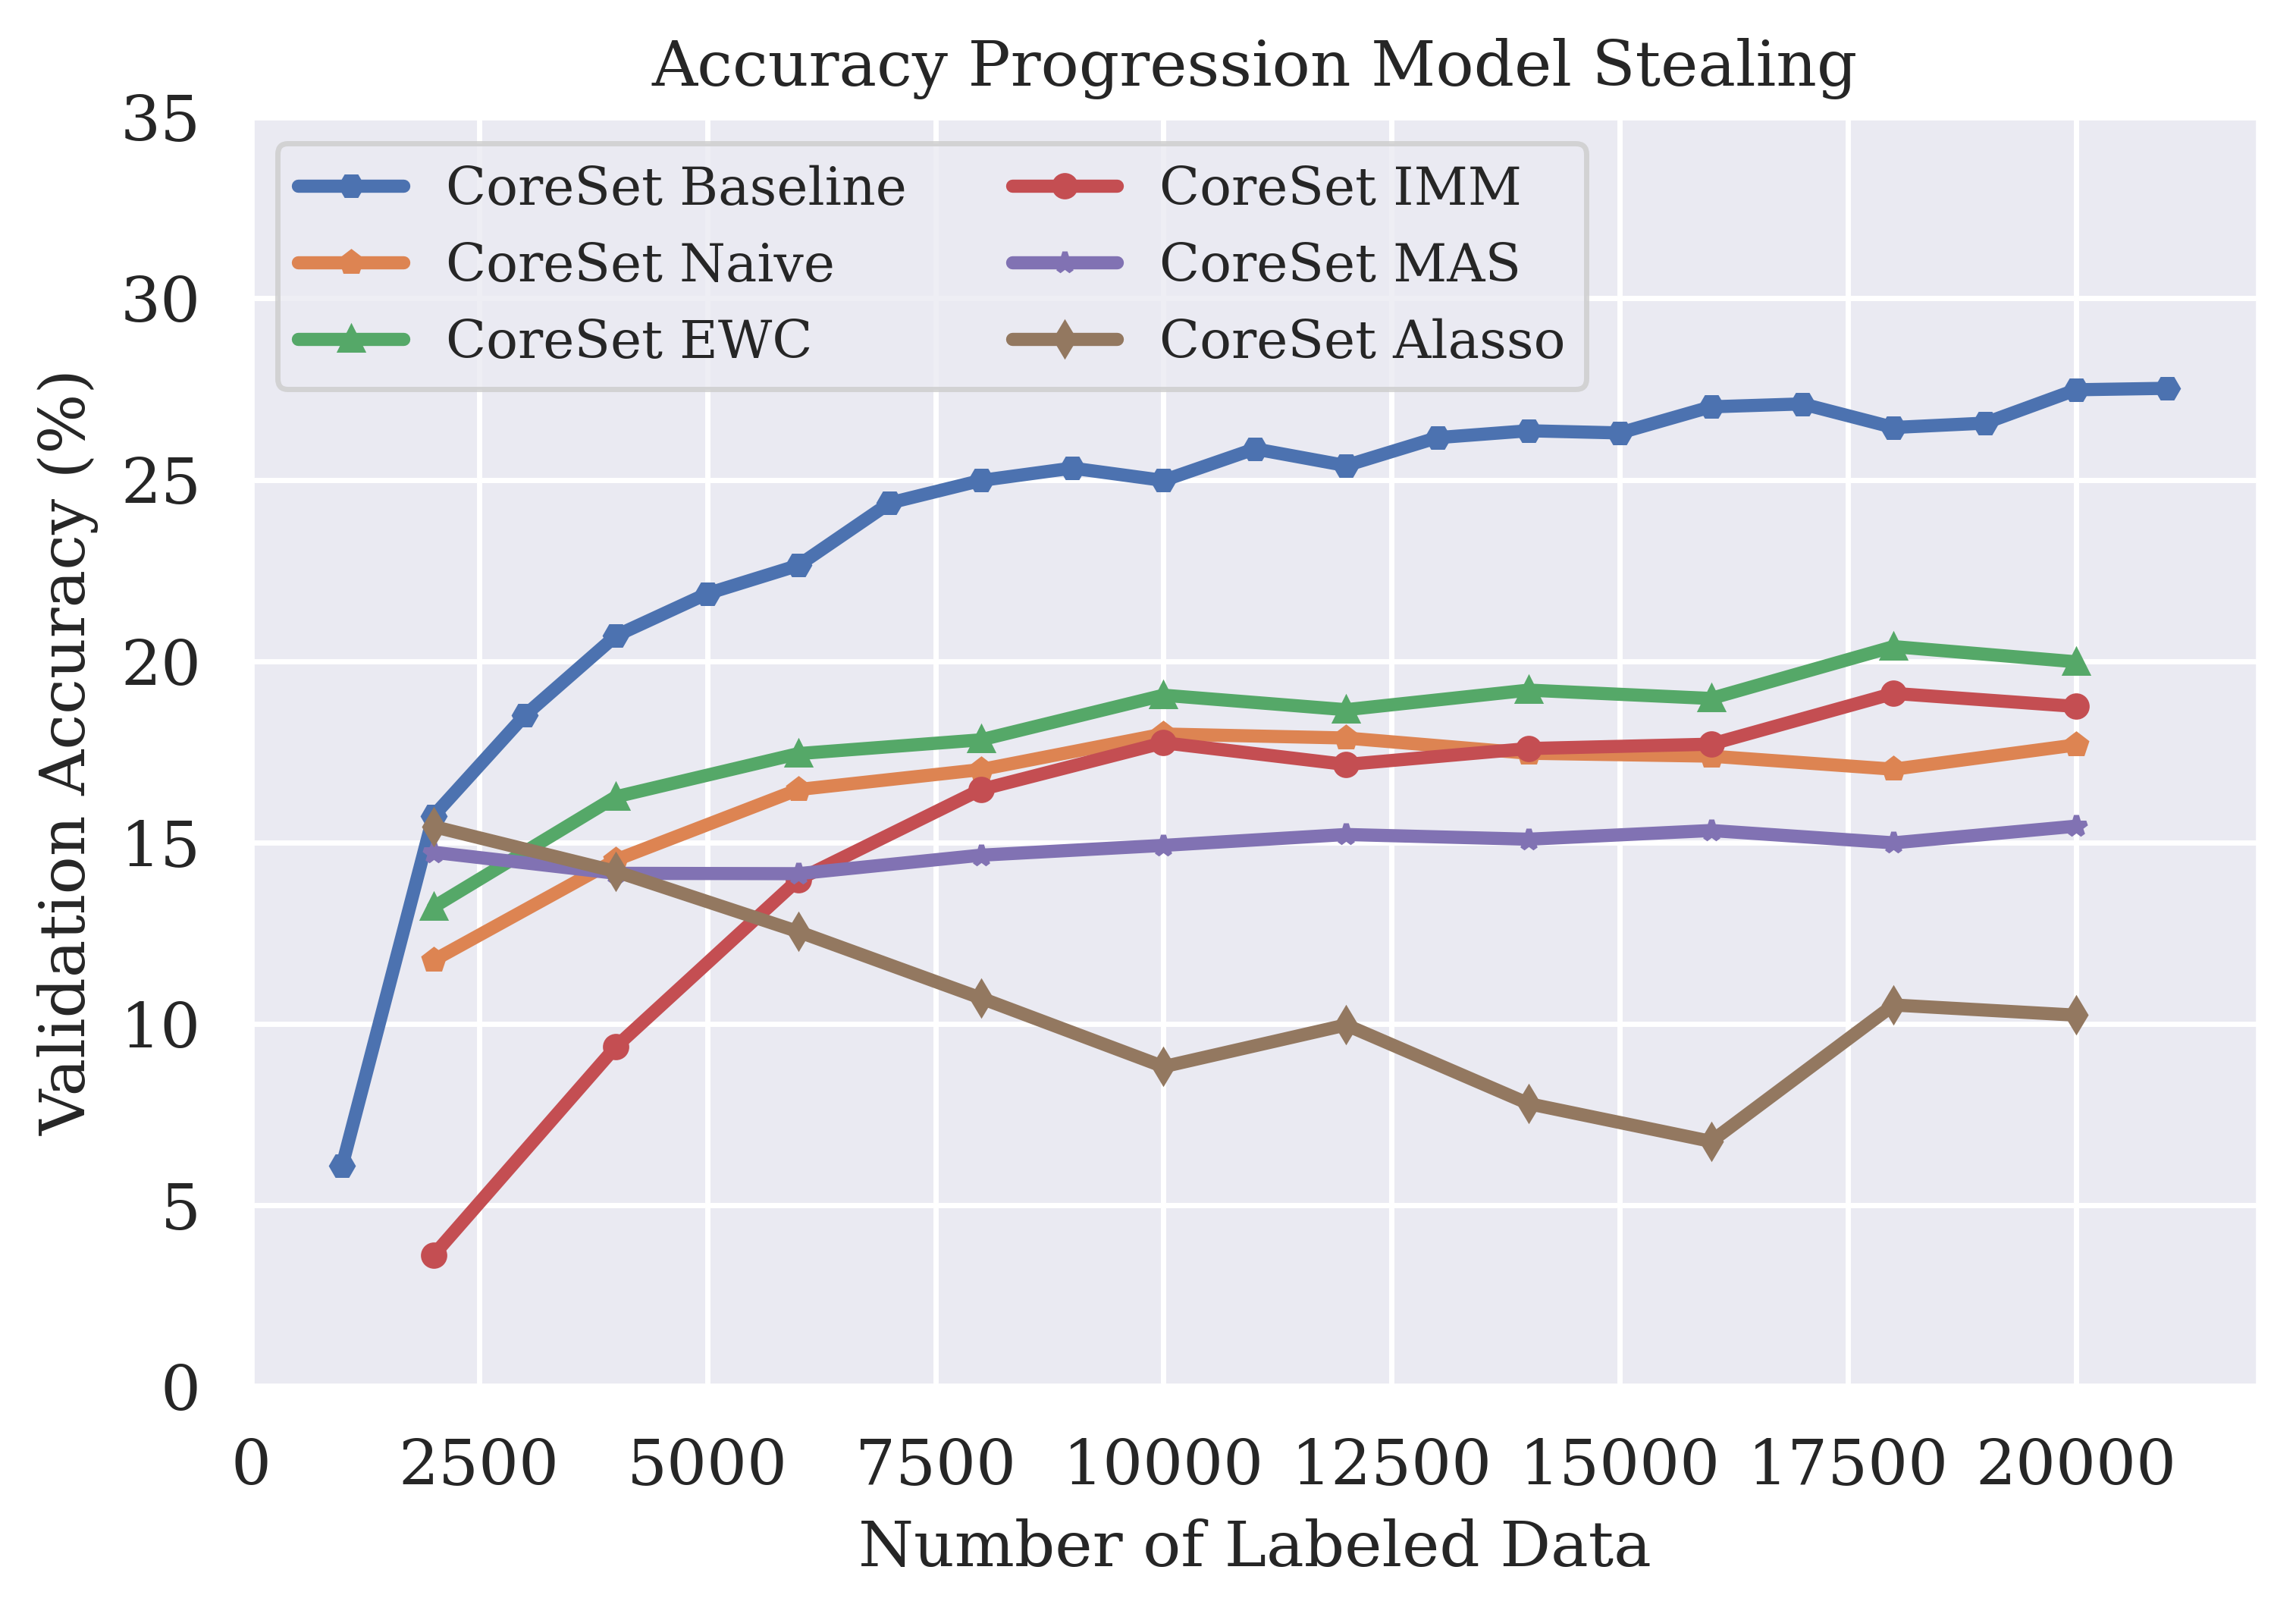
\includegraphics[width=0.48\linewidth]{images/results_CALMS/cifar100_softmax_coreset.png}
    \caption{Agreement Comparison for Model Stealing on CIFAR-10 using the Active Learning strategy CoreSet. Left: Training with predicted class label,
    Right: Training with softmax output}
    \label{fig:CALMSCIFAR10CoreSet}
\end{figure}

\begin{figure}[!htb]
    \centering
    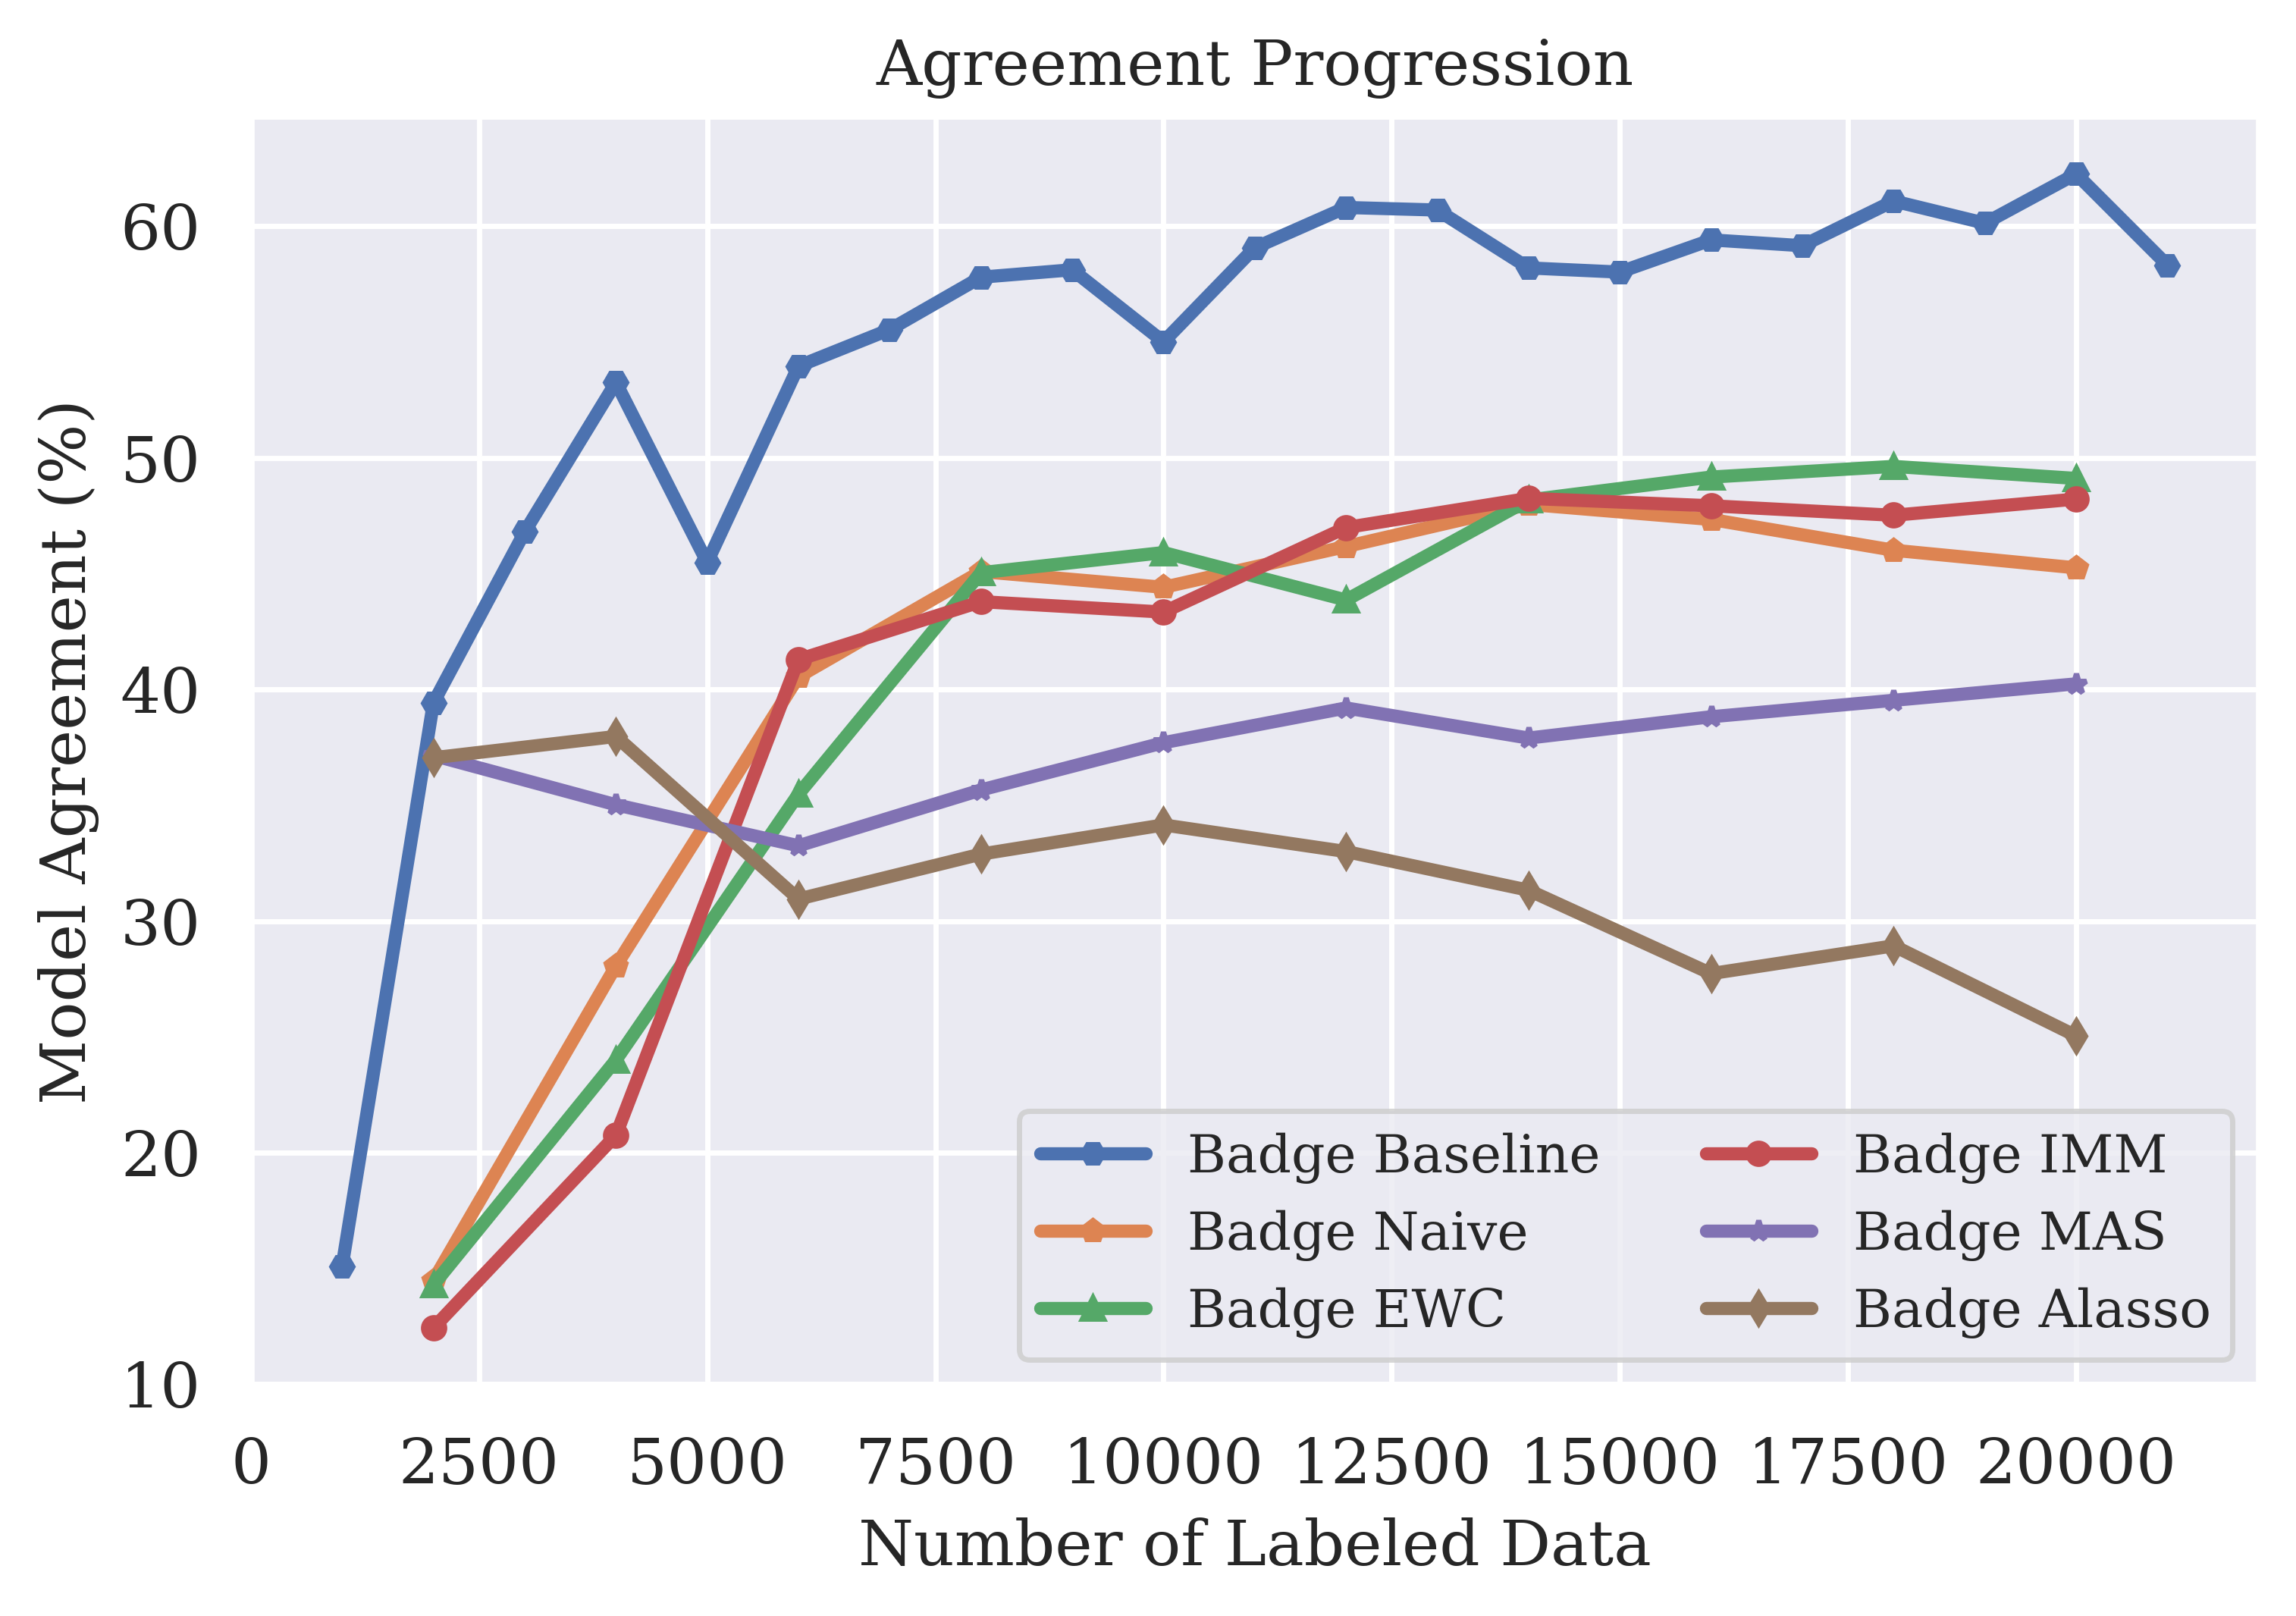
\includegraphics[width=0.48\linewidth]{images/results_CALMS/cifar_label_badge.png} \hfill
    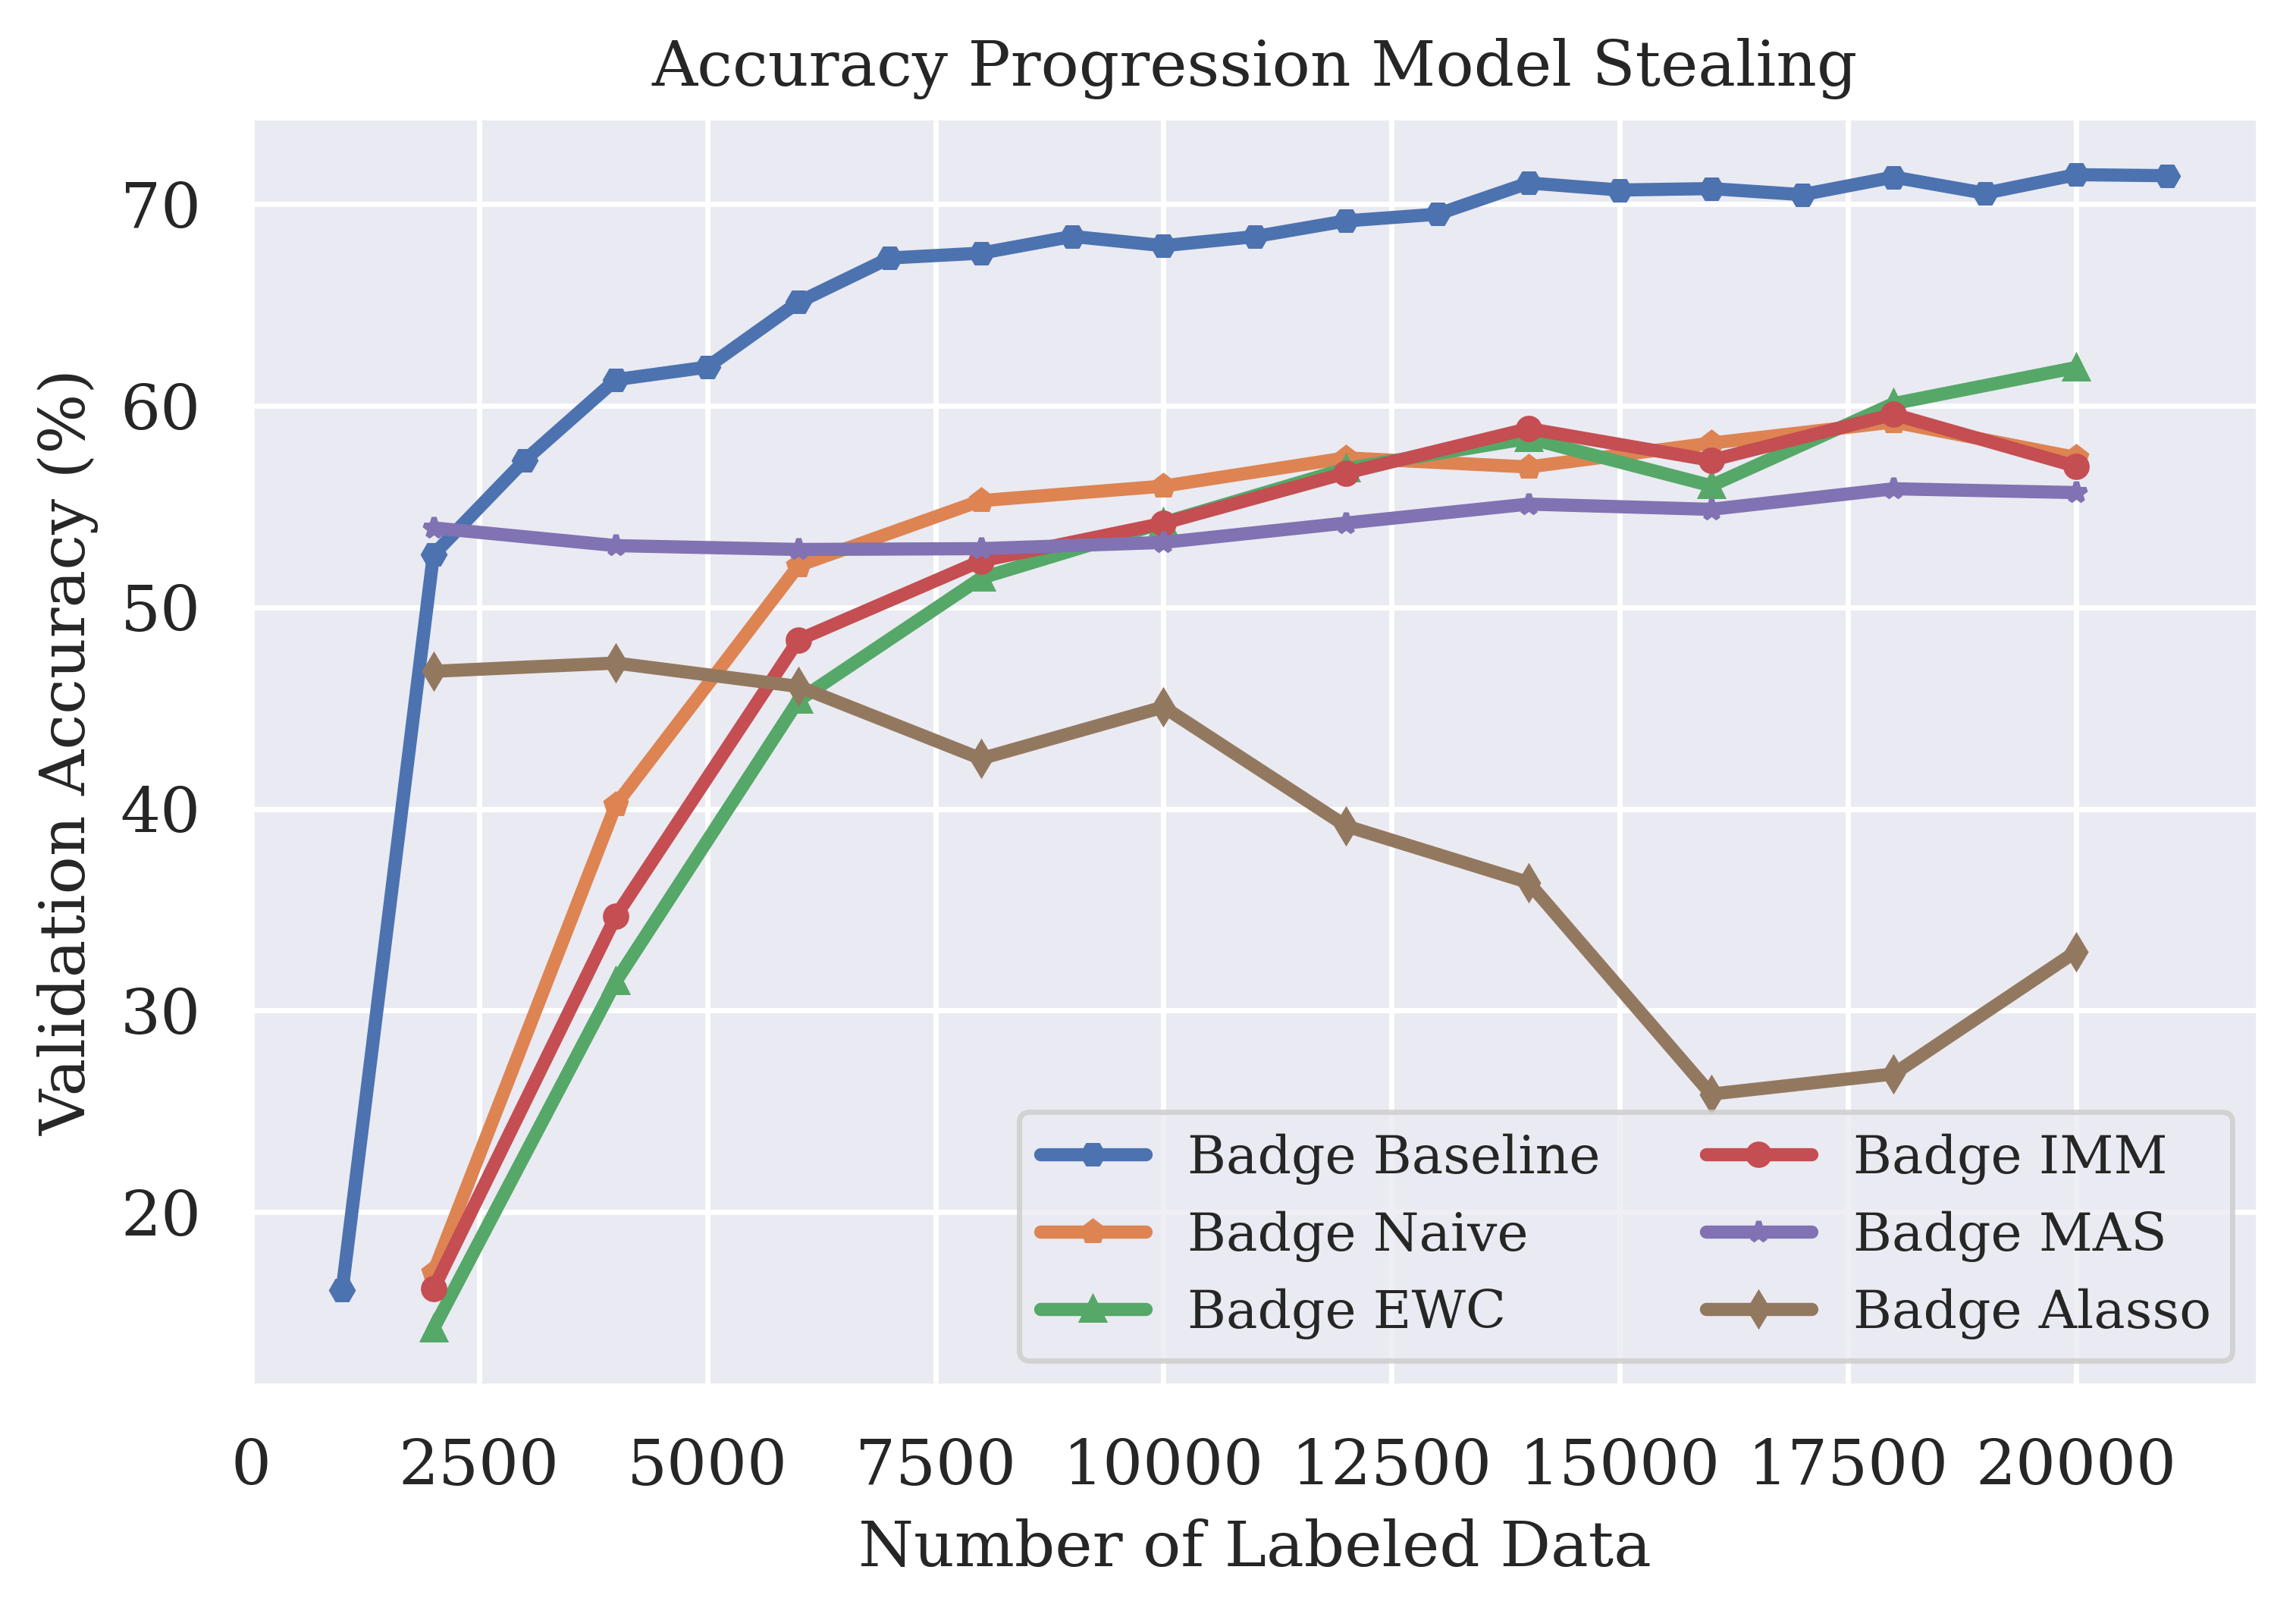
\includegraphics[width=0.48\linewidth]{images/results_CALMS/cifar_softmax_badge.png}
    \caption{Agreement Comparison for Model Stealing on CIFAR-10 using the Active Learning strategy \gls{badge}. Left: Training with predicted class label,
    Right: Training with softmax output}
    \label{fig:CALMSCIFAR10Badge}
\end{figure}


\subsubsection{CIFAR-100}
\label{sec:Appendix:CALMS:CIFAR100}
In this section, we present the full runs of all experiments which involve Continual Active Learning using CIFAR-100 as a Target Model Dataset.

\begin{figure}[!htb]
    \centering
    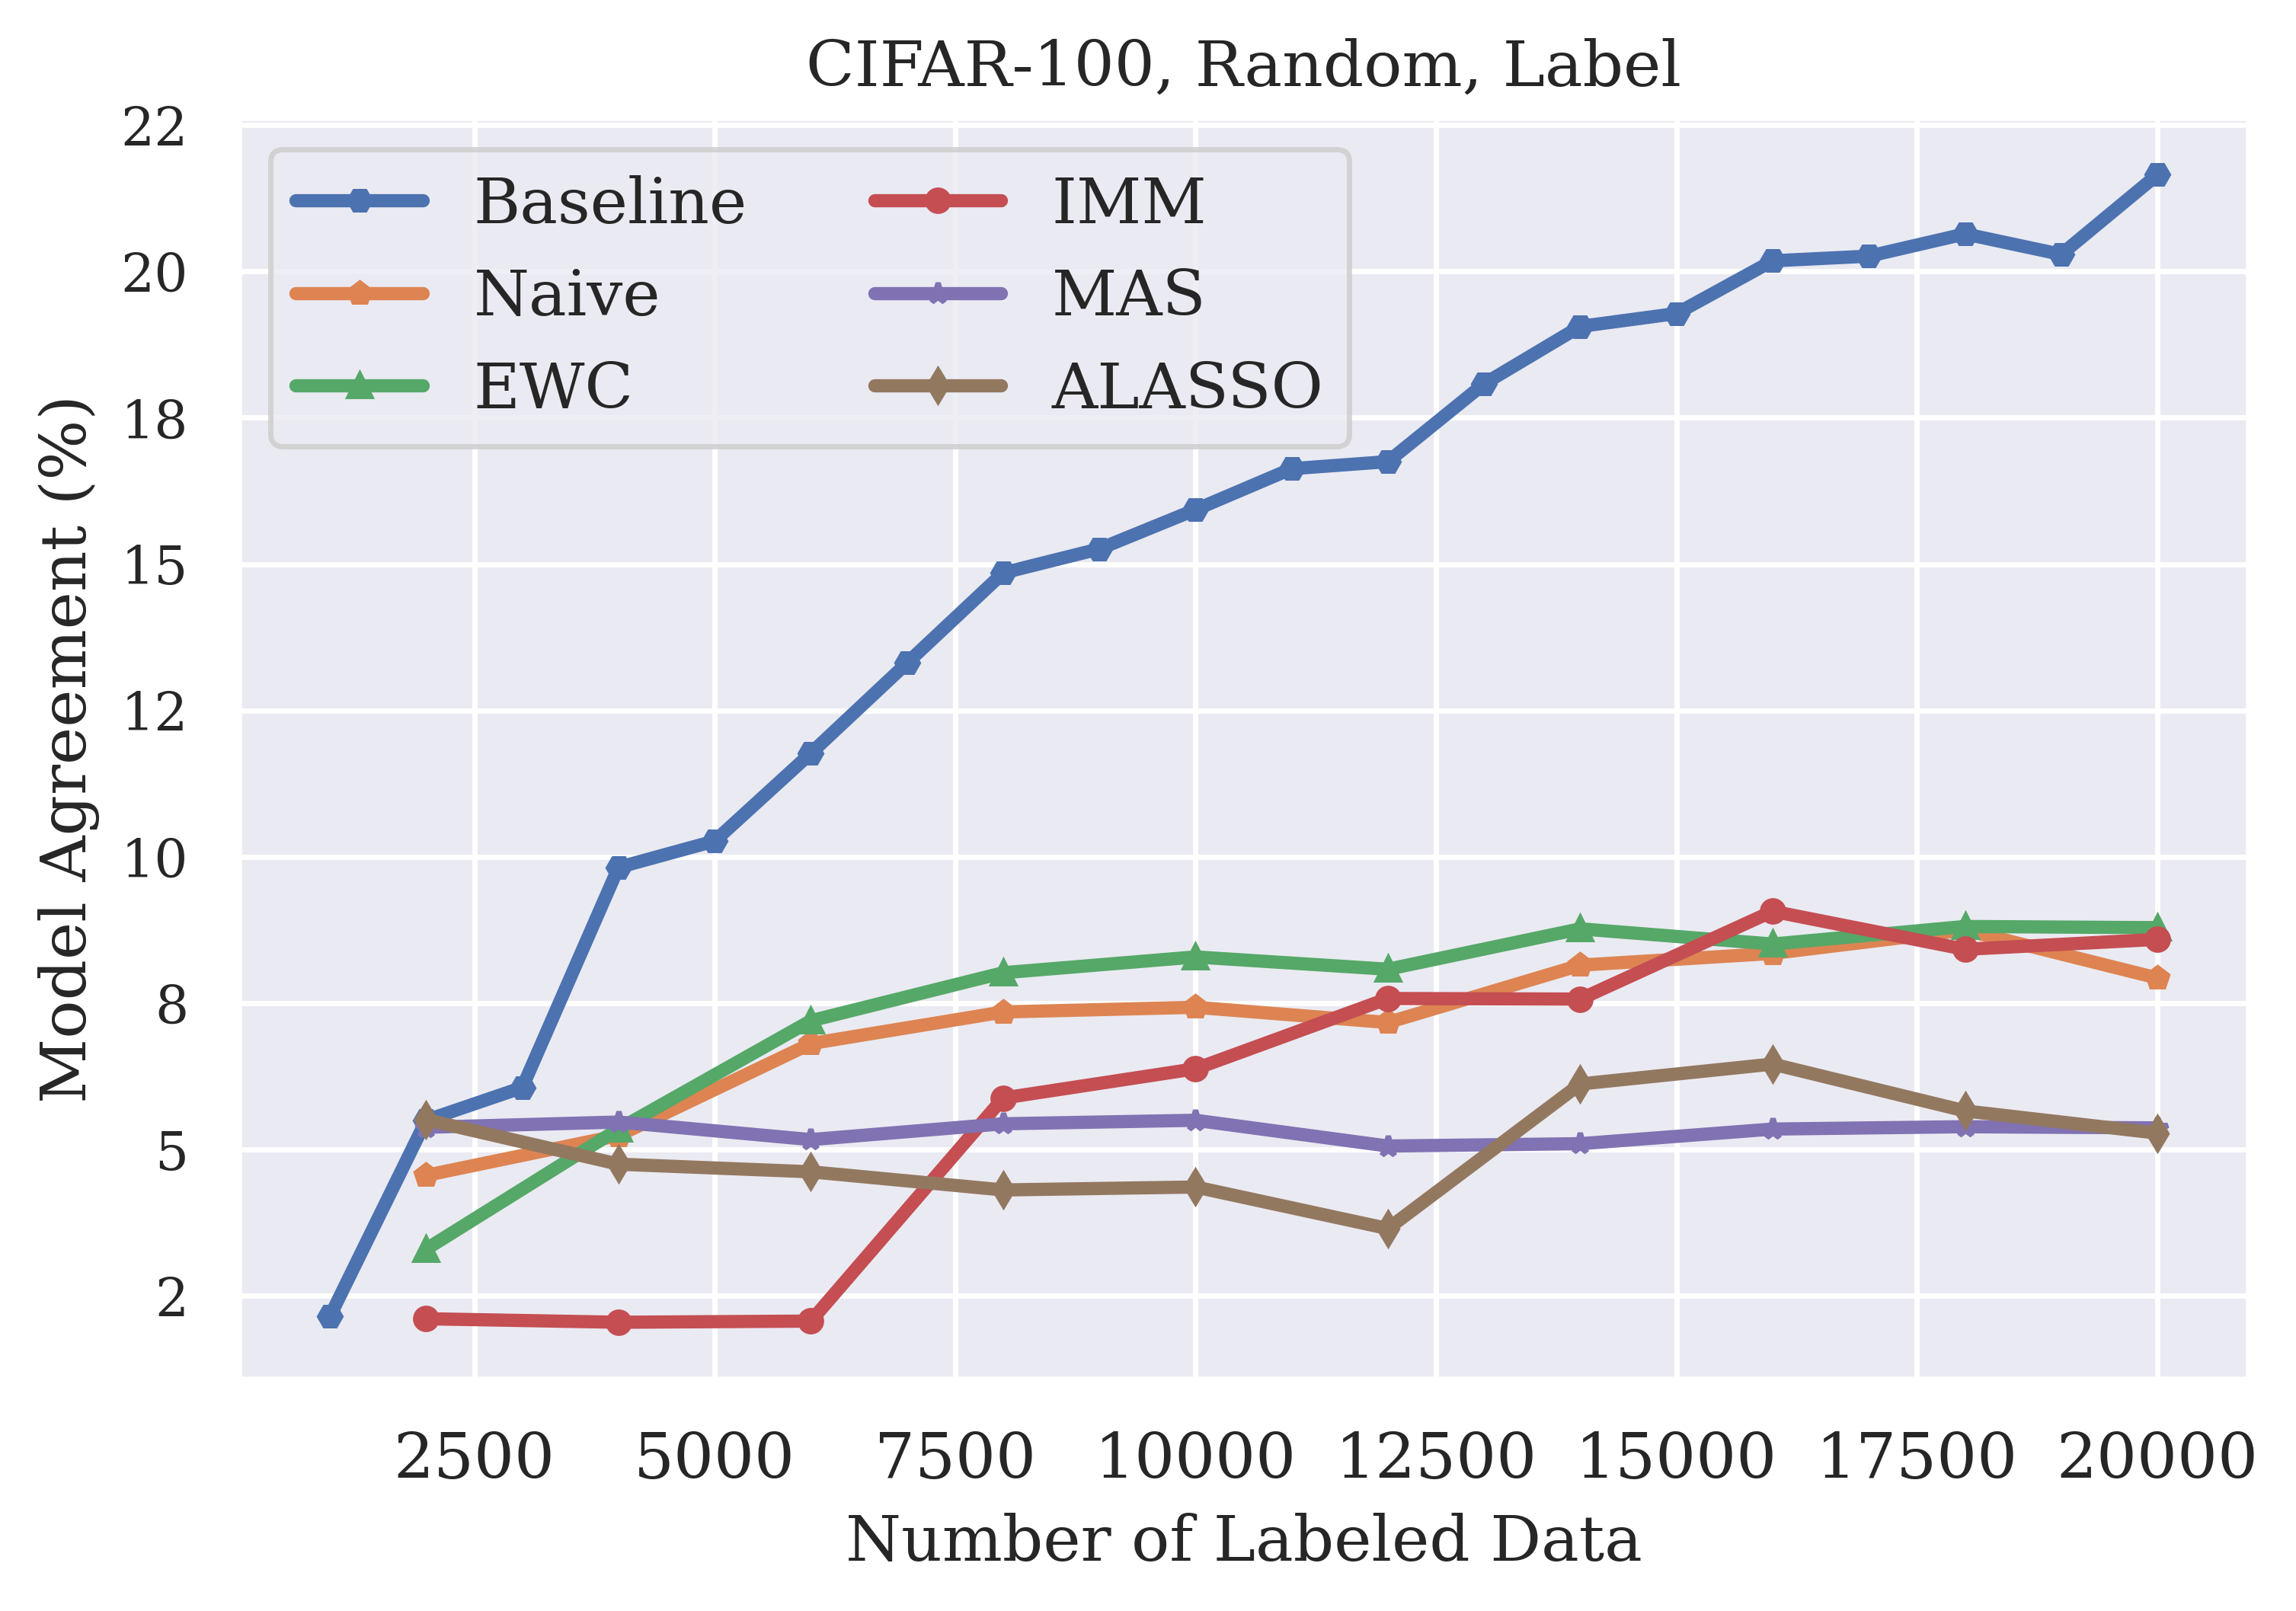
\includegraphics[width=0.48\linewidth]{images/results_CALMS/cifar100_label_random.png} \hfill
    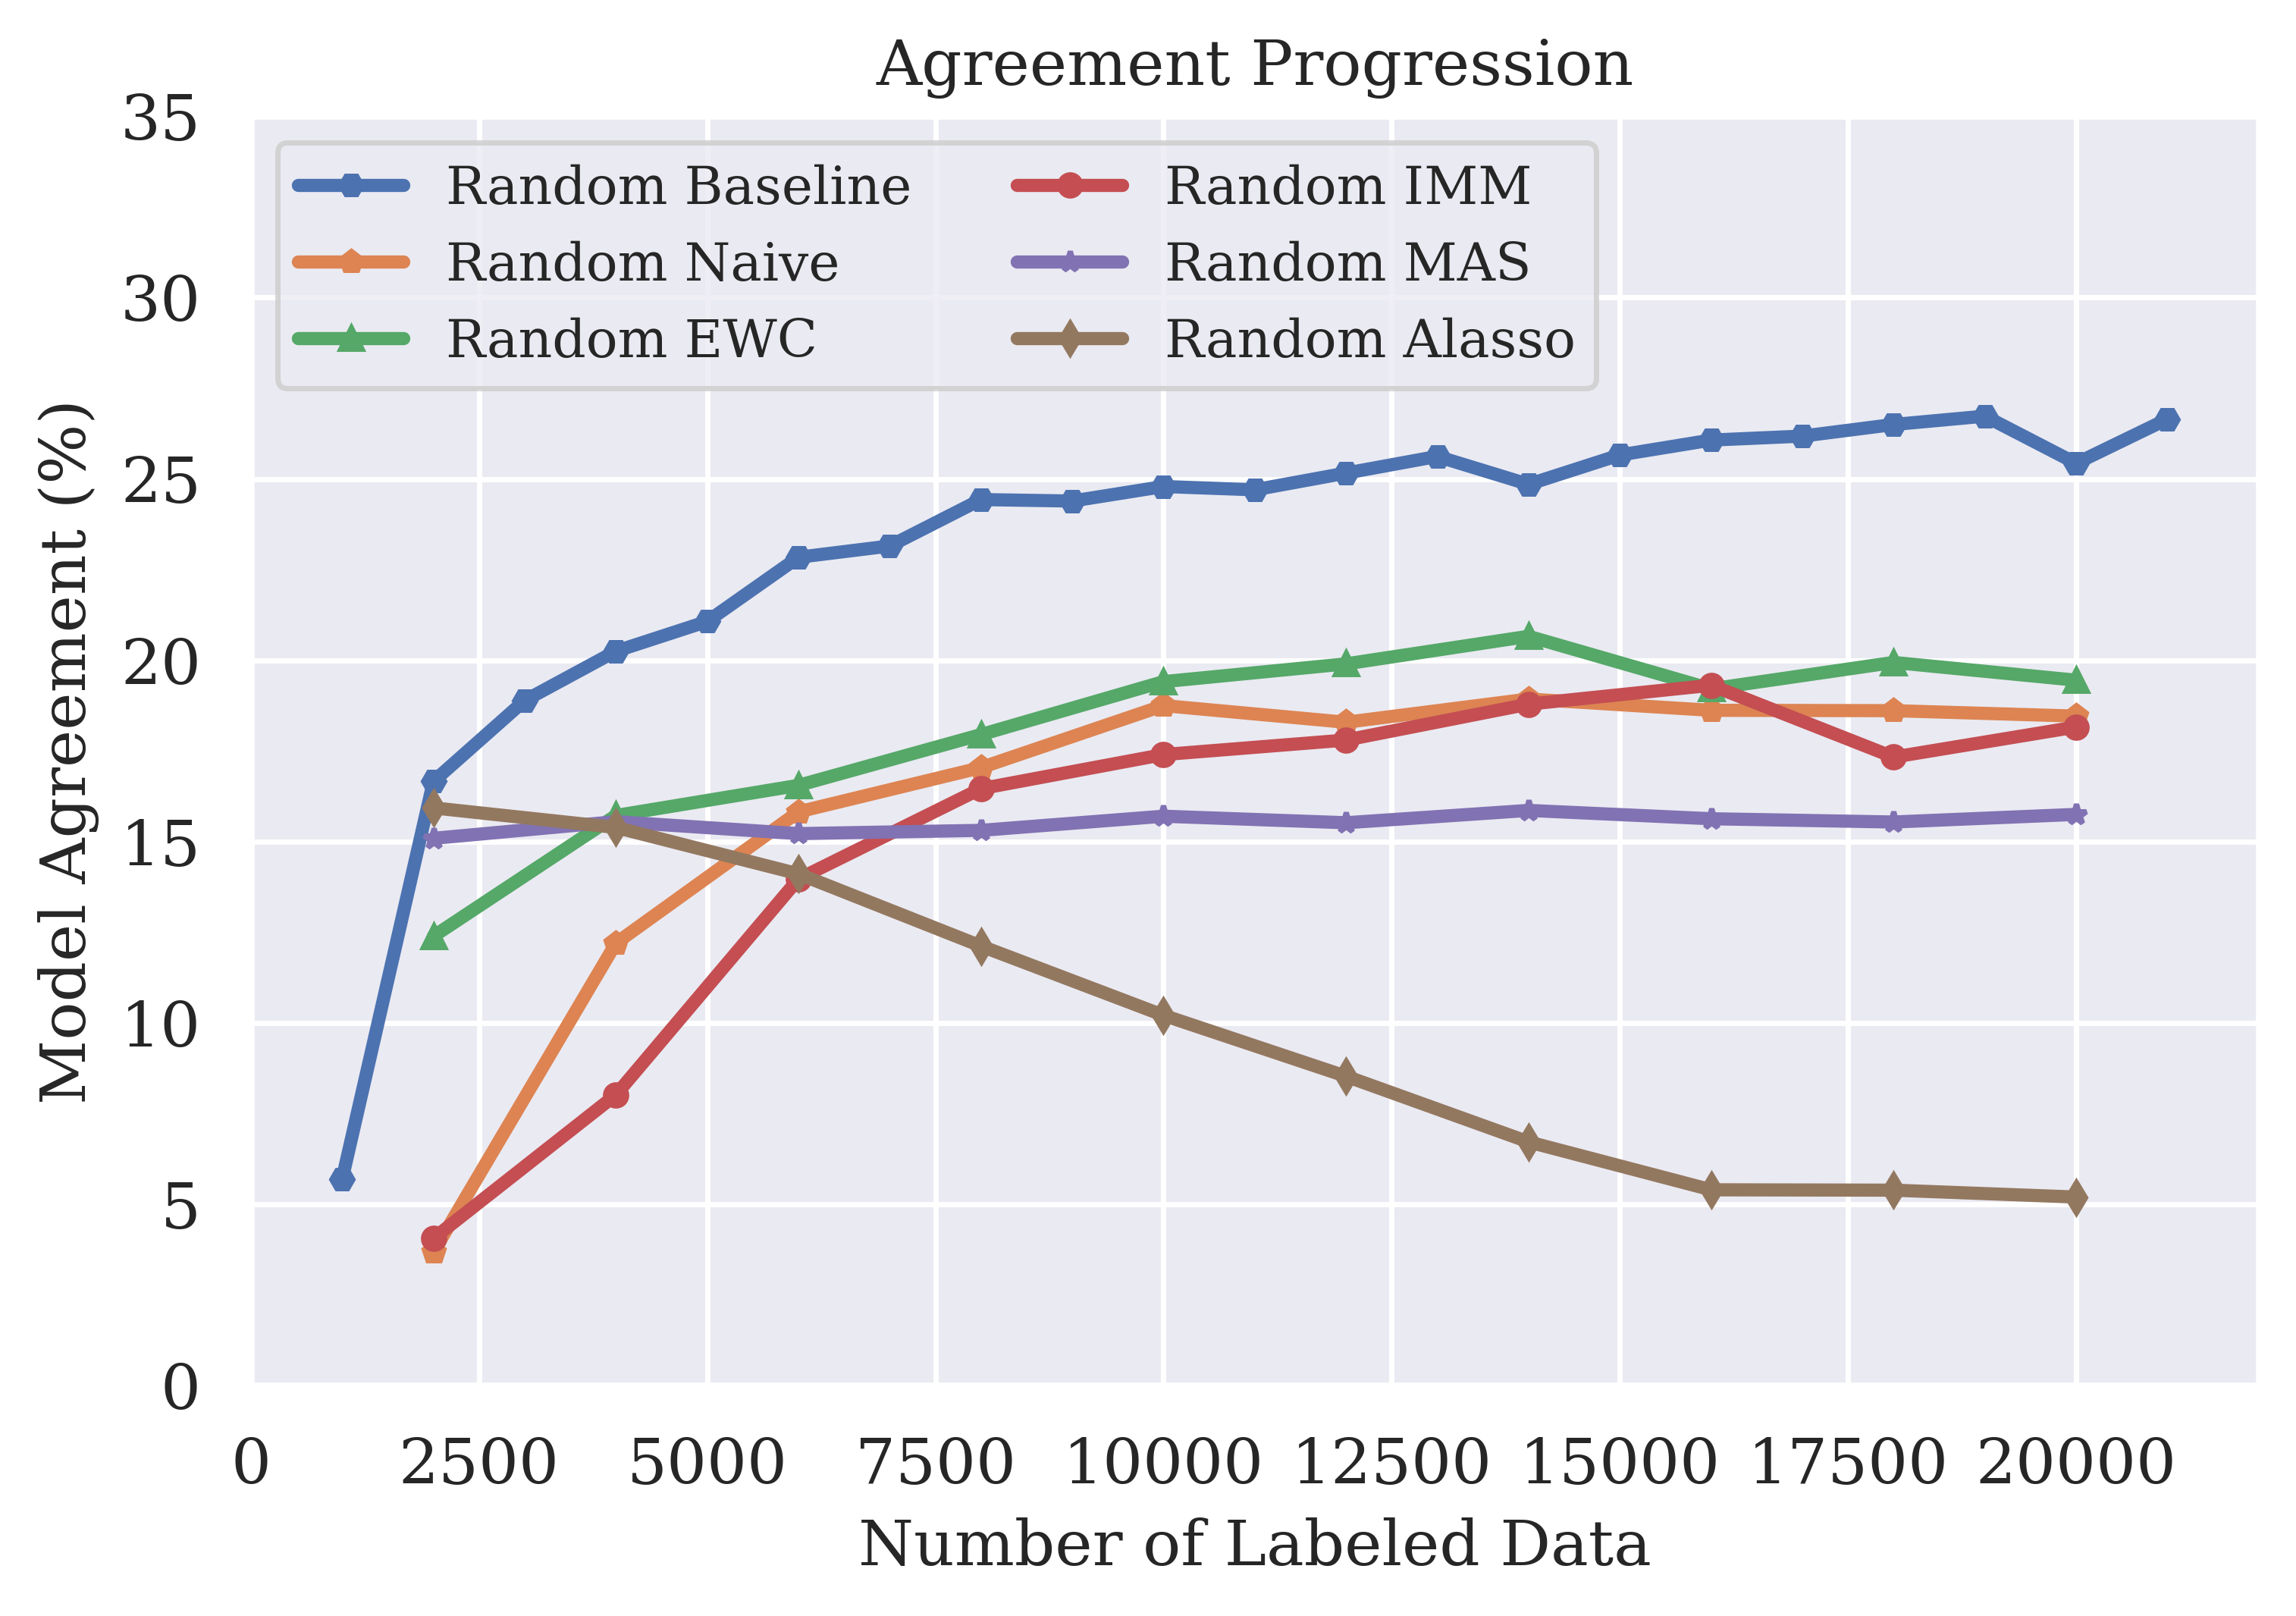
\includegraphics[width=0.48\linewidth]{images/results_CALMS/cifar100_softmax_random.png}
    \caption{Agreement Comparison for Model Stealing on CIFAR-100 using the Active Learning strategy Random. Left: Training with predicted class label,
    Right: Training with softmax output}
    \label{fig:CALMSCIFAR100Random}
\end{figure}

\begin{figure}[!htb]
    \centering
    \includegraphics[width=0.48\linewidth]{images/results_CALMS/cifar100_label_lc.png} \hfill
    \includegraphics[width=0.48\linewidth]{images/results_CALMS/cifar100_softmax_lc.png}
    \caption{Agreement Comparison for Model Stealing on CIFAR-100 using the Active Learning strategy \gls{lc}. Left: Training with predicted class label,
    Right: Training with softmax output}
    \label{fig:CALMSCIFAR100LC}
\end{figure}

\begin{figure}[!htb]
    \centering
    \includegraphics[width=0.48\linewidth]{images/results_CALMS/cifar100_label_bald.png} \hfill
    \includegraphics[width=0.48\linewidth]{images/results_CALMS/cifar100_softmax_bald.png}
    \caption{Agreement Comparison for Model Stealing on CIFAR-100 using the Active Learning strategy \gls{bald}. Left: Training with predicted class label,
    Right: Training with softmax output}
    \label{fig:CALMSCIFAR100BALD}
\end{figure}

\begin{figure}[!htb]
    \centering
    \includegraphics[width=0.48\linewidth]{images/results_CALMS/cifar100_label_coreset.png} \hfill
    \includegraphics[width=0.48\linewidth]{images/results_CALMS/cifar100_softmax_coreset.png}
    \caption{Agreement Comparison for Model Stealing on CIFAR-100 using the active learning strategy CoreSet. Left: Training with predicted class lLabel,
    Right: Training with softmax output}
    \label{fig:CALMSCIFAR100CoreSet}
\end{figure}

\subsubsection{VAAL and A-GEM}
\label{sec:Appendix:CALMS:VAALAGEM}
In the following we list the full results for the experiments using \gls{vaal} and \gls{a-gem} on the dataset MNIST, CIFAR-10 and CIFAR-100.
\begin{figure}[!htb]
    \centering
    \includegraphics[width=0.3\linewidth]{images/results_CALMS/mnist_vaal_agem.png} \hfill
    \includegraphics[width=0.3\linewidth]{images/results_CALMS/cifar_vaal_agem.png} \hfill
    \includegraphics[width=0.3\linewidth]{images/results_CALMS/cifar100_vaal_agem.png}
    \caption{Agreement Comparison for Model Stealing using \gls{vaal} and \gls{a-gem}. Left: MNIST, Middle: CIFAR-10, Right: CIFAR-100}
    \label{fig:CALMS_VAAL_AGEM}
\end{figure}

% Todo: Das hier sinnvoll strukturieren


\subsection{Effect of Data Augmentation on Model Stealing Attacks}
\label{sec:Appendix:EffectDataAugmentation}

While we managed to reproduce the findings of Pal et al. for CIFAR-10, we failed to do so for MNIST. Since multiple training hyperparameters of the experiments
presented in ActiveThief were not disclosed by the authors, we experiment with different combinations of hyperparameters, including varying the optimizer,
the learning rate, the number of training epochs, the batch size and switching between cold start and warm start for active learning. Sadly, we were still
not able to reproduce the results of ActiveThief on MNIST. After conducting the experiments in section \ref{sec:Evaluation:MS}, we decided to investigate
another hyperparameter: training with or without data augmentation. For this set of experiments, we leave all hyperparameters equal to the previous experiments,
apart from the data augmentation. We underline that using or not using data augmentation for model stealing refers to the thief dataset, not on the target
model dataset. Training the target model is always done using data augmentation. We perform the same model stealing attacks as before, using MNIST and
CIFAR-10 as target model dataset and present the results in figure \ref{fig:Evaluation:Results:CAL:EffectAugmentation}. When performing model stealing attacks
without data augmentation on CIFAR-10, we notice that model agreement, both for active learning and continual active learning, is significantly lower than
when using data augmentation. In this scenario, continual active learning with data augmentation performs on par with active learning without data augmentation.
However, when using MNISTas target model dataset, the results are reversed. Here, model agreement is significantly lower when using data augmentation.
More importantly, continual active learning without data augmentation shows performance comparable to active learning with data augmentation. \par

\begin{figure}[h]
    \centering
    \includegraphics[width=\linewidth]{images/results_CALMS/effect_data_augmentation.png}
    \caption[Effect of Data Augmentation on the success of Model Stealing Attacks]{Comparison of Model Agreement when using different data augmentation
    techniques. Left: Experiments with CIFAR-10. Right: Experiments with MNIST.}
    \label{fig:Evaluation:Results:CAL:EffectAugmentation}
\end{figure}

